\chapter{Worked Problems}\label{app:problems}

This appendix works through eight problems with complete solutions. They apply the tools of the book to concrete
markets: the Cournot and conduct models of \cref{ch:theory,ch:conduct}, the pricing theory of \cref{ch:diffprod},
and the demand models of \cref{ch:discrete,ch:logit,ch:blp}. Following a derivation and carrying one out are
different skills. A model becomes a working tool only once we have computed its equilibrium, estimated it on data
and checked the answer. Most of the problems use simulated data. We then know the truth, so we can see exactly what
each estimator recovers and where it fails.

The problems fall into four groups. \Cref{sec:C-cournot,sec:C-passthrough} treat a homogeneous good. The first works
out what Cournot competition, collusion and free entry imply for the relation between concentration and margins,
and what that relation can say about mergers. The second asks what the pass-through of a tax reveals about conduct,
and it re-estimates the cigarette tax regressions of \citet{Sumner1981}. \Cref{sec:C-logit-bertrand,sec:C-simulate}
compute price equilibria with differentiated products. The first does so for logit demand, proves that the
equilibrium is unique, and evaluates a merger and a tax. The second simulates 100 markets from a random coefficients
logit with multi-product pricing. \Cref{sec:C-vertical,sec:C-logit-est,sec:C-rc-est} estimate the vertical model,
the logit and the random coefficients logit on these simulated data. They compare the elasticities, markups,
recovered costs and merger predictions of the three models with the truth. \Cref{sec:C-autos} closes with real data,
the product file of the replication package of \citet{GriecoMurryYurukoglu2024}. It asks what simple demand models
say about the decline of markups in the U.S. automobile market, and it compares their answer with the full model of
that paper. \Cref{tab:C-map} lists the problems with the tools
and chapters each one draws on.

\begin{table}[tb]
\centering
\caption{The eight worked problems}
\label{tab:C-map}
\footnotesize
\begin{tabularx}{\textwidth}{@{}l>{\raggedright\arraybackslash}X>{\raggedright\arraybackslash}Xl@{}}
\toprule
Problem & Topic & Main tools & Builds on \\
\midrule
\ref{sec:C-cournot} & Cournot competition, collusion and entry, concentration and margins, mergers &
  Nash and subgame-perfect equilibrium, repeated games, OLS limits, Monte Carlo & Chapters \ref{ch:intro},
  \ref{ch:theory}, \ref{ch:mergers} \\
\addlinespace
\ref{sec:C-passthrough} & Tax pass-through and conduct in cigarettes & Comparative statics, two-way fixed effects,
  clustered inference, power, ad valorem taxes & Chapters \ref{ch:theory}, \ref{ch:conduct} \\
\addlinespace
\ref{sec:C-logit-bertrand} & Logit Bertrand pricing with single- and multi-product firms, a merger and a tax &
  Lambert W function, aggregative uniqueness proof, contraction mapping, upward pricing pressure & Chapters
  \ref{ch:diffprod}, \ref{ch:logit}, \ref{ch:mergers} \\
\addlinespace
\ref{sec:C-simulate} & Simulating a random coefficients logit market & Simulated shares, Morrow-Skerlos fixed
  point, sampling and simulation error & Chapter \ref{ch:blp} \\
\addlinespace
\ref{sec:C-vertical} & Estimating the vertical model & Share inversion, normalization, clustered OLS, implied
  costs & Chapter \ref{ch:discrete} \\
\addlinespace
\ref{sec:C-logit-est} & Estimating logit demand and recovering costs & Berry inversion, 2SLS, instrument
  strength, market bootstrap, joint GMM, omitted-heterogeneity bias & Chapters \ref{ch:logit}, \ref{ch:blp} \\
\addlinespace
\ref{sec:C-rc-est} & Random coefficients estimation, a comparison of three models and a merger & BLP contraction,
  2SLS, elasticity matrices, diversion, merger simulation & Chapters \ref{ch:blp}, \ref{ch:mergers} \\
\addlinespace
\ref{sec:C-autos} & Markups over time in U.S. automobiles & Nested logit, weak instruments with two endogenous
  regressors, second-choice data, decompositions & Chapters \ref{ch:intro}, \ref{ch:logit} \\
\bottomrule
\end{tabularx}

\vspace{3pt}
\begin{minipage}{0.97\textwidth}
\footnotesize Notes: Problems \ref{sec:C-simulate} to \ref{sec:C-rc-est} share one simulated data set and are best
read in order. The other problems can be read on their own.
\end{minipage}
\end{table}

Every problem has the same format. A short paragraph motivates it. A statement gives the data and the parameters
and poses parts (a), (b) and so on. The solution answers every part in order, with propositions and proofs for the
results it relies on. Theory proved in a chapter is restated in one line with a cross-reference and then used.
Computational notes describe the algorithms as numbered steps. Readers gain most by attempting each part before
reading its solution. The numerical parts need a scientific programming language with linear algebra, a root
finder and a random number generator. Every number computed in the solutions was produced by a Python script in
\texttt{figures/appC/src}, and numbers quoted from papers are cited to their tables or pages. The scripts read the
supplied data files in \texttt{figures/appC/data}, or the replication package used in \cref{sec:C-autos}. They draw
all simulated consumers, bootstrap samples and Monte Carlo samples with fixed seeds. Readers who draw their own random
numbers will obtain slightly different values.

Three conventions need care across the problems. First, $\delta$ is the discount factor in \cref{sec:C-cournot}
and mean utility in the other problems. Second, in \cref{sec:C-cournot,sec:C-passthrough} the symbol $\varepsilon$
is the market elasticity written as a positive number, as in the notation list. From \cref{sec:C-logit-bertrand}
on, we report elasticity matrices with entries $\varepsilon_{jk} = \frac{\partial s_j}{\partial p_k}\frac{p_k}{s_j}$.
Own elasticities are then negative, and the positive own elasticity of the notation list is $-\varepsilon_{jj}$.
Third, $\Phi$ always denotes the logit denominator, while $\Lambda_t$ and $\Gamma_t$ are the matrices of the
Morrow-Skerlos fixed point of \cref{sec:C-simulate}. Symbols used in a single problem are defined where they first
appear.

\section{Cournot competition, entry, collusion and the concentration-margin relation}\label{sec:C-cournot}

Cross-industry studies in the structure-conduct-performance tradition relate profitability to
concentration. \citet{Bain1951} compared profit rates across industries, and later work regressed price-cost
margins on concentration \citep{Schmalensee1989}. This problem works out what four canonical models of a homogeneous-good
industry imply for that relation, and what the relation can and cannot say about mergers. The four models
are Cournot competition and perfect collusion, each with a fixed number of firms and with free entry. Two
extensions add firms with different costs and mergers. A computational part simulates a cross-section of
industries and compares the merger predictions of the regression with the true equilibrium effects. The
theory behind the problem is developed in \cref{sec:02-cournot,sec:02-entry,sec:02-collusion}, and the
cross-industry regression is studied in \cref{sec:01-montecarlo}.

\subsection{Statement}\label{sec:C-cournot-statement}

A homogeneous good has linear inverse demand $P(Q) = a - bQ$, where $Q$ is total output, $a > c > 0$ and
$b > 0$. Every active firm pays a fixed cost $F > 0$ per period and produces at constant marginal cost $c$. The
Lerner index is $L = \frac{P - c}{P}$, the Herfindahl index is $\HHI = \sum_i s_i^2$ with market shares
$s_i = \frac{q_i}{Q}$, and $\varepsilon = -\frac{\dd Q}{\dd P}\frac{P}{Q}$ is the market elasticity of demand,
written as a positive number. Two constants recur. The \emph{market-size index} is
$x \equiv \frac{a - c}{\sqrt{bF}}$, and the \emph{profit scale} is $k \equiv \frac{(a - c)^2}{b}$.

\begin{enumerate}[label=(\alph*)]
\item There are $N$ firms that choose outputs simultaneously. Describe the game and the equilibrium concept.
  Show that the equilibrium is unique and symmetric. Compute the price, outputs, profits, $L$ and $\HHI$, and
  verify that $L = \frac{\HHI}{\varepsilon}$.
\item Firms first decide whether to enter and then play the game of part (a). Treating the number of firms as
  continuous, find the free-entry number of firms and the resulting price, outputs, $L$ and $\HHI$.
\item Repeat parts (a) and (b) when the active firms collude perfectly, charging the monopoly price and
  splitting output equally. Show that collusion is not a Nash equilibrium of the one-shot game. Find the
  discount factor above which grim-trigger strategies sustain collusion in the infinitely repeated game.
\item Describe the relation between $\HHI$ and $L$ in the four cases.
\item An economist posits $\E[L] = \beta_0 + \beta_1\HHI$ and estimates it on a cross-section of industries.
  Does the specification make sense under each model? Are the estimates consistent, and for what? Are they
  useful for predicting the effect of a merger?
\item Let firm $i$ have its own constant marginal cost $c_i$, with every firm active. Show that
  $L_i = \frac{s_i}{\varepsilon}$ and $\sum_i s_iL_i = \frac{\HHI}{\varepsilon}$. Show that a mean-preserving spread
  of costs that keeps every firm active raises $\HHI$ and the share-weighted Lerner index, leaves the price
  unchanged and raises welfare.
\item Evaluate every object of parts (a) to (c) for $a = 10$, $c = 2$, $b = 1$ and $F = 1$, including consumer
  surplus, total welfare and the welfare-maximizing number of firms.
\item In the symmetric Cournot model, study the profitability of a merger of two firms and of $k_M$ firms.
  Compare the change in $\HHI$ computed from pre-merger shares with the equilibrium change. Find the marginal
  cost of the merged firm below which the merger does not raise the price.
\item (Computational.) Simulate a cross-section of Cournot industries, estimate the regression of part (e),
  and compare the merger effects it predicts with the true equilibrium effects.
\end{enumerate}

\subsection{Solution}\label{sec:C-cournot-solution}

\casehead{Part (a)}
The game has players $i = 1, \dots, N$. Each player chooses an output $q_i \ge 0$, all players move
simultaneously, and all primitives are common knowledge. Firm $i$'s payoff is
\begin{equation}\label{eq:C-cournot-profit}
\pi_i(q_i, q_{-i}) = \big(a - bQ - c\big)q_i - F, \qquad Q = q_i + Q_{-i}, \quad Q_{-i} = \sum_{j \ne i} q_j .
\end{equation}
A \emph{Nash equilibrium} is a profile $q^* = (q_1^*, \dots, q_N^*)$ such that $q_i^*$ maximizes
$\pi_i(q_i, q_{-i}^*)$ for every $i$. The fixed cost lowers the profit of an active firm but does not affect
its output choice.

Profit is strictly concave in the firm's own output, since
\begin{equation*}
\frac{\partial \pi_i}{\partial q_i} = a - c - bQ_{-i} - 2bq_i, \qquad
\frac{\partial^2 \pi_i}{\partial q_i^2} = -2b < 0 .
\end{equation*}
The unique best response to rivals' total output $Q_{-i}$ is therefore
\begin{equation}\label{eq:C-cournot-br}
BR_i(Q_{-i}) = \max\Big\{0, \frac{a - c - bQ_{-i}}{2b}\Big\}.
\end{equation}

\begin{proposition}[Linear Cournot equilibrium]\label{prop:C-cournot}
With $a > c$, the Cournot game has a unique Nash equilibrium. It is symmetric, every firm is active, and
\begin{equation}\label{eq:C-cournot-q}
q = \frac{a - c}{b(N + 1)}, \qquad Q = \frac{N(a - c)}{b(N + 1)}, \qquad P = \frac{a + Nc}{N + 1}.
\end{equation}
\end{proposition}

\begin{proof}
We proceed in three steps. First, total output is positive in any equilibrium. If $Q = 0$, every firm faces
$Q_{-i} = 0$, and \eqref{eq:C-cournot-br} gives $BR_i(0) = \frac{a - c}{2b} > 0$, a contradiction. Second,
every firm is active. An active firm $l$ satisfies the first-order condition $a - c - bQ - bq_l = 0$, so
\begin{equation*}
bq_l = a - c - bQ .
\end{equation*}
Since $q_l > 0$, this gives $a - c - bQ > 0$. A firm $i$ with $q_i = 0$ would need
$\frac{\partial \pi_i}{\partial q_i}\big|_{q_i = 0} = a - c - bQ \le 0$, which contradicts the previous
inequality. Third, every firm satisfies $bq_i = a - c - bQ$, so all outputs are equal. Summing over the $N$
firms gives
\begin{align*}
bQ &= N(a - c) - NbQ, \\
Q &= \frac{N(a - c)}{b(N + 1)} .
\end{align*}
Total output is unique, so each output $q = \frac{Q}{N}$ is unique. The price is
$P = a - bQ = \frac{a(N + 1) - N(a - c)}{N + 1} = \frac{a + Nc}{N + 1}$.
\end{proof}

The remaining objects follow by substitution. The margin and the profit are
\begin{align}
P - c &= \frac{a + Nc - (N + 1)c}{N + 1} = \frac{a - c}{N + 1} = bq, \label{eq:C-cournot-margin}\\
\pi &= (P - c)q - F = \frac{a - c}{N + 1}\cdot\frac{a - c}{b(N + 1)} - F = \frac{k}{(N + 1)^2} - F .
\label{eq:C-cournot-pi}
\end{align}
The Lerner index divides the margin by the price, and every firm has share $\frac{1}{N}$:
\begin{equation}\label{eq:C-cournot-LH}
L = \frac{a - c}{N + 1}\cdot\frac{N + 1}{a + Nc} = \frac{a - c}{a + Nc}, \qquad
\HHI = N\cdot\frac{1}{N^2} = \frac{1}{N}.
\end{equation}
With linear demand $-\frac{\dd Q}{\dd P} = \frac{1}{b}$, so the elasticity at the equilibrium is
\begin{equation*}
\varepsilon = \frac{P}{bQ} = \frac{a + Nc}{N + 1}\cdot\frac{N + 1}{N(a - c)} = \frac{a + Nc}{N(a - c)} .
\end{equation*}
The check is direct:
$\frac{\HHI}{\varepsilon} = \frac{1}{N}\cdot\frac{N(a - c)}{a + Nc} = \frac{a - c}{a + Nc} = L$. The relation
holds for any demand curve. Firm $i$'s first-order condition $P + q_iP'(Q) = c$ gives
$\frac{P - c}{P} = -\frac{q_iP'}{P} = \frac{q_i}{Q}\cdot\frac{1}{\varepsilon}$, and symmetry sets
$\frac{q_i}{Q} = \frac{1}{N} = \HHI$ (\cref{sec:02-cournot-markups}).

\casehead{Part (b)}
Entry adds a first stage. In stage 1, a large pool of identical potential entrants decide simultaneously
whether to enter and pay $F$. In stage 2, the $N$ entrants observe $N$ and play the Cournot game of part (a).
The solution concept is \emph{subgame-perfect equilibrium}. \Cref{prop:C-cournot} fixes play in every
stage-2 subgame, so an entrant earns $\pi(N) = \frac{k}{(N + 1)^2} - F$, which is strictly decreasing in $N$.
In equilibrium no entrant regrets entering and no outsider wants to enter, so the number of firms $N^e$
satisfies $\pi(N^e) \ge 0 \ge \pi(N^e + 1)$. Treating $N$ as continuous gives the zero-profit condition
$\pi(N^e) = 0$:
\begin{align}
(N^e + 1)^2 &= \frac{(a - c)^2}{bF} = x^2, \notag\\
N^e &= x - 1 = \frac{a - c}{\sqrt{bF}} - 1 . \label{eq:C-Ne}
\end{align}
The free-entry outcomes follow from \eqref{eq:C-cournot-q} and \eqref{eq:C-cournot-margin} with
$\frac{a - c}{N^e + 1} = \sqrt{bF}$:
\begin{align}
P^e &= c + \frac{a - c}{N^e + 1} = c + \sqrt{bF}, \qquad
q^e = \frac{a - c}{b(N^e + 1)} = \frac{\sqrt{bF}}{b} = \sqrt{\frac{F}{b}}, \notag\\
Q^e &= \frac{a - P^e}{b} = \frac{a - c - \sqrt{bF}}{b}, \notag\\
L^e &= \frac{P^e - c}{P^e} = \frac{\sqrt{bF}}{c + \sqrt{bF}}, \qquad
\HHI^e = \frac{1}{N^e} = \frac{1}{x - 1} = \frac{\sqrt{bF}}{a - c - \sqrt{bF}} . \label{eq:C-free-entry}
\end{align}
Each entrant earns $(P^e - c)q^e - F = \sqrt{bF}\sqrt{\frac{F}{b}} - F = 0$. The formulas require $N^e \ge 1$,
that is, $x \ge 2$, or equivalently $0 < F \le \frac{(a - c)^2}{4b}$. The Cournot rule survives entry. The elasticity at
$P^e$ is $\varepsilon^e = \frac{P^e}{bQ^e} = \frac{c + \sqrt{bF}}{a - c - \sqrt{bF}}$, and
$\frac{\HHI^e}{\varepsilon^e} = L^e$. Under free entry the dollar margin $\sqrt{bF}$ is fixed by technology
and the slope of demand. A larger intercept $a$ brings more firms and leaves the margin unchanged. With the
integer constraint, $N^e$ is the integer part of $x - 1$ (\cref{sec:02-mw-integer}).

\casehead{Part (c)}
Under perfect collusion with $N$ firms fixed, the firms choose total output to maximize joint profit
\begin{equation*}
\Pi(Q) = (a - bQ - c)Q - NF, \qquad \Pi''(Q) = -2b < 0 .
\end{equation*}
The first-order condition $a - c - 2bQ = 0$ gives the monopoly outcome
\begin{equation}\label{eq:C-monopoly}
Q^m = \frac{a - c}{2b}, \qquad P^m = a - bQ^m = \frac{a + c}{2}, \qquad P^m - c = \frac{a - c}{2}.
\end{equation}
Each firm produces $q = \frac{Q^m}{N} = \frac{a - c}{2bN}$ and earns $\pi = \frac{a - c}{2}\cdot\frac{a - c}{2bN} - F
= \frac{k}{4N} - F$. The Lerner index is $L = \frac{a - c}{a + c}$ for every $N$, and $\HHI = \frac{1}{N}$. The
elasticity at the monopoly price is $\varepsilon(P^m) = \frac{P^m}{bQ^m} = \frac{a + c}{a - c}$, so
$L = \frac{1}{\varepsilon(P^m)}$, the monopoly inverse-elasticity rule. Price, total output and the margin do not
depend on $N$. Profit per firm and $\HHI$ fall as $N$ rises.

Collusion is not a Nash equilibrium of the one-shot game when $N \ge 2$. Suppose every rival produces
$\frac{Q^m}{N}$. At $q_i = \frac{Q^m}{N}$ the marginal profit of firm $i$ is
\begin{equation*}
\frac{\partial \pi_i}{\partial q_i} = a - c - bQ^m - b\frac{Q^m}{N} = \frac{a - c}{2} - \frac{a - c}{2N}
= \frac{(N - 1)(a - c)}{2N} > 0 .
\end{equation*}
Each firm gains by expanding, because it bears only its own share of the price reduction that its extra
output causes.

Collusion can be sustained in the infinitely repeated game. In periods $t = 0, 1, 2, \dots$ the $N$ firms play
the stage game of part (a). Outputs are observed at the end of each period. In this problem $\delta \in (0, 1)$
denotes the discount factor, as in \cref{ch:collusion-theory} (in the demand chapters $\delta$ is mean utility).
Firm $i$ maximizes $\sum_{t \ge 0}\delta^t\pi_{it}$. Under \emph{grim-trigger} strategies \citep{Friedman1971}, each
firm produces $\frac{Q^m}{N}$ in period 0 and in every period that follows no deviation. After any deviation every
firm produces the Cournot output $\frac{a - c}{b(N + 1)}$ forever.

\begin{proposition}[Threshold discount factor for Cournot collusion]\label{prop:C-delta}
Grim-trigger strategies form a subgame-perfect equilibrium that sustains the monopoly outcome if and only if
\begin{equation}\label{eq:C-delta}
\delta \ge \delta^*(N) \equiv \frac{(N + 1)^2}{N^2 + 6N + 1}.
\end{equation}
The threshold satisfies $\delta^*(2) = \frac{9}{17}$, is strictly increasing in $N$ for $N > 1$, and
tends to one as $N \to \infty$.
\end{proposition}

\begin{proof}
The fixed cost enters every period's payoff equally, so it cancels from every incentive constraint. What remains is
\cref{prop:12-cournot}, which gives the threshold, its monotonicity and its limit. At $N = 2$ the threshold is
$\frac{9}{4 + 12 + 1} = \frac{9}{17}$.
\end{proof}

\Cref{fig:C-delta} plots the threshold together with the Bertrand benchmark. In the Bertrand supergame a
deviator undercuts slightly and takes the whole monopoly profit $\pi^m$, after which profits are zero. The
condition $\frac{\pi^m}{N(1 - \delta)} \ge \pi^m$ gives $\delta \ge 1 - \frac{1}{N}$ (\cref{prop:12-bertrand}).
\citet[Section~6.3.2.1]{Tirole1988} uses this threshold to formalize the old claim that concentration facilitates
tacit collusion.
The two thresholds cross between $N = 2$ and $N = 3$. Cournot collusion is harder to sustain for $N = 2$
($\frac{9}{17} = 0.529$ against $0.5$) and easier for every $N \ge 3$ ($\frac{4}{7} = 0.571$ against $0.667$ at
$N = 3$). For large $N$, $1 - \delta^*(N) = \frac{4N}{N^2 + 6N + 1}$ is close to $\frac{4}{N}$, four
times the Bertrand slack $\frac{1}{N}$. Cournot reversion is a mild punishment, but the one-shot gain from
deviating is also small, because the deviator expands only to its best response.

\begin{figure}[htbp]
\centering
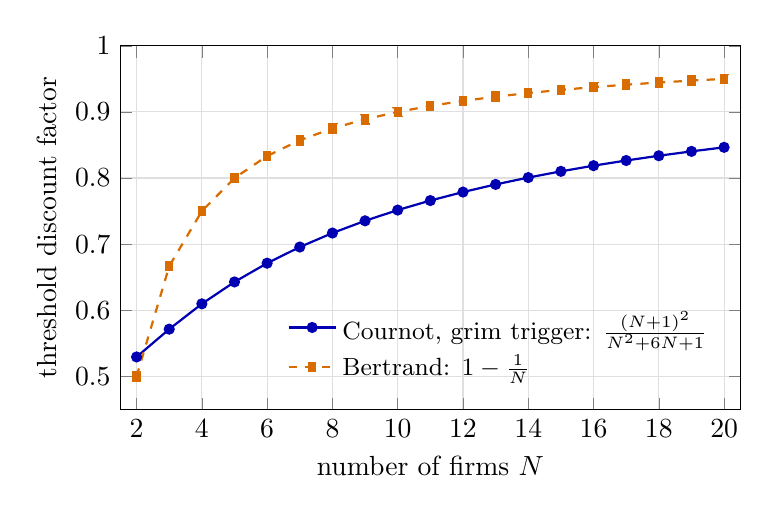
\begin{tikzpicture}
\begin{axis}[
  width=0.78\textwidth, height=6.2cm,
  xlabel={number of firms $N$}, ylabel={threshold discount factor},
  xmin=1.5, xmax=20.5, ymin=0.45, ymax=1.0,
  xtick={2,4,6,8,10,12,14,16,18,20},
  ytick={0.5,0.6,0.7,0.8,0.9,1.0},
  yticklabel style={/pgf/number format/fixed, /pgf/number format/precision=1},
  grid=major, grid style={gray!25},
  legend style={draw=none, fill=none, font=\small, at={(0.97,0.05)}, anchor=south east},
  legend cell align=left,
]
\addplot[blue!70!black, thick, mark=*, mark size=1.6pt, samples at={2,3,...,20}]
  {(x + 1)^2/(x^2 + 6*x + 1)};
\addlegendentry{Cournot, grim trigger: $\frac{(N + 1)^2}{N^2 + 6N + 1}$}
\addplot[orange!85!black, thick, dashed, mark=square*, mark size=1.5pt, samples at={2,3,...,20}]
  {1 - 1/x};
\addlegendentry{Bertrand: $1 - \frac{1}{N}$}
\end{axis}
\end{tikzpicture}
\caption{Lowest discount factor at which grim-trigger strategies sustain the monopoly outcome among $N$
symmetric firms, for Cournot and Bertrand stage games with linear demand and constant marginal cost. The
Cournot threshold does not depend on $a$, $b$, $c$ or $F$.}
\label{fig:C-delta}
\end{figure}

\begin{remark}
Grim trigger is not the harshest credible punishment. \citet{Abreu1986} studies stick-and-carrot
punishments, in which firms produce more than the Cournot output for one period and then return to
collusion. These punish deviators more severely and sustain the monopoly outcome at lower discount factors
than \eqref{eq:C-delta}. \Cref{ch:collusion-theory} develops optimal punishments.
\end{remark}

With free entry, collusive play in stage 2 yields per-firm profit $\pi(N) = \frac{k}{4N} - F$. The free-entry
condition $\pi(N^m) = 0$, with $N$ continuous, gives
\begin{equation}\label{eq:C-Nm}
N^m = \frac{(a - c)^2}{4bF} = \frac{x^2}{4}.
\end{equation}
Price and total output stay at the monopoly values, so entry only changes how $Q^m$ is divided:
\begin{equation*}
q^m = \frac{Q^m}{N^m} = \frac{a - c}{2b}\cdot\frac{4bF}{(a - c)^2} = \frac{2F}{a - c}, \qquad
L = \frac{a - c}{a + c}, \qquad \HHI^m = \frac{1}{N^m} = \frac{4bF}{(a - c)^2}.
\end{equation*}
Total fixed costs equal the monopoly profit, $N^mF = \frac{(a - c)^2}{4b} = (P^m - c)Q^m$, so entry dissipates
the whole rent. Consumers gain nothing, because the price stays at $P^m$. Collusion attracts more entrants
than Cournot competition:
\begin{equation}\label{eq:C-Nm-Ne}
N^m - N^e = \frac{x^2}{4} - x + 1 = \Big(\frac{x}{2} - 1\Big)^2 \ge 0,
\end{equation}
with equality only at $x = 2$, where both equal one. The higher collusive margin draws firms in until profit is
again zero. The collusive outcome with $N^m$ firms is an equilibrium of the repeated game only if $\delta \ge
\delta^*(N^m)$. Lower fixed costs raise $N^m$ and push the threshold toward one, so free entry also
makes collusion harder to enforce.

\casehead{Part (d)}
\Cref{tab:C-cournot-cases} collects the four regimes (the closed forms are also in
\cref{tab:02-linear-cournot}). Under Cournot conduct with $N$ fixed, substitute $N = \frac{1}{\HHI}$ in
the elasticity of part (a):
\begin{equation}\label{eq:C-LH-curve}
\varepsilon = \frac{a\HHI + c}{a - c}, \qquad L = \frac{\HHI}{\varepsilon} = \frac{(a - c)\HHI}{a\HHI + c}.
\end{equation}
The derivatives
\begin{align*}
\frac{\dd L}{\dd\HHI} &= \frac{(a - c)(a\HHI + c) - (a - c)\HHI a}{(a\HHI + c)^2} = \frac{c(a - c)}{(a\HHI + c)^2} > 0,\\
\frac{\dd^2 L}{\dd\HHI^2} &= -\frac{2ac(a - c)}{(a\HHI + c)^3} < 0
\end{align*}
show an increasing and concave curve. It runs from $L = 0$ at $\HHI = 0$ to the monopoly value
$\frac{a - c}{a + c}$ at $\HHI = 1$. When $N$ is set outside the model, the curve is the causal effect of
concentration on margins in an industry with given $(a, c)$.

\begin{table}[htbp]
\centering
\begin{threeparttable}
\caption{Concentration and margins in the linear homogeneous-good industry under four regimes}
\label{tab:C-cournot-cases}
\small
\setlength{\tabcolsep}{4pt}
\begin{tabular}{@{}lccccc>{\raggedright\arraybackslash}p{2.75cm}@{}}
\toprule
Regime & $N$ & $P$ & $q$ & $L$ & $\HHI$ & Relation of $L$ to $\HHI$ \\
\midrule
Cournot, fixed $N$ & $N$ & $\frac{a + Nc}{N + 1}$ & $\frac{a - c}{b(N + 1)}$ & $\frac{a - c}{a + Nc}$ &
  $\frac{1}{N}$ & increasing, concave, causal \\
\addlinespace
Cournot, free entry & $x - 1$ & $c + \sqrt{bF}$ & $\sqrt{\frac{F}{b}}$ & $\frac{\sqrt{bF}}{c + \sqrt{bF}}$ &
  $\frac{\sqrt{bF}}{a - c - \sqrt{bF}}$ & same curve, both endogenous \\
\addlinespace
Collusion, fixed $N$ & $N$ & $\frac{a + c}{2}$ & $\frac{a - c}{2bN}$ & $\frac{a - c}{a + c}$ & $\frac{1}{N}$ &
  flat \\
\addlinespace
Collusion, free entry & $\frac{x^2}{4}$ & $\frac{a + c}{2}$ & $\frac{2F}{a - c}$ & $\frac{a - c}{a + c}$ &
  $\frac{4bF}{(a - c)^2}$ & opposite directions when $a$ or $c$ vary \\
\bottomrule
\end{tabular}
\begin{tablenotes}\footnotesize
\item Notes: Inverse demand $P = a - bQ$, marginal cost $c$, fixed cost $F$, and $x = \frac{a - c}{\sqrt{bF}}$.
Free-entry columns treat $N$ as continuous and require $x \ge 2$. Under Cournot conduct $L = \frac{\HHI}{\varepsilon}$,
and under collusion $L = \frac{1}{\varepsilon}$, with $\varepsilon$ evaluated at the equilibrium price.
\end{tablenotes}
\end{threeparttable}
\end{table}

With free entry, Cournot industries stay on the curve \eqref{eq:C-LH-curve}, but $\HHI^e$ and $L^e$ are now
both outcomes of $(a, b, c, F)$. Write $r = \sqrt{bF}$, so that $\HHI^e = \frac{r}{a - c - r}$ and
$L^e = \frac{r}{c + r}$. Each primitive moves the pair differently. A higher $F$ or $b$ raises $r$ and with it
both $\HHI^e$ and $L^e$, so the industry moves up along the curve. A higher $a$ lowers $\HHI^e$ and leaves $L^e$
unchanged. A higher $c$ raises $\HHI^e$ and lowers $L^e$. Across industries, the sign of the association
between $\HHI$ and $L$ therefore depends on which primitive varies.

Under collusion with $N$ fixed, $L = \frac{a - c}{a + c}$ for every $N$, so the relation is flat. With free
entry, $L$ still depends only on $(a, c)$, while $\HHI^m = \frac{4bF}{(a - c)^2}$. Variation in $F$ or $b$
moves $\HHI^m$ alone. A higher $a$ raises $L$ and lowers $\HHI^m$, and a higher $c$ does the reverse, so
variation in $a$ or $c$ moves the two indices in opposite directions.

Differences in conduct weaken, and can reverse, the positive Cournot relation. Compare a Cournot industry and
a collusive industry with the same primitives. With $N$ fixed both have $\HHI = \frac{1}{N}$, and the collusive
industry has the higher margin, since $\frac{a - c}{a + c} > \frac{a - c}{a + Nc}$ for $N > 1$. With free entry,
collusion again raises the margin, because $P^e = c + \sqrt{bF} \le \frac{a + c}{2} = P^m$ whenever $x \ge 2$.
By \eqref{eq:C-Nm-Ne} the collusive industry is also less concentrated. A cross-section that mixes the two
pairs high margins with low concentration. This pulls the slope of $L$ on $\HHI$ below the Cournot curve and
can make it negative. \Cref{fig:02-LH} draws the four cases for $a = 10$ and $c = 2$.

\casehead{Part (e)}
The specification $\E[L] = \beta_0 + \beta_1\HHI$ fits the four models to different degrees.
\begin{itemize}
\item Cournot, fixed $N$. The model implies $L = \frac{\HHI}{\varepsilon}$, so $\beta_0 = 0$ and margins rise
  with $\HHI$. The relation is linear with $\beta_1 = \frac{1}{\varepsilon}$ only if $\varepsilon$ is the same in
  every industry. With linear demand, $\varepsilon = \frac{a\HHI + c}{a - c}$ rises with $\HHI$ by
  \eqref{eq:C-LH-curve}, so the true relation is concave and the linear form is an approximation.
\item Cournot, free entry. Industries still lie on $L = \frac{\HHI}{\varepsilon}$, so the specification remains
  an approximation. Differences in $\HHI$ now reflect differences in $(a, b, c, F)$.
\item Collusion, fixed $N$. The margin does not depend on $\HHI$, so the specification holds only in the
  degenerate form $\beta_1 = 0$.
\item Collusion, free entry. A nonzero slope can arise from joint variation of the primitives, and it has no
  causal meaning.
\end{itemize}

Cross-industry OLS converges to $\frac{\Cov(L, \HHI)}{\Var(\HHI)}$ (\cref{prop:01-scp-plim}). This limit
summarizes the joint distribution of outcomes. It equals a structural parameter such as $\frac{1}{\varepsilon}$
only under special conditions, and four problems separate the two. First, concentration is endogenous, because the same primitives determine
$\HHI$ and $L$, and part (d) shows that even the sign of the association depends on which primitive varies.
Second, industries differ in elasticity and conduct, so $\hat\beta_1$ averages over different models. If
$L_k = \frac{\HHI_k}{\varepsilon_k}$ with $\varepsilon_k$ independent of $\HHI_k$, the slope converges to
$\E[\frac{1}{\varepsilon_k}]$, and otherwise it does not. Third, accounting margins differ from economic
margins. Measured price-cost margins omit the cost of capital, and capital intensity is correlated with
fixed costs and hence with $\HHI$. Fourth, $\HHI$ is measured with error and depends on the market definition,
which attenuates the slope.

Even a positive and precisely estimated $\hat\beta_1$ need not mean that concentration raises margins.
Part (f) shows that when firms differ in costs, efficient firms are large, so concentration and the average
margin rise together while welfare also rises. This is the efficiency critique of \citet{Demsetz1973}.

The regression is a weak tool for merger prediction. The economist would compute
$\widehat{\Delta L} = \hat\beta_1\,\Delta\HHI$ with $\Delta\HHI = 2s_is_j$ from the merging firms' pre-merger
shares. The prediction inherits every bias of $\hat\beta_1$. The share-based $\Delta\HHI$ also misstates the
equilibrium change in concentration (part (h)), and the prediction ignores entry, coordinated effects and
cost savings. Part (i) measures the size of these errors in simulated data.

\casehead{Part (f)}
Let firm $i$ have constant marginal cost $c_i$ and suppose all $N$ firms are active. The first-order
condition of firm $i$ is $a - bQ - bq_i - c_i = 0$, that is,
\begin{equation}\label{eq:C-asym-foc}
bq_i = P - c_i .
\end{equation}
Summing over firms gives $bQ = Na - \sum_j c_j - NbQ$, so
\begin{equation}\label{eq:C-asym}
Q = \frac{Na - \sum_j c_j}{b(N + 1)}, \qquad P = a - bQ = \frac{a + \sum_j c_j}{N + 1}, \qquad
q_i = \frac{a + \sum_j c_j - (N + 1)c_i}{b(N + 1)} .
\end{equation}
All firms are active if and only if $c_i < P$ for every $i$. Dividing \eqref{eq:C-asym-foc} by $P$,
\begin{equation*}
L_i = \frac{P - c_i}{P} = \frac{bq_i}{P} = \frac{q_i}{Q}\cdot\frac{bQ}{P} = \frac{s_i}{\varepsilon},
\qquad
\sum_i s_iL_i = \frac{1}{\varepsilon}\sum_i s_i^2 = \frac{\HHI}{\varepsilon} .
\end{equation*}
The share-weighted Lerner index equals the Herfindahl index divided by the market elasticity
\citep{CowlingWaterson1976}. The same steps apply to any demand curve, because the first-order condition
$P + q_iP' = c_i$ gives $L_i = \frac{s_i}{\varepsilon}$ directly. The ratio of industry variable profit to revenue is
the same object,
\begin{equation*}
\frac{\sum_i(P - c_i)q_i}{PQ} = \sum_i\frac{q_i}{Q}\cdot\frac{P - c_i}{P} = \sum_is_iL_i = \frac{\HHI}{\varepsilon} ,
\end{equation*}
which is Exercise~5.6 of \citet[Section~5.5]{Tirole1988}.

A \emph{mean-preserving spread} of costs is a change from $(c_i)$ to $(c_i')$ with
$\sum_i c_i' = \sum_i c_i$ and $\sum_i(c_i' - \bar c)^2 > \sum_i(c_i - \bar c)^2$, where $\bar c$ is the mean cost.
We write $\Var(c) = \frac{1}{N}\sum_i(c_i - \bar c)^2$ for the cross-firm variance.

\begin{proposition}[Cost dispersion, concentration and welfare]\label{prop:C-demsetz}
In the linear Cournot model with all firms active, a mean-preserving spread of marginal costs that keeps
every firm active leaves $Q$, $P$, $\varepsilon$ and consumer surplus unchanged. It raises $\HHI$ and the
share-weighted Lerner index, and it raises total welfare by $\frac{N\Delta\Var(c)}{b}$, where $\Delta\Var(c)$
is the increase in the cost variance.
\end{proposition}

\begin{proof}
We use four steps. First, by \eqref{eq:C-asym} total output and the price depend on costs only through
$\sum_j c_j$, which the spread holds fixed. Hence $Q$, $P$, the elasticity $\varepsilon = \frac{P}{bQ}$ and
consumer surplus $\frac{bQ^2}{2}$ are unchanged. Second, by \eqref{eq:C-asym-foc} outputs are
$q_i = \frac{P - c_i}{b}$, and their mean is $\bar q = \frac{Q}{N}$, so
\begin{equation*}
q_i - \bar q = -\frac{c_i - \bar c}{b}, \qquad \Var(q) = \frac{\Var(c)}{b^2}.
\end{equation*}
Third, the Herfindahl index is
\begin{equation*}
\HHI = \frac{\sum_i q_i^2}{Q^2} = \frac{N\big[\Var(q) + \bar q^2\big]}{Q^2}
= \frac{1}{N} + \frac{N\Var(c)}{b^2Q^2},
\end{equation*}
which rises with $\Var(c)$ because $Q$ is fixed. Since $\varepsilon$ is fixed, $\sum_i s_iL_i =
\frac{\HHI}{\varepsilon}$ rises too. Fourth, total variable cost is
\begin{equation*}
\sum_i c_iq_i = \frac{1}{b}\sum_i c_i(P - c_i) = \frac{1}{b}\Big[PN\bar c - N\big(\Var(c) + \bar c^2\big)\Big]
= \frac{N\bar c(P - \bar c)}{b} - \frac{N\Var(c)}{b} .
\end{equation*}
With $P$ and $\bar c$ fixed, it falls by $\frac{N\Delta\Var(c)}{b}$. Welfare equals consumer surplus plus revenue
$PQ$ minus variable and fixed costs, and only variable cost changes, so welfare rises by the same amount.
\end{proof}

The proposition gives the Demsetz critique a precise form. Across otherwise identical industries, those with
more dispersed costs are more concentrated and have higher average margins. They also produce the same output
at lower cost. A regression of margins on concentration across such industries finds a positive slope, and
a policy of deconcentration would lower welfare. \citet[Section~5.5, Exercise~5.7]{Tirole1988} poses the two-firm
case. With demand $Q = 1 - P$ and costs satisfying $c_1 + c_2 = 2c$, a spread of costs raises both concentration and
industry profit.

The fourth step has a general version that needs neither linear demand nor fixed total output. Total surplus is
$W = \int_0^QP(z)\,\dd z - \sum_ic_iq_i - NF$. Holding the cost functions fixed, a small change $\dd q$ in outputs
changes it by
\begin{equation*}
\dd W = P\,\dd Q - \sum_ic_i\,\dd q_i = \sum_i(P - c_i)\,\dd q_i .
\end{equation*}
This is the output term of \citet[eq.~3, p.~7]{FarrellShapiro1988}, the working-paper version of
\citet{FarrellShapiro1990}. Its page numbers differ from those of the published article, and its equation numbers may
differ too. It models a merger as a transfer of capital between firms. In a Cournot equilibrium with constant marginal costs, the first-order
condition gives $P - c_i = \lvert P'\rvert q_i$. Differentiating $\sum_iq_i^2 = \HHI\,Q^2$ gives
$\sum_iq_i\,\dd q_i = \HHI\,Q\,\dd Q + \frac{Q^2}{2}\,\dd\HHI$. Substituting,
\begin{equation}\label{eq:C-fs-welfare}
\dd W = \lvert P'\rvert\sum_iq_i\,\dd q_i = \lvert P'\rvert\Big[\HHI\,Q\,\dd Q + \frac{Q^2}{2}\,\dd\HHI\Big] .
\end{equation}
This is their decomposition, written with $X$ for output and $H$ for the Herfindahl index (p.~17). With total output
fixed, a small reallocation that raises the Herfindahl index raises welfare. It moves production toward the largest
firms, which have the lowest marginal costs. Even when output falls, welfare rises if the Herfindahl index rises by
enough (p.~17).

The same identity bounds the welfare effect of any small change in outputs. By the Cauchy-Schwarz inequality,
$\sum_iq_i\,\dd q_i \le \lVert q\rVert\,\lVert\dd q\rVert$, and $\lVert q\rVert = Q\sqrt{\HHI}$. Hence
\begin{equation*}
\dd W \le \lvert P'\rvert\,Q\sqrt{\HHI}\,\lVert\dd q\rVert ,
\end{equation*}
with equality when $\dd q$ is proportional to $q$. Among changes of a given Euclidean size, the largest welfare gain is
proportional to the square root of the Herfindahl index. This is the bound of \citet{DansbyWillig1979}, posed as
Exercise~5.8 of \citet[Section~5.5]{Tirole1988}. The Herfindahl index thus also measures how much a small reallocation
of output can raise welfare.

\casehead{Part (g)}
With $a = 10$, $c = 2$, $b = 1$ and $F = 1$ we have $a - c = 8$, $k = 64$ and $x = 8$.
\Cref{tab:C-cournot-numbers} reports every object for $N = 3$ under both conducts and for the two free-entry
equilibria. The Cournot rows follow from \eqref{eq:C-cournot-q} to \eqref{eq:C-cournot-LH}. For example, with
$N = 3$ the price is $\frac{10 + 6}{4} = 4$ and each firm produces $\frac{8}{4} = 2$. Free entry gives
$N^e = 8 - 1 = 7$ and $P^e = 2 + 1 = 3$. Collusion gives $Q^m = 4$ and $P^m = 6$, and free entry under collusion
gives $N^m = \frac{64}{4} = 16$. The difference $N^m - N^e = 9$ equals $(\frac{8}{2} - 1)^2$, as
\eqref{eq:C-Nm-Ne} requires.

\begin{table}[htbp]
\centering
\begin{threeparttable}
\caption{The four regimes for $a = 10$, $c = 2$, $b = 1$ and $F = 1$}
\label{tab:C-cournot-numbers}
\small
\begin{tabular}{@{}lcccc@{}}
\toprule
 & \multicolumn{2}{c}{Cournot} & \multicolumn{2}{c}{Collusion} \\
\cmidrule(lr){2-3}\cmidrule(l){4-5}
 & $N = 3$ & Free entry & $N = 3$ & Free entry \\
\midrule
Number of firms $N$ & 3 & 7 & 3 & 16 \\
Price $P$ & 4 & 3 & 6 & 6 \\
Total output $Q$ & 6 & 7 & 4 & 4 \\
Output per firm $q$ & 2 & 1 & $\frac{4}{3}$ & $\frac{1}{4}$ \\
Profit per firm $\pi$ (net of $F$) & 3 & 0 & $\frac{13}{3}$ & 0 \\
Lerner index $L$ & $\frac{1}{2}$ & $\frac{1}{3}$ & $\frac{2}{3}$ & $\frac{2}{3}$ \\
Herfindahl index $\HHI$ & $\frac{1}{3}$ & $\frac{1}{7}$ & $\frac{1}{3}$ & $\frac{1}{16}$ \\
Elasticity $\varepsilon$ at $P$ & $\frac{2}{3}$ & $\frac{3}{7}$ & $\frac{3}{2}$ & $\frac{3}{2}$ \\
$\frac{\HHI}{\varepsilon}$ & $\frac{1}{2}$ & $\frac{1}{3}$ & $\frac{2}{9}$ & $\frac{1}{24}$ \\
$\frac{1}{\varepsilon}$ & $\frac{3}{2}$ & $\frac{7}{3}$ & $\frac{2}{3}$ & $\frac{2}{3}$ \\
Consumer surplus $\frac{bQ^2}{2}$ & 18 & 24.5 & 8 & 8 \\
Total profit (net of fixed costs) & 9 & 0 & 13 & 0 \\
Total welfare $W$ & 27 & 24.5 & 21 & 8 \\
Threshold $\delta^*(N)$ for collusion & $\frac{4}{7} = 0.571$ & $\frac{16}{23} = 0.696$ &
  $\frac{4}{7} = 0.571$ & $\frac{289}{353} = 0.819$ \\
\bottomrule
\end{tabular}
\begin{tablenotes}\footnotesize
\item Notes: Free-entry columns use the continuous free-entry conditions \eqref{eq:C-Ne} and \eqref{eq:C-Nm}.
Welfare is consumer surplus plus profits net of fixed costs. Under Cournot conduct $L = \frac{\HHI}{\varepsilon}$,
and under collusion $L = \frac{1}{\varepsilon}$. The last row is $\delta^*(N)$ from \eqref{eq:C-delta}
evaluated at the number of firms in each column.
\end{tablenotes}
\end{threeparttable}
\end{table}

Welfare under Cournot conduct has a convenient closed form. Consumer surplus is
$\frac{bQ^2}{2} = \frac{(a - c)^2N^2}{2b(N + 1)^2}$ and gross profits are $\frac{N(a - c)^2}{b(N + 1)^2}$, so
\begin{equation}\label{eq:C-welfare}
W(N) = \frac{(a - c)^2}{2b}\cdot\frac{N^2 + 2N}{(N + 1)^2} - NF
= \frac{(a - c)^2}{2b}\Big[1 - \frac{1}{(N + 1)^2}\Big] - NF .
\end{equation}
The first term is the maximal gross surplus $\frac{(a - c)^2}{2b} = 32$ less the deadweight loss
$\frac{(a - c)^2}{2b(N + 1)^2}$. A planner who chooses $N$ but cannot control post-entry conduct sets
\begin{equation*}
W'(N) = \frac{(a - c)^2}{b(N + 1)^3} - F = 0
\quad\Longrightarrow\quad
(N^o + 1)^3 = \frac{(a - c)^2}{bF} = 64
\quad\Longrightarrow\quad N^o = 3 .
\end{equation*}
So the Cournot column with $N = 3$ is also the second-best optimum, with $W(3) = 32\cdot\frac{15}{16} - 3 = 27$.
Free entry yields $W(7) = 32\cdot\frac{63}{64} - 7 = 24.5$. The comparison $N^e + 1 = 8 = (N^o + 1)^{\frac{3}{2}}$
illustrates excess entry (\cref{prop:02-mw-excess}, \citealp{MankiwWhinston1986}). The welfare loss of 2.5
is 7.8 percent of the maximal gross surplus. Collusion with three firms yields $W = 8 + 16 - 3 = 21$, and
collusion with free entry yields $W = 8$, since entry dissipates the whole monopoly profit of 16. For
reference, a single firm pricing at marginal cost with its fixed cost covered would reach $32 - 1 = 31$.

Part (f) can be checked in the same market. Replace the common cost 2 by costs $(1, 2, 3)$, which keeps
$\bar c = 2$ and raises $\Var(c)$ from 0 to $\frac{2}{3}$. The price stays at $\frac{10 + 6}{4} = 4$ and
outputs become $(3, 2, 1)$. The Herfindahl index rises from $\frac{1}{3}$ to
$\frac{9 + 4 + 1}{36} = \frac{7}{18}$, and the share-weighted Lerner index rises from $\frac{1}{2}$ to
$\frac{7}{18}\cdot\frac{3}{2} = \frac{7}{12}$. Variable cost falls from 12 to $3 + 4 + 3 = 10$, a saving of
$\frac{N\Var(c)}{b} = 3\cdot\frac{2}{3} = 2$, and welfare rises from 27 to 29.

\casehead{Part (h)}
A merger without cost savings turns two of $N$ symmetric firms into one firm with the same marginal cost. The
merged firm is then one of $N - 1$ symmetric Cournot competitors.

\begin{proposition}[Mergers in symmetric linear Cournot]\label{prop:C-merger-cournot}
Consider the model of part (a) with $N \ge 2$ firms.
\begin{enumerate}[label=(\roman*)]
\item A merger of two firms without cost savings leads to the $(N - 1)$-firm equilibrium. If both fixed costs
  remain, it is profitable for the merging firms if and only if $N \le 1 + \sqrt 2$, that is, if and only if $N = 2$.
  If the merger saves one fixed cost, it is profitable if and only if
  $\frac{k}{N^2} - \frac{2k}{(N + 1)^2} + F \ge 0$.
\item A merger of $k_M$ firms, $2 \le k_M \le N$, without cost savings is profitable for the merging firms,
  with all fixed costs kept, if and only if $(N + 1)^2 \ge k_M(N - k_M + 2)^2$.
\item The share-based change in concentration of a two-firm merger is $2s_is_j = \frac{2}{N^2}$, and the
  equilibrium change is $\frac{1}{N - 1} - \frac{1}{N} = \frac{1}{N(N - 1)}$. The share-based formula overstates
  the equilibrium change if and only if $N > 2$. The equilibrium changes in price and margin are
  \begin{equation}\label{eq:C-merger-dL}
  \Delta P = \frac{a - c}{N(N + 1)}, \qquad \Delta L = \frac{c(a - c)}{\big(a + (N - 1)c\big)(a + Nc)} .
  \end{equation}
\item Let the merged firm have marginal cost $c_M$, and suppose all firms remain active. The merger does not
  raise the price if and only if
  \begin{equation}\label{eq:C-merger-synergy}
  c_M \le c - \frac{a - c}{N + 1} = 2c - P^0,
  \end{equation}
  where $P^0$ is the pre-merger price. Equivalently, the merged firm's margin must be at least the sum of the
  two pre-merger margins, $P^0 - c_M \ge 2(P^0 - c)$.
\end{enumerate}
\end{proposition}

\begin{proof}
(i) After the merger there are $N - 1$ firms with marginal cost $c$, so \cref{prop:C-cournot} applies with
$N - 1$ firms. The merged firm earns $\frac{k}{N^2} - F$ if one fixed cost is saved and $\frac{k}{N^2} - 2F$
if both remain. The two firms earned $2\big[\frac{k}{(N + 1)^2} - F\big]$ before. With both fixed costs kept,
the merger is profitable if and only if
\begin{equation*}
\frac{k}{N^2} \ge \frac{2k}{(N + 1)^2} \iff (N + 1)^2 \ge 2N^2 \iff N + 1 \ge \sqrt 2\,N
\iff N \le \frac{1}{\sqrt 2 - 1} = 1 + \sqrt 2 .
\end{equation*}
Saving one fixed cost adds $F$ to the gain, which gives the second condition.
(ii) After the merger there are $N - k_M + 1$ firms, so the merged firm earns $\frac{k}{(N - k_M + 2)^2}$ gross
of fixed costs. The $k_M$ insiders earned $\frac{k_Mk}{(N + 1)^2}$ before. Cross-multiplying the comparison
gives the condition.
(iii) Before the merger every share is $\frac{1}{N}$, so $2s_is_j = \frac{2}{N^2}$. In equilibrium the index
moves from $\frac{1}{N}$ to $\frac{1}{N - 1}$, and $\frac{1}{N - 1} - \frac{1}{N} = \frac{1}{N(N - 1)}$. The
ratio of the two changes is $\frac{2}{N^2}\cdot N(N - 1) = \frac{2(N - 1)}{N}$, which exceeds one if and only if
$N > 2$. By \eqref{eq:C-cournot-margin}, $P - c = \frac{a - c}{N + 1}$, so
$\Delta P = \frac{a - c}{N} - \frac{a - c}{N + 1} = \frac{a - c}{N(N + 1)}$. By \eqref{eq:C-cournot-LH},
\begin{equation*}
\Delta L = \frac{a - c}{a + (N - 1)c} - \frac{a - c}{a + Nc}
= \frac{(a - c)\big[(a + Nc) - (a + (N - 1)c)\big]}{\big(a + (N - 1)c\big)(a + Nc)}
= \frac{c(a - c)}{\big(a + (N - 1)c\big)(a + Nc)} .
\end{equation*}
(iv) After the merger there are $N - 1$ firms, $N - 2$ with cost $c$ and one with cost $c_M$. By
\eqref{eq:C-asym} with $N - 1$ firms, the post-merger price is $P^1 = \frac{a + (N - 2)c + c_M}{N}$. Then
\begin{align*}
P^1 \le P^0 &\iff \frac{a + (N - 2)c + c_M}{N} \le \frac{a + Nc}{N + 1}\\
&\iff c_M \le \frac{N(a + Nc)}{N + 1} - a - (N - 2)c
= \frac{(N + 2)c - a}{N + 1} = c - \frac{a - c}{N + 1} .
\end{align*}
The last expression equals $2c - P^0$ because $P^0 - c = \frac{a - c}{N + 1}$.
\end{proof}

Part (i) is the merger paradox of \citet{SalantSwitzerReynolds1983}. Outsiders respond to the merged firm's
contraction by expanding, because quantities are strategic substitutes, and the expansion erodes the
insiders' gain. Part (ii) shows how large a merger must be to pay. With $N = 10$, a merger of $k_M = 8$ firms
fails, since $121 < 8 \cdot 4^2 = 128$, while a merger of $k_M = 9$ firms succeeds, since $121 > 9\cdot 3^2 = 81$.
A profitable merger must include at least 80 percent of the firms (\cref{prop:11-ssr} and \cref{fig:11-ssr}). Part (iv) is the
linear case of the synergy condition proved in general in \cref{prop:11-synergy}, following
\citet{FarrellShapiro1990}. \citet[eq.~6, pp.~228--229]{AskerNocke2021} state it for a set $\mathcal{M}$ of merging
firms with cost functions $C_i$, pre-merger outputs $q_i$ and merged cost function $C_M$. The merger does not lower
aggregate output, and so does not lower consumer surplus, if
\begin{equation*}
P(Q) - C_M'\Big(\sum_{i \in \mathcal{M}}q_i\Big) \ge \sum_{i \in \mathcal{M}}\big[P(Q) - C_i'(q_i)\big] .
\end{equation*}
It does not raise consumer surplus if the inequality is reversed. With two merging firms of marginal cost $c$, the condition is
$P^0 - c_M \ge 2(P^0 - c)$, the second form of \eqref{eq:C-merger-synergy}. The required saving is the full
pre-merger margin, $c - c_M \ge P^0 - c$, so a merger that only rationalizes production always raises the price
(\cref{fig:11-synergy}). The working paper states the price result for small transfers of capital
\citep[Proposition~2, p.~13]{FarrellShapiro1988}. A transfer from firm 2 to firm 1 raises the price if and only if
capital has a smaller direct effect on output at firm 1 than at firm 2.

The numerical market of part (g) makes these magnitudes concrete. A merger of two of three firms raises the
price from 4 to $\frac{14}{3} = 4.67$ and the Lerner index from $\frac{1}{2}$ to $\frac{4}{7}$, so
$\Delta L = \frac{1}{14} = 0.071$. The share-based change in concentration is $\frac{2}{9} = 0.222$ (2,222
points), against an equilibrium change of $\frac{1}{6} = 0.167$ (1,667 points). Consumer surplus falls from 18
to $\frac{128}{9} = 14.2$. The merged firm earns $\frac{64}{9} - 2 = 5.11$ with both fixed costs, less than
the 6 the two firms earned before. If the merger saves one fixed cost, it earns $\frac{64}{9} - 1 = 6.11$ and
the merger becomes profitable. The outsider gains most, from 3 to 6.11. For the price not to rise, the merged
firm's marginal cost must fall to $2c - P^0 = 4 - 4 = 0$, which eliminates marginal cost entirely.

\begin{remark}
At the price-neutral cost $c_M = 2c - P^0$, the share-based change in concentration is exact. Total output
is unchanged, so each outsider's first-order condition $bq_j = P - c$ leaves its output unchanged, and the
merged firm produces the sum of the two pre-merger outputs. In the numerical market with $c_M = 0$, the price
stays at 4, the merged firm produces 4 and the outsider 2. The index rises from $\frac{1}{3}$ to
$\frac{4}{9} + \frac{1}{9} = \frac{5}{9}$, exactly $\frac{2}{9}$. The share-based formula thus describes the
merger whose cost savings exactly offset its market power. Such a merger raises welfare, by the cost saving
$c\,(q_i + q_j) = 2 \cdot 4 = 8$ in this example.
\end{remark}

Three further channels break the link between $\Delta\HHI$ and $\Delta L$. With free entry, a merger that
removes a firm leaves room for a new entrant, and in the long run $N$ returns to $N^e$ and the price to $P^e$.
In the numerical market, a merger of two of the seven free-entry firms raises each remaining firm's gross
profit to $\frac{64}{49} = 1.31$, which exceeds $F = 1$ and invites entry. When the continuous free-entry condition
holds before and after, entry restores aggregate output, so the merger leaves consumer surplus unchanged
\citep[Section~3.3.3, pp.~231--232]{AskerNocke2021}. With the integer constraint this neutrality fails. They report
the result of \citet{Spector2003} that, in the Cournot model, a merger without synergies that is profitable once entry
is taken into account still harms consumers. Under collusion the firms already
charge $P^m$, so a merger has no direct price effect. It lowers the number of firms and with it the threshold
$\delta^*(N)$, from $\frac{4}{7}$ to $\frac{9}{17}$ when three firms become two, so it can make
collusion easier to sustain. With differentiated products the price effect runs through the diversion between
the merging products (\cref{sec:C-logit-bertrand}).

\casehead{Part (i)}
We simulate 1,000 industries. The primitives are drawn independently as $a \sim U[8, 12]$, $c \sim U[1, 4]$,
$b \sim U[0.5, 2]$ and $\ln F \sim U[\ln 0.1, \ln 10]$, and kept if $x \ge 2$. The number of firms is drawn as
$N \sim U\{1, \dots, 20\}$ independently of the primitives, and every industry is in the Cournot equilibrium of
part (a). This is design (1) of the Monte Carlo experiment in \cref{sec:01-montecarlo}, with the same random
numbers. OLS of $L$ on a constant and $\HHI$ gives
\begin{equation}\label{eq:C-mc-ols}
\widehat{L} = \underset{(0.004)}{0.178} + \underset{(0.022)}{0.546}\,\HHI, \qquad R^2 = 0.520,
\end{equation}
with HC1 standard errors, as in column (1) of \cref{tab:01-montecarlo}. These are heteroskedasticity-robust with the
small-sample factor $\frac{n}{n - 2}$ (step 3 of \cref{sec:C-cournot-computation}).

For each of the 954 industries with $N \ge 2$ we consider a merger of two firms without cost savings. The
equilibrium effect is $\Delta L$ in \eqref{eq:C-merger-dL}. The regression predicts
$\widehat{\Delta L} = \hat\beta_1\Delta\HHI$, and we use two versions of $\Delta\HHI$: the share-based
$\frac{2}{N^2}$ and the equilibrium change $\frac{1}{N(N - 1)}$. A third prediction serves as a benchmark that
no cross-industry regression can deliver. It multiplies the equilibrium $\Delta\HHI$ by the local slope of the
industry's own Cournot curve, $\frac{c(a - c)}{(a\HHI + c)^2}$. \Cref{tab:C-merger-mc} and
\cref{fig:C-merger-mc} report the results.

\begin{table}[htbp]
\centering
\begin{threeparttable}
\caption{Merger effects predicted by the cross-industry regression and equilibrium merger effects}
\label{tab:C-merger-mc}
\small
\setlength{\tabcolsep}{4pt}
\begin{tabular}{@{}lccccccc@{}}
\toprule
\multicolumn{8}{@{}l}{\emph{Panel A. Means}} \\
 & & \multicolumn{2}{c}{$\Delta\HHI$ (points)} & & \multicolumn{3}{c}{Predicted $\Delta L$} \\
\cmidrule(lr){3-4}\cmidrule(l){6-8}
$N$ & Industries & $2s_is_j$ & Equilibrium & $\Delta L$ & $2s_is_j$ & Equilibrium & Local slope \\
\midrule
All ($N \ge 2$) & 954 & 644 & 514 & 0.0248 & 0.0352 & 0.0281 & 0.0305 \\
2 to 4 & 162 & 2,748 & 2,423 & 0.0695 & 0.1500 & 0.1323 & 0.0991 \\
5 to 10 & 311 & 401 & 237 & 0.0250 & 0.0219 & 0.0130 & 0.0268 \\
11 to 20 & 481 & 94 & 51 & 0.0096 & 0.0051 & 0.0028 & 0.0098 \\
\midrule
\multicolumn{8}{@{}l}{\emph{Panel B. Accuracy}} \\
 & \multicolumn{3}{c}{Share with error above 50\%} & & \multicolumn{3}{c}{Correlation with $\Delta L$} \\
\cmidrule(lr){2-4}\cmidrule(l){6-8}
$N$ & $2s_is_j$ & Equilibrium & Local slope & & $2s_is_j$ & Equilibrium & Local slope \\
\midrule
All ($N \ge 2$) & 0.332 & 0.710 & 0.055 & & 0.927 & 0.882 & 0.981 \\
2 to 4 & 0.673 & 0.352 & 0.321 & & 0.938 & 0.929 & 0.978 \\
5 to 10 & 0.026 & 0.524 & 0.000 & & 0.839 & 0.837 & 0.999 \\
11 to 20 & 0.416 & 0.950 & 0.000 & & 0.681 & 0.681 & 1.000 \\
\bottomrule
\end{tabular}
\begin{tablenotes}\footnotesize
\item Notes: 1,000 simulated Cournot industries, of which 954 have $N \ge 2$ firms before the merger. Panel A
reports group means. Predictions multiply
$\hat\beta_1 = 0.546$ from \eqref{eq:C-mc-ols} by the share-based change $\frac{2}{N^2}$ or by the equilibrium
change $\frac{1}{N(N - 1)}$. The local-slope benchmark multiplies the equilibrium change by
$\frac{c(a - c)}{(a\HHI + c)^2}$, the slope of the industry's own Cournot curve. ``Error above 50 percent'' means
$\lvert\widehat{\Delta L} - \Delta L\rvert > 0.5\,\Delta L$. Source: \texttt{figures/appC/src/cournot\_merger\_mc.py}.
\end{tablenotes}
\end{threeparttable}
\end{table}

\begin{figure}[htbp]
\centering
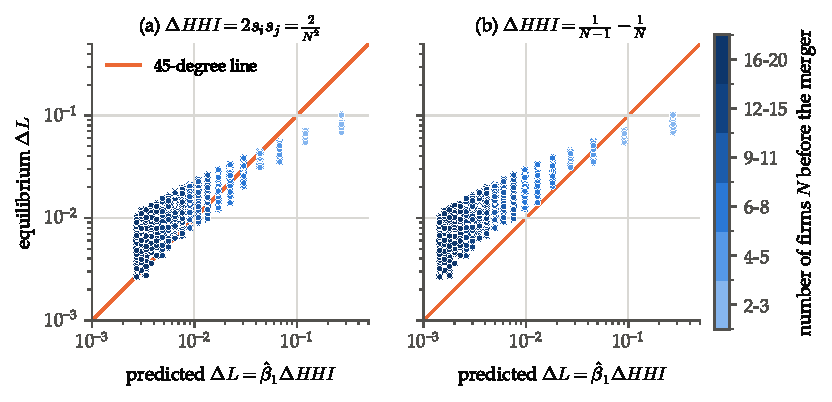
\includegraphics[width=\textwidth]{figures/appC/merger_mc.pdf}
\caption{Equilibrium against predicted changes in the Lerner index after a merger of two firms in 954
simulated Cournot industries, on logarithmic axes. Predictions multiply the cross-industry slope
$\hat\beta_1 = 0.546$ by the share-based change in concentration (panel a) or by the equilibrium change (panel b).
Colours group industries by the number of firms before the merger. Points above the orange line are mergers
whose effect the regression understates.}
\label{fig:C-merger-mc}
\end{figure}

Three findings stand out. First, the regression gets the direction of the error wrong in a systematic way.
For concentrated industries ($N \le 4$) it overstates the effect of a merger by a factor of about two. For
unconcentrated industries ($N \ge 11$) it understates the effect, and with the equilibrium $\Delta\HHI$ the
prediction is less than a third of the truth. The reason is concavity. The OLS slope 0.546 is a
variance-weighted average of chord slopes, and most of the variation in $\HHI$ comes from concentrated
industries, where the Cournot curve is flat. The local slope averages 1.452 across the 1,000 industries, and it
is largest where $\HHI$ is small.

Second, the share-based formula appears to do better than the equilibrium change in concentration. Overall,
its prediction errs by more than 50 percent in 33 percent of industries, against 71 percent for the equilibrium
version. This is an accident of offsetting errors. The share-based formula overstates the change in
concentration by the factor $\frac{2(N - 1)}{N}$, close to two in unconcentrated industries, and this offsets
part of the slope's understatement there. A correct input combined with a wrong slope produces a worse
prediction.

Third, the error comes from the common slope, and the linear approximation does little harm. The local-slope
benchmark misses by more than
50 percent in only 5.5 percent of industries, all of them concentrated. Its remaining error comes from
concavity, since the tangent at the pre-merger point is steeper than the chord to the post-merger point, so it
overpredicts in every industry. The high correlations in Panel B reflect the fact that predicted and actual
effects both fall with $N$. They say little about accuracy, since every prediction uses the same slope for all
industries.

\subsection{Computational notes}\label{sec:C-cournot-computation}

The script \texttt{figures/appC/src/cournot\_merger\_mc.py} implements part (i) in the following steps.
\begin{enumerate}
\item Draw $(a, c, b, \ln F)$ in batches from the stated uniform distributions with a fixed seed. Keep draws with
  $x \ge 2$ until 1,000 industries are accepted, then draw $N$ for each industry.
\item Compute $L = \frac{a - c}{a + Nc}$ and $\HHI = \frac{1}{N}$.
\item Run OLS of $L$ on $(1, \HHI)$. Compute HC1 standard errors as the square roots of the diagonal of
  $\frac{n}{n - 2}(X^\top X)^{-1}\big(\sum_k \hat e_k^2 x_kx_k^\top\big)(X^\top X)^{-1}$ (\cref{app:econometrics}).
\item For industries with $N \ge 2$, compute $\Delta L$ from \eqref{eq:C-merger-dL} and the three predictions,
  then summarize by groups of $N$.
\end{enumerate}

\section{What tax pass-through reveals about conduct}\label{sec:C-passthrough}

The first problem showed that the cross-section of margins and concentration cannot reveal conduct. This problem
turns to a source of variation inside one industry, a shock to cost. Excise taxes are a part of marginal cost that
the econometrician observes without any cost data. \citet{Sumner1981} used this fact to test for monopoly pricing in the US cigarette industry. He found that cigarette
prices rose by more than state excise taxes, and he concluded that the industry was neither competitive nor an
effective cartel. This problem derives what a pass-through rate can and cannot reveal about conduct. It checks the
numbers in Sumner's main table and re-estimates his regression on a reconstructed panel. It then adds clustered
inference with a power calculation, a test of constant pass-through, ad valorem taxes, and a way to recover
marginal cost from two kinds of taxes. \Cref{sec:03-sumner} treats the paper as a case study, and
\cref{sec:02-passthrough} develops the theory of pass-through. Here we work through every step on the data.

\subsection{Statement}\label{sec:C-passthrough-statement}

A homogeneous good has twice differentiable inverse demand $P(Q)$ with $P'(Q) < 0$. The \emph{curvature} of inverse
demand is $\chi \equiv -\frac{QP''(Q)}{P'(Q)}$, and the market elasticity is $\varepsilon = -\frac{P}{QP'(Q)} > 0$.
Sellers pay a specific tax $t$ per unit and have marginal cost $c$, constant unless stated otherwise. Industry
conduct is a constant $\theta \in [0, 1]$, and the equilibrium satisfies the supply relation
\begin{equation}\label{eq:C-supply-tax}
P(Q) + \theta QP'(Q) = c + t .
\end{equation}
Competition is $\theta = 0$, monopoly is $\theta = 1$, and symmetric Cournot with $N$ firms is $\theta = \frac{1}{N}$
(\cref{cor:03-benchmarks}). \emph{Pass-through} is $\rho \equiv \frac{\dd P}{\dd t}$, the change in the equilibrium
price per unit of tax.

The data form a balanced state-year panel reconstructed from the historical volume of \emph{The Tax Burden on
Tobacco} (1983, Table 13). It covers 47 states and the District of Columbia annually from 1954 to 1978, a
total of 1,200 observations. Alaska, Hawaii and New Hampshire are excluded. For state $s$ and year $y$, $p_{sy}$ is
the weighted-average retail price per pack and $t_{sy}$ is the combined state and federal excise tax, both in nominal
cents. Both are recorded on November 1 of each year. Municipal taxes are excluded, and the federal tax is 8 cents per
pack throughout. The national consumer price index $CPI_y$ (CPI-U, 1982--84 average equal to 100) deflates prices to
$P_{sy} = \frac{100\,p_{sy}}{CPI_y}$ and taxes to $T_{sy} = \frac{100\,t_{sy}}{CPI_y}$. \Cref{tab:C-panel-stats}
summarizes the panel.

\begin{table}[htbp]
\centering
\begin{threeparttable}
\caption{The state-year cigarette panel, 1954--1978}
\label{tab:C-panel-stats}
\small
\begin{tabular}{@{}lrrrrrr@{}}
\toprule
Variable & Mean & S.d. & Min & Max & Mean 1954 & Mean 1978 \\
\midrule
Retail price $p_{sy}$ (cents per pack) & 34.04 & 10.51 & 18.20 & 66.50 & 22.45 & 56.55 \\
Excise tax $t_{sy}$ (cents per pack) & 15.73 & 4.66 & 8.00 & 29.00 & 11.10 & 20.63 \\
Real price $P_{sy}$ (1982--84 cents) & 90.67 & 9.65 & 64.32 & 126.67 & 83.47 & 86.74 \\
Real tax $T_{sy}$ (1982--84 cents) & 42.73 & 8.92 & 15.34 & 71.60 & 41.28 & 31.64 \\
Tax share $\frac{t_{sy}}{p_{sy}}$ & 0.467 & 0.060 & 0.229 & 0.584 & 0.492 & 0.361 \\
\bottomrule
\end{tabular}
\begin{tablenotes}\footnotesize
\item Notes: 1,200 state-years (47 states and the District of Columbia). The tax is the state excise tax plus the
federal tax of 8 cents. The CPI-U is 26.9 in 1954 and 65.2 in 1978. The median state tax rises from 3 cents in 1954
to 12 cents in 1978, as \citet[n.~8]{Sumner1981} reports, and the mean tax share is close to his 48.7 and 35.5
percent. Of the 1,152 year-to-year transitions within states, 191 involve a tax change, 6 of them decreases, and the
mean change is 2.39 cents. The real tax falls over the sample, as Sumner notes. Source:
\texttt{figures/appC/src/sumner\_passthrough.py}.
\end{tablenotes}
\end{threeparttable}
\end{table}

\begin{enumerate}[label=(\alph*)]
\item Derive the pass-through rate from \eqref{eq:C-supply-tax}, first with constant marginal cost and then with
  marginal cost $c(Q)$ rising in output. What does $\rho > 1$ imply?
\item Show that one pass-through rate identifies only the composite $\kappa \equiv \theta(\chi - 1)$. Work out the
  linear, log, constant-elasticity and symmetric Cournot cases.
\item Sumner writes the price of firm $j$ as $P_j = \frac{\eta_j}{\eta_j + 1}M_j$, where $\eta_j < 0$ is the
  elasticity of the firm's demand and $M_j = X_j\phi + E_j + t$ its marginal cost. He estimates
  $p_{sy} = X_{sy}\psi + \Theta t_{sy} + U_{sy}$. Derive this aggregate equation and the elasticity implied by
  $\Theta$, and check the elasticities he reports.
\item Estimate $p_{sy} = \mu_s + \tau_y + \rho\,t_{sy} + e_{sy}$ with conventional and state-clustered standard errors.
  Test $\rho = 1$ and assess the power of the test.
\item Re-estimate the regression in real terms. Explain why deflating changes the estimate even though the
  regression contains year effects.
\item Let pass-through vary with the real tax and test whether it does.
\item Describe the set of pairs $(\chi, \theta)$ consistent with the estimate.
\item Derive a bound on $\theta$ from the levels of prices and taxes that does not depend on curvature, and
  evaluate it.
\item Show how changes in the mix of brands affect the pass-through of an average price.
\item Derive the pass-through of an ad valorem tax at rate $\tau$ on the consumer price.
\item What additional data would identify $\theta$?
\end{enumerate}

\subsection{Solution}\label{sec:C-passthrough-solution}

\casehead{Part (a)}
We write equilibrium output as a function $Q(t)$ of the tax and differentiate the supply relation. The general
result allows marginal cost $c(Q)$ to rise with output.

\begin{proposition}[Pass-through of a specific tax]\label{prop:C-passthrough}
Replace $c$ by a differentiable marginal cost $c(Q)$ with $c'(Q) \ge 0$ in \eqref{eq:C-supply-tax}. Suppose the
equilibrium is interior and stable, in the sense that $D \equiv (1 + \theta)P' + \theta QP'' - c' < 0$. Then
\begin{equation}\label{eq:C-rho-general}
\rho = \frac{1}{1 + \theta(1 - \chi) + \frac{c'(Q)}{\lvert P'(Q)\rvert}} ,
\end{equation}
and the denominator is positive. With constant marginal cost,
\begin{equation}\label{eq:C-rho-flat}
\rho = \frac{1}{1 + \theta(1 - \chi)} .
\end{equation}
\end{proposition}

\begin{proof}
This is the first form of \cref{prop:03-passthrough}, with $c$ in place of $MC$ and $D$ in place of $J$. Steps 1 to 3
of the proof of \cref{prop:02-pt-general} derive it by differentiating the supply relation with respect to $t$.
Setting $c' = 0$ gives \eqref{eq:C-rho-flat}.
\end{proof}

\Cref{prop:03-passthrough} also gives the elasticity form of \citet{WeylFabinger2013}. Three consequences follow. First, competition with constant marginal cost
($\theta = 0$, $c' = 0$) gives $\rho = 1$ for every demand curve, because price equals marginal cost. Second,
competition with rising marginal cost gives $\rho = \frac{1}{1 + \frac{c'}{\lvert P'\rvert}} < 1$. Sellers bear part
of the tax, because their marginal cost falls as output contracts. Third, for any conduct a steeper marginal cost
curve lowers $\rho$. Hence $\rho \le 1$ under competition whatever the shapes of demand and cost. An estimate
significantly above one rejects competition without any assumption on curvature, which is the robust half of
Sumner's test.

The denominator of \eqref{eq:C-rho-flat} has a simple reading. Perceived marginal revenue is $P + \theta QP'$, and
its slope relative to the slope of demand is
\begin{equation*}
\frac{(1 + \theta)P' + \theta QP''}{P'} = 1 + \theta(1 - \chi) .
\end{equation*}
A tax raises effective cost by $t$, and output falls until perceived marginal revenue has risen by $t$. The price
rises by more than the tax when perceived marginal revenue is flatter than demand, that is, when $\theta > 0$ and
$\chi > 1$.

\casehead{Part (b)}
With constant marginal cost, \eqref{eq:C-rho-flat} rearranges to
\begin{equation}\label{eq:C-kappa}
\frac{1}{\rho} = 1 + \theta(1 - \chi)
\qquad\Longleftrightarrow\qquad
\kappa \equiv \theta(\chi - 1) = 1 - \frac{1}{\rho} .
\end{equation}
The data enter only through $\rho$, and $\rho$ depends on conduct and curvature only through $\kappa$. Every pair on
the hyperbola $\theta(\chi - 1) = \kappa$ generates the same pass-through. If $\rho > 1$, then $\kappa > 0$, and any
$\theta > 0$ fits the data with curvature $\chi = 1 + \frac{\kappa}{\theta}$. Pass-through alone can therefore reject
competition but never monopoly (\cref{prop:03-passthrough-id}).

Four special cases show how curvature disciplines the reading, and \cref{tab:C-curvature} collects them. For
\emph{linear demand} $P = a - bQ$, $P'' = 0$, so $\chi = 0$ and $\rho = \frac{1}{1 + \theta} \le 1$. For \emph{log
demand} $P = a_0 - b_0\ln Q$ with $b_0 > 0$, the derivatives are $P' = -\frac{b_0}{Q}$ and $P'' = \frac{b_0}{Q^2}$.
Hence
\begin{equation*}
\chi = -\frac{Q\cdot\frac{b_0}{Q^2}}{-\frac{b_0}{Q}} = 1 , \qquad \rho = 1 \text{ for every } \theta .
\end{equation*}
The supply relation becomes $P - \theta b_0 = c + t$, a constant dollar markup. For \emph{constant-elasticity demand}
$P = AQ^{-\frac{1}{\varepsilon}}$,
\begin{equation*}
P' = -\frac{1}{\varepsilon}AQ^{-\frac{1}{\varepsilon} - 1}, \qquad
P'' = \frac{1}{\varepsilon}\Big(1 + \frac{1}{\varepsilon}\Big)AQ^{-\frac{1}{\varepsilon} - 2}, \qquad
\chi = -\frac{QP''}{P'} = 1 + \frac{1}{\varepsilon} .
\end{equation*}
Then $1 + \theta(1 - \chi) = 1 - \frac{\theta}{\varepsilon}$, so that
\begin{equation}\label{eq:C-rho-ce}
\rho = \frac{\varepsilon}{\varepsilon - \theta}, \qquad \kappa = \frac{\theta}{\varepsilon}, \qquad
\theta = \varepsilon\kappa .
\end{equation}
For \emph{symmetric Cournot} with $N$ firms and any demand, $\theta = \frac{1}{N}$ gives
$\rho = \frac{1}{1 + \frac{1 - \chi}{N}} = \frac{N}{N + 1 - \chi}$, and a given $\kappa$ requires $\chi = 1 + N\kappa$.

\begin{table}[htbp]
\centering
\begin{threeparttable}
\caption{Curvature, pass-through and the reading of an estimate above one}
\label{tab:C-curvature}
\small
\begin{tabular}{@{}llccl@{}}
\toprule
Demand and conduct & Inverse demand & $\chi$ & $\rho$ & Reading of $\hat\rho = 1.075$ \\
\midrule
Linear, conduct $\theta$ & $a - bQ$ & 0 & $\frac{1}{1 + \theta}$ & impossible, since $\rho \le 1$ \\
\addlinespace
Log, conduct $\theta$ & $a_0 - b_0\ln Q$ & 1 & 1 & impossible, since $\rho = 1$ \\
\addlinespace
Constant elasticity, conduct $\theta$ & $AQ^{-\frac{1}{\varepsilon}}$ & $1 + \frac{1}{\varepsilon}$ &
  $\frac{\varepsilon}{\varepsilon - \theta}$ & $\theta = 0.069\,\varepsilon$ \\
\addlinespace
Any, symmetric Cournot & $P(Q)$, $\theta = \frac{1}{N}$ & $\chi$ & $\frac{N}{N + 1 - \chi}$ & $\chi = 1 + 0.069N$ \\
\addlinespace
Any, monopoly & $P(Q)$, $\theta = 1$ & $\chi$ & $\frac{1}{2 - \chi}$ & $\chi = 1.069$ \\
\bottomrule
\end{tabular}
\begin{tablenotes}\footnotesize
\item Notes: Constant marginal cost. The last column uses $\hat\kappa = 1 - \frac{1}{\hat\rho} = 0.069$ from
specification M0 in part (d). Linear and constant-elasticity demand belong to the power family
$P = a_0 - b_0Q^{\gamma}$, whose curvature $\chi = 1 - \gamma$ is constant, and log demand is its limit as
$\gamma \to 0$ (\cref{ex:02-pt-examples}).
\end{tablenotes}
\end{threeparttable}
\end{table}

The monopoly row connects to \citet{BulowPfleiderer1983}. A monopolist with constant marginal cost passes through
less than one if and only if direct demand is log-concave (\cref{cor:02-bulow-pfleiderer}). An estimate above one,
read as monopoly, therefore requires log-convex demand at the observed prices. Constant elasticity is one such
demand curve, and it is the one Sumner assumes.

\casehead{Part (c)}
\citet[p.~1011]{Sumner1981} starts from the markup rule of firm $j$,
\begin{equation}\label{eq:C-sumner1}
P_j = \frac{\eta_j}{\eta_j + 1}\,M_j \equiv \Theta_jM_j \qquad \text{(his eq.~1)},
\end{equation}
where $\eta_j < 0$ is the elasticity of the demand curve facing firm $j$ (his sign convention). The marginal cost of
firm $j$ is $M_j$. Under monopoly $\eta_j$ is the market elasticity. Under perfect competition $\eta_j = -\infty$ and
the price-cost ratio $\Theta_j$ equals one. Marginal cost is
\begin{equation}\label{eq:C-sumner2}
M_j = X_j\phi + E_j + t \qquad \text{(his eq.~2)},
\end{equation}
with observed cost factors $X_j$, unobserved factors $E_j$ and the tax $t$, which is common to all firms. Sumner
writes $\beta$, $\epsilon_j$, $R$ and $\theta$ where we write $\phi$, $E_j$, $t$ and $\Theta$, and we rename them to
avoid clashes with the book's notation.

Only state-average prices are observed, so Sumner aggregates (p.~1012). Let $S_j$ be firm $j$'s market share, and
define the share-weighted averages $P = \sum_j S_jP_j$, $M = \sum_j S_jM_j$ and $\Theta = \sum_j S_j\Theta_j$. Writing
each firm's terms as deviations from the averages,
\begin{align*}
P = \sum_j S_j\Theta_jM_j
&= \sum_j S_j\big[\Theta + (\Theta_j - \Theta)\big]\big[M + (M_j - M)\big] \\
&= \Theta M + \Theta\sum_j S_j(M_j - M) + M\sum_j S_j(\Theta_j - \Theta) + \sum_j S_j(\Theta_j - \Theta)(M_j - M) \\
&= \Theta M + \sum_j S_j(\Theta_j - \Theta)(M_j - M) .
\end{align*}
The two middle sums vanish because the shares sum to one and $\Theta$ and $M$ are share-weighted means. The last line
is his eq.~3. The remaining sum is the share-weighted covariance of price-cost ratios and marginal costs. Sumner drops
it under any of three conditions. Elasticities vary little across firms, marginal costs vary little, or the two are
nearly unrelated. He supports the approximation with two facts: retail prices vary little across brands within a
market, and all brands are made in one region with a standard technology. He also writes $\Theta = \frac{\eta}{\eta + 1}$
for the share-weighted elasticity $\eta = \sum_j S_j\eta_j$. This step is exact only when all firms face the same
elasticity, because the map from $\eta_j$ to $\Theta_j$ is nonlinear.

Dropping the covariance and substituting \eqref{eq:C-sumner2} gives $P = \Theta(X\phi + E + t)$. In panel form,
\begin{equation}\label{eq:C-sumner4}
p_{sy} = X_{sy}\psi + \Theta\,t_{sy} + U_{sy}, \qquad \psi = \Theta\phi, \quad U_{sy} = \Theta E_{sy}
\qquad \text{(his eq.~4)} .
\end{equation}
The tax coefficient is the price-cost ratio. Competition implies $\Theta = 1$, and any market power implies
$\Theta > 1$. To recover the firm-level elasticity, we invert $\Theta = \frac{\eta}{\eta + 1}$:
\begin{align*}
\Theta(\eta + 1) &= \eta , \\
\eta(\Theta - 1) &= -\Theta , \\
\eta &= \frac{\Theta}{1 - \Theta} .
\end{align*}
Equivalently, the Lerner index of the firms is $\frac{P - M}{P} = 1 - \frac{1}{\Theta} = -\frac{1}{\eta}$.

\Cref{tab:C-sumner1} reproduces Sumner's Table 1 (p.~1017) and adds the implied quantities. The printed
elasticities equal $\frac{1}{1 - \hat\Theta}$ to the reported precision. Since
$\frac{1}{1 - \Theta} = \frac{\Theta}{1 - \Theta} + 1 = \eta + 1$, each printed value is one unit smaller in absolute
value than the exact inversion. The printed figure inverts the markup over cost, $\frac{P - M}{M} = \Theta - 1 =
-\frac{1}{\eta + 1}$, in place of the Lerner index. The two inversions agree to first order in $\Theta - 1$, and the
gap of 3 to 7 percent leaves Sumner's conclusions unchanged. His conclusion uses the same approximation. With
$\Theta = 1.05$, a 1 percent price increase lowers a firm's sales by 20 percent (p.~1019), where the exact inversion
gives 21 percent.

\begin{table}[htbp]
\centering
\begin{threeparttable}
\caption{Sumner's estimates of the tax coefficient and what they imply}
\label{tab:C-sumner1}
\small
\setlength{\tabcolsep}{4.5pt}
\begin{tabular}{@{}lcccccccc@{}}
\toprule
 & \multicolumn{3}{c}{Sumner (1981), Table 1} & \multicolumn{4}{c}{Implied by $\hat\Theta$} & Replication \\
\cmidrule(lr){2-4}\cmidrule(lr){5-8}\cmidrule(l){9-9}
Row & $\hat\Theta$ & S.e. & $\eta$ printed & $t$ for $\Theta = 1$ & $\frac{1}{1 - \hat\Theta}$ &
  $\frac{\hat\Theta}{1 - \hat\Theta}$ & $1 - \frac{1}{\hat\Theta}$ & $\hat\Theta$ (s.e.) \\
\midrule
(1) Dummies, OLS & 1.074 & 0.013 & $-13.5$ & 5.7 & $-13.5$ & $-14.5$ & 0.069 & 1.075 (0.013) \\
(2) CPI, OLS & 1.029 & 0.011 & $-34.5$ & 2.6 & $-34.5$ & $-35.5$ & 0.028 & 1.029 (0.011) \\
(3) CPI, VC & 1.069 & 0.013 & $-14.5$ & 5.3 & $-14.5$ & $-15.5$ & 0.065 & 1.069 (0.013) \\
\bottomrule
\end{tabular}
\begin{tablenotes}\footnotesize
\item Notes: Dependent variable: retail price per pack in cents, 1,200 state-years. Row (1) includes a dummy for each
year (1978 excluded) and each state (Wyoming excluded). Rows (2) and (3) include the national consumer price index and
no dummies. VC is a variance-components GLS estimator with random state and year effects \citep{FullerBattese1974}.
Sumner reports $R^2$ of about 0.99 with dummies and about 0.95 without. ``$\eta$ printed'' is his implied price
elasticity, with his negative sign. The next four columns are computed from his printed $\hat\Theta$, and
$1 - \frac{1}{\hat\Theta}$ is the implied Lerner index. The replication uses the reconstructed panel with
conventional standard errors, as in the paper, and gives $R^2$ of 0.994 for row (1) and 0.985 for row (2).
\end{tablenotes}
\end{threeparttable}
\end{table}

Sumner reports two further checks. First, he lets the price-cost ratio vary with the price,
$\Theta(P) = \gamma_SP^{1 - \lambda_S}$, where $\gamma_S$ and $\lambda_S$ are his $\gamma$ and $\lambda$ (n.~7). The
markup rule $P = \Theta(P)M$ then gives
\begin{equation*}
P = \gamma_SP^{1 - \lambda_S}M
\qquad\Longrightarrow\qquad
P^{\lambda_S} = \gamma_SM
\qquad\Longrightarrow\qquad
P = (\gamma_SM)^{\frac{1}{\lambda_S}} .
\end{equation*}
Substituting \eqref{eq:C-sumner2} and adding an additive or a multiplicative error gives his eqs.~4$'$ and 4$''$,
which he estimates by nonlinear least squares. The value $\lambda_S = 1$ restores a constant ratio
$\Theta = \gamma_S$. The estimates are $\hat\lambda_S = 0.972$ (0.027) and 0.981 (0.026), with
$\hat\gamma_S = 1.029$ and 1.062 (n.~9). The $t$-statistics for $\lambda_S = 1$ are 1.04 and 0.73, so constancy is
not rejected. Second, the pooled equation estimated year by year gives estimates in the range of Table 1 with no
trend. A squared tax term added to the yearly equations is insignificant in most years.

Sumner reads the results in two steps (pp.~1016--1017). Estimates significantly above one reject atomistic competition. The
implied firm elasticities are 13.5 to 34.5 in absolute value. They are far above estimates of the industry elasticity,
which are ``generally between $-0.3$ and $-0.8$.'' His own estimate is about $-0.40$ (n.~10). A cartel would face the
industry elasticity, so he rejects an effective cartel. He adds that with $\Theta = 1.05$ and prices 5 percent above
marginal cost, market power raises the average price by about 3 cents per pack (p.~1019).

The conduct model of part (b) gives Sumner's ratio a structural meaning. With constant-elasticity demand and flat
cost, the Lerner form of \eqref{eq:C-supply-tax} is $\frac{P - c - t}{P} = \frac{\theta}{\varepsilon}$, so
\begin{equation*}
P = \frac{\varepsilon}{\varepsilon - \theta}(c + t), \qquad
\Theta = \frac{\varepsilon}{\varepsilon - \theta} = \rho, \qquad
\eta = \frac{\Theta}{1 - \Theta} = -\frac{\varepsilon}{\theta} .
\end{equation*}
Sumner's firm elasticity is the market elasticity divided by conduct, and his Lerner index $1 - \frac{1}{\Theta}$
equals $\frac{\theta}{\varepsilon} = \kappa$. Without constant elasticity, $\Theta$ is the pass-through $\rho$ but no
longer the price-cost ratio, and the two must be kept apart.

\casehead{Part (d)}
We call Sumner's row (1) specification M0:
\begin{equation}\label{eq:C-M0}
p_{sy} = \mu_s + \tau_y + \rho\,t_{sy} + e_{sy} .
\end{equation}
The state effects $\mu_s$ absorb stable differences in non-tax costs and demand. The year effects $\tau_y$ absorb
national movements in costs and in the price level. Under \eqref{eq:C-sumner4} they absorb $\Theta X_{sy}\phi$ when
non-tax cost is additive in a state and a year component. Identification requires that tax changes within a state,
relative to other states in the same year, be unrelated to shocks to cost and demand. Formally,
$\E[e_{sy} \mid t_{s1}, \dots, t_{sY}] = 0$ for every state, after conditioning on the fixed effects
(\cref{sec:03-sumner-design}).

By the Frisch-Waugh-Lovell theorem, OLS with both sets of dummies equals the regression of $p_{sy}$ on the
two-way demeaned tax. In a balanced panel the demeaned tax is
\begin{equation*}
\tilde t_{sy} = t_{sy} - \bar t_{s\cdot} - \bar t_{\cdot y} + \bar t_{\cdot\cdot} ,
\end{equation*}
where $\bar t_{s\cdot}$, $\bar t_{\cdot y}$ and $\bar t_{\cdot\cdot}$ are the state means, the year means and the
grand mean. Then
\begin{equation}\label{eq:C-fwl}
\hat\rho = \frac{\sum_{s,y}\tilde t_{sy}p_{sy}}{\sum_{s,y}\tilde t_{sy}^2}, \qquad
\hat\rho - \rho = \frac{\sum_{s,y}\tilde t_{sy}e_{sy}}{\sum_{s,y}\tilde t_{sy}^2} .
\end{equation}
The conventional variance estimator assumes independent errors with a common variance,
\begin{equation*}
\hat V_{\text{conv}} = \frac{s^2}{\sum_{s,y}\tilde t_{sy}^2}, \qquad s^2 = \frac{1}{N - K}\sum_{s,y}\hat e_{sy}^2 ,
\end{equation*}
with $N = 1{,}200$ and $K = 73$ coefficients (the tax, 48 state effects and 24 year effects). The cluster-robust
estimator allows any correlation among the errors of one state:
\begin{equation}\label{eq:C-vcl}
\hat V_{\text{cl}} = \frac{G}{G - 1}\cdot\frac{N - 1}{N - K}\cdot
\frac{\sum_s\big(\sum_y\tilde t_{sy}\hat e_{sy}\big)^2}{\big(\sum_{s,y}\tilde t_{sy}^2\big)^2} ,
\end{equation}
with $G = 48$ clusters. Inference uses the $t$ distribution with $G - 1 = 47$ degrees of freedom, whose 97.5 percent
quantile is 2.012 (\cref{app:econometrics}).

\Cref{tab:C-passthrough} reports the estimates. M0 gives $\hat\rho = 1.0746$ with a conventional standard error of
0.0132, which reproduces Sumner's 1.074 (0.013). The $t$-statistic for $\rho = 1$ is 5.64. The clustered standard
error is 0.0340, 2.57 times the conventional one. The $t$-statistic falls to 2.19, with $p = 0.033$ and a 95 percent
interval of $[1.006, 1.143]$. The rejection of competition survives clustering, but by a much thinner margin. Our
replications of Sumner's rows (2) and (3) give 1.029 (0.011) and 1.069 (0.013), equal to his estimates.

\begin{table}[htbp]
\centering
\begin{threeparttable}
\caption{Pass-through regressions on the reconstructed panel}
\label{tab:C-passthrough}
\small
\begin{tabular}{@{}lcccc@{}}
\toprule
Specification & Estimate & S.e. & 95\% interval & $p$ for $\rho = 1$ \\
\midrule
\multicolumn{5}{@{}l}{\emph{Panel A. Nominal cents}} \\
M0: state and year effects, conventional s.e. & 1.075 & 0.013 & $[1.049,\ 1.101]$ & $<0.001$ \\
M0: state and year effects, clustered s.e. & 1.075 & 0.034 & $[1.006,\ 1.143]$ & 0.033 \\
National CPI, OLS, conventional s.e. & 1.029 & 0.011 & $[1.008,\ 1.050]$ & 0.007 \\
National CPI, variance components & 1.069 & 0.013 & $[1.044,\ 1.093]$ & $<0.001$ \\
\addlinespace
\multicolumn{5}{@{}l}{\emph{Panel B. Real cents, state and year effects, clustered s.e.}} \\
M1 & 1.107 & 0.026 & $[1.055,\ 1.158]$ & $<0.001$ \\
Nominal, CPI-scaled state effects, unweighted & 1.102 & 0.026 & $[1.050,\ 1.155]$ & $<0.001$ \\
\addlinespace
\multicolumn{5}{@{}l}{\emph{Panel C. Pass-through varying with the real tax (M2), clustered s.e.}} \\
$\rho(T)$ at the 10th percentile, $T = 29.9$ & 1.097 & 0.039 & $[1.018,\ 1.176]$ & 0.017 \\
$\rho(T)$ at the median, $T = 43.8$ & 1.106 & 0.025 & $[1.055,\ 1.157]$ & $<0.001$ \\
$\rho(T)$ at the 90th percentile, $T = 53.5$ & 1.113 & 0.034 & $[1.044,\ 1.181]$ & 0.002 \\
$\rho(p_{90}) - \rho(p_{10})$ & 0.016 & 0.053 & $[-0.090,\ 0.122]$ & \\
\addlinespace
\multicolumn{5}{@{}l}{\emph{Panel D. Composite identified by pass-through (clustered M0)}} \\
$\hat\kappa = 1 - \frac{1}{\hat\rho}$ & 0.069 & & $[0.006,\ 0.125]$ & \\
\bottomrule
\end{tabular}
\begin{tablenotes}\footnotesize
\item Notes: 1,200 state-years. Clustered standard errors allow correlation within states (48 clusters), and their
intervals and $p$-values use the $t$ distribution with 47 degrees of freedom. Conventional intervals use $N - K$
degrees of freedom, and the variance-components row uses the normal distribution. In M2 the test of $b_2 = 0$ has
$p = 0.76$. The interval for $\kappa$ maps the endpoints of the clustered interval for $\rho$. The CPI-scaled row
differs from M1 only in its weights (\cref{lem:C-deflate}). Source: \texttt{figures/appC/src/sumner\_passthrough.py}.
\end{tablenotes}
\end{threeparttable}
\end{table}

Clustering matters because both the errors and the regressor are persistent within states. The pooled first-order
autocorrelation of the M0 residuals within states is $r_e = 0.64$, and that of the demeaned tax is $r_x = 0.85$.
Taxes change rarely. Of the 1,152 year-to-year transitions within states, 191 involve a tax change, and only 6 of
those are decreases. A standard approximation shows the size of the problem. Suppose that, within a state, the
errors are AR(1) with coefficient $r_e$ and the sample autocorrelation of $\tilde t$ at lag $k$ is close to $r_x^k$.
Then
\begin{equation*}
\Var\Big(\sum_y\tilde t_{sy}e_{sy}\Big)
= \sigma_e^2\sum_{y,y'}\tilde t_{sy}\tilde t_{sy'}r_e^{\lvert y - y'\rvert}
\approx \sigma_e^2\sum_y\tilde t_{sy}^2\Big(1 + 2\sum_{k \ge 1}r_x^kr_e^k\Big)
= \sigma_e^2\sum_y\tilde t_{sy}^2\cdot\frac{1 + r_xr_e}{1 - r_xr_e} .
\end{equation*}
The conventional formula omits the last factor. Its square root is
$\sqrt{\frac{1 + r_xr_e}{1 - r_xr_e}} = 1.83$, with $r_xr_e = 0.848\times0.638 = 0.541$. The cluster-robust ratio of 2.57 is larger, because
the approximation imposes a common geometric decay that the data need not follow. Both numbers say that Sumner's
standard error is too small by a factor of about two or more \citep{BertrandDufloMullainathan2004}.

The power of the clustered test is modest. A two-sided 5 percent test has 80 percent power against deviations from
one of at least $(t_{0.975, 47} + t_{0.80, 47})\times 0.034 = (2.012 + 0.849)\times0.034 = 0.097$. With the
conventional standard error the threshold would be 0.038. The estimated deviation of 0.075 lies below the clustered
threshold. If the true pass-through were 1.075, a test on a new sample of the same size would reject competition
with probability 0.57. The rejection in our sample is evidence against competition, but a replication could easily
have failed to reject.

\casehead{Part (e)}
Specification M1 replaces nominal by real cents:
\begin{equation}\label{eq:C-M1}
P_{sy} = \mu_s + \tau_y + \rho\,T_{sy} + e_{sy} .
\end{equation}
It gives $\hat\rho = 1.107$ with a clustered standard error of 0.026, a 95 percent interval of $[1.055, 1.158]$
and $p < 0.001$ for $\rho = 1$. The estimate is 0.032 higher than in M0. Year effects absorb any common change in the
price level, so the difference needs an explanation.

\begin{lemma}[Deflating a two-way fixed-effects regression]\label{lem:C-deflate}
OLS estimation of \eqref{eq:C-M1} gives the same $\hat\rho$ as weighted least squares estimation of the nominal
equation
\begin{equation*}
p_{sy} = \mu_s\frac{CPI_y}{100} + \tau'_y + \rho\,t_{sy} + u_{sy}
\end{equation*}
with weights $\big(\frac{100}{CPI_y}\big)^2$, where $\tau'_y$ are unrestricted year effects.
\end{lemma}

\begin{proof}
Multiply \eqref{eq:C-M1} by $\frac{CPI_y}{100}$. Since $P_{sy}\frac{CPI_y}{100} = p_{sy}$ and
$T_{sy}\frac{CPI_y}{100} = t_{sy}$,
\begin{equation*}
p_{sy} = \mu_s\frac{CPI_y}{100} + \tau_y\frac{CPI_y}{100} + \rho\,t_{sy} + e_{sy}\frac{CPI_y}{100} .
\end{equation*}
The second term varies only by year, so it is an unrestricted year effect $\tau'_y$. The error is
$u_{sy} = e_{sy}\frac{CPI_y}{100}$. OLS on \eqref{eq:C-M1} minimizes
$\sum_{s,y}e_{sy}^2 = \sum_{s,y}\big(\frac{100}{CPI_y}\big)^2u_{sy}^2$, which is the weighted least squares
criterion for the nominal equation.
\end{proof}

Deflating therefore changes two things. First, the state effects become proportional to the price level. In nominal
terms the state differences in price net of tax grow with inflation, and this is a state-by-year interaction that
year effects cannot absorb. Second, observations from low-price years receive more weight. The CPI rises from 26.9 to
65.2 over the sample, so a 1954 observation has 5.9 times the weight of a 1978 observation. The script separates the
two channels. OLS on the nominal equation with CPI-scaled state effects and no weights gives 1.102 (0.026), and adding
the weights gives 1.107, identical to M1. Most of the change from 1.075 thus comes from the specification of the state
effects. If non-tax costs and margins in each state are fixed in real terms, M1 is the more natural specification.
Both specifications reject $\rho = 1$ at the 5 percent level.

\casehead{Part (f)}
Specification M2 adds a quadratic in the real tax:
\begin{equation}\label{eq:C-M2}
P_{sy} = \mu_s + \tau_y + b_1(T_{sy} - \bar T) + b_2(T_{sy} - \bar T)^2 + e_{sy} ,
\end{equation}
where $\bar T = 42.73$ is the sample mean of the real tax. Pass-through at tax level $T$ is the derivative
\begin{equation*}
\rho(T) = \frac{\partial P}{\partial T} = b_1 + 2b_2(T - \bar T) .
\end{equation*}
It is linear in $(b_1, b_2)$ with gradient $(1, 2(T - \bar T))$. Its variance is therefore
\begin{equation*}
\Var\big(\hat\rho(T)\big) = V_{11} + 4(T - \bar T)V_{12} + 4(T - \bar T)^2V_{22} ,
\end{equation*}
where $V$ is the clustered covariance matrix of $(\hat b_1, \hat b_2)$. The formula is exact here, and the delta
method gives the same expression (\cref{app:econometrics}).

The estimates are $\hat b_1 = 1.105$ (0.025) and $\hat b_2 = 0.00034$ (0.00112), and the test of $b_2 = 0$ gives
$p = 0.76$. Panel C of \cref{tab:C-passthrough} evaluates $\hat\rho(T)$ at three points of the tax distribution. It
is 1.097 (0.039) at the 10th percentile, 1.106 (0.025) at the median and 1.113 (0.034) at the 90th percentile. The
difference between the 90th and the 10th percentiles is $2\hat b_2(T_{90} - T_{10}) = 0.016$, with standard error
0.053 and 95 percent interval $[-0.090, 0.122]$. \Cref{fig:C-rho-T} plots $\hat\rho(T)$ with its confidence band.

\begin{figure}[htbp]
\centering
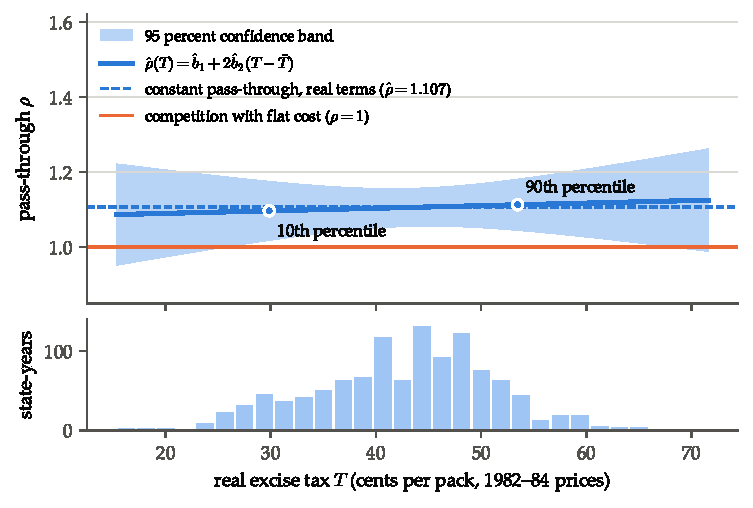
\includegraphics[width=0.86\textwidth]{figures/appC/rho_T.pdf}
\caption{Estimated pass-through as a function of the real excise tax, from specification M2, with a 95 percent
state-clustered confidence band. The dashed line is the constant pass-through of M1, and the orange line is the
competitive benchmark $\rho = 1$. The markers show the 10th and 90th percentiles of the real tax. The lower panel
shows the distribution of the real tax over the 1,200 state-years.}
\label{fig:C-rho-T}
\end{figure}

The data show no sign that pass-through varies with the tax, but the test has little power. With 80 percent power,
a 5 percent test would detect a difference between the two percentiles of $2.861\times0.053 = 0.151$ or more. This
threshold exceeds the estimated excess of pass-through over one in both M0 (0.075) and M1 (0.107). The band in \cref{fig:C-rho-T} also widens at the
extremes, where few state-years lie.

The quadratic also speaks to smuggling. Sumner argues that bootlegging would make the price a concave function of the
tax (n.~6). Bulk sales for shipment out of state lower measured prices in very low-tax states, and illegal
competition lowers them in very high-tax states. Concavity means $b_2 < 0$. Our estimate is positive and
insignificant, in line with his finding that squared tax terms are insignificant in most years.

A flat $\rho(T)$ would be weak evidence for constant-elasticity demand even with a precise estimate. Every member of
the power family in \cref{tab:C-curvature} has constant curvature, so with constant conduct its pass-through is the
same at every tax level. The test asks only whether $\kappa = \theta(\chi - 1)$ is stable over the observed range.
Sumner's estimates of $\lambda_S$ near one make the same point within his family, because $\lambda_S = 1$ makes the
price linear in the tax.

\casehead{Part (g)}
By \eqref{eq:C-kappa}, M0 identifies $\hat\kappa = 1 - \frac{1}{1.0746} = 0.069$. The map from $\rho$ to $\kappa$ is
increasing, so the clustered interval for $\rho$ maps into the interval $[0.006, 0.125]$ for $\kappa$. Every pair
$(\chi, \theta)$ on the hyperbola $\theta(\chi - 1) = 0.069$ fits the estimate equally well, and
\cref{fig:03-identified-set} draws this set with its band. Three points on it illustrate the range.
\begin{itemize}
\item Monopoly ($\theta = 1$) fits with $\chi = 1.069$, a demand curve slightly more convex than log demand.
\item Symmetric Cournot with six firms ($\theta = \frac{1}{6}$) fits with $\chi = 1 + 6\times0.069 = 1.42$.
\item Constant elasticity with an industry elasticity of 0.4 has $\chi = 3.5$. Then \eqref{eq:C-rho-ce} gives
  $\theta = 0.4\times0.069 = 0.028$, with interval $[0.002, 0.050]$. Elasticities of 0.3 and 0.8, the ends of the
  range Sumner quotes, give $\theta = 0.021$ and $0.056$.
\end{itemize}
Under constant elasticity with $\varepsilon = 0.4$, conduct of 0.028 matches symmetric Cournot with about 36 firms.
The industry is close to competitive under that reading. The data alone cannot choose among the three points, and
Sumner's rejection of collusion rests on the constant-elasticity assumption combined with outside estimates of the
elasticity. Even a precise $\hat\theta$ would measure market power only under the static model behind
\eqref{eq:C-supply-tax}. \citet{Corts1999} shows, analytically and by simulation, that the estimated conduct parameter
can badly mismeasure market power when firms sustain tacit collusion in a repeated game (abstract and Section~1). The
estimate need not even be positively correlated with the true elasticity-adjusted margin.

\casehead{Part (h)}
The level of prices and taxes gives a bound that needs no assumption on curvature. With constant marginal cost
$c \ge 0$, divide \eqref{eq:C-supply-tax} by $P$ and use $-\frac{QP'}{P} = \frac{1}{\varepsilon}$:
\begin{equation*}
\frac{P - c - t}{P} = \frac{\theta}{\varepsilon}
\qquad\Longrightarrow\qquad
\theta = \varepsilon\Big(1 - \frac{t}{P} - \frac{c}{P}\Big) \le \varepsilon\Big(1 - \frac{t}{P}\Big) .
\end{equation*}
This is \eqref{eq:03-lerner-bound}. The tax takes a large share of the cigarette price, so the bound is tight. With
$\varepsilon = 0.4$ it gives $\theta \le 0.4\times(1 - 0.467) = 0.213$ at the mean tax share and $\theta \le 0.308$ at
the lowest share in the sample (0.229). If $\theta$ and $\varepsilon$ are the same in every state-year, the highest
share (0.584) gives the tightest bound, $\theta \le 0.166$. Industry elasticities of 0.3 and 0.8 give bounds of 0.160
and 0.426 at the mean share. Every one of these bounds rules out monopoly whatever the curvature. Equivalently,
monopoly at the mean tax share requires an elasticity of at least $\frac{1}{1 - 0.467} = 1.88$ at the observed price,
and at the lowest share at least 1.30.

Under Sumner's constant-elasticity reading, in which $1 - \frac{1}{\rho}$ is the Lerner index (part (c)), the point
estimate also converts into cents. The value $1 - \frac{1}{\hat\rho} = 0.069$ applied to the mean price of 34.0 cents
gives a margin of price over marginal cost plus tax of 2.4 cents per pack. At the 1978 mean price
of 56.6 cents it gives 3.9 cents. Sumner's figure of about 3 cents uses $\Theta = 1.05$, and at the 1978 mean price
this ratio implies a margin of $56.6\times\big(1 - \frac{1}{1.05}\big) = 2.7$ cents.

\casehead{Part (i)}
Sumner's dependent variable is an average over brands. Suppose the measured price is $\bar p = \sum_j w_jp_j$ with
quantity weights $w_j$. Differentiating with respect to the tax,
\begin{equation}\label{eq:C-composition}
\frac{\dd\bar p}{\dd t} = \sum_j w_j\frac{\dd p_j}{\dd t} + \sum_j p_j\frac{\dd w_j}{\dd t} .
\end{equation}
The first term is the average of product-level pass-through, the object that conduct governs. The second is a
composition effect (\cref{rem:02-pt-composition}). A specific tax adds the same amount to every price, which is a
larger percentage of a cheap brand's price. Premium brands become relatively cheaper, consumers trade up, and the
composition term is positive. The regression then overstates product-level pass-through and leans toward rejecting
competition.

A back-of-the-envelope calculation shows how large the composition effect would have to be. Suppose packs come in
an economy and a premium tier whose prices differ by $\Delta$ cents. Suppose also that each price rises one for one
with the tax, as under competition with flat cost. The composition term is then $\Delta\frac{\dd w_H}{\dd t}$, where $w_H$ is
the premium share. Matching $\hat\rho = 1.075$ requires $\frac{\dd w_H}{\dd t} = \frac{0.075}{\Delta}$ per cent of
tax. With a hypothetical gap of $\Delta = 5$ cents, a 10-cent tax increase would have to raise the premium share by
15 percentage points. Two features of the data make shifts of this size unlikely. The Tobacco Tax Council's price
uses fixed national weights for the type of cigarette (regular, king, 100 mm) and the type of sale (carton, single
pack, machine). Shifts across these categories therefore do not move it \citep[p.~1016]{Sumner1981}. Sumner also reports
that retail prices vary little across brands within a market (pp.~1012--1013), so $\Delta$ is small.

A related critique is the quality response of \citet{Barzel1976}. A per-unit tax lowers the relative price of
quality, so higher taxes should raise the quality sold per pack, and with it the price per pack. Sumner replies that
the price data hold the obvious quality dimensions fixed and that centralized manufacturing leaves little room for
quality differences across states (p.~1018). He adds that a Barzel effect would bias the estimate upward, which
strengthens the case against an effective cartel. Barzel notes that an ad valorem tax would not have this effect, and
New Hampshire taxed cigarettes ad valorem until 1975. Sumner finds that New Hampshire's residuals from yearly
regressions are as negative after 1975 as before, which speaks against the quality explanation (n.~11).

\Cref{sec:C-logit-bertrand} computes \eqref{eq:C-composition} in a simulated logit market. There the composition term
is 0.0002 with single-product firms and $-0.0005$ with multi-product firms (\cref{tab:C-logit-tax}). Product-level
pass-through is below one, because logit demand is log-concave in a product's own price
(\cref{prop:C-logit-passthrough}). A logit market cannot produce Sumner's estimate through either term.

\casehead{Part (j)}
An ad valorem tax at rate $\tau$ takes the fraction $\tau$ of the consumer price, and sellers receive $(1 - \tau)P$
per unit. In this part $\tau$ denotes the tax rate. The year effects $\tau_y$ carry a subscript and play no role.

\begin{proposition}[Pass-through of an ad valorem tax]\label{prop:C-adval}
Let sellers receive $(1 - \tau)P$ per unit, with $\tau \in [0, 1)$, and let marginal cost $c$ be constant. Write
$\upsilon \equiv \frac{1}{1 - \tau}$, and let $\rho$ be the specific-tax pass-through \eqref{eq:C-rho-flat} at the same
equilibrium.
\begin{enumerate}[label=(\roman*)]
\item The supply relation is $P + \theta QP' = c\upsilon$, and $\frac{\dd P}{\dd\upsilon} = c\rho$.
\item The elasticity of the price with respect to $\upsilon$ is
  \begin{equation}\label{eq:C-adval-elast}
  \varrho \equiv \frac{\dd\ln P}{\dd\ln\upsilon} = \rho\Big(1 - \frac{\theta}{\varepsilon}\Big) .
  \end{equation}
\item $\varrho = 1$ under competition for every demand curve, and under constant-elasticity demand for every conduct.
  For $\theta > 0$, $\varrho > 1$ if and only if $\chi > 1 + \frac{1}{\varepsilon}$.
\end{enumerate}
\end{proposition}

\begin{proof}
(i) Perceived marginal revenue per unit sold is $(1 - \tau)(P + \theta QP')$. Setting it equal to $c$ and dividing by
$1 - \tau$ gives the supply relation. It has the form of \eqref{eq:C-supply-tax}, with effective marginal cost
$m \equiv c\upsilon$ in place of $c + t$. The derivation in the proof of \cref{prop:02-pt-general} applies to any shift
in effective cost, so $\frac{\dd P}{\dd m} = \rho$. Since $\frac{\dd m}{\dd\upsilon} = c$, the chain rule gives $\frac{\dd P}{\dd\upsilon} = c\rho$.

(ii) Multiplying by $\frac{\upsilon}{P}$ gives $\varrho = \rho\frac{c\upsilon}{P}$. The Lerner form of the supply relation
is $\frac{P - c\upsilon}{P} = \frac{\theta}{\varepsilon}$, so $\frac{c\upsilon}{P} = 1 - \frac{\theta}{\varepsilon}$.

(iii) Under competition $\theta = 0$ and $\rho = 1$, so $\varrho = 1$. Under constant elasticity
$\rho = \frac{\varepsilon}{\varepsilon - \theta}$ by \eqref{eq:C-rho-ce}, and
\begin{equation*}
\varrho = \frac{\varepsilon}{\varepsilon - \theta}\cdot\frac{\varepsilon - \theta}{\varepsilon} = 1 .
\end{equation*}
In general, \eqref{eq:C-rho-flat} gives $\varrho = \frac{1 - \frac{\theta}{\varepsilon}}{1 + \theta(1 - \chi)}$ with a
positive denominator. Hence
\begin{equation*}
\varrho > 1
\iff 1 - \frac{\theta}{\varepsilon} > 1 + \theta(1 - \chi)
\iff \theta(\chi - 1) > \frac{\theta}{\varepsilon}
\iff \chi > 1 + \frac{1}{\varepsilon} ,
\end{equation*}
where the last step divides by $\theta > 0$.
\end{proof}

The proposition reverses the roles of the two taxes. Sumner compares $\rho$ with the competitive benchmark of one.
For an ad valorem tax the natural benchmark is proportional pass-through, $\varrho = 1$. Under constant elasticity that
benchmark holds whatever the conduct, because the price is the fixed multiple $\frac{\varepsilon}{\varepsilon - \theta}$
of effective cost. An ad valorem experiment then carries no information about conduct, while a specific-tax
experiment does. With log demand the situation reverses. A specific tax gives $\rho = 1$ for every $\theta$, while
$\varrho = 1 - \frac{\theta}{\varepsilon}$ reveals the Lerner index. Which tax is informative thus depends on curvature,
which reinforces part (b). For revenue-equivalent small taxes, \cref{rem:02-pt-adval} shows that the ad valorem tax
raises the price less whenever $\theta > 0$.

Sumner's data contain some ad valorem variation. State sales taxes on cigarettes ranged from 0 to 6 percent. Sumner
ignores them, arguing that their effect is small because their ratio to $\lvert\eta\rvert$ is small
\citep[n.~4]{Sumner1981}. The reconstructed panel does not record them.

\casehead{Part (k)}
Five kinds of additional data would move from the composite $\kappa$ to conduct itself.
\begin{enumerate}[label=\arabic*.]
\item \emph{Quantities and a demand rotator.} With quantities, demand can be estimated, and a variable that changes
  the slope of demand at a given price separates conduct from the level and slope of marginal cost
  \citep{Bresnahan1982,Lau1982}. \citet[Section~3.1, pp.~1032--1034]{Bresnahan1989} restates the argument. If the slope
  of inverse demand does not depend on the demand shifters, the term $\theta QP'$ is perfectly collinear with $Q$ in the
  supply relation. Then $\theta$ cannot be separated from the slope of marginal cost. Lau's sufficient condition for
  identification is that the demand shifters cannot be separated from $Q$ in inverse demand, which needs at least two
  shifters (fn.~22 credits both papers). A market-wide cost shifter such as a tax moves the equilibrium along one demand curve and cannot do this
  (\cref{sec:03-identification}).
\item \emph{Demand curvature.} Demand estimated over a wide range of prices gives $\hat\chi$, and then
  $\theta = \frac{\hat\kappa}{\hat\chi - 1}$. The precision of $\hat\theta$ depends on how far $\hat\chi$ is from one.
\item \emph{Brand-level prices.} They remove the composition term of \eqref{eq:C-composition} and measure
  product-level pass-through directly.
\item \emph{Firm-specific cost shifters.} They trace out each firm's residual demand, whose slope measures the firm's
  markup (\cref{sec:03-residual-demand}). Direct measures of marginal cost work as in sugar refining
  (\cref{sec:03-sugar}).
\item \emph{A second kind of tax.} Variation in an ad valorem tax alongside the specific tax reveals marginal cost,
  as the next result shows.
\end{enumerate}

\begin{proposition}[Two taxes reveal marginal cost]\label{prop:C-two-taxes}
Let sellers pay a specific tax $t$ and an ad valorem tax $\tau$ on the consumer price, so that they receive
$(1 - \tau)P - t$ per unit. Let marginal cost $c(Q)$ be differentiable with $c' \ge 0$, let conduct $\theta$ be
constant, and suppose the equilibrium is stable. With $\upsilon = \frac{1}{1 - \tau}$,
\begin{equation}\label{eq:C-two-taxes}
c(Q) + t = \upsilon\,\frac{\partial P}{\partial\upsilon}\Big(\frac{\partial P}{\partial t}\Big)^{-1} .
\end{equation}
The Lerner index $\frac{P - \upsilon(c + t)}{P} = \frac{\theta}{\varepsilon}$ is therefore identified from the two
pass-through rates and the observed $P$, $t$ and $\tau$, whatever the curvature of demand and the slope of marginal
cost.
\end{proposition}

\begin{proof}
Perceived marginal revenue net of the ad valorem tax equals marginal cost plus the specific tax:
$(1 - \tau)(P + \theta QP') = c(Q) + t$. Multiply by $\upsilon$ and move every term to the left. Along the demand
curve, output is a function $Q(P)$ of the price, so the equilibrium price solves
\begin{equation*}
\mathcal{F}(P; t, \upsilon) \equiv P + \theta Q(P)P'\big(Q(P)\big) - \upsilon\big[c\big(Q(P)\big) + t\big] = 0 .
\end{equation*}
Stability makes $\mathcal{F}_P = \frac{D_\tau}{P'}$ positive, where
$D_\tau = (1 + \theta)P' + \theta QP'' - \upsilon c' < 0$. By the implicit function theorem,
\begin{equation*}
\frac{\partial P}{\partial t} = -\frac{\mathcal{F}_t}{\mathcal{F}_P} = \frac{\upsilon}{\mathcal{F}_P} ,
\qquad
\frac{\partial P}{\partial\upsilon} = -\frac{\mathcal{F}_{\upsilon}}{\mathcal{F}_P} = \frac{c(Q) + t}{\mathcal{F}_P} .
\end{equation*}
Dividing the second by the first, $\mathcal{F}_P$ cancels and leaves $\frac{c(Q) + t}{\upsilon}$. Multiplying by $\upsilon$ gives
\eqref{eq:C-two-taxes}. The Lerner form of the supply relation then gives $\frac{\theta}{\varepsilon}$.
\end{proof}

The intuition is that both taxes shift effective marginal cost $\upsilon(c + t)$, but by different amounts. A cent of
specific tax raises it by $\upsilon$ cents, while a unit increase in $\upsilon$ raises it by $c + t$. Both shifts pass
through to the price at the same rate, whatever that rate is, so their ratio reveals the level of $c + t$. The
argument needs both taxes to vary independently, conduct that does not depend on the tax mix, and a correct model of
who remits each tax. With the Lerner index in hand, an outside estimate of $\varepsilon$ gives $\theta$, and, if
marginal cost is flat, $\hat\kappa$ then gives $\chi = 1 + \frac{\hat\kappa}{\theta}$. In Sumner's setting, state sales taxes would supply the
ad valorem variation.

The exercise leaves three lessons. A market-wide cost shifter delivers a test of competition that is robust to the
shapes of demand and cost, although clustering shows it to be fragile here. The same shifter identifies conduct only
jointly with curvature, so Sumner's rejection of collusion rests on outside information about demand. Bounds from
the levels of prices and taxes, or a second kind of tax, say more about market power than the pass-through rate
alone.

\subsection{Computational notes}\label{sec:C-passthrough-computation}

The script \texttt{figures/appC/src/sumner\_passthrough.py} produces every number in this section with numpy and
scipy, in the following steps.
\begin{enumerate}
\item Read the panel, check that it is balanced (48 states by 25 years), and form the real price and tax by dividing by
  $\frac{CPI_y}{100}$.
\item For M0 and M1, regress the price on the tax, 48 state dummies and 24 year dummies. Compute the conventional
  variance and the cluster-robust variance \eqref{eq:C-vcl} from the full regression. By the argument behind
  \eqref{eq:C-fwl}, the tax block of the full sandwich equals the expression in \eqref{eq:C-vcl}.
\item For Sumner's row (2), regress the price on a constant, the tax and the national CPI. For row (3), estimate a
  two-way random-effects model by feasible GLS. Estimate the idiosyncratic variance $\sigma_e^2$ from the two-way
  within regression, and the state and year variances $\sigma_\mu^2$ and $\sigma_\tau^2$ from the regressions of state
  means and year means. Transform every variable as
  $v^*_{sy} = v_{sy} - \lambda_1\bar v_{s\cdot} - \lambda_2\bar v_{\cdot y} + \lambda_3\bar v_{\cdot\cdot}$, with
  $\lambda_1 = 1 - \sqrt{\frac{\sigma_e^2}{\sigma_e^2 + Y\sigma_\mu^2}}$,
  $\lambda_2 = 1 - \sqrt{\frac{\sigma_e^2}{\sigma_e^2 + S\sigma_\tau^2}}$ and
  $\lambda_3 = \lambda_1 + \lambda_2 - 1 + \sqrt{\frac{\sigma_e^2}{\sigma_e^2 + Y\sigma_\mu^2 + S\sigma_\tau^2}}$, then run
  OLS. The estimates are $\hat\sigma_e^2 = 0.74$, $\hat\sigma_\mu^2 = 0.55$ and $\hat\sigma_\tau^2 = 0.47$.
\item For the decomposition of part (e), regress the nominal price on the tax, the state dummies multiplied by
  $\frac{CPI_y}{100}$ and the year dummies, first by OLS and then with weights $\big(\frac{100}{CPI_y}\big)^2$. Check
  that the weighted estimate equals M1 to machine precision.
\item For M2, center the real tax at its mean, add its square, and evaluate $\hat\rho(T)$ and its standard error at
  the 10th, 50th and 90th percentiles of $T_{sy}$.
\item Compute $\hat\kappa$, the points on the identified set, the Lerner bounds, the residual autocorrelations, and
  the power calculations from the stored estimates, and draw \cref{fig:C-rho-T}.
\end{enumerate}
An optional check with \texttt{statsmodels} reproduces the M0 coefficient and both standard errors to $10^{-9}$.

\section{Bertrand pricing with logit demand: single- and multi-product firms}\label{sec:C-logit-bertrand}

The first two problems treated a homogeneous good, where one price clears the market and conduct is summarized by
a single parameter. From here on products are differentiated, firms set prices, and substitution between products
governs market power. The logit model is the simplest demand system for differentiated products in which
Bertrand-Nash prices have closed forms. This problem uses it to compute price equilibria, to show how joint ownership of several products
raises prices, and to prove that the equilibrium is unique. Two further parts evaluate a merger and a common unit
tax. The market is the 25-product market of \cref{ex:04-logit25}, and the theory is that of \cref{ch:diffprod}. We
restate each result we use and prove the ones that \cref{ch:diffprod} leaves open.

\subsection{Statement}

A single market has a unit mass of consumers, 25 inside products and an outside good. Consumer $i$ obtains utility
$u_{ij} = \delta_j + \epsilon_{ij}$ from product $j$ and $u_{i0} = \epsilon_{i0}$ from the outside good, where the
$\epsilon_{ij}$ are independent type-I extreme value shocks. The mean utility of product $j$ is
\begin{equation}\label{eq:C-logit-delta}
  \delta_j = x_j\beta - \alpha p_j + \xi_j , \qquad x_j = (1, x_{2j}, x_{3j}) ,
\end{equation}
where $x_{2j}$ is a continuous characteristic, $x_{3j}$ is a binary characteristic and $\xi_j$ is quality that
the econometrician does not observe. Marginal cost is constant and equal to
\begin{equation}\label{eq:C-logit-mc}
  mc_j = x_j\gamma + \omega_j .
\end{equation}
The parameters are $\beta = (0.1, 0.25, 0.1)$, $\alpha = 2$ and $\gamma = (0.2, 0.25, 0.3)$.
\Cref{tab:C-logit-data} lists the characteristics, the shocks and the implied marginal costs. The continuous
characteristic has mean 1.79, standard deviation 1.02 and range $-0.006$ to 4.18. Eleven products have $x_{3j} = 1$.
The quality shocks have mean 0.195 and standard deviation 1.00. The cost shocks have mean $-0.013$ and standard
deviation 0.045, and marginal costs range from 0.164 to 1.236. Five owners, labeled 0 to 4, hold 3, 3, 6, 6 and 7
products. Product labels 0 to 24 are names. The symbol $s_0$ always denotes the share of the outside good.

Firms know all characteristics, shocks and parameters, so the game has complete information. They set prices
simultaneously.

\begin{table}[htbp]
\centering
\caption{Product characteristics, shocks and marginal costs in the 25-product logit market}
\label{tab:C-logit-data}
\footnotesize
\setlength{\tabcolsep}{4pt}
\begin{tabular}{@{}rrrrrrr@{\hspace{14pt}}rrrrrrr@{}}
\toprule
$j$ & owner & $x_{2j}$ & $x_{3j}$ & $\xi_j$ & $\omega_j$ & $mc_j$ &
$j$ & owner & $x_{2j}$ & $x_{3j}$ & $\xi_j$ & $\omega_j$ & $mc_j$ \\
\midrule
0 & 2 & 1.277 & 1 & 0.158 & $-0.030$ & 0.790 & 13 & 3 & 1.582 & 1 & 0.167 & $-0.044$ & 0.852 \\
1 & 4 & 2.310 & 1 & 0.545 & 0.021 & 1.099 & 14 & 3 & 2.141 & 0 & 0.027 & $-0.057$ & 0.678 \\
2 & 3 & 1.942 & 0 & $-0.342$ & 0.003 & 0.689 & 15 & 3 & 0.915 & 0 & 0.317 & 0.024 & 0.453 \\
3 & 2 & 2.464 & 1 & 1.085 & 0.031 & 1.147 & 16 & 2 & 3.066 & 0 & 0.880 & 0.010 & 0.977 \\
4 & 2 & $-0.006$ & 0 & $-0.235$ & $-0.034$ & 0.164 & 17 & 3 & 0.155 & 1 & 0.576 & $-0.021$ & 0.517 \\
5 & 0 & 1.243 & 1 & 1.943 & $-0.056$ & 0.755 & 18 & 4 & 1.025 & 1 & 1.073 & 0.030 & 0.786 \\
6 & 2 & 2.675 & 0 & $-1.296$ & $-0.031$ & 0.838 & 19 & 3 & 1.280 & 1 & 1.613 & $-0.097$ & 0.724 \\
7 & 4 & 2.141 & 0 & $-1.418$ & $-0.041$ & 0.695 & 20 & 4 & 1.107 & 1 & 2.047 & $-0.001$ & 0.776 \\
8 & 2 & 1.998 & 0 & $-1.552$ & 0.036 & 0.735 & 21 & 0 & 4.183 & 0 & $-0.911$ & $-0.010$ & 1.236 \\
9 & 4 & 0.902 & 0 & $-1.122$ & 0.025 & 0.450 & 22 & 4 & 1.545 & 1 & 0.206 & 0.039 & 0.925 \\
10 & 1 & 3.795 & 0 & $-0.247$ & $-0.098$ & 1.050 & 23 & 0 & 2.044 & 0 & 1.019 & $-0.052$ & 0.659 \\
11 & 1 & 2.925 & 0 & 0.179 & 0.059 & 0.991 & 24 & 1 & 0.861 & 1 & $-0.618$ & 0.038 & 0.753 \\
12 & 4 & 1.232 & 0 & 0.772 & $-0.081$ & 0.427 & & & & & & & \\
\bottomrule
\end{tabular}

\vspace{3pt}
\begin{minipage}{0.97\textwidth}
\footnotesize Notes: Every product also has the constant characteristic $x_{1j} = 1$. Marginal cost is
$mc_j = x_j\gamma + \omega_j$ with $\gamma = (0.2, 0.25, 0.3)$. Owners 0 to 4 hold products $\{5, 21, 23\}$,
$\{10, 11, 24\}$, $\{0, 3, 4, 6, 8, 16\}$, $\{2, 13, 14, 15, 17, 19\}$ and $\{1, 7, 9, 12, 18, 20, 22\}$. Values
rounded to three decimals.
\end{minipage}
\end{table}

\begin{enumerate}[label=(\alph*)]
  \item Suppose that every product is sold by a separate firm. Derive the market shares, the profits and the
  derivatives of the shares with respect to prices. State the own- and cross-price elasticities.
  \item Derive the best-response price of product $j$ to the prices of the other products. Show that it is the
  unique maximizer of the firm's profit.
  \item Define a Nash equilibrium of the pricing game.
  \item Describe three algorithms that compute the equilibrium. Implement one of them and report prices, markups,
  shares, profits and consumer surplus.
  \item Now each owner in \cref{tab:C-logit-data} sets the prices of all its products jointly. Repeat parts (a) to
  (d), compare the two equilibria and explain the differences.
  \item Is each equilibrium unique? Prove your answer and verify it numerically.
  \item Owners 3 and 4 merge. Compute the post-merger equilibrium. Compare the price changes with the upward
  pricing pressure that the merger creates at pre-merger prices.
  \item A unit tax $t$ is added to the marginal cost of every product. Derive the pass-through of a cost increase to
  the prices of one firm, holding rivals' prices fixed. Derive the equilibrium pass-through of the common tax,
  compute it for $t = 0.1$, and compute the pass-through of the share-weighted average price.
\end{enumerate}

\subsection{Solution}

\casehead{Part (a)}
Write $a_j = x_j\beta + \xi_j$ for the part of mean utility that does not depend on price, so that
$\delta_j = a_j - \alpha p_j$. The mean utility of the outside good is normalized to zero. Let
\begin{equation}\label{eq:C-logit-Phi}
  \Phi = 1 + \sum_{l=0}^{24} e^{\delta_l}
\end{equation}
be the logit denominator, where the 1 is the outside good's contribution $e^0$. The extreme value shocks give the
logit choice probabilities (\cref{ch:discrete}). With a unit mass of consumers, shares equal quantities:
\begin{equation}\label{eq:C-logit-shares}
  s_j(p) = \frac{e^{\delta_j}}{\Phi} , \qquad s_0(p) = \frac{1}{\Phi} .
\end{equation}
A firm $f$ that owns the set of products $\mathcal{J}_f$ earns
\begin{equation}\label{eq:C-logit-profit}
  \pi_f(p) = \sum_{k \in \mathcal{J}_f}(p_k - mc_k)\,s_k(p) .
\end{equation}
With single-product firms, $\mathcal{J}_f = \{j\}$ and $\pi_j(p) = (p_j - mc_j)s_j(p)$.

A change in $p_j$ moves the numerator of $s_j$ and the denominator $\Phi$ at the same rate,
$\frac{\partial e^{\delta_j}}{\partial p_j} = \frac{\partial\Phi}{\partial p_j} = -\alpha e^{\delta_j}$. The quotient rule gives
\begin{equation*}
  \frac{\partial s_j}{\partial p_j}
  = \frac{-\alpha e^{\delta_j}\Phi + \alpha e^{\delta_j}e^{\delta_j}}{\Phi^2}
  = -\alpha s_j + \alpha s_j^2
  = -\alpha s_j(1 - s_j) .
\end{equation*}
For $k \ne j$, including the outside good, only the denominator of $s_k$ depends on $p_j$, so
\begin{equation*}
  \frac{\partial s_k}{\partial p_j} = -\frac{e^{\delta_k}}{\Phi^2}\,\frac{\partial\Phi}{\partial p_j}
  = \frac{\alpha e^{\delta_k}e^{\delta_j}}{\Phi^2} = \alpha s_js_k .
\end{equation*}
These are the derivatives in \eqref{eq:04-logit-derivs}. Let $\Delta$ be the $25 \times 25$ matrix with
$\Delta_{jk} = \frac{\partial s_j}{\partial p_k}$. Then
\begin{equation}\label{eq:C-logit-Delta}
  \Delta = \alpha\big(ss^\top - \diag(s)\big) ,
\end{equation}
which is symmetric. We write elasticities as $\varepsilon_{jk} = \frac{\partial s_j}{\partial p_k}\frac{p_k}{s_j}$,
so own elasticities are negative. The positive own elasticity of the notation list is $-\varepsilon_{jj}$. Then
\begin{equation}\label{eq:C-logit-elast}
  \varepsilon_{jj} = -\alpha p_j(1 - s_j) , \qquad \varepsilon_{jk} = \alpha p_ks_k \quad (k \ne j) .
\end{equation}
The cross elasticity with respect to $p_k$ is the same for every $j \ne k$. This is the independence of irrelevant
alternatives (\cref{ch:logit}). Own elasticities are roughly proportional to price, because shares are small.

\casehead{Part (b)}
Firm $j$ chooses $p_j$ to maximize $\pi_j$ given the rival prices $p_{-j}$. Let $m_j = p_j - mc_j$ denote the
markup. By part (a),
\begin{equation}\label{eq:C-logit-dpi}
  \frac{\partial\pi_j}{\partial p_j} = s_j + m_j\frac{\partial s_j}{\partial p_j} = s_j\big[1 - \alpha m_j(1 - s_j)\big] .
\end{equation}
Since $s_j > 0$, the first-order condition is
\begin{equation}\label{eq:C-logit-markup-single}
  m_j = \frac{1}{\alpha(1 - s_j)} .
\end{equation}
The condition is implicit, because $s_j$ depends on $p_j$. To solve it, separate the part of $\Phi$ that firm $j$
controls. Let $v_j = a_j - \alpha\,mc_j$ be the mean utility of product $j$ when it is priced at marginal cost, so
that $\delta_j = v_j - \alpha m_j$. Let $\Phi_{-j} = 1 + \sum_{l \ne j}e^{\delta_l}$, which depends only on rival
prices. Then $\Phi = \Phi_{-j} + e^{\delta_j}$ and $1 - s_j = \frac{\Phi_{-j}}{\Phi_{-j} + e^{\delta_j}}$. Substitute this
into \eqref{eq:C-logit-markup-single} and multiply both sides by $\Phi_{-j} + e^{\delta_j}$:
\begin{align*}
  \alpha m_j\Phi_{-j} &= \Phi_{-j} + e^{v_j - \alpha m_j} , \\
  (\alpha m_j - 1)\Phi_{-j} &= e^{v_j - \alpha m_j} .
\end{align*}
Multiply both sides by $\frac{e^{\alpha m_j - 1}}{\Phi_{-j}}$:
\begin{equation}\label{eq:C-lambert-eq}
  (\alpha m_j - 1)\,e^{\alpha m_j - 1} = \frac{e^{v_j - 1}}{\Phi_{-j}} .
\end{equation}
The left side has the form $we^w$ with $w = \alpha m_j - 1$. The next lemma inverts it.

\begin{lemma}[Lambert W function]\label{lem:C-lambert}
For every $z > 0$ the equation $we^w = z$ has exactly one real solution, denoted $W(z)$, and $W(z) > 0$. The
function $W$ is differentiable and strictly increasing on $(0, \infty)$, with
\begin{equation}\label{eq:C-lambert-deriv}
  W'(z) = \frac{W(z)}{z\,\big(1 + W(z)\big)} .
\end{equation}
The ratio $\frac{W(z)}{1 + W(z)}$ is strictly increasing in $z$ and lies in $(0, 1)$.
\end{lemma}

\begin{proof}
Let $g(w) = we^w$. If $w \le 0$, then $g(w) \le 0 < z$, so no solution is negative or zero. On $(0, \infty)$,
$g'(w) = (1 + w)e^w > 0$, $g(0) = 0$ and $g(w) \to \infty$. By continuity and strict monotonicity, $g(w) = z$ has
exactly one solution, and it is positive. The inverse function theorem gives
$W'(z) = \frac{1}{g'(W(z))} = \frac{1}{(1 + W)e^W}$. Since $e^W = \frac{z}{W}$, this equals
\eqref{eq:C-lambert-deriv}, which is positive. Finally $\frac{W}{1 + W} = 1 - \frac{1}{1 + W}$ rises with $W$, and
$W$ rises with $z$.
\end{proof}

The function $W$ is the principal branch of the Lambert W function \citep{CorlessEtAl1996}. Applying
\cref{lem:C-lambert} with $z = \frac{e^{v_j - 1}}{\Phi_{-j}} > 0$ to \eqref{eq:C-lambert-eq} gives the best response
\begin{equation}\label{eq:C-br-single}
  BR_j(p_{-j}) = mc_j + \frac{1}{\alpha}\Big[1 + W\Big(\frac{e^{v_j - 1}}{\Phi_{-j}}\Big)\Big] .
\end{equation}
This is \eqref{eq:04-logit-br}. Three properties follow at once. The best-response markup exceeds $\frac{1}{\alpha}$,
because $W > 0$. It rises with $v_j$, the product's quality net of cost. It rises with every rival price, because a
higher $p_l$ lowers $\Phi_{-j}$ and $W$ is increasing. Prices are strategic complements.

The stationary point is the unique global maximizer. Write \eqref{eq:C-logit-dpi} as $s_j\,G(m_j)$ with
$G(m) = 1 - \alpha m\,(1 - s_j)$, where $s_j$ is evaluated at $p_j = mc_j + m$. If $m \le 0$, then $G(m) \ge 1$ and
profit rises with the price. If $m > 0$, both $\alpha m$ and $1 - s_j$ are positive and strictly increasing in $m$,
because $s_j$ falls as $p_j$ rises. So $G$ is strictly decreasing on $(0, \infty)$, and $G(m) \to -\infty$ because
$1 - s_j \to 1$. Hence $G$ has exactly one zero. Profit rises below it and falls above it, and
\eqref{eq:C-br-single} is the unique maximizer of $\pi_j$.

\casehead{Part (c)}
The players are the 25 firms. Firm $j$ chooses $p_j \in \R$ and receives $\pi_j(p_j, p_{-j})$. A \emph{Nash
equilibrium} is a price vector $p^*$ such that
\begin{equation*}
  \pi_j(p_j^*, p_{-j}^*) \ge \pi_j(p_j, p_{-j}^*) \qquad \text{for every } p_j \in \R \text{ and every } j .
\end{equation*}
Equivalently, $p^* = BR(p^*)$, where $BR(p) = \big(BR_0(p_{-0}), \dots, BR_{24}(p_{-24})\big)$ is the best-response
map. By part (b), each best response is unique and solves the first-order condition, so $p^*$ is an equilibrium if
and only if
\begin{equation}\label{eq:C-foc-single}
  s_j(p^*) + (p_j^* - mc_j)\frac{\partial s_j}{\partial p_j}(p^*) = 0 , \qquad j = 0, \dots, 24 .
\end{equation}
Complete information matters here. Each best response depends on $\Phi_{-j}$, which requires every rival's price
and mean utility.

\casehead{Part (d)}
Three algorithms are standard.
\begin{enumerate}
  \item \emph{Best-response iteration.} Start from $p^{(0)} = mc + \frac{1}{\alpha}$, the markup that
  \eqref{eq:C-logit-markup-single} gives when shares are negligible. Set $p^{(n+1)} = BR(p^{(n)})$ with
  \eqref{eq:C-br-single}, and stop when $\|p^{(n+1)} - p^{(n)}\|_\infty < 10^{-12}$. Part (f) shows that the
  iteration converges from any starting point.
  \item \emph{Markup iteration.} Iterate on the first-order condition itself,
  $p^{(n+1)} = mc + \frac{1}{\alpha(1 - s(p^{(n)}))}$, element by element. The method needs no special function,
  but nothing guarantees its convergence in general.
  \item \emph{Newton-type root finding.} Solve the 25 equations \eqref{eq:C-foc-single} with a quasi-Newton
  method. We use the hybrid Powell method with tolerance $10^{-14}$, started at $mc + \frac{1}{\alpha}$.
\end{enumerate}
Best-response iteration converges in 10 iterations, markup iteration in 14, and the root finder uses 39 function
evaluations. The three solutions agree to within $1.2\times10^{-14}$, and the largest first-order residual is
$1.5\times10^{-15}$.

The columns marked S in \cref{tab:C-logit-eq} report the equilibrium. Markups range from 0.502 to 0.566. They lie
close to the floor $\frac{1}{\alpha} = 0.5$, because every share is small, and they rise with the share, as
\eqref{eq:C-logit-markup-single} requires. Products 20 and 5, with shares of 11.66 and 11.37 percent, carry the
largest markups, 0.566 and 0.564. The outside good takes 13.67 percent of the market, so $\Phi^* = \frac{1}{s_0} = 7.314$.
Total profit is 0.4616, and the share-weighted mean price is 1.2599.

Consumer surplus follows from the log-sum formula of \cref{sec:06-logsum} \citep{SmallRosen1981}. The expected
maximum utility is $\E[\max_{j}u_{ij}] = \ln\Phi + \gamma_E$, where $\gamma_E \approx 0.5772$ is Euler's constant.
Dividing by the marginal utility of money $\alpha$ converts utility into money. Consumer surplus per consumer is
therefore $\frac{1}{\alpha}\ln\Phi$ up to an additive constant, which equals 0.9949 here. Only differences in
consumer surplus across scenarios have meaning.

\casehead{Part (e)}
Firm $f$ now chooses all prices in $\mathcal{J}_f$ to maximize \eqref{eq:C-logit-profit}. For $j \in \mathcal{J}_f$, the
derivatives of part (a) give
\begin{align*}
  \frac{\partial\pi_f}{\partial p_j}
  &= s_j + \sum_{k \in \mathcal{J}_f}m_k\frac{\partial s_k}{\partial p_j} \\
  &= s_j - \alpha m_js_j(1 - s_j) + \sum_{k \in \mathcal{J}_f,\, k \ne j}\alpha m_ks_js_k \\
  &= s_j\Big[1 - \alpha m_j + \alpha\sum_{k \in \mathcal{J}_f}m_ks_k\Big] .
\end{align*}
Setting the derivative to zero and dividing by $\alpha s_j > 0$ gives
\begin{equation}\label{eq:C-mp-foc}
  m_j = \frac{1}{\alpha} + \sum_{k \in \mathcal{J}_f}s_km_k \qquad \text{for every } j \in \mathcal{J}_f .
\end{equation}

\begin{proposition}[Common markup]\label{prop:C-common-markup}
At any price vector at which firm $f$'s first-order conditions hold, all products of $f$ carry the same markup
\begin{equation}\label{eq:C-common-markup}
  m_f = \frac{1}{\alpha(1 - S_f)} , \qquad S_f = \sum_{k \in \mathcal{J}_f}s_k .
\end{equation}
\end{proposition}

This is \cref{prop:04-logit-markup}. It follows from \eqref{eq:C-mp-foc}, whose right side does not depend on $j$. The
firm prices as a single-product firm whose share is its combined share.
Quality and cost differences among its products move their prices one for one with cost and affect markups only
through $S_f$. Dividing \eqref{eq:C-mp-foc} by $1 - s_j$ gives a second reading,
\begin{equation}\label{eq:C-mp-foc-diversion}
  m_j = \frac{1}{\alpha(1 - s_j)} + \sum_{k \in \mathcal{J}_f,\, k \ne j}D_{jk}m_k ,
  \qquad D_{jk} = -\frac{\partial s_k}{\partial p_j}\Big(\frac{\partial s_j}{\partial p_j}\Big)^{-1} = \frac{s_k}{1 - s_j} .
\end{equation}
The markup of product $j$ equals its single-product markup plus the margin earned on the sales that a price increase
diverts to the firm's other products. $D_{jk}$ is the logit \emph{diversion ratio} from $j$ to $k$, the fraction of the sales lost by $j$ that go to $k$.

The multi-product best response follows the steps of part (b). Let $E_f = \sum_{k \in \mathcal{J}_f}e^{v_k}$ and
$\Phi_{-f} = 1 + \sum_{l \notin \mathcal{J}_f}e^{\delta_l}$, which depends only on rivals' prices. At a common markup
$m$, firm $f$'s products contribute $\sum_{k \in \mathcal{J}_f}e^{v_k - \alpha m} = E_fe^{-\alpha m}$ to $\Phi$, so
\begin{equation*}
  S_f = \frac{E_fe^{-\alpha m}}{\Phi_{-f} + E_fe^{-\alpha m}} , \qquad
  1 - S_f = \frac{\Phi_{-f}}{\Phi_{-f} + E_fe^{-\alpha m}} .
\end{equation*}
Substitute $1 - S_f$ into $\alpha m(1 - S_f) = 1$ and clear the denominator:
\begin{align*}
  \alpha m\,\Phi_{-f} &= \Phi_{-f} + E_fe^{-\alpha m} , \\
  (\alpha m - 1)\Phi_{-f} &= E_fe^{-\alpha m} , \\
  (\alpha m - 1)e^{\alpha m - 1} &= \frac{E_fe^{-1}}{\Phi_{-f}} ,
\end{align*}
where the last line multiplies by $\frac{e^{\alpha m - 1}}{\Phi_{-f}}$. \Cref{lem:C-lambert} gives
\begin{equation}\label{eq:C-br-multi}
  m_f^{BR} = \frac{1}{\alpha}\Big[1 + W\Big(\frac{E_fe^{-1}}{\Phi_{-f}}\Big)\Big] , \qquad
  BR_k(p_{-\mathcal{J}_f}) = mc_k + m_f^{BR} \quad (k \in \mathcal{J}_f) .
\end{equation}
With one product, $E_f = e^{v_j}$ and \eqref{eq:C-br-multi} reduces to \eqref{eq:C-br-single}. \Cref{ch:diffprod}
states this formula, \eqref{eq:04-logit-br-multi}, and proves its global optimality in Steps 1 and 2 of the proof
of \cref{thm:04-logit-unique}. The next proposition gives a second proof, by a change of variables from prices to
shares under which profit is concave.

\begin{proposition}[Profit is concave in shares]\label{prop:C-firm-concave}
Fix the rivals' prices, and hence $\Phi_{-f}$.
\begin{enumerate}[label=(\roman*)]
  \item The map from firm $f$'s prices $(p_k)_{k \in \mathcal{J}_f}$ to its shares $(s_k)_{k \in \mathcal{J}_f}$ is a
  smooth bijection onto $\{s > 0 : S_f < 1\}$, with smooth inverse
  \begin{equation}\label{eq:C-share-inverse}
    \delta_k = \ln s_k + \ln\Phi_{-f} - \ln(1 - S_f) .
  \end{equation}
  \item As a function of its shares, firm $f$'s profit is
  \begin{equation}\label{eq:C-profit-shares}
    \pi_f = \frac{1}{\alpha}\sum_{k \in \mathcal{J}_f}s_k\big[v_k - \ln\Phi_{-f} - \ln s_k\big] + \frac{1}{\alpha}S_f\ln(1 - S_f) ,
  \end{equation}
  which is strictly concave.
  \item Profit has a unique maximizer over $f$'s prices. It is the unique solution of $f$'s first-order
  conditions and is given by \eqref{eq:C-br-multi}.
\end{enumerate}
\end{proposition}

\begin{proof}
(i) Given prices, shares follow from \eqref{eq:C-logit-shares}. Conversely, take shares with $s_k > 0$ and $S_f < 1$.
Because $\Phi = \Phi_{-f} + \sum_{k \in \mathcal{J}_f}e^{\delta_k} = \Phi_{-f} + S_f\Phi$, the denominator must equal
$\Phi = \frac{\Phi_{-f}}{1 - S_f}$. Then $e^{\delta_k} = s_k\Phi$ gives \eqref{eq:C-share-inverse}, and
$p_k = \frac{a_k - \delta_k}{\alpha}$. Both maps are smooth, and they are inverse to each other.

(ii) The markup is $m_k = p_k - mc_k = \frac{a_k - \delta_k}{\alpha} - mc_k = \frac{v_k - \delta_k}{\alpha}$.
Substituting \eqref{eq:C-share-inverse},
\begin{equation*}
  \alpha m_k = v_k - \ln s_k - \ln\Phi_{-f} + \ln(1 - S_f) .
\end{equation*}
Multiplying by $\frac{s_k}{\alpha}$ and summing over $k \in \mathcal{J}_f$ gives \eqref{eq:C-profit-shares}. In the first
sum, each term is linear in $s_k$ except $-s_k\ln s_k$, whose second derivative is $-\frac{1}{s_k} < 0$. In the second
term, $\varphi(S) = S\ln(1 - S)$ has
\begin{equation*}
  \varphi'(S) = \ln(1 - S) - \frac{S}{1 - S} , \qquad
  \varphi''(S) = -\frac{1}{1 - S} - \frac{1}{(1 - S)^2} < 0 ,
\end{equation*}
and $S_f$ is linear in the shares. A sum of strictly concave functions of separate shares and a concave function of
their sum is strictly concave.

(iii) The partial derivative of \eqref{eq:C-profit-shares} is
\begin{equation*}
  \frac{\partial\pi_f}{\partial s_k} = \frac{1}{\alpha}\big[v_k - \ln\Phi_{-f} - \ln s_k - 1 + \varphi'(S_f)\big] .
\end{equation*}
It tends to $+\infty$ as $s_k \to 0$ with $S_f$ bounded away from one, and profit tends to $-\infty$ as
$S_f \to 1$. A maximizer therefore exists and is interior, and strict concavity makes it the only stationary point.
By (i), stationary points in prices and in shares coincide, because the change of variables has an invertible
Jacobian. By \cref{prop:C-common-markup} and the derivation above, the only stationary point in prices is
\eqref{eq:C-br-multi}.
\end{proof}

Stacking the first-order conditions of all firms gives one system for any ownership structure. Let $\Omega$ be the
ownership matrix, with $\Omega_{jk} = 1$ when $j$ and $k$ have the same owner and zero otherwise. The condition
for $p_j$ is $s_j + \sum_k\Omega_{jk}\frac{\partial s_k}{\partial p_j}m_k = 0$. Since
$\frac{\partial s_k}{\partial p_j} = \Delta_{kj}$, in matrix form
\begin{equation}\label{eq:C-stacked-foc}
  s + (\Omega \odot \Delta^\top)(p - mc) = 0 ,
\end{equation}
with $\odot$ the element-wise product. Single-product firms correspond to $\Omega = I$. Only $\Omega$ changes between
the two games, so a program written for \eqref{eq:C-stacked-foc} handles both.

All three algorithms of part (d) carry over. Best-response iteration now uses \eqref{eq:C-br-multi}. Markup
iteration uses $p^{(n+1)}_k = mc_k + \frac{1}{\alpha(1 - S_f(p^{(n)}))}$. Best-response iteration converges in 15
iterations, markup iteration in 30, and the root finder uses 41 function evaluations. The solutions agree to within
$1.4\times10^{-13}$, and the largest first-order residual is $1.5\times10^{-14}$.

\begin{table}[htbp]
\centering
\caption{Equilibrium by product: single-product firms (S), five multi-product owners (M), and after the merger of
owners 3 and 4 (G)}
\label{tab:C-logit-eq}
\footnotesize
\setlength{\tabcolsep}{5pt}
\begin{tabular}{@{}rrrrrrrrrrr@{}}
\toprule
 & & & \multicolumn{3}{c}{Price} & \multicolumn{2}{c}{Markup} & \multicolumn{3}{c}{Share (\%)} \\
\cmidrule(lr){4-6}\cmidrule(lr){7-8}\cmidrule(l){9-11}
$j$ & owner & $mc_j$ & $p_j^S$ & $p_j^M$ & $p_j^G$ & $m_j^S$ & $m_j^M$ & $s_j^S$ & $s_j^M$ & $s_j^G$ \\
\midrule
0 & 2 & 0.790 & 1.300 & 1.369 & 1.382 & 0.510 & 0.579 & 2.00 & 2.04 & 2.32 \\
1 & 4 & 1.099 & 1.609 & 1.769 & 1.920 & 0.510 & 0.670 & 2.05 & 1.75 & 1.51 \\
2 & 3 & 0.689 & 1.197 & 1.325 & 1.510 & 0.508 & 0.636 & 1.59 & 1.44 & 1.16 \\
3 & 2 & 1.147 & 1.664 & 1.726 & 1.739 & 0.517 & 0.579 & 3.29 & 3.40 & 3.86 \\
4 & 2 & 0.164 & 0.680 & 0.744 & 0.757 & 0.516 & 0.579 & 3.06 & 3.16 & 3.59 \\
5 & 0 & 0.755 & 1.319 & 1.371 & 1.389 & 0.564 & 0.616 & 11.37 & 12.00 & 13.50 \\
6 & 2 & 0.838 & 1.341 & 1.418 & 1.430 & 0.503 & 0.579 & 0.55 & 0.55 & 0.63 \\
7 & 4 & 0.695 & 1.198 & 1.365 & 1.516 & 0.503 & 0.670 & 0.57 & 0.48 & 0.41 \\
8 & 2 & 0.735 & 1.237 & 1.314 & 1.327 & 0.502 & 0.579 & 0.44 & 0.45 & 0.51 \\
9 & 4 & 0.450 & 0.955 & 1.120 & 1.272 & 0.505 & 0.670 & 0.91 & 0.77 & 0.66 \\
10 & 1 & 1.050 & 1.557 & 1.575 & 1.579 & 0.507 & 0.524 & 1.35 & 1.53 & 1.77 \\
11 & 1 & 0.991 & 1.500 & 1.515 & 1.519 & 0.510 & 0.524 & 1.87 & 2.12 & 2.46 \\
12 & 4 & 0.427 & 0.962 & 1.097 & 1.248 & 0.535 & 0.670 & 6.50 & 5.81 & 5.01 \\
13 & 3 & 0.852 & 1.362 & 1.488 & 1.673 & 0.510 & 0.636 & 1.92 & 1.75 & 1.41 \\
14 & 3 & 0.678 & 1.191 & 1.315 & 1.500 & 0.513 & 0.636 & 2.45 & 2.24 & 1.81 \\
15 & 3 & 0.453 & 0.972 & 1.089 & 1.274 & 0.519 & 0.636 & 3.73 & 3.46 & 2.79 \\
16 & 2 & 0.977 & 1.497 & 1.556 & 1.569 & 0.520 & 0.579 & 3.93 & 4.09 & 4.65 \\
17 & 3 & 0.517 & 1.037 & 1.153 & 1.339 & 0.520 & 0.636 & 3.88 & 3.60 & 2.90 \\
18 & 4 & 0.786 & 1.310 & 1.456 & 1.607 & 0.524 & 0.670 & 4.59 & 4.02 & 3.46 \\
19 & 3 & 0.724 & 1.273 & 1.360 & 1.545 & 0.550 & 0.636 & 9.04 & 8.91 & 7.18 \\
20 & 4 & 0.776 & 1.342 & 1.446 & 1.597 & 0.566 & 0.670 & 11.66 & 11.09 & 9.56 \\
21 & 0 & 1.236 & 1.738 & 1.852 & 1.871 & 0.503 & 0.616 & 0.53 & 0.50 & 0.56 \\
22 & 4 & 0.925 & 1.434 & 1.595 & 1.746 & 0.509 & 0.670 & 1.72 & 1.46 & 1.26 \\
23 & 0 & 0.659 & 1.193 & 1.275 & 1.294 & 0.534 & 0.616 & 6.41 & 6.38 & 7.17 \\
24 & 1 & 0.753 & 1.258 & 1.278 & 1.282 & 0.505 & 0.524 & 0.90 & 1.01 & 1.17 \\
\bottomrule
\end{tabular}

\vspace{3pt}
\begin{minipage}{0.97\textwidth}
\footnotesize Notes: Market size is one. Under M every product of an owner carries the owner's markup
$\frac{1}{\alpha(1 - S_f)}$. After the merger (G), the 13 products of the merged firm carry the common markup 0.821.
Firm-level outcomes under S and M are in \cref{tab:04-logit25}. Computed with
\texttt{figures/appC/src/logit\_bertrand.py}.
\end{minipage}
\end{table}

\begin{table}[htbp]
\centering
\caption{Market outcomes and computational diagnostics in the 25-product logit market}
\label{tab:C-logit-market}
\footnotesize
\begin{tabular}{@{}lccc@{}}
\toprule
 & Single-product (S) & Multi-product (M) & After merger (G) \\
\midrule
Outside share $s_0$ & 0.1367 & 0.1601 & 0.1869 \\
Logit denominator $\Phi^* = \frac{1}{s_0}$ & 7.314 & 6.246 & 5.352 \\
Consumer surplus $\frac{1}{\alpha}\ln\Phi^*$ & 0.9949 & 0.9159 & 0.8387 \\
Total profit & 0.4616 & 0.5261 & 0.5767 \\
Total surplus & 1.4565 & 1.4421 & 1.4154 \\
Share-weighted mean price & 1.2599 & 1.3553 & 1.4465 \\
Range of markups & 0.502 to 0.566 & 0.524 to 0.670 & 0.529 to 0.821 \\
\midrule
Best-response iterations & 10 & 15 & 16 \\
Markup iterations & 14 & 30 & 85 \\
Largest first-order residual & $1.5\times10^{-15}$ & $1.5\times10^{-14}$ & $2.5\times10^{-14}$ \\
Global contraction bound $\eta$ & 0.358 & 0.474 & 0.545 \\
Exact global modulus & 0.135 & 0.212 & 0.272 \\
Local modulus $\max_f\frac{S_f(1 - S_f - s_0)}{1 - S_f}$ & 0.099 & 0.199 & 0.271 \\
Sign changes of $\Psi - 1$ on the grid & 1 & 1 & 1 \\
\bottomrule
\end{tabular}

\vspace{3pt}
\begin{minipage}{0.97\textwidth}
\footnotesize Notes: Consumer surplus is per consumer and defined up to an additive constant. Iterations start at
$mc + \frac{1}{\alpha}$ and stop when the sup-norm price change is below $10^{-12}$. The exact global modulus is
the supremum over $\Phi_{-f} \ge 1$ of the largest row sum of the best-response Jacobian. Computed with
\texttt{figures/appC/src/logit\_bertrand.py}.
\end{minipage}
\end{table}

\Cref{tab:C-logit-eq} compares the equilibria product by product, and \cref{tab:C-logit-market} compares market
outcomes. Joint ownership raises every price, by amounts from 0.015 (product 11, owner 1) to 0.167 (product 7,
owner 4). Each owner's markup becomes $\frac{1}{\alpha(1 - S_f)}$. It is 0.670 for owner 4, whose products have a
combined share of 25.4 percent, against a share-weighted mean of 0.541 under single-product pricing. Owner 1's
combined share is 4.7 percent, and its markup rises only from 0.508 to 0.524. Total profit rises by 14.0 percent to
0.5261. Consumer surplus falls from 0.9949 to 0.9159, and the outside share rises from 13.67 to 16.01 percent.
Total surplus, consumer surplus plus profit, falls from 1.4565 to 1.4421. \Cref{tab:04-logit25} reports shares,
markups and profits by owner, and \cref{fig:04-logit25-markups} plots the markups.

The prices differ because a multi-product firm internalizes \emph{cannibalization}. A single-product firm that raises
its price loses every customer who switches away. A multi-product firm keeps the customers who switch to its own
products. By \eqref{eq:C-mp-foc-diversion}, the fraction of product $j$'s lost sales that the firm recaptures is
$\sum_{k \in \mathcal{J}_f, k \ne j}D_{jk} = \frac{S_f - s_j}{1 - s_j}$. It ranges from 0.161 to 0.250 for owner 4's
products and from 0.026 to 0.037 for owner 1's. The incentive to raise prices grows with recapture. Prices are
strategic complements, so the higher prices of the large owners lead every rival to raise its prices too. Large
owners lose share. Owner 4's combined share falls from 28.00 to 25.36 percent, while owner 1's rises from 4.12 to
4.67 percent. Every owner nevertheless earns more, because competition softens for all of them.

\casehead{Part (f)}
Both equilibria are unique, and so is the equilibrium under any other ownership structure.

\begin{proposition}[Uniqueness]\label{prop:C-unique}
With logit demand and constant marginal costs, the pricing game has exactly one Nash equilibrium for any
partition of the products among firms.
\end{proposition}

This is \cref{thm:04-logit-unique}. Steps 3 and 4 of its proof reduce the equilibrium to one equation in the scalar
aggregate $\Phi$, and we use that equation again below. By \cref{prop:C-common-markup}, $\alpha m_f = \frac{1}{1 - S_f}$,
and the combined share is $S_f = \frac{E_f}{\Phi}e^{-\alpha m_f}$. Together they give
\begin{equation}\label{eq:C-h}
  h(S_f) \equiv S_f\,e^{\frac{1}{1 - S_f}} = \frac{E_f}{\Phi} .
\end{equation}
Since $h$ rises strictly from zero to infinity on $(0, 1)$, \eqref{eq:C-h} defines a share $S_f(\Phi)$ that falls
strictly in $\Phi$. Adding up the shares, with $s_0 = \frac{1}{\Phi}$, gives
\begin{equation}\label{eq:C-Psi}
  \Psi(\Phi) \equiv \sum_f S_f(\Phi) + \frac{1}{\Phi} = 1 .
\end{equation}
The function $\Psi$ is strictly decreasing, exceeds one at $\Phi = 1$ and tends to zero, so it has exactly one root
$\Phi^*$. The root fixes every firm's share, markup and prices.

For single-product firms, \citet{CaplinNalebuff1991}
derive uniqueness in the logit model by differentiating the profit function. Their proofs rest on a \emph{dominant diagonal}
condition, $\big\lvert\frac{\partial^2\pi_j}{\partial p_j^2}\big\rvert > \sum_{k \ne j}\big\lvert\frac{\partial^2\pi_j}{\partial
p_j\partial p_k}\big\rvert$ among active firms \citep{Friedman1977} (\cref{prop:B-dd-uniqueness}). We cite their
1990 discussion-paper version (Cowles Foundation Discussion Paper 937), where this argument is on p.~16. They also note
that their uniqueness cases are log-supermodular games (p.~16), which \cref{sec:B-supermodular-games} treats. Such games have no other equilibria in mixed or correlated strategies, and
best-response dynamics converge globally \citep{MilgromRoberts1990}. Their other uniqueness results cover duopoly with a
log-concave density of tastes and one-dimensional markets with a given set of active firms (Propositions~6 and~7,
p.~17). They credit
\citet{AndersonDePalma1988} with first noting uniqueness in the logit duopoly (p.~17). \citet[fn.~12]{BerryLevinsohnPakes1995} note that the existence theorems of
\citet{CaplinNalebuff1991} do not easily generalize to multi-product firms. They assume that an equilibrium exists
and check numerically that their estimates are consistent with one. \citet{KonovalovSandor2010} prove uniqueness
for multi-product logit firms, and \citet{NockeSchutz2018} develop the aggregative approach behind \eqref{eq:C-Psi}.

A second proof shows that best-response iteration converges from any starting point.

\begin{proposition}[Best responses form a contraction]\label{prop:C-contraction}
Let $\eta = \max_f\frac{W(E_fe^{-1})}{1 + W(E_fe^{-1})}$, which is below one. For all price vectors $p$ and $p'$,
\begin{equation*}
  \|BR(p) - BR(p')\|_\infty \le \eta\,\|p - p'\|_\infty .
\end{equation*}
Hence the equilibrium is unique, and best-response iteration converges to it geometrically from any start.
\end{proposition}

\begin{proof}
Fix firm $f$ and write $z_f = \frac{E_fe^{-1}}{\Phi_{-f}}$, so that $BR_k = mc_k + \frac{1}{\alpha}[1 + W(z_f)]$ for
$k \in \mathcal{J}_f$. Own prices do not enter $\Phi_{-f}$, so $\frac{\partial BR_k}{\partial p_l} = 0$ for
$l \in \mathcal{J}_f$. For a rival product $l \notin \mathcal{J}_f$,
\begin{equation*}
  \frac{\partial\Phi_{-f}}{\partial p_l} = -\alpha e^{\delta_l} , \qquad
  \frac{\partial z_f}{\partial p_l} = -\frac{z_f}{\Phi_{-f}}\,\frac{\partial\Phi_{-f}}{\partial p_l} = \frac{\alpha z_fe^{\delta_l}}{\Phi_{-f}} .
\end{equation*}
The chain rule and \eqref{eq:C-lambert-deriv} give
\begin{equation*}
  \frac{\partial BR_k}{\partial p_l} = \frac{1}{\alpha}W'(z_f)\frac{\partial z_f}{\partial p_l}
  = \frac{1}{\alpha}\cdot\frac{W(z_f)}{z_f(1 + W(z_f))}\cdot\frac{\alpha z_fe^{\delta_l}}{\Phi_{-f}}
  = \frac{W(z_f)}{1 + W(z_f)}\cdot\frac{e^{\delta_l}}{\Phi_{-f}} .
\end{equation*}
Both factors are shares evaluated at firm $f$'s best response to $p_{-\mathcal{J}_f}$. There
$1 + W(z_f) = \alpha m_f = \frac{1}{1 - S_f}$, so $\frac{W(z_f)}{1 + W(z_f)} = S_f$. Also
$\Phi = \frac{\Phi_{-f}}{1 - S_f}$, so $\frac{e^{\delta_l}}{\Phi_{-f}} = \frac{s_l}{1 - S_f}$. Hence
\begin{equation}\label{eq:C-br-slope}
  \frac{\partial BR_k}{\partial p_l} = \frac{S_fs_l}{1 - S_f} > 0 , \qquad
  \sum_{l \notin \mathcal{J}_f}\frac{\partial BR_k}{\partial p_l} = \frac{S_f(1 - S_f - s_0)}{1 - S_f} < S_f .
\end{equation}
Since $\Phi_{-f} \ge 1$, $z_f \le E_fe^{-1}$, and since $\frac{W}{1 + W}$ is increasing (\cref{lem:C-lambert}),
$S_f \le \frac{W(E_fe^{-1})}{1 + W(E_fe^{-1})} \le \eta$. Every row of the Jacobian of $BR$ is non-negative and sums to
less than $\eta$, at every price vector. For each $k$, the mean value theorem gives a point $\tilde p$ on the segment
between $p$ and $p'$ with
\begin{equation*}
  |BR_k(p) - BR_k(p')| = \Big|\sum_l\frac{\partial BR_k}{\partial p_l}(\tilde p)\,(p_l - p_l')\Big|
  \le \eta\,\|p - p'\|_\infty .
\end{equation*}
Taking the maximum over $k$ proves the inequality. The contraction mapping theorem (\cref{app:math}) gives a unique
fixed point and geometric convergence from any starting point.
\end{proof}

For single-product firms, \eqref{eq:C-br-slope} becomes $\frac{\partial BR_j}{\partial p_k} = \frac{s_js_k}{1 - s_j}$,
the slope in \cref{prop:04-logit-br}. The modulus $\eta$ is a valid but loose bound. Since
$s_0 = \frac{1 - S_f}{\Phi_{-f}}$ at firm $f$'s best response, the row sum in \eqref{eq:C-br-slope} equals
$\frac{W(z_f)}{1 + W(z_f)}\big(1 - \frac{1}{\Phi_{-f}}\big)$. As rivals' prices rise without bound, $\Phi_{-f} \to 1$
and the row sum tends to zero. As they fall without bound, $z_f \to 0$ and the first factor tends to zero. The
supremum of the row sum over $\Phi_{-f} \ge 1$ is the exact global modulus, 0.135 under S and 0.212 under M. The
relevant local modulus is the largest row sum at the equilibrium,
$\max_f\frac{S_f(1 - S_f - s_0)}{1 - S_f}$.

We check uniqueness numerically in three ways. First, we evaluate $\Psi(\Phi) - 1$ on 2,000 points spaced evenly in
logarithms over $[1, 10^4]$. It changes sign exactly once in each game (\cref{fig:C-psi}). The roots are
$\Phi^* = 7.314$ under S and $\Phi^* = 6.246$ under M, and each equals $\frac{1}{s_0}$ at the computed equilibrium.
Second, we run best-response iteration from 500 random starting vectors $p^{(0)} = mc + U[0, 5]^{25}$, and from
$p^{(0)} = mc$ and $p^{(0)} = mc + 20$. All 502 runs reach the same prices, with largest deviations of
$5.5\times10^{-14}$ (S) and $2.6\times10^{-13}$ (M), in at most 11 and 16 iterations. Third, we compute the
contraction moduli. The global bound is $\eta = 0.358$ under S and $0.474$ under M. The local moduli are 0.099 and
0.199, which explains the fast convergence. A finite-difference Jacobian of $BR$ at the equilibrium matches
\eqref{eq:C-br-slope} to within $1.7\times10^{-10}$.

\begin{figure}[htbp]
\centering
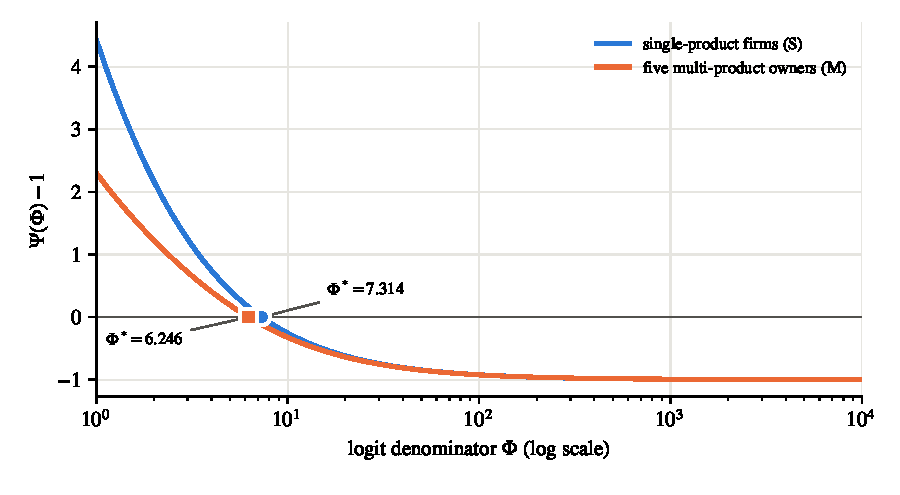
\includegraphics[width=0.82\linewidth]{figures/appC/psi.pdf}
\caption{The aggregate equation \eqref{eq:C-Psi}. Each curve plots $\Psi(\Phi) - 1$, where
$\Psi(\Phi) = \sum_fS_f(\Phi) + \frac{1}{\Phi}$ and $S_f(\Phi)$ solves $S_fe^{\frac{1}{1 - S_f}} = \frac{E_f}{\Phi}$. The curves
are strictly decreasing and cross zero once, at $\Phi^* = \frac{1}{s_0}$. At $\Phi = 1$ they equal 4.44 (S) and
2.31 (M). Computed with \texttt{figures/appC/src/logit\_bertrand.py}.}
\label{fig:C-psi}
\end{figure}

\casehead{Part (g)}
After the merger, owners 3 and 4 form one firm with 13 products, and the other owners are unchanged. Only $\Omega$
changes. \Cref{ex:04-merger-sim} introduces this merger and computes the cost reductions that would offset it. Here we
compare the equilibrium effects with first-round pricing pressure. By \cref{prop:C-unique} the post-merger equilibrium is unique, so the starting point of the iteration does
not matter. Best-response iteration converges in 16 iterations, and the column G of \cref{tab:C-logit-eq} reports the
result.

By \cref{prop:C-common-markup}, the merged firm charges one markup on all 13 products,
$m_M = \frac{1}{\alpha(1 - S_M)} = 0.821$, where $S_M = 39.12$ percent is its post-merger combined share. Before the
merger the markups were 0.636 (owner 3) and 0.670 (owner 4). Every product of owner 3 therefore rises in price by
0.185, and every product of owner 4 by 0.151. The mean increase over the 13 products is 0.167. Rivals respond with
smaller increases: 0.018 for owner 0, 0.013 for owner 2 and 0.004 for owner 1. \Cref{fig:C-logit-merger} plots the
change for every product. Firm-level shares, markups and profits before and after the merger are in
\cref{tab:04-merger-sim}.

The merged firm loses share, from 46.76 to 39.12 percent, and every rival gains. The outside share rises from 16.01
to 18.69 percent, and consumer surplus falls by 0.0773, from 0.9159 to 0.8387. Total profit rises from 0.5261 to
0.5767. The merger is profitable for its parties, whose joint profit rises by 5.0 percent, from 0.3061 to 0.3213.
The rivals gain more in percentage terms: 15.9 percent for owner 0, 16.7 percent for owner 1 and 16.3 percent for
owner 2. Total surplus falls from 1.4421 to 1.4154.

The fall in consumer surplus is an instance of a general result for multi-product logit pricing. A single number
summarizes each firm, its \emph{type}, which is its contribution to consumer surplus if it priced at marginal cost. In
our notation the type of firm $f$ is $E_f$. A merger without cost savings gives the merged firm the type $E_3 + E_4$,
the sum of the partners' types. \citet[Section~3.3.1, p.~229]{AskerNocke2021} report the following result of
\citet{NockeSchutz2019}. Consumer surplus does not fall if and only if the merged type is above a cutoff, which exceeds
the sum of the partners' types. A merger that only combines ownership, like this one, therefore always harms consumers. The aggregative structure behind the result is that of \cref{prop:C-unique}
\citep{NockeSchutz2018}.

\begin{figure}[htbp]
\centering
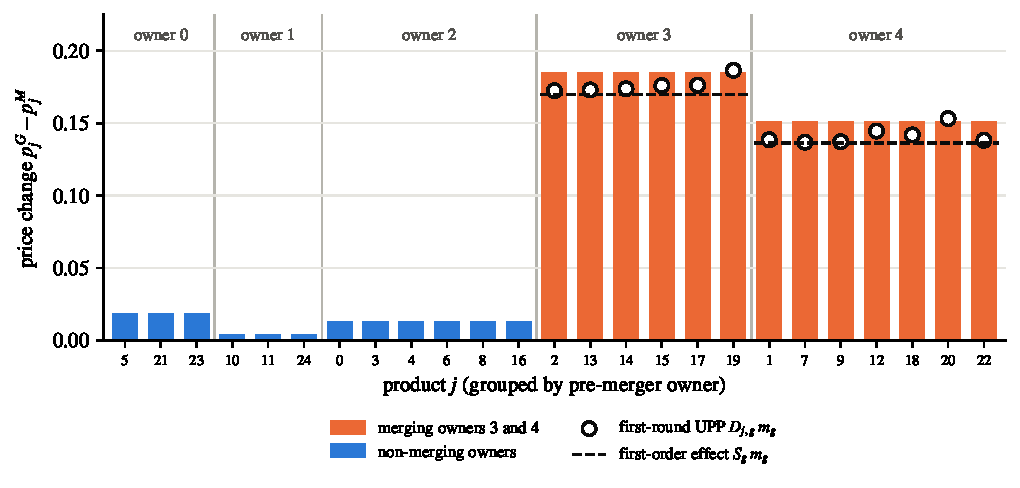
\includegraphics[width=\linewidth]{figures/appC/logit_merger.pdf}
\caption{Price changes caused by the merger of owners 3 and 4, by product. Bars show the change from the
pre-merger equilibrium (M) to the post-merger equilibrium (G). Hollow circles show each merging product's
first-round upward pricing pressure $D_{j,g}m_g$, and dashed lines show the first-order effect $S_gm_g$ of the
firm-level tax. Computed with \texttt{figures/appC/src/logit\_bertrand.py}.}
\label{fig:C-logit-merger}
\end{figure}

\emph{Upward pricing pressure} (UPP) measures the merger's incentive to raise prices at pre-merger prices
(\cref{sec:11-uppfs}). \citet{FarrellShapiro2010} define the first-round tax on product 1 of a merger between two
single-product firms as $t_1 = D_{12}(P_2 - C_2)$, the diversion ratio times the partner's margin (working-paper
version, p.~9). When the partner owns several products, the tax sums over them, $t_j = \sum_kD_{jk}m_k$
(\cref{eq:11-upp-multi}). For product $j$ of owner 3, the partner is owner 4, whose seven products share the
pre-merger markup $m_4$. With logit diversion,
\begin{equation}\label{eq:C-upp-logit}
  \mathit{UPP}_j = \sum_{k \in \mathcal{J}_4}\frac{s_k}{1 - s_j}\,m_4 = \frac{S_4}{1 - s_j}\,m_4 .
\end{equation}
The \emph{gross upward pricing pressure index} (GUPPI) divides by the product's price, $\mathit{GUPPI}_j = \frac{\mathit{UPP}_j}{p_j}$
(\cref{eq:11-guppi}). For owner 3's products, UPP ranges from 0.172 to 0.187 and GUPPI from 0.116 to 0.162. For
owner 4's products, UPP ranges from 0.137 to 0.153 and GUPPI from 0.078 to 0.132
(\cref{tab:C-logit-merger}). The UPP values bracket the equilibrium increases of 0.185 and 0.151 closely.
\citet[Section~3.3.2, pp.~230--231]{AskerNocke2021} present UPP as the simple alternative to full merger simulation.
Simulation estimates demand, recovers marginal costs from an assumption on conduct and solves for the post-merger
equilibrium. Demand and costs are known here, so this part carries out the last step exactly.

\begin{table}[htbp]
\centering
\caption{Pricing pressure and price changes of the merging products}
\label{tab:C-logit-merger}
\footnotesize
\begin{tabular}{@{}lcc@{}}
\toprule
 & Owner 3 (partner $g = 4$) & Owner 4 (partner $g = 3$) \\
\midrule
Product diversion to partner $\frac{S_g}{1 - s_j}$ & 0.257 to 0.278 & 0.215 to 0.241 \\
Product-level UPP $\frac{S_g}{1 - s_j}m_g$ & 0.172 to 0.187 & 0.137 to 0.153 \\
GUPPI $\frac{1}{p_j}\frac{S_g}{1 - s_j}m_g$ & 0.116 to 0.162 & 0.078 to 0.132 \\
Firm-level tax $t_f = \frac{S_gm_g}{1 - S_f}$ & 0.216 & 0.182 \\
First-order effect $(1 - S_f)t_f = S_gm_g$ & 0.170 & 0.136 \\
One round with taxes $t_f$, re-equilibrated & 0.184 & 0.152 \\
Equilibrium price change $m_M - m_f$ & 0.185 & 0.151 \\
\bottomrule
\end{tabular}

\vspace{3pt}
\begin{minipage}{0.97\textwidth}
\footnotesize Notes: Shares and markups are those of the pre-merger equilibrium M, $f$ is the merging owner and $g$
its partner. Ranges are across the owner's products. Firm-level shares, markups and profits before and after the
merger are in \cref{tab:04-merger-sim}. Computed with \texttt{figures/appC/src/logit\_bertrand.py}.
\end{minipage}
\end{table}

Three facts explain why the first-round measure predicts so well here. First, a multi-product firm's internal tax is
a firm-level object. Compare the merged firm's first-order condition for $j \in \mathcal{J}_3$ with owner 3's condition
when each of its products bears a cost increase $t_j$. By \eqref{eq:C-mp-foc} they coincide when
\begin{equation*}
  t_j - \sum_{k \in \mathcal{J}_3}s_kt_k = \sum_{k \in \mathcal{J}_4}s_km_k \qquad \text{for all } j \in \mathcal{J}_3 .
\end{equation*}
With a uniform tax and owner 4's common markup, the solution is $t_3 = \frac{S_4m_4}{1 - S_3}$. In general,
$t_f = \frac{S_gm_g}{1 - S_f}$ for merging firm $f$ with partner $g$. This exceeds the product-level UPP
\eqref{eq:C-upp-logit}, because a joint price increase on all of $f$'s products diverts a larger fraction of sales to
the partner. The firm-level taxes are 0.216 for owner 3 and 0.182 for owner 4.

Second, part (h) shows that a firm passes through a fraction $1 - S_f$ of a uniform cost increase when rivals'
prices are fixed. The first-order price effect is therefore $(1 - S_f)t_f = S_gm_g$, which equals 0.170 for owner 3
and 0.136 for owner 4. Rivals' responses add the rest. Imposing the taxes $t_f$ on owners 3 and 4 and letting all
five owners re-equilibrate gives increases of 0.184 and 0.152, within 0.001 of the merger. Recomputing the taxes at
the new prices and repeating, as Farrell and Shapiro propose, converges to the post-merger equilibrium in nine rounds.
The taxes barely move (owner 3's rises from 0.216 to 0.217), because logit diversion changes little.

Third, an exact decomposition shows the size of the remaining gap. Subtract owner $f$'s pre-merger condition
$m_f = \frac{1}{\alpha} + S_fm_f$ from the merged firm's condition $m_M = \frac{1}{\alpha} + (S_f' + S_g')m_M$, where
primes denote post-merger shares of the former product sets:
\begin{equation}\label{eq:C-merger-decomp}
  m_M - m_f = S_g'\,m_M + \big(S_f'\,m_M - S_f\,m_f\big) .
\end{equation}
For owner 3 the two terms are 0.180 and 0.006, and for owner 4 they are 0.142 and 0.010. The first term exceeds
$S_gm_g$ because the merged markup rises by more (23 and 29 percent) than the partner's share falls (14 and 19
percent). Product-level UPP exceeds $S_gm_g$ by the factor $\frac{1}{1 - s_j}$, between 1.005 and 1.125. The equilibrium
change exceeds $S_gm_g$ by 9 and 11 percent. The closeness of product-level UPP to the equilibrium change thus
reflects two separate corrections of similar size. Imposing the product-level UPP values as taxes, product by
product, would understate the firm's internal tax. Re-equilibrating with them gives increases of only 0.149 and
0.117.

\casehead{Part (h)}
Let all marginal costs rise by a unit tax $t$, so $mc_k(t) = mc_k + t$. Then $v_k(t) = v_k - \alpha t$ and
$E_f(t) = E_fe^{-\alpha t}$ for every firm.

\begin{proposition}[Logit pass-through]\label{prop:C-logit-passthrough}
Let demand be logit with constant marginal costs.
\begin{enumerate}[label=(\roman*)]
  \item Holding rivals' prices fixed, a uniform increase $dc$ in the marginal costs of firm $f$'s products raises
  each of its prices by $(1 - S_f)\,dc$. With one product, the pass-through is $1 - s_j$.
  \item In equilibrium, a common unit tax on all products has pass-through, at $t = 0$,
  \begin{equation}\label{eq:C-tax-pt}
    \rho_f = \frac{dp_k}{dt} = 1 - \frac{S_f\,s_0}{\big[(1 - S_f)^2 + S_f\big]\,(s_0 + \bar w)} \quad (k \in \mathcal{J}_f) ,
    \qquad \bar w = \sum_g\frac{S_g(1 - S_g)^2}{(1 - S_g)^2 + S_g} .
  \end{equation}
  With two or more firms, $1 - S_f < \rho_f < 1$.
\end{enumerate}
\end{proposition}

\begin{proof}
(i) This is \cref{prop:04-passthrough}(iii), and part (i) of that proposition is the single-product case.

(ii) The equilibrium satisfies \eqref{eq:C-h} for every firm and the adding-up condition \eqref{eq:C-Psi}. Since
$\ln h(S) = \ln S + \frac{1}{1 - S}$, differentiating \eqref{eq:C-h} in logarithms gives
\begin{equation*}
  \Big[\frac{1}{S_f} + \frac{1}{(1 - S_f)^2}\Big]dS_f = d\ln E_f - d\ln\Phi = -\alpha\,dt - d\ln\Phi .
\end{equation*}
Write $w_f = \frac{S_f(1 - S_f)^2}{(1 - S_f)^2 + S_f}$, the inverse of the bracket, so that
$dS_f = w_f(-\alpha\,dt - d\ln\Phi)$. Adding up gives $\sum_fdS_f = -d\frac{1}{\Phi} = s_0\,d\ln\Phi$. Summing the
previous equation over firms,
\begin{equation*}
  \bar w\,(-\alpha\,dt - d\ln\Phi) = s_0\,d\ln\Phi
  \quad\Longrightarrow\quad
  d\ln\Phi = -\frac{\alpha\bar w}{s_0 + \bar w}\,dt .
\end{equation*}
Substituting back, $-\alpha\,dt - d\ln\Phi = -\frac{\alpha s_0}{s_0 + \bar w}\,dt$, so
$dS_f = -\frac{\alpha w_fs_0}{s_0 + \bar w}\,dt$. Differentiating \eqref{eq:C-common-markup} then gives
\begin{equation*}
  dm_f = \frac{dS_f}{\alpha(1 - S_f)^2} = -\frac{S_f\,s_0}{\big[(1 - S_f)^2 + S_f\big](s_0 + \bar w)}\,dt ,
\end{equation*}
and $dp_k = dt + dm_f$ gives \eqref{eq:C-tax-pt}. Since $s_0 > 0$, $\rho_f < 1$. For the lower bound, write
$A_f = (1 - S_f)^2 + S_f$, so that $1 - A_f = S_f(1 - S_f)$. Then $\rho_f > 1 - S_f$ holds if and only if
$s_0 < A_f(s_0 + \bar w)$, that is, if and only if $S_f(1 - S_f)\,s_0 < A_f\bar w$. Since $\bar w \ge w_f$, the right
side is at least $A_fw_f = S_f(1 - S_f)^2$. This exceeds $S_f(1 - S_f)s_0$ because $1 - S_f > s_0$ when another firm
has a positive share.
\end{proof}

For a single product, part (i) is also the logit case of \cref{lem:11-passthrough}. Part (ii) gives in closed form, for any ownership structure, the common-tax pass-through
that \cref{cor:04-passthrough-eq} expresses through a matrix inverse for single-product firms. Two special cases help
to read it. Without an outside good ($s_0 \to 0$), a common cost increase is
passed through fully, because relative prices are all that matter. With a single firm, $\bar w = w_f$ and
$s_0 = 1 - S_f$, and \eqref{eq:C-tax-pt} reduces to $\rho_f = 1 - S_f$, the partial pass-through, because no rival
responds. With several firms, the common tax lowers every $E_f$, which by itself cuts $f$'s markup as in part (i). It
also raises rivals' prices, which lowers $\Phi_{-f}$ and offsets part of the fall in $z_f = \frac{E_fe^{-1}}{\Phi_{-f}}$.
Equilibrium pass-through therefore lies between the partial rate and one.

We compute the equilibrium at $t = 0.1$ by best-response iteration and divide each price change by $t$.
\Cref{tab:C-logit-tax} reports the results. Under S, product pass-through ranges from 0.980 to 0.999, with mean
0.994. It is lower for products with larger shares, and its correlation with the share is $-1.000$. Under M it ranges from 0.934 (owner 4) to 0.990 (owner 1),
with mean 0.954. The closed form \eqref{eq:C-tax-pt} at $t = 0$ gives almost the same values, and it matches a
numerical derivative to within $5\times10^{-8}$. Partial pass-through $1 - S_f$ is much lower, down to 0.746 for
owner 4. Rivals' responses account for most of the difference.

\begin{table}[htbp]
\centering
\caption{Pass-through of a common unit tax $t = 0.1$}
\label{tab:C-logit-tax}
\footnotesize
\begin{tabular}{@{}lcc@{}}
\toprule
 & Single-product firms (S) & Multi-product owners (M) \\
\midrule
\multicolumn{3}{@{}l}{\textit{Panel A. Market summary}} \\
Product pass-through at $t = 0.1$: range (mean) & 0.980 to 0.999 (0.994) & 0.934 to 0.990 (0.954) \\
Closed form \eqref{eq:C-tax-pt} at $t = 0$: range & 0.981 to 0.999 & 0.937 to 0.990 \\
Partial pass-through $1 - S_f$: range & 0.883 to 0.996 & 0.746 to 0.953 \\
Pass-through of the share-weighted mean price & 0.9895 & 0.9492 \\
\quad with weights held at pre-tax shares & 0.9893 & 0.9497 \\
\quad composition term & 0.0002 & $-0.0005$ \\
Outside share, before and after & 0.1367, 0.1618 & 0.1601, 0.1873 \\
Consumer surplus, before and after & 0.9949, 0.9107 & 0.9159, 0.8374 \\
Total profit, before and after & 0.4616, 0.4474 & 0.5261, 0.5051 \\
\bottomrule
\end{tabular}

\vspace{6pt}
\begin{tabular}{@{}lccccc@{}}
\toprule
\multicolumn{6}{@{}l}{\textit{Panel B. Owners under M}} \\
Owner & 0 & 1 & 2 & 3 & 4 \\
\midrule
Combined share $S_f$ (\%) & 18.87 & 4.67 & 13.68 & 21.40 & 25.36 \\
Partial pass-through $1 - S_f$ & 0.811 & 0.953 & 0.863 & 0.786 & 0.746 \\
Equilibrium pass-through, closed form at $t = 0$ & 0.955 & 0.990 & 0.969 & 0.949 & 0.937 \\
Equilibrium pass-through at $t = 0.1$ & 0.953 & 0.990 & 0.967 & 0.946 & 0.934 \\
\bottomrule
\end{tabular}

\vspace{3pt}
\begin{minipage}{0.97\textwidth}
\footnotesize Notes: Pass-through at $t = 0.1$ is $\frac{p(0.1) - p(0)}{0.1}$. The composition term is the difference
between the pass-through of the share-weighted mean price and the same object with weights fixed at pre-tax shares.
Computed with \texttt{figures/appC/src/logit\_bertrand.py}.
\end{minipage}
\end{table}

The share-weighted mean price $\bar p = \sum_jw_jp_j$, with $w_j = \frac{s_j}{1 - s_0}$, changes by
\begin{equation*}
  \frac{d\bar p}{dt} = \sum_jw_j\frac{dp_j}{dt} + \sum_jp_j\frac{dw_j}{dt} .
\end{equation*}
The first term is the average product pass-through. The second is a composition term, which is positive when
consumers shift toward expensive products. The mean-price pass-through is 0.9895 under S and 0.9492 under M, and the
composition terms are only 0.0002 and $-0.0005$. A common unit tax shifts all logit prices by similar amounts, so
substitution among inside goods hardly changes the mix.

These results bear on the cigarette tax study of \cref{sec:C-passthrough}. With logit demand and constant marginal
costs, a common tax is passed through less than one for one by every firm, whatever the ownership structure, and
composition effects are negligible. Logit demand is log-concave in own price, which is why pass-through stays below
one. A pass-through rate above one, as \citet{Sumner1981} estimates, needs a feature that this model lacks. Candidates
are demand that is more convex than the logit, composition effects much larger than those found here, or a different
form of conduct.

\subsection{Computational notes}

A single script produces every number in this section. It is \texttt{logit\_bertrand.py} in the folder
\texttt{figures/appC/src}, and it reads the data file \texttt{logit\_market.csv} from the folder
\texttt{figures/appC/data}.
\begin{enumerate}
  \item Compute $a_j = x_j\beta + \xi_j$, $mc_j$ and $v_j = a_j - \alpha\,mc_j$. An owner vector assigns products to
  firms. Under S it is $(0, 1, \dots, 24)$. After the merger, owner 4 is relabeled 3.
  \item For each firm compute $E_f = \sum_{k \in \mathcal{J}_f}e^{v_k}$ once. At each iteration compute
  $\Phi_{-f} = \Phi - \sum_{k \in \mathcal{J}_f}e^{\delta_k}$, the markup \eqref{eq:C-br-multi} with the principal
  branch of $W$, and the new prices.
  \item Stop when the sup-norm change in prices is below $10^{-12}$. Verify \eqref{eq:C-stacked-foc}, the common
  markups \eqref{eq:C-common-markup} and agreement with markup iteration and a root finder.
  \item For uniqueness, solve \eqref{eq:C-h} for $S_f(\Phi)$ in logarithms, $\ln S_f + \frac{1}{1 - S_f} = \ln\frac{E_f}{\Phi}$,
  with a bracketing root finder, and evaluate $\Psi$ on the grid.
  \item For the merger and the tax, re-solve with the new owner vector or with $mc + t$.
\end{enumerate}
The best-response step takes five lines in Python with NumPy and SciPy:
\begin{verbatim}
def best_response(p, owner, mc):
    e = np.exp(a - alpha * p)                                # e^{delta_j}
    E = np.bincount(owner, weights=np.exp(a - alpha * mc))   # E_f
    phi_minus = 1 + e.sum() - np.bincount(owner, weights=e)  # Phi_{-f}
    m = (1 + lambertw(E * np.exp(-1) / phi_minus).real) / alpha
    return mc + m[owner]
\end{verbatim}

\section{Simulating a market with random coefficients demand}\label{sec:C-simulate}

The previous problem computed prices from a known demand system. Empirical work runs in the opposite direction,
from observed prices and shares back to demand and cost. To judge an estimator we need data whose true model we
know. This problem builds such data, and the next three problems use it. We simulate 100 markets
from a random coefficients logit model with multi-product Bertrand pricing, solve for equilibrium prices, and draw the
choices of about ten thousand consumers per market. Sections \ref{sec:C-vertical} to \ref{sec:C-rc-est} estimate the
vertical, logit and random coefficients models on the resulting data. \Cref{sec:08-worked} uses the same design to
illustrate the estimation of the random coefficients model step by step.

\subsection{Statement}

Think of the market for yogurt in 100 metropolitan areas, which we treat as independent markets $t = 0, \dots, 99$.
Ten products exist in total, $j = 1, \dots, 10$. Each market offers between 4 and 9 of them, 6.54 on average, so there
are 654 product-market observations. A product has three characteristics,
$x_{jt} = (1, x^{sug}_{jt}, x^{org}_{jt})$: a constant, its sugar content and an indicator of organic production. Its
marginal cost also depends on a cost shifter $w_{jt}$, the price of milk used in production. Characteristics, the
cost shifter and the owner are fixed by product, so $x_{jt} = x_j$ and $w_{jt} = w_j$ in every market that offers
$j$ (\cref{tab:C-products}). Four firms own the products: firm A owns $\{5, 8\}$, firm B owns $\{1, 4, 6, 7\}$, firm C
owns $\{2, 3, 10\}$ and firm D owns $\{9\}$. Across markets only the set of products offered $\mathcal{J}_t$, the
unobservables $(\xi_{jt}, \omega_{jt})$ and the market size $M_t$ vary. Their values are supplied in the file
\texttt{yogurt\_markets.csv} in the folder \texttt{figures/appC/data}. Market sizes range from 9,756 to 10,223, with
mean 9,998.7.

Consumer $i$ in market $t$ has utility
\begin{equation}\label{eq:C-rc-utility}
  u_{ijt} = \delta_{jt} + \tilde x_{jt}\Sigma\nu_i + \epsilon_{ijt} , \qquad
  \delta_{jt} = x_{jt}\beta - \alpha p_{jt} + \xi_{jt} , \qquad
  u_{i0t} = \epsilon_{i0t} ,
\end{equation}
where $\tilde x_{jt} = (x_{jt}, p_{jt})$ contains the characteristics and the price, $\nu_i \sim N(0, I_4)$, and the
$\epsilon_{ijt}$ are independent type-I extreme value shocks. The parameters are $\beta = (-1, 0.2, 0.15)$,
$\alpha = 3$ and $\Sigma = \diag(\Sigma_{11}, \Sigma_{22}, \Sigma_{33}, \Sigma_{pp}) = \diag(0.5, 0.2, 0.3, 0.5)$.
Marginal cost is
\begin{equation}\label{eq:C-rc-mc}
  mc_{jt} = x_{jt}\gamma_1 + \gamma_2w_{jt} + \omega_{jt} , \qquad \gamma_1 = (0.2, 0.25, 0.3) , \quad \gamma_2 = 0.5 .
\end{equation}
The demand and cost shocks are drawn independently of each other and of the characteristics. Their sample standard
deviations are 0.50 for $\xi_{jt}$ and 0.050 for $\omega_{jt}$, and their sample correlation is 0.004. Firms know all
characteristics, shocks and parameters. Each firm evaluates expected demand by averaging over $n_s = 100$ consumer
types drawn once for each market.

\begin{table}[htbp]
\centering
\caption{Products in the simulated markets}
\label{tab:C-products}
\footnotesize
\begin{tabular}{@{}lcccccccccc@{}}
\toprule
Product $j$ & 1 & 2 & 3 & 4 & 5 & 6 & 7 & 8 & 9 & 10 \\
\midrule
Firm & B & C & C & B & A & B & B & A & D & C \\
Sugar content $x^{sug}_j$ & 1.349 & 1.300 & 0.929 & 1.315 & 1.182 & 0.636 & 1.130 & 1.204 & 1.128 & 0.879 \\
Organic $x^{org}_j$ & 0 & 1 & 0 & 1 & 0 & 0 & 0 & 0 & 1 & 0 \\
Price of milk $w_j$ & 0.534 & 0.367 & 0.426 & 0.547 & 0.346 & 0.529 & 0.588 & 0.334 & 0.527 & 0.442 \\
\midrule
Markets offering $j$ & 77 & 58 & 73 & 65 & 52 & 66 & 66 & 68 & 65 & 64 \\
Mean price & 1.189 & 1.403 & 1.025 & 1.504 & 1.048 & 1.008 & 1.164 & 1.039 & 1.427 & 1.012 \\
Mean markup & 0.390 & 0.395 & 0.381 & 0.402 & 0.378 & 0.384 & 0.390 & 0.376 & 0.378 & 0.382 \\
Mean realized share & 0.015 & 0.010 & 0.024 & 0.009 & 0.023 & 0.024 & 0.019 & 0.027 & 0.011 & 0.024 \\
\bottomrule
\end{tabular}

\vspace{3pt}
\begin{minipage}{0.97\textwidth}
\footnotesize Notes: The first four rows are the design. The last three rows are equilibrium outcomes, averaged over
the markets that offer the product. In the data file the owner codes of firms A, B, C and D are 0, 1, 2 and 4.
Computed with \texttt{figures/appC/src/appC\_simulate.py}.
\end{minipage}
\end{table}

\begin{enumerate}[label=(\alph*)]
  \item Interpret the random coefficients. How likely is a consumer to like higher prices?
  \item Write the expected-share function that the firms use, with $n_s = 100$ fixed draws per market, and explain how
  to evaluate it without numerical overflow.
  \item Derive the first-order conditions of multi-product Bertrand pricing and an algorithm that solves them. Solve
  every market and check the solutions.
  \item Simulate the realized shares of $M_t$ consumers per market and compare them with the expected shares.
  \item Report the equilibrium of market 0.
  \item Show that, when individual choice probabilities are small, the markup of product $j$ is close to the inverse
  of the average price sensitivity of its buyers. Evaluate the approximation in market 0.
  \item Derive the sampling error of a realized share and of its logarithm, and evaluate it in market 0.
\end{enumerate}

\subsection{Solution}

\casehead{Part (a)}
Because $\Sigma$ is diagonal, the consumer-specific term in \eqref{eq:C-rc-utility} is
\begin{equation*}
  \tilde x_{jt}\Sigma\nu_i = 0.5\,\nu_{i1} + 0.2\,\nu_{i2}x^{sug}_{jt} + 0.3\,\nu_{i3}x^{org}_{jt} + 0.5\,\nu_{i4}p_{jt} .
\end{equation*}
Consumer $i$ therefore has her own coefficients
\begin{equation}\label{eq:C-rc-coefs}
  \beta_{i1} = -1 + 0.5\,\nu_{i1} , \quad \beta_{i2} = 0.2 + 0.2\,\nu_{i2} , \quad
  \beta_{i3} = 0.15 + 0.3\,\nu_{i3} , \quad -\alpha_i \text{ with } \alpha_i = 3 - 0.5\,\nu_{i4} .
\end{equation}
The random constant $\beta_{i1}$ shifts the utility of every inside good relative to the outside good. Consumers
who like yogurt are more likely to buy some yogurt. Inside goods therefore substitute more with one another than
with the outside good, as in a nested logit with one nest of inside goods. The coefficients on sugar and on organic
production are positive on average, but 15.9 percent of consumers dislike sugar ($\nu_{i2} < -1$) and 30.9 percent
dislike organic production ($\nu_{i3} < -0.5$). The price sensitivity $\alpha_i$ is normal with mean 3 and standard
deviation 0.5. A consumer likes higher prices only if $\alpha_i \le 0$, that is, if $\nu_{i4} \ge 6$. This has
probability $\Pr(\nu_{i4} \ge 6) = 9.9\times10^{-10}$. Among the 10,000 consumer types the firms use, $\alpha_i$
ranges from 1.17 to 4.79.

Conditional on $\nu_i$, the extreme value shocks give logit choice probabilities. With
$V_{ijt} = \delta_{jt} + \tilde x_{jt}\Sigma\nu_i$,
\begin{equation}\label{eq:C-rc-sij}
  s_{ijt} = \frac{e^{V_{ijt}}}{1 + \sum_{k \in \mathcal{J}_t}e^{V_{ikt}}} , \qquad
  s_{jt} = \int_{\R^4} s_{ijt}(\nu)\,\phi_4(\nu)\,\dd\nu ,
\end{equation}
where $s_{ijt}(\nu)$ is the choice probability of a consumer with taste vector $\nu$ and $\phi_4$ is the
four-dimensional standard normal density. The integral breaks the
independence of irrelevant alternatives. A rise in $p_{kt}$ moves consumers who were likely to buy $k$, and these
consumers are most likely to buy products similar to $k$ (\cref{prop:08-derivs}). Cross elasticities therefore vary
across products, unlike \eqref{eq:C-logit-elast}.

\casehead{Part (b)}
For each market we draw $n_s = 100$ vectors $\nu_{it} \sim N(0, I_4)$ once and keep them fixed. They are the consumer
types whose average demand the firms compute. The expected share of product $j$ is the simulator of
\citet[eq.~11, p.~532]{Nevo2000a},
\begin{equation}\label{eq:C-rc-simshare}
  s_{jt}(p_t) = \frac{1}{n_s}\sum_{i=1}^{n_s}s_{ijt}(p_t) , \qquad
  s_{ijt}(p_t) = \frac{e^{V_{ijt}}}{1 + \sum_{k \in \mathcal{J}_t}e^{V_{ikt}}} .
\end{equation}
Prices enter twice, through $\delta_{jt}$ and through the last element of $\tilde x_{jt}$, so the function must rebuild
$\tilde x_{jt}$ whenever prices change.

Exponentials overflow when utilities are large. For draw $i$, let $c_i = \max\{0, \max_kV_{ikt}\}$, where the 0 is the
outside good's utility. Multiplying the numerator and the denominator of $s_{ijt}$ by $e^{-c_i}$ gives
\begin{equation*}
  s_{ijt} = \frac{e^{V_{ijt} - c_i}}{e^{-c_i} + \sum_{k \in \mathcal{J}_t}e^{V_{ikt} - c_i}} .
\end{equation*}
The value is unchanged. Every exponent is now at most zero, so nothing overflows, and the largest term in the
denominator equals one, so the denominator cannot underflow to zero.

The draws stay fixed for two reasons. With fixed draws, $s_t(p_t)$ is a smooth deterministic function of prices, so the
first-order conditions of part (c) define a well-posed system. With fresh draws at each evaluation, the system would
change from one iteration to the next, and no solver could converge. In this design the 100 draws also define what
firms believe about demand. Part (d) shows that these beliefs differ from population demand by simulation error.

\casehead{Part (c)}
Firm $f$ owns the products $\mathcal{J}_{ft} \subseteq \mathcal{J}_t$ and earns
$\pi_{ft} = M_t\sum_{k \in \mathcal{J}_{ft}}(p_{kt} - mc_{kt})s_{kt}(p_t)$. Market size multiplies profit, so it drops out of
the first-order conditions
\begin{equation}\label{eq:C-rc-foc}
  s_{jt} + \sum_{k \in \mathcal{J}_{ft}}(p_{kt} - mc_{kt})\frac{\partial s_{kt}}{\partial p_{jt}} = 0 , \qquad j \in \mathcal{J}_{ft} .
\end{equation}
These are equations (3.3) of \citet[p.~853]{BerryLevinsohnPakes1995}. For draw $i$, price enters $V_{ijt}$ with
coefficient $\frac{\partial V_{ijt}}{\partial p_{jt}} = -\alpha + 0.5\,\nu_{i4} = -\alpha_i$. The quotient rule of
\cref{sec:C-logit-bertrand}, applied draw by draw, gives
$\frac{\partial s_{ijt}}{\partial p_{kt}} = \alpha_is_{ijt}(s_{ikt} - \indic\{j = k\})$. Averaging over draws,
\begin{equation}\label{eq:C-rc-deriv}
  \Delta_{jk,t} = \frac{\partial s_{jt}}{\partial p_{kt}} = \frac{1}{n_s}\sum_{i=1}^{n_s}\alpha_is_{ijt}\big(s_{ikt} - \indic\{j = k\}\big) .
\end{equation}
With $\Omega_t$ the ownership matrix of market $t$, the conditions stack as in \eqref{eq:C-stacked-foc}:
$s_t + (\Omega_t \odot \Delta_t^\top)(p_t - mc_t) = 0$. Solving for the markups gives
$p_t - mc_t = -(\Omega_t \odot \Delta_t^\top)^{-1}s_t$, which is equation (3.5) of
\citet[p.~854]{BerryLevinsohnPakes1995} with their matrix equal to $-(\Omega_t \odot \Delta_t^\top)$.

\begin{proposition}[Morrow-Skerlos fixed point]\label{prop:C-ms}
Let $\Lambda_t$ be the diagonal matrix with $\Lambda_{jj,t} = \frac{1}{n_s}\sum_i\alpha_is_{ijt}$, and let $\Gamma_t$ be
the matrix with $\Gamma_{jk,t} = \frac{1}{n_s}\sum_i\alpha_is_{ijt}s_{ikt}$. If every $\alpha_i > 0$, the first-order
conditions hold at $p_t$ if and only if
\begin{equation}\label{eq:C-ms-zeta}
  p_t - mc_t = \zeta_t(p_t) \equiv \Lambda_t^{-1}\big[s_t + (\Omega_t \odot \Gamma_t)(p_t - mc_t)\big] ,
\end{equation}
where $\Lambda_t$, $\Gamma_t$ and $s_t$ are evaluated at $p_t$.
\end{proposition}

\begin{proof}
By \eqref{eq:C-rc-deriv}, $\Delta_t = -\Lambda_t + \Gamma_t$, and $\Gamma_t$ is symmetric. Since $\Omega_t$ is symmetric
with a unit diagonal, $\Omega_t \odot \Lambda_t = \Lambda_t$, and
\begin{equation*}
  (\Omega_t \odot \Delta_t)^\top = -\Lambda_t + \Omega_t \odot \Gamma_t .
\end{equation*}
The first-order conditions therefore read $s_t - \Lambda_t(p_t - mc_t) + (\Omega_t \odot \Gamma_t)(p_t - mc_t) = 0$.
Every diagonal entry of $\Lambda_t$ is positive because $\alpha_i > 0$ and $s_{ijt} > 0$. Moving the $\Lambda_t$ term
to the left and multiplying by $\Lambda_t^{-1}$ gives \eqref{eq:C-ms-zeta}. Each step is reversible.
\end{proof}

This is \cref{prop:08-ms}, due to \citet{MorrowSkerlos2011}. In the plain logit, $\alpha_i = \alpha$ gives
$\Lambda_{jj} = \alpha s_j$ and $\Gamma_{jk} = \alpha s_js_k$, and \eqref{eq:C-ms-zeta} becomes
$m_j = \frac{1}{\alpha} + \sum_{k \in \mathcal{J}_f}s_km_k$, the multi-product condition \eqref{eq:C-mp-foc}. Here every
$\alpha_i$ exceeds 1.17, so the proposition applies. We solve each market as follows.
\begin{enumerate}
  \item Start at $p_t^{(0)} = mc_t$.
  \item Given $p_t^{(n)}$, compute $s_{ijt}$ for the 100 draws, then $s_t$, $\Lambda_t$ and $\Gamma_t$.
  \item Set $p_t^{(n+1)} = mc_t + \zeta_t(p_t^{(n)})$.
  \item Stop when $\|p_t^{(n+1)} - p_t^{(n)}\|_\infty < 10^{-12}$. Otherwise return to step 2.
  \item Verify the first-order conditions \eqref{eq:C-rc-foc} at the solution.
\end{enumerate}
Nothing guarantees that $p \mapsto mc + \zeta(p)$ is a contraction, so convergence must be checked market by market.

\Cref{tab:C-sim-checks} reports the diagnostics. The iteration converges in every market, in 10 to 13 iterations
(11.05 on average). The largest first-order residual across markets is $8.6\times10^{-15}$. A hybrid Powell root finder
on \eqref{eq:C-rc-foc}, started at marginal cost, reaches the same prices to within $1.0\times10^{-13}$. We then restart
from 20 random price vectors per market, with each price drawn uniformly on $[0, 4]$. All 2,000 runs of the
iteration return the original prices, to within $2.1\times10^{-13}$, so no market shows a second equilibrium.

The root finder is less reliable from the random starts. Applied to the residual of \eqref{eq:C-rc-foc}, it solves
only 13 of the 2,000 problems. Every term of that residual tends to zero as prices rise without bound. The root
finder can therefore stop at very high prices, where the residual is small and no equilibrium is near. Applied to the residual
$\zeta_t(p) - (p - mc_t)$, which is measured in price units, it solves 1,817 of the 2,000 problems, and every
solution it finds is the original one.

Equilibrium prices range from 0.881 to 1.609, with mean 1.180. Markups range from 0.348 to 0.451, with mean 0.386,
and the Lerner index averages 0.334. Markups are close to the inverse of the mean price coefficient,
$\frac{1}{3} = 0.333$, for a reason that part (f) makes precise.

\begin{table}[htbp]
\centering
\caption{Simulated markets: equilibrium computation and realized shares}
\label{tab:C-sim-checks}
\footnotesize
\begin{tabular}{@{}lr@{}}
\toprule
\multicolumn{2}{@{}l}{\textit{Panel A. Equilibrium prices}} \\
Morrow-Skerlos iterations per market, range (mean) & 10 to 13 (11.05) \\
Largest first-order residual & $8.6\times10^{-15}$ \\
Largest price difference, iteration versus root finder & $1.0\times10^{-13}$ \\
Random restarts solved by the iteration, largest deviation & 2,000 of 2,000, $2.1\times10^{-13}$ \\
Random restarts solved by a root finder on \eqref{eq:C-rc-foc} & 13 of 2,000 \\
Random restarts solved by a root finder on $\zeta_t(p) - (p - mc_t)$ & 1,817 of 2,000 \\
Markets with a second equilibrium & 0 \\
Prices: range (mean) & 0.881 to 1.609 (1.180) \\
Markups: range (mean) & 0.348 to 0.451 (0.386) \\
Lerner index: range (mean) & 0.234 to 0.448 (0.334) \\
\midrule
\multicolumn{2}{@{}l}{\textit{Panel B. Realized shares}} \\
Simulated consumers & 999,870 \\
Products with zero realized share & 0 \\
Smallest realized share (buyers) & 0.0019 (19) \\
Mean and largest absolute gap, realized minus expected share & 0.0014, 0.0100 \\
Correlation of realized and expected shares & 0.986 \\
Outside share: mean (range across markets) & 0.879 (0.788 to 0.948) \\
Mean squared standardized gap: realized minus population share & 1.07 \\
Mean squared standardized gap: expected minus population share & 0.84 \\
Mean squared standardized gap: realized minus expected share & 1.88 \\
\bottomrule
\end{tabular}

\vspace{3pt}
\begin{minipage}{0.97\textwidth}
\footnotesize Notes: 654 product-market observations in 100 markets. Random restarts draw each starting price from
$U[0, 4]$, 20 per market. A run counts as solved when the largest markup residual is below $10^{-10}$. Standardized
gaps divide by the sampling standard deviation $\sqrt{\frac{s(1 - s)}{M_t}}$, where $s$ is the population share
computed with 100,000 draws. Computed with \texttt{figures/appC/src/appC\_simulate.py}.
\end{minipage}
\end{table}

\casehead{Part (d)}
At the equilibrium prices we simulate the choices of $M_t$ consumers in each market. Each consumer receives a fresh
draw $\nu_i \sim N(0, I_4)$ and $|\mathcal{J}_t| + 1$ fresh extreme value shocks, one for each product and one for the
outside good. She chooses the alternative with the highest utility $u_{ijt}$. The \emph{realized share} of product $j$
is the fraction of consumers who choose it,
\begin{equation}\label{eq:C-realized}
  \hat s_{jt} = \frac{q_{jt}}{M_t} , \qquad q_{jt} = \sum_{i=1}^{M_t}\indic\Big\{j = \argmax_{k \in \mathcal{J}_t \cup \{0\}}u_{ikt}\Big\} .
\end{equation}
Realized shares, prices, characteristics, the cost shifter and ownership are the data that Sections
\ref{sec:C-vertical} to \ref{sec:C-rc-est} use. The unobservables, the marginal costs and the expected shares are
kept only to evaluate the estimators.

In total we simulate 999,870 consumers. No product has a zero realized share, and the smallest realized share is
0.0019, or 19 buyers. The mean absolute difference between realized and expected shares is 0.0014, the largest is
0.0100, and their correlation is 0.986. The outside good is large. Its realized share averages 0.879 across markets
and ranges from 0.788 to 0.948.

Three share concepts are at work. The expected share $s_{jt}$ averages over the firms' 100 draws. The
\emph{population share} $s^\infty_{jt}$ integrates over the whole normal distribution, and we approximate it with
100,000 draws per market. The realized share $\hat s_{jt}$ is a sample proportion among $M_t$ consumers drawn from the
population. The gap between realized and expected shares therefore has two parts,
\begin{equation*}
  \hat s_{jt} - s_{jt} = \big(\hat s_{jt} - s^\infty_{jt}\big) + \big(s^\infty_{jt} - s_{jt}\big) ,
\end{equation*}
\emph{sampling error} from the finite number of consumers and \emph{simulation error} from the finite number of firm
draws. Part (g) shows that the sampling error has standard deviation close to $\sqrt{\frac{s(1 - s)}{M_t}}$. Dividing
each part by this standard deviation and averaging the squares over the 654 observations gives 1.07 for the sampling
part, close to the value of one that the binomial formula predicts. It gives 0.84 for the simulation part, and 1.88
for the total. With $n_s = 100$, the firms' simulation error is about as large as the sampling error of
ten thousand consumers. The median relative simulation error $|\frac{s_{jt}}{s^\infty_{jt}} - 1|$ is 4.7 percent, and
the largest is 29 percent.

\casehead{Part (e)}
\Cref{tab:C-mkt0} reports market 0, which offers products 2, 3, 4, 6, 8, 9 and 10 and has $M_0 = 9{,}880$ consumers.
Markups lie between 0.375 and 0.400. The Lerner index ranges from 0.260 for product 9, the most expensive product, to
0.408 for product 10, the cheapest. The outside good's expected share is 0.8463 and its realized share is 0.8549.
Realized and expected shares are close. The largest relative gaps are $-20$ percent for product 9 and $-11$ percent
for product 10. In market 0 the firms' 100 draws overstate demand for every inside product. The expected shares
exceed the population shares by 4 to 10 percent, and the population outside share is 0.8555.

\begin{table}[htbp]
\centering
\caption{Equilibrium in market 0 and the anatomy of its markups}
\label{tab:C-mkt0}
\footnotesize
\setlength{\tabcolsep}{4.5pt}
\begin{tabular}{@{}lcccccccccc@{}}
\toprule
 & & & & & \multicolumn{3}{c}{Share} & & & \\
\cmidrule(lr){6-8}
Product & Firm & $mc_j$ & $p_j$ & $m_j$ & Expected & Realized & Population & Buyers $q_j$ & $\frac{1}{\bar\alpha_j}$ & $\Gamma$ term \\
\midrule
2 & C & 0.9204 & 1.3200 & 0.3995 & 0.0048 & 0.0052 & 0.0044 & 51 & 0.3669 & 0.0326 \\
3 & C & 0.6308 & 1.0182 & 0.3874 & 0.0272 & 0.0252 & 0.0259 & 249 & 0.3584 & 0.0290 \\
4 & B & 1.0286 & 1.4196 & 0.3910 & 0.0125 & 0.0126 & 0.0113 & 124 & 0.3703 & 0.0207 \\
6 & B & 0.6238 & 0.9993 & 0.3755 & 0.0200 & 0.0203 & 0.0192 & 201 & 0.3583 & 0.0172 \\
8 & A & 0.7291 & 1.1246 & 0.3955 & 0.0593 & 0.0560 & 0.0556 & 553 & 0.3616 & 0.0339 \\
9 & D & 1.0729 & 1.4497 & 0.3768 & 0.0072 & 0.0058 & 0.0066 & 57 & 0.3717 & 0.0051 \\
10 & C & 0.5585 & 0.9429 & 0.3845 & 0.0226 & 0.0201 & 0.0215 & 199 & 0.3559 & 0.0285 \\
\midrule
Outside good & & & & & 0.8463 & 0.8549 & 0.8555 & 8,446 & & \\
\bottomrule
\end{tabular}

\vspace{3pt}
\begin{minipage}{0.97\textwidth}
\footnotesize Notes: $M_0 = 9{,}880$. Expected shares average over the firms' 100 draws, population shares over
100,000 draws, and realized shares are fractions of the $M_0$ simulated consumers. $\bar\alpha_j$ is the mean price
sensitivity of product $j$'s buyers among the firms' draws, and the $\Gamma$ term is the second term of
\eqref{eq:C-markup-decomp}, so $m_j = \frac{1}{\bar\alpha_j} + \Gamma$ term. Computed with
\texttt{figures/appC/src/appC\_simulate.py}.
\end{minipage}
\end{table}

\casehead{Part (f)}
Rewrite \eqref{eq:C-ms-zeta} product by product. Dividing the $j$-th row by $\Lambda_{jj}$ gives the exact decomposition
\begin{equation}\label{eq:C-markup-decomp}
  m_j = \frac{s_j}{\Lambda_{jj}} + \frac{1}{\Lambda_{jj}}\sum_{k \in \mathcal{J}_f}\Gamma_{jk}m_k .
\end{equation}

\begin{proposition}[Markups and the price sensitivity of buyers]\label{prop:C-buyer-alpha}
Suppose every $\alpha_i > 0$. Let $\bar\alpha_j = \frac{\Lambda_{jj}}{s_j}$.
\begin{enumerate}[label=(\roman*)]
  \item $\bar\alpha_j$ is the mean price sensitivity of product $j$'s buyers,
  \begin{equation}\label{eq:C-buyer-alpha}
    \bar\alpha_j = \frac{\sum_i\alpha_is_{ij}}{\sum_is_{ij}} = \E\big[\alpha_i \mid i \text{ buys } j\big] ,
  \end{equation}
  where the expectation is over the $n_s$ consumer types and their extreme value shocks.
  \item The markup satisfies
  \begin{equation}\label{eq:C-buyer-bound}
    \Big|m_j - \frac{1}{\bar\alpha_j}\Big| \le \Big(\max_{k \in \mathcal{J}_f}|m_k|\Big)\sum_{k \in \mathcal{J}_f}\max_is_{ik} .
  \end{equation}
  Hence $m_j$ approaches $\frac{1}{\bar\alpha_j}$ as the individual choice probabilities of firm $f$'s products tend to
  zero.
\end{enumerate}
\end{proposition}

\begin{proof}
(i) Each type is equally likely, with probability $\frac{1}{n_s}$, and type $i$ buys $j$ with probability $s_{ij}$. By
Bayes' rule, the probability that a buyer of $j$ is of type $i$ is $\frac{s_{ij}}{\sum_{i'}s_{i'j}}$. Averaging
$\alpha_i$ with these weights gives \eqref{eq:C-buyer-alpha}, and the factor $\frac{1}{n_s}$ cancels from
$\frac{\Lambda_{jj}}{s_j}$.

(ii) By \eqref{eq:C-markup-decomp}, $m_j - \frac{1}{\bar\alpha_j} = \sum_{k \in \mathcal{J}_f}\frac{\Gamma_{jk}}{\Lambda_{jj}}m_k$.
Each ratio is a weighted average of $s_{ik}$ over types, with non-negative weights $\alpha_is_{ij}$:
\begin{equation*}
  \frac{\Gamma_{jk}}{\Lambda_{jj}} = \frac{\sum_i\alpha_is_{ij}\,s_{ik}}{\sum_i\alpha_is_{ij}} \le \max_is_{ik} .
\end{equation*}
The triangle inequality gives \eqref{eq:C-buyer-bound}.
\end{proof}

The markup is thus the inverse of the buyers' mean price sensitivity, corrected by a term of the order of the
firm's individual choice probabilities. This is the discrete-choice form of the inverse semi-elasticity rule
(\cref{eq:08-ms-approx}). In the plain logit, $\bar\alpha_j = \alpha$ for every product, which is why all markups in
\cref{sec:C-logit-bertrand} lie near $\frac{1}{\alpha}$. With random coefficients, buyers select themselves. Consumers
with high $\alpha_i$ buy the outside good more often, so the buyers of any inside product are less price sensitive
than the population.

\Cref{tab:C-mkt0} evaluates the decomposition in market 0. The mean of $\alpha_i$ over the firms' 100 draws is 3.028,
and the mean among consumers who choose the outside good is 3.075. The buyers' mean sensitivity $\bar\alpha_j$ ranges
from 2.690 (product 9) to 2.810 (product 10). Its inverse lies between 0.356 and 0.372 and accounts for 91 to 99
percent of each markup. The expensive organic products 9 and 4 attract the least price-sensitive buyers, with
$\bar\alpha_j$ of 2.690 and 2.701. The $\Gamma$ term accounts for the rest, between 1.4 and 8.6 percent of the markup.
It has two parts. The diagonal part restores the factor $1 - s_{ij}$ in each type's own-price derivative and is
largest for product 8 (0.034), the product with the largest share. The off-diagonal part is the value of sales
recaptured by the firm's other products and is largest for firm C's product 2 (0.029). Firm D sells one product, so
product 9 has no recapture. Product 2 carries the highest markup in the market, 0.3995, although its buyers are more
price sensitive than those of products 4 and 9. Firm C's recapture of 0.029 lifts it to the top. Net of the recapture
terms, product 2's markup is 0.370, the fifth highest of the seven.

\casehead{Part (g)}
Given prices, the $M_t$ consumers choose independently, and each chooses $j$ with probability $s^\infty_{jt}$. Hence
$q_{jt}$ is binomial with parameters $M_t$ and $s^\infty_{jt}$. Writing $s$ for $s^\infty_{jt}$,
\begin{equation}\label{eq:C-share-var}
  \E[\hat s_{jt}] = s , \qquad \Var(\hat s_{jt}) = \frac{s(1 - s)}{M_t} .
\end{equation}
The inversions in Sections \ref{sec:C-vertical} to \ref{sec:C-rc-est} use logarithms of shares. A first-order Taylor
expansion, $\ln\hat s_{jt} \approx \ln s + \frac{\hat s_{jt} - s}{s}$, gives the delta-method variance
(\cref{app:econometrics}),
\begin{equation}\label{eq:C-logshare-var}
  \Var(\ln\hat s_{jt}) \approx \frac{1 - s}{M_ts} = \frac{1 - s}{\E[q_{jt}]} .
\end{equation}
The standard error of a log share is about one over the square root of the number of buyers. A second-order expansion
gives the bias $\E[\ln\hat s_{jt}] - \ln s \approx -\frac{\Var(\hat s_{jt})}{2s^2} = -\frac{1 - s}{2M_ts}$, the
sampling analogue of the simulation bias in \cref{prop:08-simbias}. The logit inversion of \cref{ch:logit} uses the
difference $\ln\hat s_{jt} - \ln\hat s_{0t}$. Since $\Cov(\hat s_{jt}, \hat s_{0t}) = -\frac{s_{jt}s_{0t}}{M_t}$, the
delta method gives $\Cov(\ln\hat s_{jt}, \ln\hat s_{0t}) \approx -\frac{1}{M_t}$, and
\begin{equation}\label{eq:C-logratio-var}
  \Var\Big(\ln\frac{\hat s_{jt}}{\hat s_{0t}}\Big)
  \approx \frac{1 - s_{jt}}{M_ts_{jt}} + \frac{1 - s_{0t}}{M_ts_{0t}} + \frac{2}{M_t}
  = \frac{1}{M_ts_{jt}} + \frac{1}{M_ts_{0t}} .
\end{equation}
The variance is the sum of the inverse expected counts of the two alternatives.

In market 0, product 2 has 51 buyers and product 8 has 553. We evaluate \eqref{eq:C-logshare-var} at the realized
shares. The standard error of the log share is 0.140 for product 2, 0.132 for product 9 and 0.089 for product 4. It
is 0.070 for products 6 and 10, 0.063 for product 3 and 0.041 for product 8. Across all 654 observations the standard error ranges from 0.032
to 0.229, with median 0.080, and 162 observations have fewer than 100 buyers. These errors are small relative to the
standard deviation of $\xi_{jt}$, which is 0.50. They enter the dependent variable of every inversion in Sections
\ref{sec:C-vertical} to \ref{sec:C-rc-est}. To first order they have mean zero and are independent of the instruments,
so they add noise without biasing linear instrumental variable estimators. The second-order bias is largest for the
smallest products, about $-0.010$ for product 2.

\subsection{Computational notes}

A single script produces the data and every number in this section. It is \texttt{appC\_simulate.py} in the folder
\texttt{figures/appC/src}, and it reads the data file \texttt{yogurt\_markets.csv} from the folder
\texttt{figures/appC/data}. The file holds characteristics, the cost shifter, owners, $(\xi_{jt}, \omega_{jt})$ and
$M_t$. The script runs in about two minutes.
\begin{enumerate}
  \item Sort observations by market and product. Compute $mc_{jt}$ from \eqref{eq:C-rc-mc}.
  \item Draw the firms' consumer types in one call, an array of shape $100 \times 100 \times 4$ with seed 2026, markets
  in increasing order. Save it as \texttt{figures/appC/data/firm\_draws.npz}.
  \item In each market, solve \eqref{eq:C-ms-zeta} from $p = mc$, check it with the root finder, and restart from 20 random
  price vectors (seed 2028).
  \item Simulate $M_t$ consumers at the equilibrium prices (seed 2027) and record the counts $q_{jt}$. Compute population
  shares with 100,000 draws per market (seed 2029).
  \item Write \texttt{figures/appC/data/simulated\_market.csv}, with one row per product and market. Its columns are
  the market and product identifiers, owner, characteristics, milk price, market size, price, expected and realized
  shares and the number of buyers. They also hold the true marginal cost, $\xi_{jt}$, $\omega_{jt}$ and $\delta_{jt}$.
\end{enumerate}
The core of the iteration takes two lines once $s_t$, $\Lambda_t$ and $\Gamma_t$ are computed:
\begin{verbatim}
s, lam, gam = share_moments(p)          # s_t, diag(Lambda_t), Gamma_t
p_new = mc + (s + (own * gam.T) @ (p - mc)) / lam
\end{verbatim}
Here \texttt{own} is $\Omega_t$ and \texttt{lam} holds the diagonal of $\Lambda_t$.

\section{Estimating the vertical model on simulated data}\label{sec:C-vertical}

The vertical model of product differentiation lets consumers differ along a single dimension, their sensitivity to
price. Every consumer ranks the products by quality in the same way, and products compete only with their neighbours
on the price ladder. These restrictions make the model easy to invert and to estimate. They also determine its
elasticities and markups almost entirely. This problem is the first of three that estimate demand on the simulated
market of \cref{sec:C-simulate}, which was generated by a random coefficients logit. Here we estimate the vertical
model. Since we know the truth, we can see exactly what the single taste
dimension does to substitution patterns, markups and recovered costs. The theory behind the model is in
\cref{sec:06-vertical}. Here we work through estimation in full.

\subsection{Statement}

The data are the 654 product-market observations of the simulated market of \cref{sec:C-simulate}. There are
$T = 100$ independent markets, and market $t$ offers $J_t$ of ten products, between 4 and 9. For each observation the
econometrician sees the price $p_{jt}$, the realized share $s_{jt} = \frac{q_{jt}}{M_t}$ and the market size $M_t$. The realized share is the $\hat s_{jt}$
of \eqref{eq:C-realized}, written without the hat in this problem and the next. The
econometrician also sees the characteristics $x_{jt} = (1, x^{sug}_{jt}, x^{org}_{jt})$ (a constant, sugar content and an organic
indicator), the price of milk $w_{jt}$ and the owner of the product. Characteristics, milk prices and owners are fixed by
product (\cref{tab:C-products}). The outside share $s_{0t} = 1 - \sum_{j} s_{jt}$ lies between 0.788 and 0.948 across
markets. The econometrician does not know how the data were generated and maintains the following assumptions.

\begin{assumption}\label{ass:C-est}
\begin{enumerate}[label=(\roman*)]
  \item Markets are independent of one another.
  \item The characteristics $x_{jt}$ and the cost shifter $w_{jt}$ are fixed (exogenous).
  \item The demand unobservable $\xi_{jt}$ and the cost unobservable $\omega_{jt}$ are independent of each other and of
  $(x_{jt}, w_{jt})$.
  \item Marginal cost is $mc_{jt} = x_{jt}\gamma_1 + \gamma_2 w_{jt} + \omega_{jt}$.
\end{enumerate}
\end{assumption}

Consumer $i$ in market $t$ obtains utility
\begin{equation}\label{eq:C-vutility}
  u_{ijt} = \delta^v_{jt} - \nu_i p_{jt}, \qquad \delta^v_{jt} = x_{jt}\beta^v + \xi_{jt},
\end{equation}
from product $j$ and $u_{i0t} = 0$ from the outside good, whose quality and price are normalized to zero. Here
$\delta^v_{jt}$ is the \emph{quality} of product $j$ in market $t$. The taste $\nu_i \ge 0$ is drawn from a continuous and
strictly increasing distribution function $F$ on $[0, \infty)$ with $F(0) = 0$ and density $f$. There is no idiosyncratic
taste shock.

\begin{enumerate}[label=(\alph*)]
  \item Derive $\delta^v_{jt}$ as a function of the prices and shares in market $t$, the market size $M_t$ and the
  inverse $F^{-1}$.
  \item Let $F(\nu) = 1 - e^{-\lambda\nu}$. Write an estimable equation for the qualities. Is $\lambda$ identified? Give
  the economic intuition. Normalize $\lambda = 1$, estimate $\beta^v$ with standard errors and discuss the fit.
  \item Keep $\lambda = 1$. Derive the marginal cost equation under (i) marginal-cost pricing and (ii) multi-product
  Bertrand-Nash pricing. Estimate $(\gamma_1, \gamma_2)$ under each conduct assumption, and explain why demand and supply
  can be estimated separately without loss of efficiency.
  \item Compute the matrix of own- and cross-price elasticities in market 0, including the outside good.
  \item Explain the size of these elasticities with the price ladder of market 0.
  \item When is the vertical model a good description of demand?
\end{enumerate}

\subsection{Solution}

\begin{remark}[Interpretation of $\nu_i$]\label{rem:C-nu}
A higher $\nu_i$ lowers the utility of every product in proportion to its price, so $\nu_i$ is a \emph{price
sensitivity}, a marginal utility of income. Dividing \eqref{eq:C-vutility} by $\nu_i > 0$ gives the money-metric form
$\frac{1}{\nu_i}\delta^v_{jt} - p_{jt}$, which ranks products in the same way. This is the form
$u_{ij} = \psi_j\nu_i - p_j$ of \citet[eq.~15, p.~250]{Berry1994} and the form $U = vx + Y - P$ of
\citet[eq.~1, p.~460]{Bresnahan1987}. In those papers the random variable multiplies quality, so it is a taste for
quality. In our notation the taste for quality is $\frac{1}{\nu_i}$, the willingness to pay for one unit of quality.
\end{remark}

\casehead{Part (a)}
Fix a market and drop the subscript $t$. Write $(k)$ for the product with the $k$-th lowest price, so that
$p_{(1)} < p_{(2)} < \dots < p_{(J)}$, and give the outside good the position $(0)$ with $\delta^v_{(0)} = p_{(0)} = 0$.
For $k = 1, \dots, J$ define the \emph{cutoff}
\begin{equation}\label{eq:C-vcut}
  \bar\nu_{(k)} = \frac{\delta^v_{(k)} - \delta^v_{(k-1)}}{p_{(k)} - p_{(k-1)}},
\end{equation}
set $\bar\nu_{(J+1)} = 0$, and define the upper-tail cumulative share $\bar S_{(k)} = \sum_{l \ge k} s_{(l)}$. Thus
$\bar S_{(1)} = 1 - s_0$ is the inside share and $\bar S_{(J)} = s_{(J)}$.

\begin{proposition}[Inversion of the vertical model]\label{prop:C-vinv}
Suppose that every product has a positive share and that prices are distinct. Then qualities increase with price,
the cutoffs satisfy $\bar\nu_{(1)} > \bar\nu_{(2)} > \dots > \bar\nu_{(J)} > 0$, and
\begin{equation}\label{eq:C-vshares}
  s_{(k)} = F(\bar\nu_{(k)}) - F(\bar\nu_{(k+1)}), \quad k = 1, \dots, J, \qquad s_0 = 1 - F(\bar\nu_{(1)}).
\end{equation}
The qualities are the unique solution of
\begin{equation}\label{eq:C-vinv}
  \delta^v_{(k)} = \sum_{m=1}^{k}\big(p_{(m)} - p_{(m-1)}\big)F^{-1}\big(\bar S_{(m)}\big),
  \qquad \bar S_{(m)} = \sum_{l \ge m}\frac{q_{(l)}}{M}.
\end{equation}
Conversely, every vector of positive shares with $\sum_j s_j < 1$ is generated by exactly one quality vector.
\end{proposition}

The proposition collects three results of \cref{sec:06-vertical}, with $\bar S_{(k)}$ the cumulative share
\eqref{eq:06-cumshare} written along the price ladder. A product with a positive share lies on the quality-price
frontier, which gives the ordering of qualities and cutoffs (\cref{prop:06-frontier}). \Cref{prop:06-vshares} then
gives \eqref{eq:C-vshares}, and \cref{prop:06-vinversion} gives \eqref{eq:C-vinv} with existence and uniqueness.

Market size enters only through the shares, which divide sales by $M_t$, including the consumers who buy nothing.
Since markets are independent, the inversion is carried out market by market. \Cref{prop:C-vinv} is the vertical
analogue of the inversion of \citet{Berry1994}. Berry orders products by quality, writes his cutoffs as
$\Delta_j = \frac{p_j - p_{j-1}}{\psi_j - \psi_{j-1}}$ and solves recursively from the top product, with
$\Delta_N = F^{-1}(1 - s_N)$ and $\psi_j = \psi_{j-1} + \frac{p_j - p_{j-1}}{\Delta_j}$ (eqs.~17--20, p.~251). His
cutoffs are the reciprocals of ours because his random variable is the taste for quality (\cref{rem:C-nu}), and the
two recursions produce the same qualities.

\casehead{Part (b)}
The exponential distribution has $F^{-1}(u) = -\frac{1}{\lambda}\ln(1 - u)$, and $1 - \bar S_{(m)t} = s_{0t} +
\sum_{l < m}s_{(l)t}$ is the share of consumers who buy the outside good or a product cheaper than $(m)$. Substituting
into \eqref{eq:C-vinv} gives
\[
  \delta^v_{(k)t} = -\frac{1}{\lambda}\sum_{m=1}^{k}\big(p_{(m)t} - p_{(m-1)t}\big)\ln\big(1 - \bar S_{(m)t}\big).
\]
For the product $j$ that occupies position $(k)$ in market $t$, define the observable
\begin{equation}\label{eq:C-vy}
  y_{jt} = -\sum_{m=1}^{k}\big(p_{(m)t} - p_{(m-1)t}\big)\ln\big(1 - \bar S_{(m)t}\big).
\end{equation}
Multiplying the expression for $\delta^v_{(k)t}$ by $\lambda$ and substituting $\delta^v_{jt} = x_{jt}\beta^v + \xi_{jt}$
gives the estimable equation
\begin{equation}\label{eq:C-vreg}
  y_{jt} = x_{jt}\big(\lambda\beta^v\big) + \lambda\xi_{jt}.
\end{equation}

\begin{proposition}[Scale non-identification]\label{prop:C-lambda}
Under exponential tastes, the shares depend on $(\lambda, \beta^v, \xi)$ only through $\lambda\delta^v$. For any $c > 0$
the parameters $(\lambda, \beta^v, \xi)$ and $(\frac{\lambda}{c}, c\beta^v, c\xi)$ generate the same shares in every
market, so $\lambda$ is not identified and the data identify at most $\lambda\beta^v$.
\end{proposition}

\begin{proof}
By \eqref{eq:C-vshares}, $s_{(k)} = e^{-\lambda\bar\nu_{(k+1)}} - e^{-\lambda\bar\nu_{(k)}}$ and $s_0 = e^{-\lambda\bar\nu_{(1)}}$.
From \eqref{eq:C-vcut},
\[
  \lambda\bar\nu_{(k)} = \frac{\lambda\delta^v_{(k)} - \lambda\delta^v_{(k-1)}}{p_{(k)} - p_{(k-1)}} ,
\]
so every share is a function of prices and of the vector $\lambda\delta^v$. Replacing $(\lambda, \delta^v)$ by
$(\frac{\lambda}{c}, c\delta^v)$ leaves $\lambda\delta^v$ unchanged, and $c\delta^v = x(c\beta^v) + c\xi$.
\end{proof}

The economic reason is that choices are invariant to a common rescaling of quality and of price sensitivity. A consumer
of type $c\nu$ facing qualities $c\delta^v_j$ compares $c(\delta^v_j - \nu p_j)$ across products and makes the same
choice as a consumer of type $\nu$ facing $\delta^v_j$. Rescaling the type by $c$ turns the exponential rate $\lambda$
into $\frac{\lambda}{c}$, because $\Pr(c\nu \le a) = 1 - e^{-\frac{\lambda}{c}a}$. Choices reveal how much quality
consumers buy at each price. They measure quality only relative to the scale of price sensitivity and cannot measure
it in absolute units. The same argument applies to any scale family $F(\nu) = G(\lambda\nu)$. We normalize $\lambda = 1$, which sets the
mean price sensitivity $\E[\nu_i] = \frac{1}{\lambda}$ to one. \citet[p.~251]{Berry1994} makes the same normalization
when he assumes that his taste for quality has mean one. The estimated coefficients are then $\lambda\beta^v$.

With $\lambda = 1$, $\beta^v$ is identified by the moment condition $\E[x_{jt}^\top\xi_{jt}] = 0$, which follows from
\cref{ass:C-est}(ii) and (iii), together with full rank of $\E[x_{jt}^\top x_{jt}]$. Then
$\beta^v = \E[x_{jt}^\top x_{jt}]^{-1}\E[x_{jt}^\top y_{jt}]$, and OLS of $y_{jt}$ on $x_{jt}$ is consistent. Price is
not a regressor. It enters only the construction of $y_{jt}$, and the inversion is exact, so the correlation between
price and $\xi_{jt}$ that pricing creates does not bias the regression. The distribution $F$ plays the role that the
price coefficient plays in the logit, and with $\lambda$ normalized nothing in it is left to estimate. The only error
in $y_{jt}$ beyond $\xi_{jt}$ comes from sampling error in the realized shares (\cref{sec:C-simulate}).

We cluster standard errors by market. With $X_t$ and $\hat e_t$ the regressors and residuals of market $t$, $G$
markets, $N$ observations and $K$ regressors, the variance estimate is
\begin{equation}\label{eq:C-clustervar}
  \hat V = c\,(X^\top X)^{-1}\Big(\sum_{t=1}^{G}X_t^\top\hat e_t\hat e_t^\top X_t\Big)(X^\top X)^{-1},
  \qquad c = \frac{G}{G - 1}\,\frac{N - 1}{N - K},
\end{equation}
with $G = 100$, $N = 654$ and $K = 3$. Clustering is needed because the constructed qualities in a market are
mechanically dependent. By \eqref{eq:C-vy}, $y_{(k)t} = y_{(k-1)t} - (p_{(k)t} - p_{(k-1)t})\ln(1 - \bar S_{(k)t})$, so
sampling error in one realized share propagates to the qualities of every more expensive product in the market.
\Cref{tab:C-vdemand} reports the estimates.

\begin{table}[htbp]
\centering
\caption{Vertical model, demand side: OLS of $y_{jt}$ on $x_{jt}$}
\label{tab:C-vdemand}
\small
\begin{tabular}{@{}lcc@{}}
\toprule
 & $\lambda = 1$ & $\lambda = 2$ \\
\midrule
Constant & 0.1280 & 0.0640 \\
 & (0.0058) & (0.0029) \\
Sugar content & 0.0124 & 0.0062 \\
 & (0.0047) & (0.0024) \\
Organic & 0.0077 & 0.0039 \\
 & (0.0022) & (0.0011) \\
\midrule
$R^2$ & 0.015 & 0.015 \\
Observations & 654 & 654 \\
\bottomrule
\end{tabular}

\vspace{3pt}
\begin{minipage}{0.97\textwidth}
\footnotesize Notes: Standard errors clustered by market (100 clusters) in parentheses. The
coefficients estimate $\lambda\beta^v$ divided by $\lambda$, so the column for $\lambda = 2$ is the first column halved.
Computed with \texttt{figures/appC/src/appC\_vertical\_logit.py}.
\end{minipage}
\end{table}

Quality rises with sugar content and with the organic indicator, the signs of the true taste coefficients. The
magnitudes use the normalization $\E[\nu_i] = 1$, so each is the willingness to pay of a consumer with $\nu_i = 1$, the mean
price sensitivity, for one unit of the characteristic. They are not mean willingness to pay, which is infinite here because $\E[\frac{1}{\nu_i}] = \int_0^\infty
\frac{e^{-\nu}}{\nu}\,\dd\nu$ diverges, and they cannot be compared with utility coefficients. The second column
confirms \cref{prop:C-lambda}. With $\lambda = 2$ every coefficient and standard error is halved, while the $R^2$ is
unchanged. Part (c) shows that every implied marginal cost is unchanged as well.

The fit is poor, with $R^2 = 0.015$, and the vertical structure explains why. Every cutoff satisfies
$\bar\nu_{(k)t} = -\ln(1 - \bar S_{(k)t}) \le -\ln s_{0t}$, and the largest cutoff in the data is $-\ln(0.788) = 0.238$.
The quality of the cheapest product is $p_{(1)t}\bar\nu_{(1)t}$, and each later increment
$(p_{(m)t} - p_{(m-1)t})\bar\nu_{(m)t}$ is a price gap times a small number. The recovered qualities are therefore nearly
equal within a market. Their within-market range averages 0.017, while $y_{jt}$ has mean 0.144 and standard deviation
0.042 across all observations. Most of the variation in $y_{jt}$ is across markets, through the inside share and the
price of the cheapest product. Product characteristics, which are fixed by product, cannot explain it.
\Cref{tab:C-vladder} shows the inversion step by step for market 0, where qualities run only from 0.148 to 0.173.

\begin{table}[htbp]
\centering
\caption{The vertical model in market 0, products ordered by price}
\label{tab:C-vladder}
\footnotesize
\setlength{\tabcolsep}{3.5pt}
\begin{tabular}{@{}cccccccccccc@{}}
\toprule
Rank & Product & $p_{(k)}$ & \makecell{Gap\\ $p_{(k)} - p_{(k-1)}$} & $s_{(k)}$ & $\bar S_{(k)}$ & $\bar\nu_{(k)}$
 & $y_{(k)}$ & $\varepsilon_{(k)(k)}$ & \makecell{Nash\\ markup} & \makecell{Gap\\ bound} & \makecell{True\\ markup} \\
\midrule
1 & 10 & 0.9429 & 0.9429 & 0.0201 & 0.1451 & 0.1568 & 0.1479 & $-103.7$ & 0.0091 & 0.0097 & 0.3845 \\
2 & 6 & 0.9993 & 0.0564 & 0.0203 & 0.1250 & 0.1335 & 0.1554 & $-358.4$ & 0.0028 & 0.0039 & 0.3755 \\
3 & 3 & 1.0182 & 0.0189 & 0.0252 & 0.1047 & 0.1105 & 0.1575 & $-240.0$ & 0.0042 & 0.0048 & 0.3874 \\
4 & 8 & 1.1246 & 0.1064 & 0.0560 & 0.0795 & 0.0828 & 0.1663 & $-16.8$ & 0.0670 & 0.0781 & 0.3955 \\
5 & 2 & 1.3200 & 0.1953 & 0.0052 & 0.0235 & 0.0238 & 0.1709 & $-77.0$ & 0.0172 & 0.0283 & 0.3995 \\
6 & 4 & 1.4196 & 0.0997 & 0.0126 & 0.0183 & 0.0185 & 0.1728 & $-42.2$ & 0.0336 & 0.0657 & 0.3910 \\
7 & 9 & 1.4497 & 0.0301 & 0.0058 & 0.0058 & 0.0058 & 0.1730 & $-48.0$ & 0.0302 & 0.0302 & 0.3768 \\
\bottomrule
\end{tabular}

\vspace{3pt}
\begin{minipage}{0.97\textwidth}
\footnotesize Notes: $\lambda = 1$. The outside share is $s_0 = 0.8549$, so $\bar S_{(1)} = 0.1451$
and $\bar\nu_{(1)} = -\ln(0.8549)$. The quality is $y_{(k)} = y_{(k-1)} + (p_{(k)} - p_{(k-1)})\bar\nu_{(k)}$. The own
elasticity $\varepsilon_{(k)(k)}$ is from part (d), the Nash markup from part (c), and the gap bound is the right side of
\eqref{eq:C-vgapbound}. True markups are those of the simulated equilibrium (\cref{tab:C-mkt0}).
Computed with \texttt{figures/appC/src/appC\_vertical\_logit.py}.
\end{minipage}
\end{table}

\casehead{Part (c)}
(i) Under marginal-cost pricing, $p_{jt} = mc_{jt}$, and the supply equation is
\begin{equation}\label{eq:C-vsupply-mcp}
  p_{jt} = x_{jt}\gamma_1 + \gamma_2 w_{jt} + \omega_{jt}.
\end{equation}

(ii) Under multi-product Bertrand-Nash pricing, market size scales profit and drops out of the first-order
conditions, which stack as in \eqref{eq:C-stacked-foc} of \cref{sec:C-logit-bertrand}, market by market as in
\eqref{eq:C-rc-foc}. Here $\Delta_t$ holds the share derivatives $\frac{\partial s_{jt}}{\partial p_{kt}}$ of the
vertical model and $\Omega_t$ is the ownership matrix of market $t$. Solving the stacked conditions for marginal cost
gives
\begin{equation}\label{eq:C-vsupply-nash}
  s_t + (\Omega_t \odot \Delta_t^\top)(p_t - mc_t) = 0
  \quad\Longrightarrow\quad
  p_{jt} + \big[(\Omega_t \odot \Delta_t^\top)^{-1}s_t\big]_j = x_{jt}\gamma_1 + \gamma_2 w_{jt} + \omega_{jt}.
\end{equation}
The left side is the implied marginal cost. To compute it we need the share derivatives of the vertical model. For
$k = 1, \dots, J$ define
\begin{equation}\label{eq:C-vg}
  g_{(k)} = \frac{f(\bar\nu_{(k)})\,\bar\nu_{(k)}}{p_{(k)} - p_{(k-1)}} > 0, \qquad g_{(J+1)} = 0 .
\end{equation}

\begin{proposition}[Tridiagonal Jacobian]\label{prop:C-vjac}
Holding qualities fixed, the share derivatives of the vertical model are
\[
  \frac{\partial s_{(k)}}{\partial p_{(k)}} = -g_{(k)} - g_{(k+1)}, \qquad
  \frac{\partial s_{(k-1)}}{\partial p_{(k)}} = g_{(k)}, \qquad
  \frac{\partial s_{(k+1)}}{\partial p_{(k)}} = g_{(k+1)},
\]
where position $(0)$ is the outside good, and every other derivative is zero. The inside Jacobian is tridiagonal and
symmetric along the price ladder, the outside good responds only to $p_{(1)}$, and each column of the Jacobian,
including the outside good, sums to zero.
\end{proposition}

This is \cref{prop:06-vderiv} written along the price ladder, with $g_{(k)}$ the number $g_j$ of \eqref{eq:06-gj}. The
symmetry has a simple reading. Both cross derivatives measure the density of consumers at the shared cutoff
$\bar\nu_{(k)}$, scaled by the price gap that defines it.

\begin{corollary}[Markups without parameters]\label{cor:C-vfree}
With exponential tastes, for every $\lambda$,
\[
  g_{(k)} = \frac{(1 - \bar S_{(k)})\left[-\ln(1 - \bar S_{(k)})\right]}{p_{(k)} - p_{(k-1)}} .
\]
The Jacobian $\Delta_t$, the Nash markups and the implied marginal costs are functions of observed prices
and shares only, and they do not depend on $\lambda$.
\end{corollary}

\begin{proof}
From part (b), $\bar\nu_{(k)} = -\frac{1}{\lambda}\ln(1 - \bar S_{(k)})$ and
$f(\bar\nu_{(k)}) = \lambda e^{-\lambda\bar\nu_{(k)}} = \lambda(1 - \bar S_{(k)})$. Their product is
$(1 - \bar S_{(k)})\left[-\ln(1 - \bar S_{(k)})\right]$, in which $\lambda$ cancels.
\end{proof}

The invariance to $\lambda$ is a consistency check, since an unidentified parameter must not affect predictions that the
data pin down. The script confirms that the implied marginal costs with $\lambda = 2$ equal those with $\lambda = 1$
exactly. It also checks every analytic derivative of \cref{prop:C-vjac} against a complex-step derivative of the share
function, $\frac{\Im s(p + \mathrm{i}he_k)}{h}$ with $h = 10^{-20}$. The largest discrepancy across all markets is
$3.1\times10^{-11}$, relative to derivatives as large as 216.

The two sides can be estimated separately without loss of efficiency. No demand parameter enters the implied marginal
costs (\cref{cor:C-vfree}), and no cost parameter enters the demand equation. The demand block \eqref{eq:C-vreg} has three
moments for three parameters, and the supply block has four moments for four parameters. A GMM estimator that stacks
the two blocks sets every moment to zero, whatever its weighting matrix, so it reproduces the two OLS estimates exactly.
The independence of $\xi_{jt}$ and $\omega_{jt}$ is not even needed for this argument.

In both conduct cases $(\gamma_1, \gamma_2)$ is identified by $\E[\omega_{jt} \mid x_{jt}, w_{jt}] = 0$
(\cref{ass:C-est}(iii)) and full rank of $(x_{jt}, w_{jt})$. The milk price takes ten values that are not a linear
function of the constant, sugar content and the organic indicator. Economically, once the markup is removed, price
differences across products with different characteristics reveal cost differences, and the conduct assumption tells
us how large the markup is. With $\lambda$ fixed the dependent variables contain no estimated parameter, so clustered OLS
standard errors need no correction for a generated regressand. With single-product firms the Nash version reduces to the
vertical supply equation of \citet[eq.~32, p.~255]{Berry1994}. Berry notes that OLS of price minus markup on the cost shifters then suffices. Further
instruments are needed only when the density $f$ depends on unknown parameters. \Cref{tab:C-vsupply} reports the
estimates.

\begin{table}[htbp]
\centering
\caption{Vertical model, supply side: OLS of marginal cost on $(x_{jt}, w_{jt})$}
\label{tab:C-vsupply}
\small
\begin{tabular}{@{}lccc@{}}
\toprule
 & Marginal-cost pricing & Multi-product Nash & True \\
\midrule
Constant & 0.550 (0.016) & 0.674 (0.024) & 0.20 \\
Sugar content & 0.260 (0.010) & 0.194 (0.014) & 0.25 \\
Organic & 0.309 (0.005) & 0.271 (0.009) & 0.30 \\
Price of milk & 0.543 (0.022) & 0.356 (0.031) & 0.50 \\
\midrule
Mean implied markup & 0 & 0.048 & 0.386 \\
$R^2$ & 0.922 & 0.790 & \\
Observations & 654 & 654 & \\
\bottomrule
\end{tabular}

\vspace{3pt}
\begin{minipage}{0.97\textwidth}
\footnotesize Notes: Standard errors clustered by market in parentheses. Under marginal-cost
pricing the dependent variable is $p_{jt}$. Under Nash pricing it is the implied marginal cost
$p_{jt} + [(\Omega_t \odot \Delta_t^\top)^{-1}s_t]_j$ with $\lambda = 1$. The true markup is the mean of $p_{jt} -
mc_{jt}$ in the simulated equilibrium.
Computed with \texttt{figures/appC/src/appC\_vertical\_logit.py}.
\end{minipage}
\end{table}

A useful identity organizes the results. Write $m^{\mathrm{true}}_{jt}$ for the true markup and $m^{\mathrm{model}}_{jt}$ for the markup
that a conduct assumption implies. The implied marginal cost is $mc_{jt} + m^{\mathrm{true}}_{jt} - m^{\mathrm{model}}_{jt}$, so the OLS
estimate decomposes as
\begin{equation}\label{eq:C-supplydecomp}
  \hat\gamma - \gamma = (W^\top W)^{-1}W^\top\omega + (W^\top W)^{-1}W^\top\big(m^{\mathrm{true}} - m^{\mathrm{model}}\big),
\end{equation}
where $W$ stacks $(x_{jt}, w_{jt})$ and $\hat\gamma = (\hat\gamma_1, \hat\gamma_2)$. The first term is sampling error. In
these data it is below 0.005 for every coefficient. The second term is the misspecification of the markup.

Under marginal-cost pricing $m^{\mathrm{model}} = 0$, and the second term projects the true markups on the cost shifters. The true
markups are nearly constant across products, from 0.348 to 0.451. Their projection loads 0.350 on the constant and only
0.013, 0.005 and 0.042 on sugar, organic and milk. The intercept therefore absorbs the mean markup, and the slopes stay
close to the truth.

Under Nash pricing the vertical model implies a mean markup of only 0.048 and a median of 0.020, against a true mean of
0.386. The markups range from $4.3\times10^{-5}$ to 0.515. The markup error loads 0.474 on the constant and $-0.145$
on the milk price, so the milk coefficient falls to 0.356. None of the implied marginal costs is negative. The implied
markups have correlation 0.27 with the true markups. The implied marginal costs have correlation 0.920 with the true
costs, which is lower than the correlation of 0.997 between price itself and true cost. Subtracting the vertical markups
therefore makes price a worse proxy for cost. The small markups follow from the structure of the model, as the next
result shows.

\begin{proposition}[Markups are bounded by price gaps]\label{prop:C-vgap}
Consider a single-product firm selling $(k)$. Its Nash markup is $m_{(k)} = \frac{s_{(k)}}{g_{(k)} + g_{(k+1)}}$, and
\begin{equation}\label{eq:C-vgapbound}
  m_{(k)} \le \frac{s_{(k)}}{\max\{g_{(k)}, g_{(k+1)}\}} .
\end{equation}
With exponential tastes, $m_{(k)} \le \frac{p_{(k)} - p_{(k-1)}}{1 - \bar S_{(k)}}$. For $k < J$, also
$m_{(k)} \le (p_{(k+1)} - p_{(k)})\frac{s_{(k)}}{(1 - \bar S_{(k+1)})\left[-\ln(1 - \bar S_{(k+1)})\right]}$.
\end{proposition}

\begin{proof}
With one product, \eqref{eq:C-vsupply-nash} reduces to $s_{(k)} + m_{(k)}\frac{\partial s_{(k)}}{\partial p_{(k)}} = 0$.
By \cref{prop:C-vjac}, $m_{(k)} = \frac{s_{(k)}}{g_{(k)} + g_{(k+1)}}$. Both $g$ terms are nonnegative, so the denominator
is at least the larger of them, which gives \eqref{eq:C-vgapbound}. For the first exponential bound, use
$m_{(k)} \le \frac{s_{(k)}}{g_{(k)}}$ and \cref{cor:C-vfree},
\[
  m_{(k)} \le \frac{s_{(k)}\big(p_{(k)} - p_{(k-1)}\big)}{(1 - \bar S_{(k)})\left[-\ln(1 - \bar S_{(k)})\right]}
  \le \frac{s_{(k)}\big(p_{(k)} - p_{(k-1)}\big)}{(1 - \bar S_{(k)})\,\bar S_{(k)}}
  \le \frac{p_{(k)} - p_{(k-1)}}{1 - \bar S_{(k)}} .
\]
The second inequality uses $-\ln(1 - u) \ge u$ for $u \in [0, 1)$, and the third uses $s_{(k)} \le \bar S_{(k)}$. The
second exponential bound is $m_{(k)} \le \frac{s_{(k)}}{g_{(k+1)}}$ written out with \cref{cor:C-vfree}.
\end{proof}

In words, a product with a close neighbour on the price ladder cannot carry a markup much larger than the gap to that
neighbour. In the data the median gap between adjacent prices is 0.057, 58 of the 554 adjacent gaps are below 0.01, and
8 are below 0.001. The smallest is 0.0004. The markups the model infers are correspondingly small.

Ownership matters in the vertical model only through price neighbours. Because $\Delta_t$ is tridiagonal along the
ladder, $\Omega_t \odot \Delta_t^\top$ is diagonal unless two adjacent products share an owner. A firm internalizes
cannibalization only between its own neighbouring products. In the data 125 of the 554 adjacent pairs share an owner,
and 83 of the 100 markets contain at least one such pair. For 64 percent of the observations the Nash markup equals the
single-product markup. Market 0 contains no adjacent pair with a common owner, so there every Nash markup equals the
single-product markup and satisfies \eqref{eq:C-vgapbound}. \Cref{tab:C-vladder} shows how tight the bound is.

\casehead{Part (d)}
The elasticity of the share of product $j$ with respect to the price of product $k$ is
$\varepsilon_{jk} = \frac{\partial s_j}{\partial p_k}\frac{p_k}{s_j}$, and for the outside good
$\varepsilon_{0k} = \frac{\partial s_0}{\partial p_k}\frac{p_k}{s_0}$. Own elasticities are negative in this convention,
so the positive own elasticity used elsewhere in the book is $-\varepsilon_{jj}$. By \cref{prop:C-vjac}, for an
inside product in position $(k)$,
\begin{equation}\label{eq:C-velast}
  \varepsilon_{(k)(k)} = -\frac{p_{(k)}\big(g_{(k)} + g_{(k+1)}\big)}{s_{(k)}}, \qquad
  \varepsilon_{(k)(k-1)} = \frac{p_{(k-1)}\,g_{(k)}}{s_{(k)}}, \qquad
  \varepsilon_{(k)(k+1)} = \frac{p_{(k+1)}\,g_{(k+1)}}{s_{(k)}},
\end{equation}
where the middle formula applies for $k \ge 2$ and the last for $k < J$. The outside good responds only to the cheapest
price, with $\varepsilon_{0(1)} = \frac{p_{(1)}\,g_{(1)}}{s_0}$. All other entries are zero. \Cref{tab:C-velast} reports the matrix for market 0 at the observed prices and realized shares. With $\lambda = 1$ it
requires no estimated parameter.

\begin{table}[htbp]
\centering
\caption{Vertical model: price elasticities in market 0}
\label{tab:C-velast}
\small
\begin{tabular}{@{}lrrrrrrr@{}}
\toprule
 & \multicolumn{7}{c}{Price of product} \\
\cmidrule(lr){2-8}
Share of & 2 & 3 & 4 & 6 & 8 & 9 & 10 \\
\midrule
Product 2 & $-76.95$ & 0.00 & 50.09 & 0.00 & 25.88 & 0.00 & 0.00 \\
Product 3 & 0.00 & $-240.00$ & 0.00 & 207.13 & 31.96 & 0.00 & 0.00 \\
Product 4 & 19.16 & 0.00 & $-42.21$ & 0.00 & 0.00 & 22.07 & 0.00 \\
Product 6 & 0.00 & 261.46 & 0.00 & $-358.41$ & 0.00 & 0.00 & 96.07 \\
Product 8 & 2.80 & 13.03 & 0.00 & 0.00 & $-16.78$ & 0.00 & 0.00 \\
Product 9 & 0.00 & 0.00 & 47.01 & 0.00 & 0.00 & $-48.00$ & 0.00 \\
Product 10 & 0.00 & 0.00 & 0.00 & 102.83 & 0.00 & 0.00 & $-103.69$ \\
Outside good & 0.00 & 0.00 & 0.00 & 0.00 & 0.00 & 0.00 & 0.16 \\
\bottomrule
\end{tabular}

\vspace{3pt}
\begin{minipage}{0.97\textwidth}
\footnotesize Notes: Entry $(j, k)$ is $\varepsilon_{jk} = \frac{\partial s_j}{\partial p_k}
\frac{p_k}{s_j}$, evaluated at observed prices and realized shares with $\lambda = 1$. The price ladder from cheapest to most
expensive is 10, 6, 3, 8, 2, 4, 9.
Computed with \texttt{figures/appC/src/appC\_vertical\_logit.py}.
\end{minipage}
\end{table}

Each row has at most two nonzero cross elasticities, one for each neighbour on the ladder. The outside good responds only
to the price of the cheapest product, 10, with elasticity 0.157. The own elasticities range from $-16.8$ to $-358.4$. In
the true random coefficients model they range from $-2.57$ to $-3.85$ (\cref{sec:C-rc-est}). Across all 654
observations the vertical own elasticity has mean $-433$ and median $-108$. It is never smaller in magnitude than
3.6 and reaches $-23{,}075$ for a product whose neighbour sells at almost the same price.

\casehead{Part (e)}
\Cref{fig:C-ladder} places the products of market 0 on their price ladder. By \eqref{eq:C-velast}, the own
elasticity of $(k)$ is proportional to $g_{(k)} + g_{(k+1)}$, and each $g$ is inversely proportional to a price gap. A
product squeezed between two close neighbours therefore has an enormous elasticity. Product 6 sits 0.056 above
product 10 and 0.019 below product 3. Its own elasticity is $-358.4$, and product 3 follows with $-240.0$. Product 8 has
gaps of 0.106 and 0.195 to its neighbours and the largest share in the market. Its own elasticity, $-16.8$, is the
smallest in magnitude. When two products have nearly the same price, the only consumers who separate them are those
whose price sensitivity lies near the cutoff between them. A small price change moves all of those consumers, so the
two products are close to perfect substitutes. In the true model consumers differ in four dimensions plus an
idiosyncratic shock, and substitution is spread across all products and the outside good.

\begin{figure}[htbp]
\centering
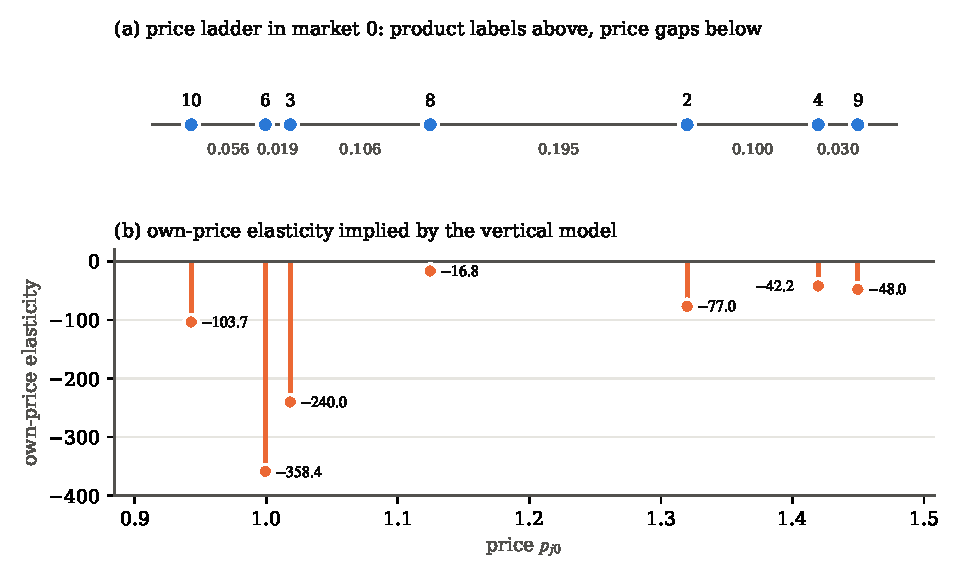
\includegraphics[width=0.9\linewidth]{figures/appC/ladder.pdf}
\caption{The price ladder in market 0. Panel (a) shows the seven prices with the gaps between neighbours. Panel (b)
shows the own-price elasticity $\varepsilon_{jj}$ that the vertical model implies for each product. The products with
the closest neighbours, 6 and 3, have the largest elasticities.}
\label{fig:C-ladder}
\end{figure}

The ladder also governs substitution to the outside good. In the vertical model only the cheapest product loses
customers to the outside good when its price rises. The diversion ratio from product $k$ to the outside good is
\[
  D_{k0} = -\frac{\partial s_0}{\partial p_k}\Big(\frac{\partial s_k}{\partial p_k}\Big)^{-1},
\]
the fraction of the sales that $k$ loses which go to the outside good. For product 10 it is 0.064. Every other product diverts
nothing to the outside good. The logit of \cref{sec:C-logit-est} puts these diversion ratios between 0.86 and 0.91, much
closer to the true model, in which most consumers who leave a product stop buying yogurt (\cref{sec:C-rc-est}).

\casehead{Part (f)}
The vertical model is appropriate when products differ mainly along one quality dimension that all consumers value in
the same direction. Consumers should differ mainly in income or in their marginal utility of money. Then the price
ladder is a quality ladder, and neighbours on it are the natural substitutes. \citet{Bresnahan1987} uses this structure
for the 1955 automobile price war. His consumers have utility $U = vx + Y - P$ from a car of quality $x$ and price $P$,
with $v$ uniform on $[0, V_{\max}]$ with density $d$ (eq.~1, p.~460, and p.~461). Bresnahan writes $\delta$ for
this density. The demand for a car between
neighbours $h$ and $j$ is linear in prices,
\[
  q_i = d\Big[\frac{P_j - P_i}{x_j - x_i} - \frac{P_i - P_h}{x_i - x_h}\Big]
\]
(eq.~5, p.~462). He notes that the quality difference $x_i - x_h$ measures how close two products are as substitutes,
and that they become perfect substitutes as $x_i$ approaches $x_h$ (p.~462). The same feature produces the large
elasticities of \cref{tab:C-velast}. Bresnahan also shows that demand in this model is continuous and concave across the
point where a neighbour is priced out, so a price equilibrium always exists (footnote~6, p.~462). Because only neighbours
compete, collusive and Nash pricing imply very different markups, which gives his conduct test its power
(\cref{sec:06-bresnahan}). The fact to explain is that 1955 production was 45 percent above that of the two surrounding
years, while quality-adjusted prices were lower (p.~457). In nonnested Cox tests the collusive solution is sustained in
1954 and 1956, and the competitive (Nash) solution in 1955 (abstract, p.~457).

Our simulated market violates the premises. Tastes vary along four dimensions, the products crowd into a narrow price
range, and the outside good takes more than three quarters of every market. The vertical model can explain why consumers
split across products with similar prices only by placing those products almost on top of one another in quality. It
then reads every small price gap as intense competition. Its elasticities are wrong by one to two orders of magnitude,
its markups are close to zero, and its implied costs absorb the error. The data offer two warning signs even without
knowledge of the truth. Qualities explain almost none of their own variation ($R^2 = 0.015$), and the implied Nash
markups are far below what any plausible cost information would allow. A model with an idiosyncratic shock, such as
the logit of \cref{sec:C-logit-est}, avoids the zero cross elasticities by construction.

\subsection{Computational notes}

The computations take a few seconds in total.
\begin{enumerate}
  \item In each market, sort products by price and form $\bar S_{(k)t}$ as reversed cumulative sums of the sorted
  realized shares.
  \item Compute $y_{jt}$ by \eqref{eq:C-vy} with \texttt{log1p} for $\ln(1 - \bar S)$, and run OLS of $y$ on $x$ with the
  clustered variance \eqref{eq:C-clustervar}.
  \item Compute $g_{(k)t}$ from \cref{cor:C-vfree}, fill the tridiagonal $\Delta_t$, form $\Omega_t$ from the owners and
  solve $(\Omega_t \odot \Delta_t^\top)\,a = s_t$ for the markups $-a$.
  \item Check the derivatives with a complex step, and check that the shares implied by the recovered qualities
  reproduce the data (largest error $1.9\times10^{-14}$).
\end{enumerate}
The inversion takes a few lines of code.
\begin{verbatim}
def vertical_delta(p, s, lam):
    order = np.argsort(p)                       # price ladder
    tail = np.cumsum(s[order][::-1])[::-1]      # bar S_(k)
    steps = np.diff(p[order], prepend=0.0)      # p_(k) - p_(k-1)
    delta = np.empty_like(p)
    delta[order] = np.cumsum(steps * -np.log1p(-tail) / lam)
    return delta
\end{verbatim}

\section{Estimating logit demand and recovering costs}\label{sec:C-logit-est}

The logit model becomes a linear regression once shares are inverted, so all the tools of linear instrumental variables
apply. In this problem we estimate it on the simulated market, study the strength of the usual instruments, recover
marginal costs with correct standard errors, and estimate demand and supply jointly. Since the data come from a random
coefficients model, the logit is misspecified. We close by deriving the bias that omitted taste heterogeneity creates in
the logit price coefficient and by measuring it in the simulated sample. The general theory of logit estimation is in \cref{ch:logit}.

\subsection{Statement}

Use the data and \cref{ass:C-est} of \cref{sec:C-vertical}. Demand is now logit:
\begin{equation}\label{eq:C-logit}
  u_{ijt} = \delta^l_{jt} + \epsilon_{ijt}, \qquad \delta^l_{jt} = x_{jt}\beta^l - \alpha^l p_{jt} + \xi_{jt},
\end{equation}
with $\epsilon_{ijt}$ independent type-I extreme value and $u_{i0t} = \epsilon_{i0t}$. Firms set prices in a
multi-product Bertrand-Nash equilibrium.

\begin{enumerate}[label=(\alph*)]
  \item Estimate $(\beta^l, \alpha^l)$. Give the identification argument, justify the instruments, assess their strength
  and report standard errors.
  \item Compute the elasticity matrix for market 0 and discuss it.
  \item Derive the marginal cost equation under the assumed conduct, compute $mc_{jt}$ and estimate
  $(\gamma_1, \gamma_2)$ with standard errors that account for the estimation of $\alpha^l$.
  \item Explain how to estimate demand and supply jointly, and when joint estimation matters. Carry it out.
  \item The true model has a random coefficient on price. Show why the logit price coefficient is then biased even with
  valid instruments, explain why the bias is toward zero in this design, and measure it.
\end{enumerate}

\subsection{Solution}

\casehead{Part (a)}
With logit demand the inside and outside shares are
\[
  s_{jt} = \frac{e^{\delta^l_{jt}}}{1 + \sum_{k}e^{\delta^l_{kt}}}, \qquad s_{0t} = \frac{1}{1 + \sum_{k}e^{\delta^l_{kt}}} .
\]
Dividing the first by the second gives $\frac{s_{jt}}{s_{0t}} = e^{\delta^l_{jt}}$, and taking logs gives the inversion of
\citet[eq.~14, p.~250]{Berry1994},
\begin{equation}\label{eq:C-berry}
  \ln s_{jt} - \ln s_{0t} = x_{jt}\beta^l - \alpha^l p_{jt} + \xi_{jt}.
\end{equation}
The left side is computed from realized shares, with $s_{0t} = 1 - \sum_j s_{jt}$. Equation \eqref{eq:C-berry} is
linear in the parameters, with the unobserved quality $\xi_{jt}$ as its error (\cref{eq:07-logit-inversion}).

Price is endogenous. Firms observe $\xi_{jt}$ when they set prices. A product with higher unobserved quality has a
larger share, and logit markups rise with the firm's share (part (c)), so $\Cov(p_{jt}, \xi_{jt}) > 0$. Let
$\tilde p_{jt}$ be the residual from projecting price on $x_{jt}$. The OLS estimate of the price coefficient then converges
to $-\alpha^l + \frac{\Cov(\tilde p_{jt}, \xi_{jt})}{\Var(\tilde p_{jt})}$, so OLS biases $\alpha^l$ toward zero
(\cref{prop:07-ols-bias}). We need excluded instruments that move price and are uncorrelated with $\xi_{jt}$.

We use seven excluded instruments.
\begin{enumerate}
  \item The price of milk $w_{jt}$. It shifts marginal cost and therefore price, it is excluded from utility, and it is
  independent of $\xi_{jt}$ by \cref{ass:C-est}(iii).
  \item Characteristics of the other products in the market. For each characteristic $k$ of product $j$ owned by firm $f$,
  \citet[eq.~5.8, p.~861]{BerryLevinsohnPakes1995} use the sums $\sum_{r \ne j, r \in \mathcal{J}_f}x_{rk}$ and
  $\sum_{r \notin \mathcal{J}_f}x_{rk}$. We form these sums for sugar content and the organic indicator. Because one
  characteristic is the constant, the numbers of the firm's other products and of rival products, $n^{own}_{jt}$ and
  $n^{riv}_{jt}$, are instruments too. This gives six instruments.
\end{enumerate}
\citet[p.~249]{Berry1994} explains why the second group is valid. Rival characteristics are excluded from $u_{ijt}$, and
they are correlated with prices through the markups in the first-order conditions. Their validity requires that
characteristics and the set of products offered in each market be independent of $\xi_{jt}$, which we add to
\cref{ass:C-est}. In this design characteristics are fixed by product, so the six instruments vary only through
which products a market offers and who owns them. The number of the firm's other products runs from 0 to 3 (mean 1.37),
and the number of rival products from 1 to 8 (mean 4.55).

The parameters $\theta^l = (\beta^l, \alpha^l)$ are identified by the moment conditions
\begin{equation}\label{eq:C-logit-moments}
  \E\big[z_{jt}^\top\xi_{jt}\big] = 0, \qquad z_{jt} = \big(x_{jt}, w_{jt}, \text{six competition instruments}\big),
\end{equation}
together with the rank condition that $\E[z_{jt}^\top(x_{jt}, p_{jt})]$ has full column rank four. Economically,
variation in price that comes from costs and from competition, and is unrelated to unobserved quality, traces out how
shares respond to price. We estimate by \emph{two-stage least squares} (2SLS). With $Y$ the stacked left side of
\eqref{eq:C-berry}, $X = (x, p)$ and $Z$ the instrument matrix, the 2SLS coefficient vector is
\[
  \hat b^l = (\hat X^\top\hat X)^{-1}\hat X^\top Y, \qquad \hat X = Z(Z^\top Z)^{-1}Z^\top X .
\]
Since price enters \eqref{eq:C-berry} with coefficient $-\alpha^l$, $\hat b^l$ estimates $(\beta^l, -\alpha^l)$. Its first
three entries give $\hat\beta^l$, and $\hat\alpha^l$ is minus its price entry. The clustered variance of $\hat b^l$ is
\eqref{eq:C-clustervar} with $X_t$ replaced by $\hat X_t$. The residuals in the middle factor are the 2SLS residuals
$\hat e_t = Y_t - X_t\hat b^l$, computed with the actual regressors (\cref{app:econometrics}).

\Cref{tab:C-firststage} reports the first stage. Instrument strength comes almost entirely from the milk price,
whose coefficient is 0.497 with standard error 0.026, close to the true cost coefficient of 0.5. The cluster-robust Wald
statistic for the seven excluded instruments, divided by seven, is 92.5. With one endogenous regressor this is the
cluster-robust first-stage $F$ statistic of \citet{KleibergenPaap2006}. The homoskedastic $F$ is 74.1 and the partial $R^2$ is
0.446. The milk price alone gives $F = 591.4$. The six competition instruments are jointly weak, with $F = 2.32$ and
$p = 0.039$ given the milk price.

\begin{table}[htbp]
\centering
\caption{First stage: OLS of $p_{jt}$ on the exogenous variables}
\label{tab:C-firststage}
\small
\begin{tabular}{@{}lcc@{}}
\toprule
 & Coefficient & Standard error \\
\midrule
Constant & 0.5778 & (0.0188) \\
Sugar content & 0.2575 & (0.0113) \\
Organic & 0.3138 & (0.0064) \\
Price of milk $w_{jt}$ & 0.4972 & (0.0256) \\
Sugar, firm's other products & 0.0023 & (0.0106) \\
Sugar, rival products & $-0.0042$ & (0.0077) \\
Organic, firm's other products & $-0.0015$ & (0.0068) \\
Organic, rival products & $-0.0009$ & (0.0040) \\
Number of firm's other products & 0.0038 & (0.0116) \\
Number of rival products & 0.0020 & (0.0084) \\
\midrule
$R^2$ & 0.923 & \\
$F$, seven excluded instruments (cluster-robust) & 92.5 & \\
$F$, seven excluded instruments (homoskedastic) & 74.1 & \\
$F$, six competition instruments (cluster-robust) & 2.32 & \\
$F$, milk price only (cluster-robust) & 591.4 & \\
\bottomrule
\end{tabular}

\vspace{3pt}
\begin{minipage}{0.97\textwidth}
\footnotesize Notes: 654 observations. Standard errors clustered by market. The milk-price-only
statistic comes from the regression of price on $(x_{jt}, w_{jt})$.
Computed with \texttt{figures/appC/src/appC\_vertical\_logit.py}.
\end{minipage}
\end{table}

The competition instruments are weak for two reasons. First, logit markups barely respond to competition in this
market. The markup of firm $f$ is $\frac{1}{\alpha^l(1 - S_{ft})}$ (part (c)), and the largest combined share of a
firm is only 0.112, so the implied markups run from 0.379 to 0.426. Changes in the set of competitors cannot move prices
much. Second, the instruments are nearly collinear. Sugar content varies only from 0.64 to 1.35, so each sum of sugar
is close to a multiple of the corresponding count. The correlations are 0.978 for the firm's own products and 0.988 for
rivals. The variance inflation factors of the two sugar sums and the two counts are 40.1, 57.8, 36.1 and 52.2. A
variance inflation factor is $\frac{1}{1 - R_k^2}$, the factor by which collinearity with the other regressors inflates
the variance of coefficient $k$.
\citet[p.~861]{BerryLevinsohnPakes1995} report the same problem, finding the matrix of these linear terms ``nearly not
of full rank.''

\Cref{tab:C-logit-demand} reports the estimates. As expected, OLS gives a smaller price coefficient, 2.330, than 2SLS,
2.641. Hansen's test of the six overidentifying restrictions \citep{Hansen1982} uses the two-step GMM estimator with a
market-clustered weighting matrix. It does not reject, with $J = 8.82$ and $p = 0.18$. The two-step GMM estimate of the
price coefficient is 2.872. With the milk price as the only excluded instrument, 2SLS gives 2.677 (0.415), so the
competition instruments change little.

\begin{table}[htbp]
\centering
\caption{Logit demand estimates}
\label{tab:C-logit-demand}
\small
\begin{tabular}{@{}lcccc@{}}
\toprule
 & OLS & 2SLS & \makecell{2SLS,\\ milk price only} & True \\
\midrule
Constant & $-1.443$ & $-1.184$ & $-1.154$ & $-1.00$ \\
 & (0.226) & (0.329) & (0.334) & \\
Sugar content & 0.119 & 0.190 & 0.198 & 0.20 \\
 & (0.122) & (0.158) & (0.156) & \\
Organic & 0.051 & 0.153 & 0.165 & 0.15 \\
 & (0.097) & (0.141) & (0.142) & \\
Price coefficient $\alpha^l$ & 2.330 & 2.641 & 2.677 & 3.00 \\
 & (0.252) & (0.412) & (0.415) & \\
\midrule
First-stage $F$ (cluster-robust) & & 92.5 & 591.4 & \\
Hansen $J$ ($p$-value) & & 8.82 (0.18) & & \\
$R^2$ & 0.396 & 0.395 & 0.395 & \\
Observations & 654 & 654 & 654 & \\
\bottomrule
\end{tabular}

\vspace{3pt}
\begin{minipage}{0.97\textwidth}
\footnotesize Notes: Dependent variable $\ln s_{jt} - \ln s_{0t}$. Standard errors clustered by
market in parentheses. The table reports $\alpha^l$, minus the coefficient on price. The true values are the mean
parameters of the random coefficients model of \cref{sec:C-simulate}.
Computed with \texttt{figures/appC/src/appC\_vertical\_logit.py}.
\end{minipage}
\end{table}

Consistency of 2SLS here rests on one more condition. Characteristics and milk prices are fixed by product, so the
identifying variation in $w_{jt}$ comes from its ten values across products. If $\xi_{jt}$ contained a persistent
product component, it could correlate with the product-level instruments. An $F$ test of product dummies on the 2SLS
residuals, beyond the product-level regressors, gives $F(6, 644) = 1.18$ with $p = 0.32$. With only ten products the test
has little power, so it cannot rule such a component out. In this design the unobservables are drawn independently
across markets, so the condition holds by construction.

The 2SLS price coefficient, 2.641, lies below the true mean of 3, but only 0.87 standard errors below. The
characteristic coefficients are close to the truth and imprecise, because sugar and organic status take only ten distinct
combinations. Part (e) splits the shortfall in $\hat\alpha^l$. Most of it, 0.284 of 0.359, is an estimate of the
misspecification bias of the logit. The rest reflects sampling and simulation error, since the random coefficients model
gives 2.926 on the same sample.

\casehead{Part (b)}
The logit share derivatives of \cref{sec:C-logit-bertrand}, part (a), hold with $\alpha^l$ in place of $\alpha$
(\cref{prop:07-logit-derivs}). They give the elasticities \eqref{eq:C-logit-elast} together with the outside-good row,
\begin{equation}\label{eq:C-lelast}
  \varepsilon_{jj} = -\alpha^l p_j(1 - s_j), \qquad \varepsilon_{jk} = \alpha^l p_ks_k \quad (k \ne j), \qquad
  \varepsilon_{0k} = \alpha^l p_ks_k .
\end{equation}
\Cref{tab:C-lelast} evaluates them at $\hat\alpha^l = 2.641$ and the observed prices and realized shares of market 0.

\begin{table}[htbp]
\centering
\caption{Logit model: price elasticities in market 0}
\label{tab:C-lelast}
\small
\begin{tabular}{@{}lrrrrrrr@{}}
\toprule
 & \multicolumn{7}{c}{Price of product} \\
\cmidrule(lr){2-8}
Share of & 2 & 3 & 4 & 6 & 8 & 9 & 10 \\
\midrule
Product 2 & $-3.47$ & 0.07 & 0.05 & 0.05 & 0.17 & 0.02 & 0.05 \\
Product 3 & 0.02 & $-2.62$ & 0.05 & 0.05 & 0.17 & 0.02 & 0.05 \\
Product 4 & 0.02 & 0.07 & $-3.70$ & 0.05 & 0.17 & 0.02 & 0.05 \\
Product 6 & 0.02 & 0.07 & 0.05 & $-2.59$ & 0.17 & 0.02 & 0.05 \\
Product 8 & 0.02 & 0.07 & 0.05 & 0.05 & $-2.80$ & 0.02 & 0.05 \\
Product 9 & 0.02 & 0.07 & 0.05 & 0.05 & 0.17 & $-3.81$ & 0.05 \\
Product 10 & 0.02 & 0.07 & 0.05 & 0.05 & 0.17 & 0.02 & $-2.44$ \\
Outside good & 0.02 & 0.07 & 0.05 & 0.05 & 0.17 & 0.02 & 0.05 \\
\bottomrule
\end{tabular}

\vspace{3pt}
\begin{minipage}{0.97\textwidth}
\footnotesize Notes: Entry $(j, k)$ is $\varepsilon_{jk}$ from \eqref{eq:C-lelast} with
$\hat\alpha^l = 2.641$ (2SLS), evaluated at observed prices and realized shares. Computed with \texttt{figures/appC/src/appC\_vertical\_logit.py}.
\end{minipage}
\end{table}

The own elasticities run from $-2.44$ to $-3.81$, so every product faces elastic demand. Across all 654 observations
they lie between $-2.21$ and $-4.24$, with mean $-3.06$. They are close to the true values, $-2.57$ to $-3.85$ in market
0, but slightly smaller in magnitude, because $\hat\alpha^l$ is below 3. Since shares are small,
$\varepsilon_{jj} \approx -\alpha^l p_j$, so the model makes the most expensive products the most elastic by
construction. Products 9 and 4, the two most expensive, have the largest own elasticities.

Every off-diagonal entry in a column is the same, and it equals the outside-good entry. This is the independence of
irrelevant alternatives. A rise in $p_k$ raises the shares of all other products and of the outside good in the same
proportion, whatever their characteristics. Diversion from product $k$ to the outside good is
$D_{k0} = \frac{\alpha^l s_0s_k}{\alpha^l s_k(1 - s_k)} = \frac{s_0}{1 - s_k}$, between 0.86 and 0.91 in market 0. In the
true model a price rise for an organic product diverts more customers to the other organic products and to expensive
products (\cref{sec:C-rc-est}). The logit cannot produce this pattern.

\casehead{Part (c)}
With logit demand the first-order conditions \eqref{eq:C-vsupply-nash} reduce to the common-markup rule of
\cref{prop:C-common-markup}, derived in \cref{sec:C-logit-bertrand}, part (e) (see also \cref{prop:07-logit-multi}).
Every product of firm $f$ in market $t$ carries the markup $m_{ft} = \frac{1}{\alpha^l(1 - S_{ft})}$, where
$S_{ft} = \sum_{k \in \mathcal{J}_{ft}}s_{kt}$ is the firm's combined share. The marginal cost equation is
\begin{equation}\label{eq:C-lsupply}
  mc_{jt} = p_{jt} - \frac{1}{\alpha^l(1 - S_{ft})} = x_{jt}\gamma_1 + \gamma_2 w_{jt} + \omega_{jt} .
\end{equation}
This is \eqref{eq:C-vsupply-nash} with the logit Jacobian. The script confirms that the closed form and the matrix formula
agree to $2.2\times10^{-16}$. We compute $mc_{jt}$ with $\hat\alpha^l = 2.641$ and the realized shares. The implied
markups run from 0.379 to 0.426 with mean 0.396, against a true mean of 0.386. Their correlation with the true markups
is 0.55, against 0.27 for the vertical Nash markups. No implied marginal cost is negative. Identification of
$(\gamma_1, \gamma_2)$ follows as in \cref{sec:C-vertical}, from $\E[\omega_{jt} \mid x_{jt}, w_{jt}] = 0$ and full rank.
We estimate it by OLS of $mc_{jt}$ on $(x_{jt}, w_{jt})$.

The dependent variable now contains the estimate $\hat\alpha^l$. Clustered OLS standard errors treat $mc_{jt}$ as data
and so ignore this uncertainty. We correct them in two ways.

The first is a \emph{market bootstrap}. Each of 5,000 replications draws 100 markets with replacement, re-estimates
$(\beta^l, \alpha^l)$ by 2SLS, recomputes every implied marginal cost with the new $\alpha^l$, and re-runs the supply
regression. The bootstrap standard error is the standard deviation of the replicated estimates. Resampling whole markets
preserves dependence within markets and is valid because markets are independent. With 5,000 replications the Monte
Carlo error of each bootstrap standard error of the cost coefficients is below 0.0011.

The second treats the two steps as one GMM estimator with stacked moments \citep{Newey1984, MurphyTopel1985}. Write
$k_{jt} = \frac{1}{1 - S_{ft}}$, so that $mc_{jt}(\alpha) = p_{jt} - \frac{k_{jt}}{\alpha}$, and let $W$ be the regressor
matrix of \eqref{eq:C-supplydecomp}, with rows $W_{jt} = (x_{jt}, w_{jt})$. The supply estimate solves
$\sum_{t}\sum_j W_{jt}^\top\big(p_{jt} - \frac{k_{jt}}{\hat\alpha^l} - W_{jt}\hat\gamma\big) = 0$. A first-order expansion
around the probability limits gives
\begin{equation}\label{eq:C-stacked}
  \begin{aligned}
  \hat\gamma - \gamma &\approx (W^\top W)^{-1}\Big[\sum_{t}\sum_j W_{jt}^\top\omega_{jt}
  + \frac{W^\top k}{(\alpha^l)^2}\big(\hat\alpha^l - \alpha^l\big)\Big], \\
  \hat\alpha^l - \alpha^l &\approx -\iota_p^\top(\hat X^\top\hat X)^{-1}\sum_{t}\sum_j\hat X_{jt}^\top\xi_{jt},
  \end{aligned}
\end{equation}
where $\iota_p$ selects the price coefficient. Each observation thus contributes an influence term to $\hat\gamma$.
Summing these terms within markets and taking the clustered outer product gives a sandwich variance that includes the
estimation error in $\alpha^l$. The coefficient $(W^\top W)^{-1}\frac{W^\top k}{(\alpha^l)^2}$ measures how the cost estimates
move with $\alpha^l$. For the constant it is 0.148, close to the mean markup divided by $\alpha^l$. With
$\text{s.e.}(\hat\alpha^l) = 0.412$, this alone gives a standard error of about $0.148 \times 0.412 = 0.061$ for the
intercept. \Cref{tab:C-lsupply} reports the estimates.

\begin{table}[htbp]
\centering
\caption{Logit model, supply side: OLS of the implied marginal cost on $(x_{jt}, w_{jt})$}
\label{tab:C-lsupply}
\small
\setlength{\tabcolsep}{5pt}
\begin{tabular}{@{}lcccccc@{}}
\toprule
 & Estimate & \makecell{Clustered\\ s.e.} & \makecell{Stacked\\ s.e.} & \makecell{Bootstrap\\ s.e.}
 & \makecell{Bootstrap\\ 95\% interval} & True \\
\midrule
Constant & 0.160 & 0.016 & 0.065 & 0.072 & $[-0.022, 0.257]$ & 0.20 \\
Sugar content & 0.258 & 0.010 & 0.010 & 0.010 & $[0.239, 0.278]$ & 0.25 \\
Organic & 0.315 & 0.005 & 0.006 & 0.006 & $[0.304, 0.327]$ & 0.30 \\
Price of milk & 0.532 & 0.023 & 0.023 & 0.023 & $[0.487, 0.576]$ & 0.50 \\
\bottomrule
\end{tabular}

\vspace{3pt}
\begin{minipage}{0.97\textwidth}
\footnotesize Notes: The implied marginal cost is \eqref{eq:C-lsupply} with $\hat\alpha^l = 2.641$, and
$R^2 = 0.923$. The clustered standard errors treat $mc_{jt}$ as data. The stacked standard errors use the influence
functions in \eqref{eq:C-stacked}, clustered by market. The bootstrap resamples markets 5,000 times and re-estimates
$\alpha^l$ in each replication. The interval is the percentile interval.
Computed with \texttt{figures/appC/src/appC\_vertical\_logit.py}.
\end{minipage}
\end{table}

The estimates are close to the true values. Uncertainty about $\alpha^l$ moves all markups together, since each is near
$\frac{1}{\alpha^l}$ when shares are small. It therefore loads almost entirely on the intercept, whose standard error rises
from 0.016 to 0.065 (stacked) or 0.072 (bootstrap), while the slope standard errors barely change. The two corrections
agree closely. The decomposition \eqref{eq:C-supplydecomp} locates the remaining errors. The logit markup error loads
$-0.040$ on the constant, $0.011$ on sugar, $0.011$ on organic and $0.030$ on the milk price. True markups are higher for
organic products (0.392 against 0.383), because their buyers are less price sensitive. Logit markups are slightly lower
for them (0.392 against 0.397), because organic producers have smaller combined shares. The logit therefore understates
the organic markup premium ($-0.005$ against $+0.008$ in the truth), so it overstates the organic cost premium. The
bootstrap interval for the organic coefficient just excludes 0.30.
Compared with the vertical model under Nash pricing (\cref{tab:C-vsupply}), the logit recovers costs far more accurately
because its markups are close to the true ones.

\casehead{Part (d)}
Joint estimation stacks the demand and supply moments and estimates
$\theta = (\beta^l, \alpha^l, \gamma_1, \gamma_2)$ by GMM. For a candidate $\theta$, the residuals are
\begin{equation}\label{eq:C-joint-resid}
  \xi_{jt}(\theta) = \ln s_{jt} - \ln s_{0t} - x_{jt}\beta^l + \alpha^l p_{jt}, \qquad
  \omega_{jt}(\theta) = p_{jt} - \frac{1}{\alpha^l(1 - S_{ft})} - x_{jt}\gamma_1 - \gamma_2 w_{jt}.
\end{equation}
With demand instruments $z^d_{jt}$ and supply instruments $z^s_{jt}$, the sample moments and the estimator are
\begin{equation}\label{eq:C-joint}
  \bar g(\theta) = \frac{1}{N}\sum_{t}\sum_j\begin{pmatrix} z^{d\top}_{jt}\,\xi_{jt}(\theta) \\
  z^{s\top}_{jt}\,\omega_{jt}(\theta)\end{pmatrix}, \qquad
  \hat\theta = \argmin_\theta \bar g(\theta)^\top\,\mathcal W\,\bar g(\theta).
\end{equation}
The first step uses the block-diagonal weight $\mathcal W_1 = \diag\big((\frac{1}{N}Z^{d\top}Z^d)^{-1},
(\frac{1}{N}Z^{s\top}Z^s)^{-1}\big)$. The second step uses the inverse of the market-clustered covariance of the moments
at the first-step estimate, $\mathcal W_2 = \hat S^{-1}$, which is efficient. Given $\alpha^l$, both residuals are linear in
$(\beta^l, \gamma_1, \gamma_2)$, so we concentrate these out by weighted least squares and search over $\alpha^l$ alone.
The GMM sandwich then gives standard errors that account for the estimation of $\alpha^l$ in the markups
(\cref{sec:08-supply-joint}).

\begin{proposition}[A just-identified supply block adds nothing]\label{prop:C-redundant}
Let $z^s_{jt} = (x_{jt}, w_{jt})$, so that the supply block has as many moments as cost parameters. Then the joint GMM
estimate of $(\beta^l, \alpha^l)$ with weight $\mathcal W$ equals the GMM estimate from the demand moments alone with weight
$\mathcal W_{dd} - \mathcal W_{ds}\mathcal W_{ss}^{-1}\mathcal W_{sd}$. With the block-diagonal $\mathcal W_1$ this is 2SLS. With
the efficient $\mathcal W_2 = \hat S^{-1}$ it is two-step efficient GMM on the demand moments with weight $\hat S_{dd}^{-1}$.
\end{proposition}

\begin{proof}
Partition $\bar g = (\bar g_d, \bar g_s)$. For fixed $(\beta^l, \alpha^l)$, $\bar g_s = b_s(\alpha^l) - \frac{1}{N}W^\top
W\gamma$, and $\frac{1}{N}W^\top W$ is square and invertible. Choosing $\gamma$ is therefore the same as choosing the value
$v$ of $\bar g_s$ freely. Minimizing the quadratic form over $v$,
\[
  \min_v\begin{pmatrix}\bar g_d \\ v\end{pmatrix}^\top
  \begin{pmatrix}\mathcal W_{dd} & \mathcal W_{ds} \\ \mathcal W_{sd} & \mathcal W_{ss}\end{pmatrix}
  \begin{pmatrix}\bar g_d \\ v\end{pmatrix}
  = \bar g_d^\top\big(\mathcal W_{dd} - \mathcal W_{ds}\mathcal W_{ss}^{-1}\mathcal W_{sd}\big)\bar g_d ,
\]
attained at $v = -\mathcal W_{ss}^{-1}\mathcal W_{sd}\bar g_d$. The concentrated objective involves only the demand
moments. For block-diagonal $\mathcal W$ the bracket is $\mathcal W_{dd}$. For $\mathcal W = \hat S^{-1}$, the formula for the
inverse of a partitioned matrix gives $\mathcal W_{dd} - \mathcal W_{ds}\mathcal W_{ss}^{-1}\mathcal W_{sd} = \hat S_{dd}^{-1}$.
\end{proof}

This is a special case of a general separability result for GMM \citep{AhnSchmidt1995}. The supply side carries
information about demand only when it has more moments than cost parameters. Under \cref{ass:C-est}(iii), $\omega_{jt}$ is
also independent of the characteristics of other products, so the six competition instruments are valid supply
instruments. \citet[p.~255]{Berry1994} proposes the characteristics of other firms as cost-side instruments for the same
reason. \citet[pp.~861--862]{BerryLevinsohnPakes1995} interact their cost error with the three terms of their eq.~(5.8)
for each of six cost characteristics. The three terms are the characteristic itself, its sum over the firm's other
products and its sum over rival products. They add miles per dollar, a demand variable excluded from cost, for nineteen cost-side
instruments in all.

With these instruments the supply equation identifies $\alpha^l$ on its own. Rewrite \eqref{eq:C-lsupply} as
\begin{equation}\label{eq:C-supply-only}
  p_{jt} = x_{jt}\gamma_1 + \gamma_2 w_{jt} + \frac{1}{\alpha^l}\,k_{jt} + \omega_{jt}, \qquad k_{jt} = \frac{1}{1 - S_{ft}} ,
\end{equation}
a linear regression in which $\frac{1}{\alpha^l}$ is the coefficient on $k_{jt}$. This is the multi-product version of the
logit supply equation of \citet[eq.~31, p.~255]{Berry1994}, whose parameters are $\gamma$ and $\frac{1}{\alpha}$. The firm
share is endogenous, because a high $\omega_{jt}$ raises the price and lowers the share. The competition instruments predict
$k_{jt}$ well, with a cluster-robust first-stage $F$ of 51.6. The number and type of a firm's other products move its
combined share directly. 2SLS of \eqref{eq:C-supply-only} gives $\frac{1}{\hat\alpha^l} = 0.351$ (0.132), so
$\hat\alpha^l = 2.85$ with a delta-method standard error of 1.07. The estimate is close to the demand-side values, but it
is imprecise because $k_{jt}$ varies only from 1.002 to 1.126. The markups move too little across markets to measure their
slope well. \Cref{tab:C-joint} shows what the joint estimator does with this extra information.

\begin{table}[htbp]
\centering
\caption{Sequential and joint estimation of logit demand and supply}
\label{tab:C-joint}
\small
\begin{tabular}{@{}lcccc@{}}
\toprule
 & Sequential & \makecell{Joint GMM,\\ $z^s = (x, w)$} & \makecell{Joint GMM, $z^s$ adds\\ six instruments}
 & True \\
\midrule
\multicolumn{5}{l}{\textit{Demand}} \\
Constant & $-1.184$ (0.329) & $-1.035$ (0.311) & $-1.101$ (0.291) & $-1.00$ \\
Sugar content & 0.190 (0.158) & 0.291 (0.152) & 0.267 (0.144) & 0.20 \\
Organic & 0.153 (0.141) & 0.211 (0.134) & 0.178 (0.123) & 0.15 \\
Price coefficient $\alpha^l$ & 2.641 (0.412) & 2.872 (0.394) & 2.785 (0.367) & 3.00 \\
\multicolumn{5}{l}{\textit{Marginal cost}} \\
Constant & 0.160 (0.072) & 0.191 (0.053) & 0.181 (0.053) & 0.20 \\
Sugar content & 0.258 (0.010) & 0.261 (0.010) & 0.260 (0.009) & 0.25 \\
Organic & 0.315 (0.006) & 0.315 (0.005) & 0.314 (0.005) & 0.30 \\
Price of milk & 0.532 (0.023) & 0.529 (0.022) & 0.527 (0.021) & 0.50 \\
\midrule
Moments & & 14 & 20 & \\
Hansen $J$ (d.f., $p$) & & 8.82 (6, 0.18) & 12.85 (12, 0.38) & \\
\bottomrule
\end{tabular}

\vspace{3pt}
\begin{minipage}{0.97\textwidth}
\footnotesize Notes: The sequential column is 2SLS for demand (clustered standard errors) and OLS
for supply (bootstrap standard errors). The joint columns are two-step efficient GMM estimates of \eqref{eq:C-joint} with
$z^d$ as in part (a), weights clustered by market, and GMM sandwich standard errors without a small-sample factor. With
$z^s = (x, w)$ the first step reproduces the sequential point estimates (\cref{prop:C-redundant}). With the six added
supply instruments the first step gives $\hat\alpha^l = 2.642$, which differs slightly from the sequential 2.641.
Computed with \texttt{figures/appC/src/appC\_vertical\_logit.py}.
\end{minipage}
\end{table}

The numbers confirm \cref{prop:C-redundant}. With $z^s = (x, w)$, the first-step joint estimate of $\alpha^l$ is 2.641, the
2SLS value. The second-step estimate is 2.872, exactly the two-step GMM estimate from the demand moments alone, and the
$J$ statistic is the same 8.82. The cost coefficients do change, because the efficient weight lets demand residuals inform
the supply block. Adding the six competition instruments to the supply side changes even the first step, which gives
2.642. The cost parameters can no longer set every supply moment to zero, and the remaining supply moments depend on
$\alpha^l$ through the markups. The second step gives $\hat\alpha^l = 2.785$ with standard error 0.367, against 0.394
without the added instruments. The estimate is close to the demand-side estimates and to the supply-only value of
2.85. The gain in precision is modest, for the reason that made these instruments weak in the first stage. With combined shares
of at most 0.112, the markups barely change with competition. The overidentifying restrictions are not rejected
($J = 12.85$ with 12 degrees of freedom, $p = 0.38$).

Joint estimation matters in four situations. The first is when demand moments identify the demand parameters poorly,
because instruments are weak or because there are nonlinear parameters such as the random coefficients of
\cref{sec:C-rc-est}. Extra supply moments then add information. The second is when $\xi_{jt}$ and $\omega_{jt}$ are
correlated and the supply block is overidentified, since the efficient weight then links the blocks. The third is when
conduct itself is a parameter, because only the supply side identifies it. The fourth is when correct standard errors for
the cost parameters are needed and no bootstrap is run. Joint estimation also has a cost. If the conduct assumption is
wrong, the supply moments contaminate the demand estimates, which sequential estimation protects against.

\casehead{Part (e)}
The true model of \cref{sec:C-simulate} has random coefficients, $u_{ijt} = \delta_{jt} + \tilde x_{jt}\Sigma\nu_i +
\epsilon_{ijt}$ with $\tilde x_{jt} = (x_{jt}, p_{jt})$, $\nu_i \sim N(0, I_4)$ and $\delta_{jt} = x_{jt}\beta - \alpha
p_{jt} + \xi_{jt}$. Let $\delta_{jt}$ be the mean utility that rationalizes the observed shares in this model, recovered
by the contraction of \cref{thm:08-contraction}, which \cref{prop:C-blp-contraction} of the next problem verifies for
this market. Define the \emph{gap term}
\begin{equation}\label{eq:C-gap}
  r_{jt} = \ln\frac{s_{jt}}{s_{0t}} - \delta_{jt} .
\end{equation}
The logit regression \eqref{eq:C-berry} then has the dependent variable $x_{jt}\beta - \alpha p_{jt} + \xi_{jt} +
r_{jt}$, so its error is $\xi_{jt} + r_{jt}$.

\begin{proposition}[Decomposition of the logit estimate]\label{prop:C-logit-bias}
Use the regressors $(x_{jt}, p_{jt})$ and the instruments $z_{jt}$ throughout. Let $\hat b^{RC}$ be the 2SLS coefficient
vector with dependent variable $\delta_{jt}$, and let $\hat b^l$ be the one with dependent variable $\ln\frac{s_{jt}}{s_{0t}}$.
Write $\hat\alpha^{RC}$ and $\hat\alpha^l$ for minus their price entries. Let $\hat b_r$ be the one with dependent
variable $r_{jt}$, with price coefficient $\hat b_{r,p}$. Then
\begin{equation}\label{eq:C-decomp}
  \hat b^l = \hat b^{RC} + \hat b_r, \qquad \hat\alpha^l = \hat\alpha^{RC} - \hat b_{r,p}.
\end{equation}
Suppose the random coefficients model is correct and $z_{jt}$ is valid for it. Then $\plim\hat\alpha^l = \alpha - b_{r,p}$,
where $b_{r,p}$ is the price coefficient of the population 2SLS projection of $r_{jt}$ on $(x_{jt}, p_{jt})$ with
instruments $z_{jt}$. The logit estimate is biased toward zero whenever $b_{r,p} > 0$.
\end{proposition}

\begin{proof}
The 2SLS estimator is linear in the dependent variable, $\hat b(Y) = (X^\top P_ZX)^{-1}X^\top P_ZY$ with
$P_Z = Z(Z^\top Z)^{-1}Z^\top$. Since $\ln\frac{s_{jt}}{s_{0t}} = \delta_{jt} + r_{jt}$ observation by observation,
$\hat b^l = \hat b(\delta) + \hat b(r) = \hat b^{RC} + \hat b_r$. The price coefficient is $-\alpha$ in both models, so
the price entries give $-\hat\alpha^l = -\hat\alpha^{RC} + \hat b_{r,p}$, which is the second equation. Under the
stated conditions $\plim\hat\alpha^{RC} = \alpha$, and $\hat b_{r,p}$ converges to its population counterpart.
\end{proof}

The instruments do not remove this bias. The gap term depends on prices, and prices depend on the milk price and on the
competition instruments, so $\E[z_{jt}^\top r_{jt}] \ne 0$ in general. The question is the sign of $b_{r,p}$. No general
result fixes it, because it depends on the model, the design and the instruments. The next result shows how $r_{jt}$
varies across the products of one market when tastes are only slightly dispersed.

\begin{proposition}[The gap term for small taste dispersion]\label{prop:C-gap-approx}
Let $\Sigma$ be diagonal and $\nu_i \sim N(0, I_4)$. As $\lVert\Sigma\rVert \to 0$,
\begin{equation}\label{eq:C-gap-approx}
  r_{jt} = \frac{1}{2}\,\tilde x_{jt}\Sigma^2\tilde x_{jt}^\top - \tilde x_{jt}\Sigma^2\bar x_t^\top + O(\lVert\Sigma\rVert^3),
  \qquad \bar x_t = \sum_{k}s_{kt}\tilde x_{kt},
\end{equation}
where the sum runs over inside products. In particular, the price component of $r_{jt}$ is
$\Sigma_{pp}^2\big(\frac{1}{2}p_{jt}^2 - p_{jt}\bar p_t\big)$, with $\Sigma_{pp}$ the price entry of $\Sigma$ and
$\bar p_t = \sum_k s_{kt}p_{kt}$. All products of market $t$ share $\bar p_t$, so among the products of a market priced
above $\bar p_t$ this component is larger for the more expensive product.
\end{proposition}

\begin{proof}
Fix a market and drop $t$. Let $\mu_{ij} = \tilde x_j\Sigma\nu_i$ for inside goods and $\mu_{i0} = 0$. Write
$s^L_j$ for the logit shares at $\delta$, so that $\ln\frac{s^L_j}{s^L_0} = \delta_j$. The individual choice probability is
the logit probability at utilities $\delta_j + \mu_{ij}$. Since $\frac{\partial\ln s_j}{\partial u_k} = \indic\{j = k\} -
s_k$ and $\frac{\partial^2\ln s_j}{\partial u_k\partial u_l} = -s_k(\indic\{k = l\} - s_l)$, a second-order expansion in
$\mu_i$ gives
\[
  \ln s_{ij} = \ln s^L_j + \mu_{ij} - \bar\mu_i - \frac{1}{2}V_i + O(|\mu_i|^3), \qquad
  \bar\mu_i = \sum_k s^L_k\mu_{ik}, \quad V_i = \sum_k s^L_k\mu_{ik}^2 - \bar\mu_i^2 ,
\]
for every alternative, including $j = 0$ with $\mu_{i0} = 0$. Exponentiating and expanding,
\[
  s_{ij} = s^L_j\Big[1 + (\mu_{ij} - \bar\mu_i) - \frac{1}{2}V_i + \frac{1}{2}(\mu_{ij} - \bar\mu_i)^2\Big] + O(|\mu_i|^3).
\]
Average over $\nu_i$. Because $\E[\mu_{ij}] = 0$ and $\mu_i = O(\lVert\Sigma\rVert)$,
\[
  s_j = s^L_j\Big[1 + \frac{1}{2}\E(\mu_{ij} - \bar\mu_i)^2 - \frac{1}{2}\E V_i\Big] + O(\lVert\Sigma\rVert^3), \qquad
  s_0 = s^L_0\Big[1 + \frac{1}{2}\E\bar\mu_i^2 - \frac{1}{2}\E V_i\Big] + O(\lVert\Sigma\rVert^3).
\]
Take logs, use $\ln(1 + a) = a + O(a^2)$ with $a = O(\lVert\Sigma\rVert^2)$, and subtract:
\[
  \ln\frac{s_j}{s_0} - \delta_j = \frac{1}{2}\E\big[(\mu_{ij} - \bar\mu_i)^2 - \bar\mu_i^2\big] + O(\lVert\Sigma\rVert^3)
  = \frac{1}{2}\E[\mu_{ij}^2] - \E[\mu_{ij}\bar\mu_i] + O(\lVert\Sigma\rVert^3).
\]
With $\nu_i \sim N(0, I_4)$ and $\Sigma$ diagonal, $\E[\mu_{ij}^2] = \tilde x_j\Sigma^2\tilde x_j^\top$ and
$\E[\mu_{ij}\bar\mu_i] = \tilde x_j\Sigma^2\big(\sum_k s^L_k\tilde x_k\big)^\top$. Finally $s^L_k - s_k = O(\lVert\Sigma\rVert^2)$,
and the term it multiplies is $O(\lVert\Sigma\rVert^2)$, so replacing $s^L_k$ by $s_k$ changes $r_j$ by $O(\lVert\Sigma\rVert^4)$.
For fixed $\bar p$, the price component $\Sigma_{pp}^2(\frac{1}{2}p^2 - p\bar p)$ has derivative $\Sigma_{pp}^2(p - \bar p)$ in
the product's own price $p$, which is positive for $p > \bar p$.
\end{proof}

The comparison in \cref{prop:C-gap-approx} holds $\bar p_t$ fixed, as it is across the products of one market. It does not
give the response of $r_{jt}$ to a change in $p_{jt}$, which also moves the shares and hence $\bar p_t$. To leading order
the logit share derivatives give $\frac{\partial\bar p_t}{\partial p_{jt}} = s_{jt}\big[1 - \alpha(p_{jt} - \bar p_t)\big]$,
so the full derivative of the price component is
\begin{equation*}
  \Sigma_{pp}^2\Big[(p_{jt} - \bar p_t)(1 + \alpha p_{jt}s_{jt}) - p_{jt}s_{jt}\Big] .
\end{equation*}
It can be negative for a product with a large share. With one inside good, $p = 1$, $\alpha = 1$ and share
$\frac{3}{4}$, it equals $-\frac{5}{16}\Sigma_{pp}^2$, although $p$ exceeds $\bar p = \frac{3}{4}$. Neither derivative
signs $b_{r,p}$ by itself. The 2SLS projection pools products and markets with different $\bar p_t$, and the instruments
decide which price variation it uses. The sign of the bias is therefore specific to the model, the design and the
instruments.

Our design, with small inside shares, is a favorable case for a positive $b_{r,p}$. The outside share is at least 0.788 in every market, so
$\bar p_t$ lies between 0.064 and 0.224, while every price is at least 0.881. Every observation has
$p_{jt} - \bar p_t \ge 0.707$. At the random coefficients estimate of $\alpha$ reported below, the full derivative is at
least $0.729\,\Sigma_{pp}^2$ at every observation. Both derivatives are therefore positive throughout the sample.

The intuition is sorting. Consumers with a low price sensitivity $\alpha_i = \alpha - \Sigma_{pp}\nu_{i4}$ buy expensive
products more than the average consumer does. Averaging the convex logit probability over this heterogeneity raises the
share of expensive products above what a logit with the same mean utility predicts. The logit can absorb the excess only
in its error term, which is then larger for the more expensive products of a market. By \eqref{eq:C-gap-approx}, the
within-market slope of the price component is $\Sigma_{pp}^2(p_{jt} - \bar p_t)$. With $\Sigma_{pp} = 0.5$, a mean price of
1.18 and a mean $\bar p_t$ of 0.142 across observations, this slope averages 0.259.

We now compute each term of \eqref{eq:C-decomp} in our sample. The script recovers $\delta_{jt}$ in every market by the
contraction with 1,000 fixed draws per market (seed 2030), as in \cref{sec:C-rc-est}. Convergence to a tolerance of $10^{-10}$ takes 11 to 18
iterations. \Cref{fig:C-gap} plots $r_{jt}$ against price. The gap is positive for every observation, from 0.105 to
0.511, so every recovered $\delta_{jt}$ lies below its logit start (\cref{prop:C-delta-lower}). Its correlation with price
is 0.888. In market 0 it rises from 0.125 for the cheapest product to 0.326 for the
most expensive one. The 2SLS estimate of the random coefficients model on the same sample and instruments is
$\hat\alpha^{RC} = 2.926$ (0.413). The 2SLS price coefficient of $r_{jt}$ is $\hat b_{r,p} = 0.284$, and the identity
\eqref{eq:C-decomp}, $2.641 = 2.926 - 0.284$, holds to $9\times10^{-16}$. The approximation \eqref{eq:C-gap-approx},
evaluated at the true $\Sigma$, has correlation 0.93 with the exact $r_{jt}$. Its own 2SLS price coefficient is 0.286, and
its price component alone gives 0.270.

\begin{figure}[htbp]
\centering
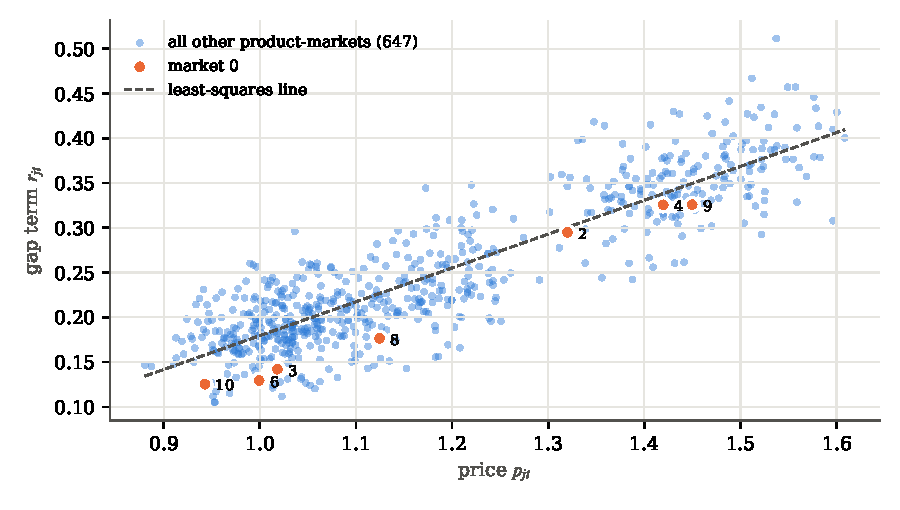
\includegraphics[width=0.85\linewidth]{figures/appC/gap.pdf}
\caption{The gap term $r_{jt} = \ln\frac{s_{jt}}{s_{0t}} - \delta_{jt}$ against price for all 654 observations, with market 0
highlighted and its products labelled. $\delta_{jt}$ is the random coefficients mean utility recovered with the true
$\Sigma$. The correlation with price is 0.888. The dashed simple least-squares line has slope 0.378. The 2SLS price
coefficient, which controls for characteristics, is 0.284.}
\label{fig:C-gap}
\end{figure}

The estimated bias $\hat b_{r,p} = 0.284$ is about 0.7 standard errors of $\hat\alpha^l$, so a single sample cannot
detect it. It comes from one sample of 654 observations, with 1,000 simulation draws per market, so it contains
sampling and simulation error. Its population counterpart $b_{r,p}$ is the probability limit of the bias
(\cref{prop:C-logit-bias}). Unlike sampling error, $b_{r,p}$ does not shrink as the number of markets grows. The
consequences of the bias also propagate. A price coefficient that is too small makes demand look too inelastic,
which inflates the logit markups $\frac{1}{\alpha^l(1 - S_{ft})}$ to a mean of 0.396 against the true 0.386. Better instruments cannot repair it, because the problem lies in the functional form.
The remedy is to model the heterogeneity, which \cref{sec:C-rc-est} does. \Cref{sec:08-worked} reports the same comparison
within the full estimation of the random coefficients model.

\subsection{Computational notes}

\begin{enumerate}
  \item Build the instruments with group sums: within each market and owner, sum each characteristic and subtract the
  product's own value for the firm's other products. The market sum minus the firm sum gives the rival products.
  \item Compute 2SLS through the projected regressors $\hat X$. Code the clustered sandwich by hand and check it against
  a packaged routine. Here the coefficients and standard errors agree to within $2\times10^{-12}$.
  \item For Hansen's $J$, run 2SLS, form $\hat S = \frac{1}{N}\sum_t(Z_t^\top\hat e_t)(Z_t^\top\hat e_t)^\top$ from its
  residuals, re-estimate with weight $\hat S^{-1}$, and compute $J = N\bar g^\top\hat S^{-1}\bar g$ at the second-step
  estimate.
  \item For the bootstrap, note that $mc_{jt}(\alpha) = p_{jt} - \frac{k_{jt}}{\alpha}$ with $k_{jt}$ fixed by the data,
  so each replication needs only one 2SLS fit and one OLS fit.
  \item For joint GMM, concentrate out the linear parameters for each $\alpha^l$ by weighted least squares, minimize the
  concentrated objective over a grid and refine with a bounded scalar search.
  \item For the gap term, run the contraction from the logit start $\ln\frac{s_{jt}}{s_{0t}}$ with draws held fixed, and
  evaluate shares with the overflow-safe routine of \cref{sec:C-simulate}.
\end{enumerate}
The bootstrap loop is short.
\begin{verbatim}
rng = np.random.default_rng(2031)
for b in range(5000):
    pick = rng.integers(0, 100, size=100)            # markets
    rows = np.concatenate([idx[m] for m in pick])
    xh = Z[rows] @ np.linalg.lstsq(Z[rows], X[rows], rcond=None)[0]
    coef = np.linalg.lstsq(xh, y[rows], rcond=None)[0]   # 2SLS
    mc = p - k / (-coef[3])                          # new alpha
    gam = np.linalg.lstsq(W[rows], mc[rows], rcond=None)[0]
    draws[b] = np.append(coef, gam)
\end{verbatim}

\section{Random coefficients estimation and a comparison of the three models}\label{sec:C-rc-est}

Sections \ref{sec:C-vertical} and \ref{sec:C-logit-est} estimated two misspecified models on the simulated market of
\cref{sec:C-simulate}. The vertical model allowed one dimension of taste, and the logit allowed none beyond the
idiosyncratic shock. In this problem we estimate the model that generated the data. We take the dispersion of tastes
$\Sigma$ as known. This isolates the two steps on which random coefficients estimation rests. The first is the
inversion of market shares by the contraction of \citet{BerryLevinsohnPakes1995}. The second is linear instrumental
variables on the recovered mean utilities. With the true structure in hand we then compare the three models on elasticities, diversion, markups,
recovered costs and the predicted effects of a merger. \Cref{sec:08-worked} estimates $\Sigma$ itself on the same data.

\subsection{Statement}

Use the data of \cref{sec:C-simulate} and \cref{ass:C-est}. In each of the 100 markets the econometrician observes
prices, realized shares $s^{obs}_{jt}$, characteristics $x_{jt}$, the milk price $w_{jt}$, the owners and the market
size. The realized shares are the shares $\hat s_{jt}$ of \eqref{eq:C-realized}. Demand is the random coefficients logit
\eqref{eq:C-rc-utility},
\begin{equation}\label{eq:C-rc-model}
  u_{ijt} = \delta_{jt} + \mu_{ijt} + \epsilon_{ijt}, \qquad \mu_{ijt} = \tilde x_{jt}\Sigma\nu_i, \qquad
  \delta_{jt} = x_{jt}\beta - \alpha p_{jt} + \xi_{jt},
\end{equation}
with $\tilde x_{jt} = (x_{jt}, p_{jt})$, $\nu_i \sim N(0, I_4)$, independent type-I extreme value shocks
$\epsilon_{ijt}$, and $u_{i0t} = \epsilon_{i0t}$. The term $\mu_{ijt}$ is the consumer-specific deviation from the mean
utility $\delta_{jt}$. The scale matrix $\Sigma = \diag(0.5, 0.2, 0.3, 0.5)$ is known, with $\Sigma_{pp} = 0.5$ its
price entry. The linear parameters $\theta_1 = (\beta, \alpha)$ are unknown. Firms A to D own the products listed in
\cref{tab:C-products} and set prices in a multi-product Bertrand-Nash equilibrium.

\begin{enumerate}[label=(\alph*)]
  \item Draw $n_s = 1{,}000$ vectors $\nu_{it}$ for each market and keep them fixed for the rest of the problem. Why
  must the draws stay fixed?
  \item Write the simulated share function $s_t(\delta_t, \Sigma)$ for a given $\Sigma$ and derive its derivatives
  with respect to $\delta_t$.
  \item Starting from the logit inversion, recover $\delta_t$ in every market with the iteration
  $\delta^{(h+1)}_t = \delta^{(h)}_t + \ln s^{obs}_t - \ln s_t(\delta^{(h)}_t, \Sigma)$. Prove that it converges. Report
  $\delta_t$ for market 0, explain why every mean utility falls relative to the logit start, and account for the gaps
  between the recovered and the true mean utilities.
  \item Estimate $(\beta, \alpha)$ from the recovered mean utilities. Give the identification argument and standard
  errors.
  \item Compute the elasticity matrix of market 0 with the estimation draws, including the outside good. Compare it
  with the true matrix and with the vertical and logit matrices of Sections \ref{sec:C-vertical} and
  \ref{sec:C-logit-est}. Compute the diversion from each product to the outside good. Recover marginal costs under the
  estimated model and compare the three models.
  \item Firms B and C merge. Predict the new equilibrium of market 0 with the logit, the estimated random coefficients
  model and the true model.
  \item How would you proceed if $\Sigma$ were unknown?
\end{enumerate}

\subsection{Solution}

\casehead{Part (a)}
For each market $t$ we draw $n_s = 1{,}000$ vectors $\nu_{it} \sim N(0, I_4)$, $i = 1, \dots, n_s$, once and store
them. The draws use their own seed (2030), different from the seed of the firms' 100 draws in \cref{sec:C-simulate}.
The econometrician does not know which consumer types the firms had in mind. Draws are independent across
markets. The draws stay fixed for three reasons.
\begin{enumerate}
  \item With fixed draws, the simulated share function of part (b) is a deterministic and smooth function of
  $\delta_t$, and the iteration of part (c) has a well-defined fixed point. With fresh draws at every step, the map
  itself would change from one iteration to the next. The iterates would then wander around the solution by the size
  of the simulation error, which part (c) puts at a few hundredths. A stopping rule with tolerance $10^{-10}$ would
  never be met.
  \item When $\Sigma$ is estimated (part (g)), the GMM objective must be a deterministic function of $\Sigma$.
  Otherwise the optimizer compares objective values computed with different draws, and its minimizer is not defined.
  With fixed draws the objective is a smooth function of $\Sigma$, and the simulation asymptotics of
  \citet{PakesPollard1989} can be applied. Because the simulated shares enter the moments through the nonlinear
  inversion, simulation error also adds a bias of order $\frac{1}{n_s}$ (\cref{prop:08-simbias}). Consistency
  therefore requires the number of draws to grow with the sample. With many draws, the simulation error adds a term
  to the variance \citep{BerryLevinsohnPakes1995}.
  \item Fixed draws make the estimator a function of the data and the draws. Its simulation error can then be measured
  by solving again with other draws, as we do in part (c).
\end{enumerate}

\casehead{Part (b)}
Given the draws and a candidate vector of mean utilities $\delta_t = (\delta_{jt})_{j \in \mathcal{J}_t}$, the
individual choice probabilities are
\begin{equation}\label{eq:C-rc-sij-delta}
  s_{ijt}(\delta_t) = \frac{e^{\delta_{jt} + \mu_{ijt}}}{1 + \sum_{k \in \mathcal{J}_t}e^{\delta_{kt} + \mu_{ikt}}} ,
  \qquad
  s_{i0t}(\delta_t) = \frac{1}{1 + \sum_{k \in \mathcal{J}_t}e^{\delta_{kt} + \mu_{ikt}}} ,
\end{equation}
with $\mu_{ijt} = \tilde x_{jt}\Sigma\nu_{it}$, and the simulated shares are
\begin{equation}\label{eq:C-rc-sdelta}
  s_{jt}(\delta_t, \Sigma) = \frac{1}{n_s}\sum_{i=1}^{n_s}s_{ijt}(\delta_t) .
\end{equation}
This is the simulator \eqref{eq:C-rc-simshare} with $\delta_t$ as its argument. Prices enter only through
$\mu_{ijt}$, and they stay at their observed values throughout the inversion. We evaluate \eqref{eq:C-rc-sij-delta}
with the overflow-safe rule of \cref{sec:C-simulate}, part (b). The convergence argument of part (c) rests on the
derivatives of this function.

\begin{lemma}[Derivatives of the simulated shares]\label{lem:C-sdelta}
For every market and every $\delta_t$:
\begin{enumerate}[label=(\roman*)]
  \item $\frac{\partial s_{jt}}{\partial\delta_{kt}} = \frac{1}{n_s}\sum_{i=1}^{n_s}s_{ijt}\big(\indic\{j = k\} -
  s_{ikt}\big)$.
  \item $0 < \frac{\partial s_{jt}}{\partial\delta_{jt}} < s_{jt}$, and $\frac{\partial s_{jt}}{\partial\delta_{kt}} <
  0$ for $k \ne j$.
  \item $\sum_{k \in \mathcal{J}_t}\frac{\partial s_{jt}}{\partial\delta_{kt}} = \frac{1}{n_s}\sum_{i=1}^{n_s}s_{ijt}
  s_{i0t} > 0$.
\end{enumerate}
\end{lemma}

\begin{proof}
Fix a draw, drop $t$, and write $V_{ik} = \delta_k + \mu_{ik}$ and $E_i = 1 + \sum_k e^{V_{ik}}$. By the quotient rule,
\[
  \frac{\partial s_{ij}}{\partial V_{ik}}
  = \frac{\indic\{j = k\}e^{V_{ij}}E_i - e^{V_{ij}}e^{V_{ik}}}{E_i^2}
  = s_{ij}\big(\indic\{j = k\} - s_{ik}\big) .
\]
Since $\frac{\partial V_{ik}}{\partial\delta_k} = 1$, averaging over draws gives (i). For (ii), $0 < s_{ij} < 1$
implies $0 < s_{ij}(1 - s_{ij}) < s_{ij}$ and $-s_{ij}s_{ik} < 0$. For (iii),
$\sum_k s_{ij}(\indic\{j = k\} - s_{ik}) = s_{ij}(1 - \sum_k s_{ik}) = s_{ij}s_{i0}$.
\end{proof}

\casehead{Part (c)}
For market $t$ define the map
\begin{equation}\label{eq:C-blp-map}
  f_t(\delta_t) = \delta_t + \ln s^{obs}_t - \ln s_t(\delta_t, \Sigma) ,
\end{equation}
with logarithms taken element by element. A vector $\delta_t$ is a fixed point of $f_t$ if and only if
$s_t(\delta_t, \Sigma) = s^{obs}_t$, so the fixed points are exactly the mean utilities that rationalize the observed
shares. The iteration $\delta^{(h+1)}_t = f_t(\delta^{(h)}_t)$ is the contraction of
\citet[eq.~6.8]{BerryLevinsohnPakes1995}, written as eq.~(12) of \citet[p.~533]{Nevo2000a}. Each step raises
$\delta_{jt}$ when the model under-predicts the share of product $j$ and lowers it otherwise.

\begin{proposition}[Convergence of the share inversion]\label{prop:C-blp-contraction}
For every market $t$ and every $\delta_t$,
\begin{equation}\label{eq:C-blp-derivs}
  \frac{\partial f_{jt}}{\partial\delta_{kt}} \ge 0 \ \text{ for all } j, k , \qquad
  \eta_{jt}(\delta_t) \equiv \sum_{k \in \mathcal{J}_t}\frac{\partial f_{jt}}{\partial\delta_{kt}}
  = 1 - \frac{\sum_i s_{ijt}s_{i0t}}{\sum_i s_{ijt}} < 1 .
\end{equation}
The equation $s_t(\delta_t, \Sigma) = s^{obs}_t$ therefore has exactly one solution $\delta^*_t$, and the iteration
converges to it from any starting value. If $\eta_{jt} \le \bar\eta < 1$ for every $j$ on a convex set that
contains $\delta^*_t$ and the iterates, then for every $h \ge 0$
\begin{equation}\label{eq:C-blp-rate}
  \big\|\delta^{(h)}_t - \delta^*_t\big\|_\infty \le \bar\eta^{h}\big\|\delta^{(0)}_t - \delta^*_t\big\|_\infty ,
  \qquad
  \big\|\delta^{(h+1)}_t - \delta^{(h)}_t\big\|_\infty \le \bar\eta^{h}\big\|\delta^{(1)}_t - \delta^{(0)}_t\big\|_\infty .
\end{equation}
\end{proposition}

\begin{proof}
Take $F$ in \cref{cor:08-rowsum} to be the distribution that puts mass $\frac{1}{n_s}$ on each draw, so that its
integrals are the averages of \cref{lem:C-sdelta}. The corollary then gives \eqref{eq:C-blp-derivs}, which is
condition (1) of \cref{thm:08-contraction}. This $F$ has finite support,
so the integrability condition of \cref{thm:08-berry94} holds. That theorem then gives the unique solution
$\delta^*_t$.

For the rate, drop $t$, fix $j$ and apply the mean value theorem on the segment between $\delta^*$ and $\delta$:
\[
  f_j(\delta) - f_j(\delta^*) = \sum_k\frac{\partial f_j}{\partial\delta_k}(\tilde\delta)\,(\delta_k - \delta^*_k)
\]
for some $\tilde\delta$ on the segment. The derivatives are nonnegative and sum to at most $\bar\eta$, so
$|f_j(\delta) - \delta^*_j| \le \bar\eta\|\delta - \delta^*\|_\infty$, using $f_j(\delta^*) = \delta^*_j$. Taking the
maximum over $j$ and iterating gives the first inequality in \eqref{eq:C-blp-rate}. The second follows in the same way
from $\delta^{(h+1)} - \delta^{(h)} = f(\delta^{(h)}) - f(\delta^{(h-1)})$.

\Cref{thm:08-berry94} proves convergence for a truncated iteration. The untruncated iteration also converges from any
start. Let $B$ be the sup-norm ball of radius $\|\delta^{(0)} - \delta^*\|_\infty$ around $\delta^*$. It is convex and
compact. The row sums are continuous and below one, so their maximum $\bar\eta$ on $B$ is below one. The bound
$|f_j(\delta) - \delta^*_j| \le \bar\eta\|\delta - \delta^*\|_\infty$ then holds on $B$, so every iterate stays in $B$.
Hence \eqref{eq:C-blp-rate} applies.
\end{proof}

The row sum has a simple meaning. By Bayes' rule over the draws, as in \cref{prop:C-buyer-alpha},
$\frac{\sum_is_{ijt}s_{i0t}}{\sum_is_{ijt}}$ is the probability that a buyer of product $j$ would choose the outside
good in a new choice situation. So $\eta_{jt}$ is one minus the outside-good probability of $j$'s buyers. The
iteration converges fast when the buyers of every product often choose the outside good, which happens when the outside
share is large. It slows down when inside goods dominate the market (\cref{sec:08-inversion}).

We start from the logit inversion $\delta^{(0)}_{jt} = \ln s^{obs}_{jt} - \ln s^{obs}_{0t}$. It is the exact solution
when $\Sigma = 0$, because then every $s_{ijt}$ is the logit probability at $\delta_t$. We stop when
$\|\delta^{(h+1)}_t - \delta^{(h)}_t\|_\infty < 10^{-10}$. The iteration converges in every market, in 11 to 18
iterations (13.9 on average). At the solution the largest gap between log simulated and log observed shares is
$2.5\times10^{-11}$.

Market 0 shows the proposition at work. At the solution the row sums lie between 0.207 and 0.234. The buyers of each
product choose the outside good with probability 0.766 to 0.793, against 0.855 for all simulated consumers. The largest
row sum along the path of the iteration is $\bar\eta = 0.261$. The first step has size 0.280, so by the second
inequality in \eqref{eq:C-blp-rate} the stopping rule must be met by iteration 18. It is met at iteration 15. After the
first step, the ratio of successive step sizes settles at 0.216. This ratio estimates the largest eigenvalue of the
Jacobian of $f_0$ at the solution, which cannot exceed the largest row sum because the Jacobian has nonnegative
entries. Over all 100 markets the largest row sum at the solution is 0.295.

\Cref{tab:C-delta0} reports the mean utilities of market 0. The recovered values are close to the true ones,
$x_{j}\beta - \alpha p_{j0} + \xi_{j0}$, and every one of them lies below its logit start. The next proposition
explains the second fact.

\begin{table}[htbp]
\centering
\caption{Mean utilities in market 0 with $\Sigma$ known}
\label{tab:C-delta0}
\footnotesize
\setlength{\tabcolsep}{4.5pt}
\begin{tabular}{@{}lccccccccc@{}}
\toprule
 & & & Logit start & \multicolumn{2}{c}{Recovered $\hat\delta_j$} & True & \multicolumn{2}{c}{Gap from truth} & S.e.\ of \\
\cmidrule(lr){5-6}\cmidrule(lr){8-9}
Product & Firm & Buyers $q_j$ & $\delta^{(0)}_j$ & 1,000 draws & 100,000 draws & $\delta_j$ & Simulation & Sampling &
$\ln\hat s_j$ \\
\midrule
2 & C & 51 & $-5.110$ & $-5.405$ & $-5.411$ & $-5.581$ & 0.007 & 0.170 & 0.140 \\
3 & C & 249 & $-3.524$ & $-3.666$ & $-3.701$ & $-3.675$ & 0.035 & $-0.026$ & 0.063 \\
4 & B & 124 & $-4.221$ & $-4.547$ & $-4.551$ & $-4.657$ & 0.005 & 0.105 & 0.089 \\
6 & B & 201 & $-3.738$ & $-3.868$ & $-3.905$ & $-3.962$ & 0.037 & 0.058 & 0.070 \\
8 & A & 553 & $-2.726$ & $-2.903$ & $-2.935$ & $-2.941$ & 0.032 & 0.006 & 0.041 \\
9 & D & 57 & $-4.998$ & $-5.324$ & $-5.330$ & $-5.193$ & 0.006 & $-0.137$ & 0.132 \\
10 & C & 199 & $-3.748$ & $-3.874$ & $-3.910$ & $-3.843$ & 0.036 & $-0.067$ & 0.070 \\
\bottomrule
\end{tabular}

\vspace{3pt}
\begin{minipage}{0.97\textwidth}
\footnotesize Notes: $M_0 = 9{,}880$ consumers, outside share 0.8549. The logit start is
$\ln s^{obs}_j - \ln s^{obs}_0$. The recovered values solve $s_t(\delta_t, \Sigma) = s^{obs}_t$ for $t = 0$
with the 1,000 estimation draws (seed 2030) and with 100,000 draws (seed 2032). The simulation gap is the difference between the two
solutions, and the sampling gap is the 100,000-draw solution minus the true value. The last column is
$\sqrt{\frac{1 - s_j}{q_j}}$ from \eqref{eq:C-logshare-var}. Computed with \texttt{figures/appC/src/appC\_rc.py}.
\end{minipage}
\end{table}

\begin{proposition}[Mean utilities below the logit inversion]\label{prop:C-delta-lower}
\begin{enumerate}[label=(\roman*)]
  \item Suppose a market has one inside product with observed share $s^{obs} < \frac{1}{2}$, and the random term
  $\mu_i$ has a nondegenerate distribution that is symmetric about zero. Let $\mathcal{L}(u) = \frac{e^u}{1 + e^u}$ be the logistic distribution function, and let
  $\delta^*$ solve $\E[\mathcal{L}(\delta + \mu_i)] = s^{obs}$. Then
  \[
    \delta^* < \ln\frac{s^{obs}}{1 - s^{obs}} .
  \]
  \item With several inside products, a diagonal $\Sigma$ and $\lVert\Sigma\rVert \to 0$, the gap
  $r_{jt} = \ln\frac{s^{obs}_{jt}}{s^{obs}_{0t}} - \delta^*_{jt}$ is positive up to terms of order $\lVert\Sigma\rVert^3$
  whenever $\|\tilde x_{jt}\Sigma\| > 2\|\bar x_t\Sigma\|$, where $\bar x_t = \sum_k s_{kt}\tilde x_{kt}$ and
  $\|\cdot\|$ is the Euclidean norm.
\end{enumerate}
\end{proposition}

\begin{proof}
(i) Let $\delta_L = \ln\frac{s^{obs}}{1 - s^{obs}}$, the logit inversion, so that $\mathcal{L}(\delta_L) = s^{obs}$ and
$\delta_L < 0$. For $m \ge 0$ define $g(m) = \mathcal{L}(\delta_L + m) + \mathcal{L}(\delta_L - m) - 2\mathcal{L}(\delta_L)$. Then
$g(0) = 0$ and
\[
  g'(m) = \ell(\delta_L + m) - \ell(\delta_L - m) ,
\]
where $\ell(u) = \mathcal{L}(u)(1 - \mathcal{L}(u))$ is the logistic density. It is symmetric about zero and strictly
decreasing in $|u|$. For $m > 0$, $\delta_L < 0$ gives $|\delta_L + m| < |\delta_L| + m = |\delta_L - m|$, so
$g'(m) > 0$ and $g(m) > 0$. By the symmetry of $\mu_i$,
\[
  \E[\mathcal{L}(\delta_L + \mu_i)] = \frac{1}{2}\E\big[\mathcal{L}(\delta_L + \mu_i) + \mathcal{L}(\delta_L - \mu_i)\big]
  = \mathcal{L}(\delta_L) + \frac{1}{2}\E\big[g(|\mu_i|)\big] > s^{obs} ,
\]
with strict inequality because $\mu_i \ne 0$ with positive probability. The function
$\delta \mapsto \E[\mathcal{L}(\delta + \mu_i)]$ is strictly increasing, so its solution $\delta^*$ lies below $\delta_L$.

(ii) By \cref{prop:C-gap-approx}, with $a = \tilde x_{jt}\Sigma$ and $b = \bar x_t\Sigma$ (row vectors, $\Sigma$ diagonal),
$r_{jt} = \frac{1}{2}\|a\|^2 - a b^\top + O(\lVert\Sigma\rVert^3)$. The Cauchy-Schwarz inequality gives $ab^\top \le \|a\|\,\|b\|$,
so $r_{jt} \ge \|a\|\big(\frac{1}{2}\|a\| - \|b\|\big) + O(\lVert\Sigma\rVert^3)$, which is positive when $\|a\| > 2\|b\|$.
\end{proof}

Part (i) is the convexity argument in its cleanest form. The logit probability is convex below one half, so spreading
utility symmetrically around $\delta$ raises the average choice probability. To match the observed share, the mean
utility must fall. Part (ii) covers our design. The vector $\bar x_t$ averages the inside products with weights equal to
their shares, which sum to the inside share of at most 0.21. So $\|\bar x_t\Sigma\|$ is a small fraction of
$\max_k\|\tilde x_{kt}\Sigma\|$, and the condition holds unless products are very different. In the data every one of
the 654 recovered mean utilities lies below its logit start. The gap $r_{jt}$, studied in \cref{sec:C-logit-est},
part (e), has mean 0.247 (\cref{fig:C-gap}). In market 0 it is smallest for product 10, the cheapest, and largest for
products 4 and 9, which are expensive and organic and therefore have the largest $\|\tilde x_{jt}\Sigma\|$.

The gaps from the truth have two sources, which we separate by solving the inversion again with 100,000 draws:
\begin{equation}\label{eq:C-delta-gap}
  \hat\delta_{jt} - \delta_{jt} = \big(\hat\delta_{jt} - \hat\delta^{100k}_{jt}\big) + \big(\hat\delta^{100k}_{jt} -
  \delta_{jt}\big) .
\end{equation}
The first term is simulation error from using 1,000 draws. In market 0 it lies between 0.005 and 0.037. It has the same
sign for every product, which reflects the draws that all products share. It is of the same order as the relative
simulation standard error of the shares, the standard deviation of $s_{ij0}$ across draws divided by
$\sqrt{n_s}\,s_{j0}$, which lies between 0.020 and 0.030. The second term is sampling error. Realized shares are
proportions among about 10,000 consumers, and by \eqref{eq:C-logshare-var} the log share of product $j$ has standard
error near $\sqrt{\frac{1 - s_{j}}{q_{j}}}$. Products 2, 4 and 9 miss the truth by 1.0 to 1.2 of these standard errors,
and the others by less. Both errors are independent across markets. To first order they have mean zero and are uncorrelated with the
instruments, so they act as extra noise in the regression of part (d). The log transformation adds a small
second-order bias that depends on the share, of order $\frac{1}{q_j}$.

\casehead{Part (d)}
With $\Sigma$ known, the recovered mean utilities satisfy the linear equation
\begin{equation}\label{eq:C-rc-linear}
  \hat\delta_{jt} = x_{jt}\beta - \alpha p_{jt} + \xi_{jt} + e_{jt} ,
\end{equation}
where $e_{jt} = \hat\delta_{jt} - \delta_{jt}$ collects the simulation and sampling errors of part (c). Price is
correlated with $\xi_{jt}$ because firms observe $\xi_{jt}$ when they set prices (\cref{sec:C-logit-est}, part (a)).
We therefore estimate \eqref{eq:C-rc-linear} by 2SLS with the instruments of \eqref{eq:C-logit-moments}: the milk price
and the six sums of characteristics and counts of the firm's other products and of rival products. The parameters are
identified by the moment conditions $\E[z_{jt}^\top(\xi_{jt} + e_{jt})] = 0$ and the rank condition of
\cref{sec:C-logit-est}. The error $e_{jt}$ comes from consumers' choices and from the econometrician's draws, given
prices. To first order it has mean zero conditional on $z_{jt}$, so it adds noise without adding bias. The
regressors and instruments are those of the logit, so the first stage is the one in \cref{tab:C-firststage}.

\begin{table}[htbp]
\centering
\caption{Demand estimates with $\Sigma$ known}
\label{tab:C-rc-demand}
\footnotesize
\setlength{\tabcolsep}{4pt}
\begin{tabular}{@{}lccccc@{}}
\toprule
 & Logit & \multicolumn{3}{c}{Random coefficients, $\Sigma$ known} & \\
\cmidrule(lr){2-2}\cmidrule(lr){3-5}
 & 2SLS & OLS & 2SLS & \makecell{2SLS, milk\\price only} & True \\
\midrule
Constant & $-1.184$ (0.329) & $-1.355$ (0.227) & $-1.061$ (0.330) & $-1.042$ (0.335) & $-1.00$ \\
Sugar content & 0.190 (0.158) & 0.088 (0.122) & 0.168 (0.158) & 0.173 (0.156) & 0.20 \\
Organic & 0.153 (0.141) & $-0.002$ (0.097) & 0.114 (0.142) & 0.121 (0.143) & 0.15 \\
Price coefficient $\alpha$ & 2.641 (0.412) & 2.573 (0.252) & 2.926 (0.413) & 2.948 (0.415) & 3.00 \\
\midrule
First-stage $F$ & 92.5 & & 92.5 & & \\
Hansen $J$ (df, $p$) & 8.82 (6, 0.18) & & 8.16 (6, 0.23) & & \\
Observations & 654 & 654 & 654 & 654 & \\
\bottomrule
\end{tabular}

\vspace{3pt}
\begin{minipage}{0.97\textwidth}
\footnotesize Notes: The dependent variable is $\ln s^{obs}_{jt} - \ln s^{obs}_{0t}$ for the logit and the recovered
$\hat\delta_{jt}$ otherwise. Standard errors in parentheses are clustered by market with the factor
$\frac{G}{G - 1}\frac{N - 1}{N - K}$ and condition on $\Sigma$. The first and third 2SLS columns use the milk price and
the six competition instruments, and the last uses the milk price alone. The logit column repeats \cref{tab:C-logit-demand}. Computed with
\texttt{figures/appC/src/appC\_rc.py}.
\end{minipage}
\end{table}

\Cref{tab:C-rc-demand} reports the estimates. The 2SLS estimate of the price coefficient is 2.926, within 0.18
standard errors of the true value of 3. OLS gives 2.573, biased toward zero for the same reason as in the logit. Using
the milk price alone gives 2.948 with a slightly larger standard error, so the six competition instruments add little,
as in \cref{sec:C-logit-est}. Hansen's test does not reject the overidentifying restrictions ($J = 8.16$, $p = 0.23$).
The coefficients on sugar and organic production are close to the truth but imprecise. They are identified from ten
products whose characteristics never change, so the data contain only ten distinct combinations of characteristics.

The comparison with the logit is exact. By \cref{prop:C-logit-bias}, the logit estimate equals the random coefficients
estimate minus the 2SLS price coefficient of the gap term $r_{jt}$ on the same regressors and instruments. That
coefficient is 0.284, and the identity $2.641 = 2.926 - 0.284$ holds to machine precision (\cref{sec:C-logit-est},
part (e)). Allowing for the random coefficients
moves the estimate from 0.359 below the truth to 0.074 below it. The remaining gap is well within sampling error. The
estimates also imply sensible individual tastes. Across the 100,000 estimation draws, the smallest price sensitivity
$\alpha_i = \hat\alpha - \Sigma_{pp}\nu_{i4}$ is 0.814, so every simulated consumer dislikes higher prices, as
\cref{prop:C-ms} requires.

The standard errors cluster by market, with the sandwich \eqref{eq:C-clustervar}. The recovered $\hat\delta_t$ depends
only on the shares and draws of market $t$, so the errors are independent across markets and clustering is valid. The
standard errors condition on $\Sigma$. If $\Sigma$ were estimated, $\hat\theta_1 = \hat\theta_1(\hat\Sigma)$ would inherit
the uncertainty in $\hat\Sigma$, and all parameters would be estimated jointly as in part (g).

\casehead{Part (e)}
A change in $p_{kt}$ moves both the mean utility, through $-\alpha$, and the random term, through $\Sigma_{pp}\nu_{i4}$.
For draw $i$ the price coefficient is therefore $-\alpha_i$ with $\alpha_i = \hat\alpha - \Sigma_{pp}\nu_{i4}$. Applying
\cref{lem:C-sdelta}(i) draw by draw, with $\frac{\partial V_{ikt}}{\partial p_{kt}} = -\alpha_i$, gives the share
derivatives
\begin{equation}\label{eq:C-rc-elast}
  \frac{\partial s_{jt}}{\partial p_{kt}} = \frac{1}{n_s}\sum_{i=1}^{n_s}\alpha_is_{ijt}\big(s_{ikt} - \indic\{j = k\}\big) ,
  \qquad
  \frac{\partial s_{0t}}{\partial p_{kt}} = \frac{1}{n_s}\sum_{i=1}^{n_s}\alpha_is_{i0t}s_{ikt} .
\end{equation}
The second formula follows from $\frac{\partial s_{i0t}}{\partial V_{ikt}} = -s_{i0t}s_{ikt}$. The elasticities are
$\varepsilon_{jk} = \frac{\partial s_j}{\partial p_k}\frac{p_k}{s_j}$ and
$\varepsilon_{0k} = \frac{\partial s_0}{\partial p_k}\frac{p_k}{s_0}$. Own entries are negative, so the positive own
elasticity of the book's notation is $-\varepsilon_{jj}$. The estimated matrix uses $\hat\alpha = 2.926$, the recovered
$\hat\delta_0$ and the 1,000 estimation draws. The true matrix uses the true parameters, the true mean utilities and
the firms' 100 draws, the demand system that generated the prices. \Cref{tab:C-rcelast} reports both.

\begin{table}[htbp]
\centering
\caption{Random coefficients elasticities in market 0}
\label{tab:C-rcelast}
\footnotesize
\begin{tabular}{@{}lrrrrrrr@{}}
\toprule
 & \multicolumn{7}{c}{Price of product} \\
\cmidrule(lr){2-8}
Share of & 2 & 3 & 4 & 6 & 8 & 9 & 10 \\
\midrule
\multicolumn{8}{@{}l}{\emph{Panel A. Estimated model ($\hat\alpha = 2.926$, $\Sigma$ known)}} \\
Product 2 & $-3.45$ & 0.10 & 0.08 & 0.07 & 0.24 & 0.04 & 0.07 \\
Product 3 & 0.03 & $-2.68$ & 0.07 & 0.07 & 0.23 & 0.03 & 0.07 \\
Product 4 & 0.03 & 0.10 & $-3.63$ & 0.08 & 0.24 & 0.04 & 0.07 \\
Product 6 & 0.02 & 0.09 & 0.07 & $-2.65$ & 0.23 & 0.03 & 0.07 \\
Product 8 & 0.03 & 0.09 & 0.07 & 0.07 & $-2.79$ & 0.03 & 0.07 \\
Product 9 & 0.03 & 0.10 & 0.08 & 0.08 & 0.24 & $-3.74$ & 0.07 \\
Product 10 & 0.02 & 0.09 & 0.07 & 0.07 & 0.23 & 0.03 & $-2.51$ \\
Outside good & 0.02 & 0.07 & 0.04 & 0.05 & 0.16 & 0.02 & 0.05 \\
\midrule
\multicolumn{8}{@{}l}{\emph{Panel B. True model}} \\
Product 2 & $-3.57$ & 0.12 & 0.09 & 0.08 & 0.29 & 0.05 & 0.09 \\
Product 3 & 0.03 & $-2.74$ & 0.07 & 0.08 & 0.26 & 0.04 & 0.08 \\
Product 4 & 0.03 & 0.12 & $-3.74$ & 0.08 & 0.29 & 0.05 & 0.09 \\
Product 6 & 0.03 & 0.10 & 0.07 & $-2.71$ & 0.25 & 0.04 & 0.08 \\
Product 8 & 0.03 & 0.11 & 0.08 & 0.08 & $-2.84$ & 0.05 & 0.08 \\
Product 9 & 0.03 & 0.12 & 0.09 & 0.08 & 0.29 & $-3.85$ & 0.09 \\
Product 10 & 0.03 & 0.10 & 0.07 & 0.07 & 0.26 & 0.04 & $-2.57$ \\
Outside good & 0.02 & 0.07 & 0.04 & 0.05 & 0.17 & 0.03 & 0.06 \\
\bottomrule
\end{tabular}

\vspace{3pt}
\begin{minipage}{0.97\textwidth}
\footnotesize Notes: Entry $(j, k)$ is $\varepsilon_{jk} = \frac{\partial s_j}{\partial p_k}\frac{p_k}{s_j}$, the
percentage change in the share of the row alternative after a one percent rise in the price of the column product.
Panel A uses the 1,000 estimation draws and the recovered mean utilities. Panel B uses the true parameters and mean
utilities and the firms' 100 draws. Computed with \texttt{figures/appC/src/appC\_rc.py}.
\end{minipage}
\end{table}

The estimated matrix is close to the true one. The largest absolute difference between corresponding entries is 0.11.
The estimated own elasticities run from $-2.51$ to $-3.74$, against $-2.57$ to $-3.85$ in the truth. They are slightly
smaller in magnitude because $\hat\alpha$ is slightly below 3. Three features distinguish the random coefficients
matrix from the other two models.

First, cross elasticities differ within a column. In the logit every off-diagonal entry of column $k$ equals
$\hat\alpha^lp_ks_k$ (\cref{tab:C-lelast}). In Panel A the largest ratio between two cross elasticities in the same
column is 1.21, and in the truth it is 1.27. The pattern has an economic logic. A rise in the price of product 4 raises
the shares of products 2 and 9 by more than those of the other products. The same holds for the columns of products 2
and 9. The three products are the organic ones and also the most expensive. Their buyers have high draws of the
organic taste $\nu_{i3}$ or low price sensitivity $\alpha_i$. When they leave one of these products, they look for
another product that suits the same tastes.

Second, the outside good receives less substitution than the logit implies. The diversion ratio from product $k$ to
the outside good (\cref{sec:C-logit-bertrand}, part (e), and \cref{sec:C-vertical}, part (e)) is
\begin{equation}\label{eq:C-div0}
  D_{k0} = \frac{\frac{\partial s_0}{\partial p_k}}{-\frac{\partial s_k}{\partial p_k}}
  = \frac{\sum_i\alpha_is_{ik}s_{i0}}{\sum_i\alpha_is_{ik}(1 - s_{ik})}
  = \sum_i\varpi_{ik}\frac{s_{i0}}{1 - s_{ik}} , \qquad
  \varpi_{ik} = \frac{\alpha_is_{ik}(1 - s_{ik})}{\sum_l\alpha_ls_{lk}(1 - s_{lk})} .
\end{equation}
The second equality uses \eqref{eq:C-rc-elast}. The third writes $D_{k0}$ as a weighted average of the individual logit
diversion ratios $\frac{s_{i0}}{1 - s_{ik}}$, with weights that favour the draws most likely to buy $k$. In the logit
all draws are alike and $D_{k0} = \frac{s_0}{1 - s_k}$, which lies between 85.9 and 90.6 percent in market 0. Under the
estimated random coefficients model it lies between 79.2 and 86.7 percent, and in the truth between 76.2 and 85.1
percent. The buyers of a product are disproportionately consumers with a high draw of the random constant. Their
probability of choosing the outside good is 0.77 to 0.79, against 0.855 on average, so they divert less of their
purchases to it. The logit cannot represent this selection. It overstates diversion to the outside good by 5 to 10
percentage points relative to the truth and understates diversion among inside goods, which matters for the merger of part (f).

Third, the vertical model is far from both (\cref{tab:C-velast}). Its own elasticities range from $-16.8$ to
$-358.4$. Their mean absolute value, 126.6, is 41 times that of the logit. Each row has at most two nonzero cross elasticities, one for each
neighbour on the price ladder. Only the cheapest product, product 10, loses sales to the outside good, and only 6.4
percent of them. \Cref{fig:C-own-elas} summarizes the own elasticities. \Cref{fig:08-ownelas} shows the logit and random
coefficients panels on the same data.

\begin{figure}[htbp]
\centering
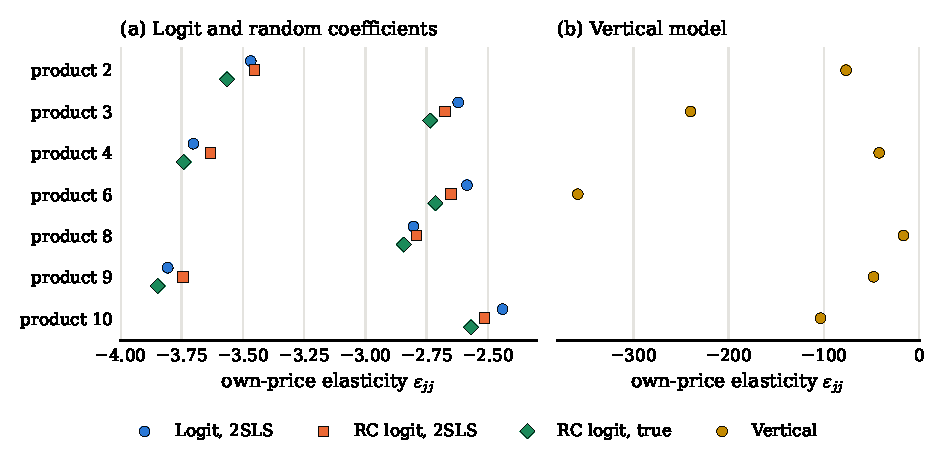
\includegraphics[width=\linewidth]{figures/appC/own_elas.pdf}
\caption{Own-price elasticities in market 0 by product. Panel (a): logit estimated by 2SLS, random coefficients logit
estimated by 2SLS with $\Sigma$ known, and the true random coefficients model. Panel (b): the vertical model, on its own
scale. Computed with \texttt{figures/appC/src/appC\_rc.py}.}
\label{fig:C-own-elas}
\end{figure}

We now recover marginal costs. Under the estimated model, the stacked first-order conditions
\eqref{eq:C-stacked-foc} give
\begin{equation}\label{eq:C-rc-mc-hat}
  \widehat{mc}_t = p_t + \big(\Omega_t \odot \hat\Delta_t^\top\big)^{-1}s^{obs}_t ,
\end{equation}
with $\hat\Delta_t$ the matrix of share derivatives \eqref{eq:C-rc-elast}. We regress $\widehat{mc}_{jt}$ on
$(x_{jt}, w_{jt})$ by OLS. The regressand depends on $\hat\alpha$, so we compute standard errors with a bootstrap over
markets (5,000 resamples, seed 2031) that re-estimates $\hat\alpha$ in each replication. With $\Sigma$ known,
$\hat\delta_t$ does not depend on $\alpha$, so only $\hat\Delta_t$ changes across replications. \Cref{tab:C-compare}
collects the comparison.

\begin{table}[htbp]
\centering
\caption{Three demand models estimated on the same simulated data}
\label{tab:C-compare}
\footnotesize
\setlength{\tabcolsep}{4pt}
\begin{tabular}{@{}lcccc@{}}
\toprule
 & Vertical & Logit & \makecell{Random coefficients\\($\Sigma$ known)} & True \\
\midrule
Price coefficient $\alpha$ & none & 2.641 (0.412) & 2.926 (0.413) & 3.00 \\
Own elasticities, market 0 & $-16.8$ to $-358.4$ & $-2.44$ to $-3.81$ & $-2.51$ to $-3.74$ & $-2.57$ to $-3.85$ \\
Nonzero cross elasticities per row & 1 or 2 & 6 & 6 & 6 \\
Largest ratio within a column & & 1.00 & 1.21 & 1.27 \\
Diversion to outside good, market 0 (\%) & 0 to 6.4 & 85.9 to 90.6 & 79.2 to 86.7 & 76.2 to 85.1 \\
\midrule
Mean markup, all observations & 0.048 & 0.396 & 0.397 & 0.386 \\
Range of markups & 0.000 to 0.515 & 0.379 to 0.426 & 0.368 to 0.452 & 0.348 to 0.451 \\
Correlation with true markups & 0.275 & 0.553 & 0.715 & 1 \\
Mean absolute markup error & 0.340 & 0.014 & 0.013 & 0 \\
\midrule
\multicolumn{5}{@{}l}{\emph{Marginal cost equation}} \\
Constant & 0.674 (0.024) & 0.160 (0.072) & 0.188 (0.060) & 0.20 \\
Sugar content & 0.194 (0.014) & 0.258 (0.010) & 0.246 (0.010) & 0.25 \\
Organic & 0.271 (0.009) & 0.315 (0.006) & 0.305 (0.006) & 0.30 \\
Price of milk & 0.356 (0.031) & 0.532 (0.023) & 0.504 (0.026) & 0.50 \\
\bottomrule
\end{tabular}

\vspace{3pt}
\begin{minipage}{0.97\textwidth}
\footnotesize Notes: All models assume multi-product Bertrand-Nash pricing. Cross elasticities and diversion refer to
market 0. Markup statistics use all 654 observations. Cost equations are OLS regressions of the implied marginal cost
on the characteristics and the milk price. Standard errors are clustered by market for the vertical model, whose markups
contain no estimated parameter. For the logit and the random coefficients model they come from a market bootstrap
that re-estimates $\alpha$ (5,000 replications). Computed with \texttt{figures/appC/src/appC\_rc.py}.
\end{minipage}
\end{table}

The random coefficients model wins on every dimension that depends on substitution. Its cost coefficients are the
closest to the truth, and its implied markups track the true markups across observations more closely (correlation
0.715, against 0.553 for the logit). The mean markups of the logit and the random coefficients model are almost equal.
Both are near $\frac{1}{\hat\alpha}$ corrected for the firm's share, and both overstate the true mean of 0.386 a little
because both price coefficients lie below 3. The vertical model fails on every dimension, for the reasons of
\cref{sec:C-vertical}. Adjacent prices are close, its elasticities explode, and its markups collapse toward zero, so
its cost intercept absorbs the true markup.

\casehead{Part (f)}
Firms B and C merge. In market 0, firm B sells products 4 and 6 and firm C sells products 2, 3 and 10. After the merger
one firm owns all five, while firm A (product 8) and firm D (product 9) are unchanged. We predict the new equilibrium
under three demand models: the logit of \cref{sec:C-logit-est}, the estimated random coefficients model of parts (c) and
(d), and the true model. The procedure is the same for each.
\begin{enumerate}
  \item Recover marginal costs from the pre-merger first-order conditions of the model, \eqref{eq:C-rc-mc-hat} or its
  logit version. For the true model use the true marginal costs. Each model then reproduces the observed prices.
  Solving the pre-merger game again returns them to within $3\times10^{-14}$.
  \item Hold marginal costs, unobserved qualities and draws fixed. As prices move, mean utilities move as
  $\delta_{jt}(p) = \hat\delta_{jt} - \alpha(p_{jt} - p^{obs}_{jt})$, and $\mu_{ijt}$ moves through the price entry of
  $\tilde x_{jt}$.
  \item Replace $\Omega_0$ by the post-merger ownership matrix and solve the first-order conditions. For the logit
  iterate $p \leftarrow mc + \frac{1}{\alpha(1 - S_f(p))}$, using \cref{prop:C-common-markup}. For the random
  coefficients models iterate the Morrow-Skerlos map \eqref{eq:C-ms-zeta}. Each converges in 11 iterations to a tolerance
  of $10^{-12}$, and 20 random starting points lead to the same prices to within $9\times10^{-14}$.
  \item Measure consumer welfare by the log-sum formula (\cref{prop:07-logsum}). A consumer with marginal utility of
  income $\alpha_i$ has expected surplus $\frac{1}{\alpha_i}\ln\big(1 + \sum_je^{V_{ij}}\big)$ up to a constant, and we
  average over draws. The constant cancels from the change.
\end{enumerate}

\begin{table}[htbp]
\centering
\caption{Merger of firms B and C in market 0}
\label{tab:C-merger-m0}
\footnotesize
\setlength{\tabcolsep}{4pt}
\begin{tabular}{@{}lcccccccc@{}}
\toprule
 & & & \multicolumn{3}{c}{Equilibrium price change} & \multicolumn{3}{c}{Upward pricing pressure} \\
\cmidrule(lr){4-6}\cmidrule(lr){7-9}
Product & Firm & Price & Logit & RC est. & RC true & Logit & RC est. & RC true \\
\midrule
2 & C & 1.3200 & 0.0129 & 0.0207 & 0.0220 & 0.0129 & 0.0194 & 0.0204 \\
3 & C & 1.0182 & 0.0129 & 0.0184 & 0.0188 & 0.0132 & 0.0178 & 0.0181 \\
4 & B & 1.4196 & 0.0202 & 0.0309 & 0.0356 & 0.0204 & 0.0296 & 0.0340 \\
6 & B & 0.9993 & 0.0202 & 0.0277 & 0.0305 & 0.0206 & 0.0268 & 0.0294 \\
8 & A & 1.1246 & 0.0001 & 0.0004 & 0.0006 & & & \\
9 & D & 1.4497 & 0.0000 & 0.0002 & 0.0002 & & & \\
10 & C & 0.9429 & 0.0129 & 0.0181 & 0.0185 & 0.0131 & 0.0174 & 0.0177 \\
\midrule
Mean change, merging & & & 0.0158 & 0.0231 & 0.0251 & & & \\
Outside share, before, after & & & \makecell{0.8549\\0.8578} & \makecell{0.8549\\0.8589} &
\makecell{0.8463\\0.8507} & & & \\
Change in consumer surplus & & & $-12.78$ & $-18.37$ & $-20.39$ & & & \\
Change in merged profit & & & 0.28 & 0.58 & 0.72 & & & \\
Change in rivals' profit & & & 0.83 & 1.68 & 2.13 & & & \\
Change in total surplus & & & $-11.67$ & $-16.11$ & $-17.54$ & & & \\
\bottomrule
\end{tabular}

\vspace{3pt}
\begin{minipage}{0.97\textwidth}
\footnotesize Notes: Firm B owns products 4 and 6 and firm C owns products 2, 3 and 10 in market 0. Upward pricing
pressure is $\sum_kD_{jk}(p_k - mc_k)$ over the partner firm's products, evaluated before the merger. Surplus and profit
changes are totals over the $M_0 = 9{,}880$ consumers, in the same money units as prices. The true model's outside
share differs before the merger because it uses expected rather than realized shares. Computed with
\texttt{figures/appC/src/appC\_rc\_merger.py}.
\end{minipage}
\end{table}

\Cref{tab:C-merger-m0} reports the predictions. Under the logit, the price increase is the same for every product of a
merging firm, 0.0129 for firm C and 0.0202 for firm B. \Cref{prop:C-common-markup} explains it. Logit
markups are common within a firm, so after the merger the new firm sets one markup $\frac{1}{\alpha(1 - S_{BC})}$ on
all five products. That markup is 0.4117, up from 0.3988 for firm C and 0.3915 for firm B. Firm B's products start from
the lower markup, so they rise more. Under the random coefficients models the increases differ across products and are
largest for products 4 and 6.

The logit understates the merger's effect. The mean increase on the merging products is 0.0158 under the logit, 0.0231
under the estimated random coefficients model and 0.0251 in the truth. The logit captures 63 percent of the true effect
and the estimated model 92 percent. In percentage terms the true increases range from 1.7 to 3.1 percent. The source is
diversion between the merging firms. Consider the share of a merging product's lost sales that goes to the partner firm.
It is 0.033 to 0.052 under the logit, 0.044 to 0.075 under the estimated model and 0.046 to 0.088 in the truth. The logit sends too
many lost sales to the outside good, as part (e) showed, so it sees the two firms as weaker competitors than they are.

First-order upward pricing pressure, defined in \cref{sec:C-logit-bertrand}, part (g), is the opportunity cost
$\sum_kD_{jk}(p_k - mc_k)$ of sales diverted to the partner \citep{FarrellShapiro2010}, discussed in \cref{sec:11-upp}.
It is close to the equilibrium price change in all three models.
For product 4 in the truth, for example, it is 0.0340 against an equilibrium increase of 0.0356. Inside shares are
small, so pass-through is close to one and the feedback among prices is weak. Rivals raise their prices only slightly,
by at most 0.0006, because prices are strategic complements. Consumer surplus falls by 20.39 in the truth, while the
merged firm gains 0.72 and its rivals 2.13. Without cost savings the merger lowers total surplus. The logit predicts
a loss of 11.67, about two thirds of the true loss of 17.54.

The two estimated models agree here more than they would in many markets. Inside shares are small and the products are
similar, so all predicted increases are below 4 percent. The gap
between the logit and the random coefficients model would widen with larger inside shares or more dispersed tastes. It
would also widen if the merging products were closer in characteristics, as in a merger of the owners of the three
organic products.

We do not solve the merger under the vertical model, because its prediction would depend mainly on the price ladder.
In the vertical model every lost sale goes to a neighbour on the price ladder. In market 0 the ladder runs through
products 10, 6, 3, 8, 2, 4 and 9 in increasing order of price. Both neighbours of product 6 belong to firm C, so all of product 6's lost
sales go to the partner. The share is 0.936 for product 10, 0.879 for product 3, 0.605 for product 2 and 0.488 for
product 4. The merger therefore internalizes much of the competition each merging product faces, while the
pre-merger markups that would enter the upward pricing pressure are near zero. A prediction built on these two
artefacts would tell us about the price gaps in market 0 more than about preferences.

\casehead{Part (g)}
When $\Sigma$ is unknown we estimate $\theta = (\theta_1, \theta_2)$, where $\theta_2$ collects the four diagonal
entries of $\Sigma$. The estimator is GMM with the nested fixed point algorithm of \citet{BerryLevinsohnPakes1995}, as
laid out by \citet[Section 3.3]{Nevo2000a}. The steps are as follows.
\begin{enumerate}
  \item Fix the draws, as in part (a).
  \item Inner loop. For a trial $\theta_2$, solve $s_t(\delta_t, \Sigma) = s^{obs}_t$ in every market by the iteration
  of part (c), starting from the solution at the previous trial value. Use a tight tolerance, because errors in
  $\delta$ pass into the objective and can stop the outer search at false minima \citep{DubeFoxSu2012}.
  \item Form the structural error $\xi_{jt}(\theta) = \delta_{jt}(\theta_2) - x_{jt}\beta + \alpha p_{jt}$
  \citep[eq.~13, p.~533]{Nevo2000a}.
  \item Concentrate out the linear parameters. With $X$ the matrix of rows $(x_{jt}, -p_{jt})$, the minimizer given
  $\theta_2$ is $\hat\theta_1(\theta_2) = (X^\top Z\mathcal{W}Z^\top X)^{-1}X^\top Z\mathcal{W}Z^\top\delta(\theta_2)$
  (\cref{prop:08-concentrate}).
  \item Outer loop. Minimize $Q(\theta_2) = \xi(\theta_2)^\top Z\mathcal{W}Z^\top\xi(\theta_2)$ \citep[eq.~9]{Nevo2000a} over
  $\theta_2 \ge 0$, which removes the sign indeterminacy of \cref{prop:08-signsigma}. A quasi-Newton method needs the
  derivatives of $\delta$, which the implicit function theorem gives from $s_t(\delta_t(\Sigma), \Sigma) = s^{obs}_t$:
  \begin{equation}\label{eq:C-ddelta-dsigma}
    \frac{\partial\delta_t}{\partial\Sigma_{kk}} = -\Big[\frac{\partial s_t}{\partial\delta_t^\top}\Big]^{-1}
    \frac{\partial s_t}{\partial\Sigma_{kk}} , \qquad
    \frac{\partial s_{jt}}{\partial\Sigma_{kk}} = \frac{1}{n_s}\sum_i s_{ijt}\,\nu_{ikt}\Big(\tilde x_{jtk} -
    \sum_ls_{ilt}\tilde x_{ltk}\Big) .
  \end{equation}
  The second formula follows from $\frac{\partial V_{ijt}}{\partial\Sigma_{kk}} = \tilde x_{jtk}\nu_{ikt}$ and the
  quotient rule, as in \cref{lem:C-sdelta}. The matrix $\frac{\partial s_t}{\partial\delta_t^\top}$ is invertible. By
  \cref{lem:C-sdelta}(ii) and (iii), its diagonal entries are positive, its other entries are negative and its row
  sums are positive, so it is strictly diagonally dominant by rows.
  \item Use a first-step weight such as $(\frac{1}{N}Z^\top Z)^{-1}$, then the inverse of the market-clustered
  covariance of the moments, and restart the search from several points.
  \item Compute standard errors from the GMM sandwich with the Jacobian of the moments with respect to all of
  $\theta$. The covariance of the moments adds a simulation term to the sampling term \citep{BerryLevinsohnPakes1995}.
\end{enumerate}

The instruments need more care than with $\Sigma$ known. The moments must change with $\theta_2$ for $\Sigma$ to be
identified. \citet[p.~529]{Nevo2000a} gives the intuition. Suppose products A and B are similar and B and C have the
same share. A rise in the price of A should then raise the share of B more than that of C. The size of the difference
identifies the dispersion of tastes. The data must therefore contain variation in choice sets and characteristics
across markets. In this design characteristics are fixed by product, so the variation comes from which products each
market offers. Instruments that measure how crowded a product's neighbourhood in characteristics space is
\citep{GandhiHoude2019}, or approximations to the optimal instruments $\E[\frac{\partial\xi_{jt}}{\partial\theta}
\mid z_t]$, put this variation to work. Supply moments can add information (\cref{sec:08-supply-joint}), and the
problem can also be written as a constrained optimization (\cref{sec:08-mpec}). \Cref{sec:08-worked-nfxp} carries out
this estimation on the same data and shows that the instruments decide how precisely $\Sigma$ is estimated.

\subsection{Computational notes}

The script \texttt{appC\_rc.py} in \texttt{figures/appC/src} reads the simulated data in
\texttt{figures/appC/data} and uses only the observables for estimation. It runs in about a minute.
\begin{enumerate}
  \item Build the seven instruments of \cref{sec:C-logit-est} and run the logit regressions.
  \item Draw an array of shape $100 \times 1{,}000 \times 4$ with seed 2030 and save it as
  \texttt{est\_draws.npz} in the data folder.
  \item Invert shares market by market from the logit start. For market 0 also invert with 100,000 draws (seed 2032).
  \item Run 2SLS on $\hat\delta$, compute Hansen's $J$ by two-step GMM, and run 2SLS of $r_{jt}$ to check
  \cref{prop:C-logit-bias}.
  \item Compute the elasticity matrices and the implied marginal costs. Store $\hat\Delta_t = \alpha A_t + B_t$, where
  $A_t$ and $B_t$ do not depend on $\alpha$, so that each bootstrap replication only rescales them.
\end{enumerate}
The script \texttt{appC\_rc\_merger.py} solves the merger, and \texttt{appC\_part4\_tables.py} prints the table rows.
The inner loop is short:
\begin{verbatim}
def invert_shares(s_obs, xtilde, nu, sigma, delta0, tol=1e-10):
    delta, log_s = delta0.copy(), np.log(s_obs)
    while True:
        new = delta + log_s - np.log(shares_delta(delta, xtilde, nu, sigma))
        if np.max(np.abs(new - delta)) < tol:
            return new
        delta = new
\end{verbatim}

\section{Markups over time in the U.S. automobile market}\label{sec:C-autos}

The previous four problems used data whose generating model we knew, so every estimate could be checked against the
truth. This last problem uses real data, where no such check exists and the choice of model must be argued. Did market
power in the U.S. new-car market rise or fall after 1980? Production-function estimates for listed firms
point to rising average markups across the economy \citep{DeLoeckerEeckhoutUnger2020}, a literature reviewed in
\cref{sec:01-rising-markups}. \citet{GriecoMurryYurukoglu2024}, GMY for short, answer the question for one industry
with a demand system and a model of pricing. They find that markups fell substantially while real prices rose (abstract and
Section~5.4). We cite their author manuscript of July 5, 2023, and its table, figure and page numbers may differ from
those of the published article. In this problem we use the product data of their public replication package. We
estimate simple demand models, compute the markups they imply year by year, and ask what kind of decline these models
measure. The answer turns on the functional form of price. Part (e) then compares our results with their full model.

\subsection{Statement}

The data are the product file of the replication package of \citet{GriecoMurryYurukoglu2024}, deposited on the Harvard
Dataverse (doi:10.7910/DVN/CZGOKP). An observation is a vehicle model in a year. There are 9,694 model-years in 39
annual markets from 1980 to 2018, 1,067 distinct models, and between 165 and 323 models per year. Models belong to 33
parent companies, which set prices, and to 56 makes after a few small makes are grouped as in the package. For each
model-year we observe unit sales and the manufacturer's suggested retail price (MSRP) in 2015 dollars. These product
data come from Ward's Automotive, digitized by hand from its yearbooks before 1988, with trims aggregated to the model by
taking medians \citep[Section~2.1]{GriecoMurryYurukoglu2024}. We also observe height, footprint, horsepower, fuel
economy, curb weight and the number of trims. The remaining variables are a release-year indicator, years since the last redesign, sport and electric
indicators, the vehicle type and the assembly country. The market size $M_t$ is the number of U.S.
households divided by 2.5, as in the package. It is 32.3 million in 1980 and 51.0 million in 2018. Shares are
$s_{jt} = \frac{q_{jt}}{M_t}$, and the outside share is 0.685 in 1980 and 0.661 in 2018.

The market changed a great deal. Vehicle types $g$ are cars, sport utility vehicles (SUVs), trucks and vans. Cars
accounted for 83.6 percent of new-vehicle sales in 1980 and 31.4 percent in 2018, while SUVs rose from 1.4 to 46.9
percent. The number of SUV models rose from 9 to 118. The sales-weighted mean real price rose from \$17,672 to
\$33,750.

The excluded instrument for price is the lagged real exchange rate of the assembly country, the variable
\texttt{lag\_pl\_con} of the package. Vehicles are assembled in 21 countries. A rise in the exchange rate makes
production in that country more expensive in dollars, so it shifts the marginal cost of the models assembled there.
Every regression controls for the characteristics used in the package's linear demand code. These are the
standardized logs of height, footprint, horsepower, fuel economy, curb weight and the number of trims, and the
release-year indicator. They also include years since redesign bounded between 3 and 12, sport and electric indicators,
type indicators, and year and make fixed effects. Prices are in units of \$10,000, and standard errors are clustered by
make. The package also contains counts of second choices from the MaritzCX survey of new-vehicle buyers in 1991, 1999,
2005 and 2015 (Section~2.4). For each surveyed buyer of a model, the counts record the model the buyer considered most
seriously but did not buy. The package count matrices hold 146,217 responses. This is the sum of the yearly counts in GMY's Table~III. GMY report 145,670 purchases after
merging the survey with their sales data (Section~2.4). Finally, the package holds the demographic micro moments of
\citet{GriecoMurryYurukoglu2024}, computed from the Consumer Expenditure Survey (CEX) and from MRI's Survey of the
American Consumer. It also holds household records from the Current Population Survey (CPS). Only part (e) discusses
these.

\begin{enumerate}[label=(\alph*)]
  \item Estimate a plain logit and a nested logit with the four vehicle types as nests by 2SLS. Discuss instruments for
  the within-type share and their strength.
  \item Derive the multi-product Bertrand markups for logit and nested logit demand, including the nested logit share
  derivatives, and compute the sales-weighted mean Lerner index by year.
  \item Decompose the change in the mean log Lerner index from 1980 to 2018 into a dollar-markup term, a
  price-coefficient term and a price term.
  \item Estimate a logit in log price, a logit whose log-price coefficient varies across five-year periods, and a nested
  logit whose nesting parameter matches the second-choice survey. Compare the trends.
  \item What do the results say about the decline in markups?
\end{enumerate}

\subsection{Solution}

\casehead{Part (a)}
The plain logit gives the inversion \eqref{eq:C-berry} of \citet[eq.~14]{Berry1994}. For the nested logit we follow
\citet[eqs.~22--28, pp.~252--253]{Berry1994}. Consumer $i$'s utility from model $j$ in type $g$ is
$u_{ijt} = \delta_{jt} + \zeta_{igt} + (1 - \sigma)\epsilon_{ijt}$, where $\zeta_{igt}$ is common to all models of type
$g$. Its distribution, due to \citet{Cardell1997}, makes $\zeta_{igt} + (1 - \sigma)\epsilon_{ijt}$ extreme value. The
\emph{nesting parameter} $\sigma \in [0, 1)$ measures the correlation of tastes within a type. With
$D_{gt} = \sum_{k \in g}e^{\frac{\delta_{kt}}{1 - \sigma}}$, the within-type share, the type share and the market share
are
\begin{equation}\label{eq:C-nl-shares}
  s_{j\mid g,t} = \frac{e^{\frac{\delta_{jt}}{1 - \sigma}}}{D_{gt}} , \qquad
  s_{gt} = \frac{D_{gt}^{1 - \sigma}}{1 + \sum_hD_{ht}^{1 - \sigma}} , \qquad
  s_{jt} = s_{j\mid g,t}\,s_{gt} ,
\end{equation}
and $s_{0t} = \frac{1}{1 + \sum_hD_{ht}^{1 - \sigma}}$. Taking logs,
$\ln s_{jt} - \ln s_{0t} = \frac{\delta_{jt}}{1 - \sigma} - \sigma\ln D_{gt}$. The type share gives
$\ln D_{gt} = \frac{\ln s_{gt} - \ln s_{0t}}{1 - \sigma}$. Substituting and using $\ln s_{gt} = \ln s_{jt} - \ln
s_{j\mid g,t}$ yields $\delta_{jt} = \ln s_{jt} - \sigma\ln s_{j\mid g,t} - \ln s_{0t}$, so
\begin{equation}\label{eq:C-nl-reg}
  \ln s_{jt} - \ln s_{0t} = x_{jt}\beta - \alpha p_{jt} + \sigma\ln s_{j\mid g,t} + \xi_{jt}
\end{equation}
(\cref{prop:07-nl-inversion}). The plain logit is the case $\sigma = 0$.

Both price and the within-type share are endogenous. A model with high $\xi_{jt}$ has a high price and a high
within-type share, so OLS biases $\alpha$ toward zero and $\sigma$ toward one. The exchange rate instruments price. Its
validity requires that, given make and year effects and the characteristics, exchange rate movements are unrelated to
changes in unobserved quality. The within-type share needs a second excluded instrument. A natural candidate is the log
number of models of the same type in the same year. More models in a type lower each model's within-type share, holding
$\xi_{jt}$ fixed. The instrument is valid if the number of models is set before $\xi_{jt}$ is known and is unrelated to
it. That assumption is doubtful when entry follows demand, as when manufacturers launched SUV models while SUV demand
grew. We add type-specific linear trends to absorb the steady part of that growth.

The plain logit gives a price coefficient of $-1.696$ with standard error 0.598. A rise of \$1,000 in price lowers
utility by 0.17. OLS gives $-0.334$ (0.042), far closer to zero, as the endogeneity argument predicts. In the first stage
the exchange rate has coefficient 0.411 (0.110) and a cluster-robust $F$ statistic of 14.1. Averaged over observations, a
one percent rise in the exchange rate raises the price by 0.12 percent. The mean own elasticity is $-6.1$. This is the
2SLS logit that the package's linear demand code (\texttt{linearDemand.do}) runs. It reproduces Table~II of
\citet{GriecoMurryYurukoglu2024} exactly. The match covers the OLS estimate, the first-stage coefficient, the first-stage
$F$ statistic of 14.086 and the implied pass-through of 0.117 (0.032). It also covers the mean own elasticities of
$-1.204$ under OLS and $-6.107$ under 2SLS.
Clustering matters. By model, the standard error is 0.556, and by year it is 0.296, so clustering by year would
overstate precision. Adding type-specific linear trends leaves the estimate at $-1.694$.

The nested logit with the log count of models as the second instrument and linear type trends gives
$\hat\alpha = 1.610$ (1.045) and $\hat\sigma = 0.050$ (0.341). Separate first stages look acceptable, with $F$
statistics of 10.7 for price and 39.7 for the within-type share. They are misleading with two endogenous regressors.
Each $F$ statistic asks only whether the instruments move that regressor. It ignores whether they move the two
regressors in different directions. The conditional $F$ statistics of \citet{SandersonWindmeijer2016} answer the second question.
Each one tests the instruments' power for one endogenous regressor after partialling out the fitted part of the other.
They are 4.6 for price and 6.9 for the within-type share, below conventional thresholds \citep{StaigerStock1997}.
\Cref{tab:C-autos-nl} confirms the weakness. Across twelve combinations of instruments and type trends, $\hat\sigma$
ranges from $-0.23$ to 1.37, and five estimates fall outside $[0, 1)$. Three price coefficients have the wrong sign, and
ten specifications have a conditional $F$ statistic below 10. The data on aggregate shares and these instruments do not pin
down $\sigma$.

\begin{table}[htbp]
\centering
\caption{Nested logit by 2SLS: twelve choices of instruments and trends}
\label{tab:C-autos-nl}
\footnotesize
\begin{tabular}{@{}llcccc@{}}
\toprule
Instrument for $\ln s_{j\mid g,t}$ & Type trends & Price coefficient & $\sigma$ & \multicolumn{2}{c}{Conditional $F$} \\
\cmidrule(lr){5-6}
 & & & & Price & $\ln s_{j\mid g,t}$ \\
\midrule
Products in type-year & none & $-2.089$ (0.858) & $-0.219$ (0.148) & 13.2 & 28.3 \\
Rival products in type-year & none & $-2.113$ (0.869) & $-0.232$ (0.175) & 12.0 & 20.9 \\
Rival characteristics & none & $-1.390$ (0.408) & 0.154 (0.102) & 7.9 & 25.0 \\
Differentiation & none & $-0.416$ (0.085) & 0.707 (0.118) & 28.7 & 6.4 \\
\addlinespace
Products in type-year & linear & $-1.610$ (1.045) & 0.050 (0.341) & 4.6 & 6.9 \\
Rival products in type-year & linear & $-1.746$ (1.232) & $-0.031$ (0.479) & 3.1 & 3.6 \\
Rival characteristics & linear & $-0.249$ (0.128) & 0.633 (0.077) & 8.8 & 8.4 \\
Differentiation & linear & 0.010 (0.012) & 1.018 (0.025) & 10.7 & 3.4 \\
\addlinespace
Products in type-year & quadratic & $-0.618$ (0.328) & 0.614 (0.128) & 5.4 & 6.8 \\
Rival products in type-year & quadratic & $-0.687$ (0.531) & 0.574 (0.279) & 2.2 & 2.2 \\
Rival characteristics & quadratic & 0.445 (0.190) & 1.365 (0.150) & 3.2 & 2.4 \\
Differentiation & quadratic & 0.007 (0.007) & 0.978 (0.018) & 11.9 & 3.8 \\
\bottomrule
\end{tabular}

\vspace{3pt}
\begin{minipage}{0.97\textwidth}
\footnotesize Notes: 9,694 model-years. Each specification instruments price with the exchange rate and the
within-type share with one of four variables. ``Products in type-year'' is the log number of models in the type-year,
and ``rival products in type-year'' the log number of rival models there. ``Rival characteristics'' are sums of rivals'
standardized horsepower, footprint, curb weight and fuel economy in the type-year. ``Differentiation'' counts rival
models within one standard deviation in horsepower and in footprint. Standard errors clustered by make.
Conditional $F$ statistics follow \citet{SandersonWindmeijer2016}. Computed with
\texttt{figures/appC/src/autos\_markups.py}.
\end{minipage}
\end{table}

\casehead{Part (b)}
Each parent company sets the prices of its models to maximize joint profit. With $\Omega_t$ marking common ownership by
parent company and $\Delta_t$ the matrix of derivatives $\frac{\partial s_{jt}}{\partial p_{kt}}$, the first-order
conditions \eqref{eq:C-stacked-foc} give the dollar markups
\begin{equation}\label{eq:C-autos-markup}
  m_t = p_t - mc_t = -\big(\Omega_t \odot \Delta_t^\top\big)^{-1}s_t .
\end{equation}
The Lerner index of model $j$ is $L_{jt} = \frac{m_{jt}}{p_{jt}}$, and we summarize year $t$ by the sales-weighted
mean $\bar L_t = \sum_jw_{jt}L_{jt}$ with $w_{jt} = \frac{s_{jt}}{\sum_ks_{kt}}$. For the logit, the markups have closed
forms that show what the data and the estimates each contribute.

\begin{proposition}[Logit Lerner indices]\label{prop:C-logit-lerner}
Let demand be logit with multi-product Bertrand pricing, and let $S_{ft} = \sum_{k \in \mathcal{J}_{ft}}s_{kt}$ be the
combined share of firm $f$.
\begin{enumerate}[label=(\roman*)]
  \item If utility is linear in price, $\delta_{jt} = x_{jt}\beta - \alpha p_{jt} + \xi_{jt}$, then
  $m_{jt} = \frac{1}{\alpha(1 - S_{ft})}$ and $L_{jt} = \frac{1}{\alpha p_{jt}(1 - S_{ft})}$. The ratio
  $\frac{\bar L_{t'}}{\bar L_t}$ of sales-weighted mean Lerner indices in two years does not depend on $\alpha$.
  \item If utility is linear in log price, $\delta_{jt} = x_{jt}\beta - \alpha\ln p_{jt} + \xi_{jt}$, then
  \begin{equation}\label{eq:C-logprice-markup}
    m_{jt} = \frac{1}{\alpha}\Big[p_{jt} + \frac{R_{ft}}{1 - S_{ft}}\Big] , \qquad
    L_{jt} = \frac{1}{\alpha}\Big[1 + \frac{R_{ft}}{p_{jt}(1 - S_{ft})}\Big] \ge \frac{1}{\alpha} ,
  \end{equation}
  where $R_{ft} = \sum_{k \in \mathcal{J}_{ft}}p_{kt}s_{kt}$. A single-product firm has $L_{jt} = \frac{1}{\alpha(1 -
  s_{jt})}$.
\end{enumerate}
\end{proposition}

\begin{proof}
(i) The markup is \cref{prop:C-common-markup}. Dividing by $p_{jt}$ gives $L_{jt}$, and
$\bar L_t = \frac{1}{\alpha}\sum_jw_{jt}\frac{1}{p_{jt}(1 - S_{ft})}$, so $\alpha$ cancels from any ratio.

(ii) Drop $t$. Now $\frac{\partial\delta_j}{\partial p_j} = -\frac{\alpha}{p_j}$, so
$\frac{\partial s_k}{\partial p_j} = -\frac{\alpha}{p_j}s_k(\indic\{k = j\} - s_j)$. The first-order condition of firm
$f$ for $p_j$ is
\[
  s_j + \sum_{k \in \mathcal{J}_f}m_k\frac{\partial s_k}{\partial p_j}
  = s_j - \frac{\alpha}{p_j}\Big[m_js_j - s_j\sum_{k \in \mathcal{J}_f}m_ks_k\Big] = 0 .
\]
Dividing by $\frac{\alpha s_j}{p_j}$ gives $m_j = \frac{p_j}{\alpha} + A_f$ with $A_f = \sum_{k \in \mathcal{J}_f}m_ks_k$.
Multiplying by $s_j$ and summing over $j \in \mathcal{J}_f$ gives $A_f = \frac{R_f}{\alpha} + A_fS_f$, so
$A_f = \frac{R_f}{\alpha(1 - S_f)}$. Substituting gives \eqref{eq:C-logprice-markup}. A single-product firm has
$R_f = p_js_j$ and $S_f = s_j$.
\end{proof}

The proposition separates the roles of the data and the estimates. Under linear price, the estimated $\alpha$ sets the
level of the Lerner index, but its path over time comes from prices and firm shares alone. Since firm shares are small,
$L_{jt} \approx \frac{1}{\alpha p_{jt}}$, so the index falls almost one for one with rising prices. Under log price,
$L_{jt} \approx \frac{1}{\alpha}$, so the index barely moves whatever prices do. The functional form of price thus fixes
much of the trend before any estimation.

For the nested logit we need the share derivatives.

\begin{proposition}[Nested logit share derivatives]\label{prop:C-nl-deriv}
In the nested logit \eqref{eq:C-nl-shares} with $\delta_{jt} = x_{jt}\beta - \alpha p_{jt} + \xi_{jt}$,
\begin{equation}\label{eq:C-nl-deriv}
  \frac{\partial s_j}{\partial p_k} =
  \begin{cases}
    -\alpha s_j\Big[\frac{1}{1 - \sigma} - \frac{\sigma}{1 - \sigma}s_{j\mid g} - s_j\Big] & k = j , \\[6pt]
    \alpha s_j\Big[\frac{\sigma}{1 - \sigma}s_{k\mid g} + s_k\Big] & k \ne j,\ k \text{ in the nest of } j , \\[6pt]
    \alpha s_js_k & k \text{ in another nest} ,
  \end{cases}
\end{equation}
and $\frac{\partial s_0}{\partial p_k} = \alpha s_0s_k$. The matrix of derivatives is symmetric. A single-product firm's
markup is $m_j = \frac{1 - \sigma}{\alpha[1 - \sigma s_{j\mid g} - (1 - \sigma)s_j]}$.
\end{proposition}

The three cases are \eqref{eq:07-nl-own} to \eqref{eq:07-nl-cross-out}, which follow from the log-share derivative
\eqref{eq:07-nl-dlns}. \Cref{sec:07-nl-substitution} also gives the outside-good derivative and the symmetry, and
the single-product markup is \cref{prop:07-nl-markup}. With several models per firm, markups are common within each
pair of a firm and a nest (\cref{prop:07-nl-multi}), but we solve \eqref{eq:C-autos-markup} directly. The script checks the
derivatives against finite differences of the nested logit shares, with a largest error of $1.4\times10^{-12}$. It also
checks the logit markups against $\frac{1}{\alpha(1 - S_{ft})}$, with a largest error of $4.4\times10^{-16}$.

\Cref{tab:C-autos} and \cref{fig:C-autos-lerner} report the results. Under the plain logit the mean Lerner index falls
from 0.393 in 1980 to 0.199 in 2018, a ratio of 0.506. The instrumented nested logit, with $\sigma$ near zero, gives
almost the same path. The size of the decline depends on $\hat\alpha$, but its proportional form does not. Drawing $\alpha$ from its estimated
sampling distribution gives a 95 percent interval for the change in $\bar L_t$ of $[-0.657, -0.116]$. The ratio equals
0.506 in every draw, as \cref{prop:C-logit-lerner}(i) implies.

\begin{table}[htbp]
\centering
\caption{Markups of new vehicles in 1980 and 2018 under six demand models}
\label{tab:C-autos}
\footnotesize
\setlength{\tabcolsep}{3.5pt}
\begin{tabular}{@{}lcccccccc@{}}
\toprule
 & Price or $\ln p$ & & \multicolumn{3}{c}{Mean Lerner index} & \multicolumn{3}{c}{Mean dollar markup} \\
\cmidrule(lr){4-6}\cmidrule(lr){7-9}
Model & coefficient & $\sigma$ & 1980 & 2018 & Ratio & 1980 & 2018 & Change (\%) \\
\midrule
Plain logit & $-1.696$ (0.598) & 0 & 0.393 & 0.199 & 0.506 & 6,460 & 6,132 & $-5.1$ \\
Instrumented nested logit & $-1.610$ (1.045) & 0.050 (0.341) & 0.398 & 0.200 & 0.503 & 6,539 & 6,168 & $-5.7$ \\
Survey nested logit & $-0.755$ (0.302) & 0.524 (0.002) & 0.481 & 0.225 & 0.468 & 7,917 & 6,944 & $-12.3$ \\
Log-price logit & $-5.109$ (1.687) & 0 & 0.216 & 0.204 & 0.947 & 3,790 & 6,871 & 81.3 \\
Period log-price logit & $-2.496$ to $-4.472$ & 0 & 0.442 & 0.233 & 0.528 & 7,758 & 7,851 & 1.2 \\
Period log-price logit, LIML & $-3.703$ to $-7.148$ & 0 & 0.298 & 0.146 & 0.490 & 5,229 & 4,912 & $-6.1$ \\
\bottomrule
\end{tabular}

\vspace{3pt}
\begin{minipage}{0.97\textwidth}
\footnotesize Notes: Lerner indices and dollar markups (2015 dollars) are sales-weighted means over models in the year,
with markups from \eqref{eq:C-autos-markup} under ownership by parent company. Price coefficients are per \$10,000 for
linear price. Standard errors are clustered by make, except for the survey $\sigma$ (500 bootstrap samples of the survey
counts from the package) and the survey price coefficient (two-step). The period models report the coefficients of
1980--84 and 2015--18. LIML is limited-information maximum likelihood with the 104 instruments of part (d). Computed
with \texttt{figures/appC/src/autos\_markups.py}.
\end{minipage}
\end{table}

\begin{figure}[htbp]
\centering
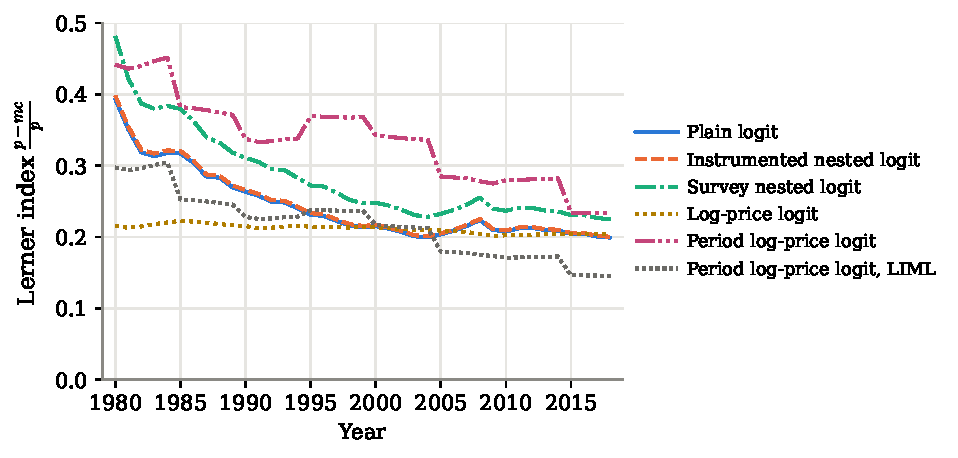
\includegraphics[width=0.95\linewidth]{figures/appC/autos_lerner.pdf}
\caption{Sales-weighted mean Lerner index of new vehicles by year under the six demand models of \cref{tab:C-autos}.
Computed with \texttt{figures/appC/src/autos\_markups.py} from the product data of the replication package of
\citet{GriecoMurryYurukoglu2024}.}
\label{fig:C-autos-lerner}
\end{figure}

\casehead{Part (c)}
Since $L_{jt} = \frac{m_{jt}}{p_{jt}}$, the log Lerner index splits exactly as
\begin{equation}\label{eq:C-lerner-decomp}
  \ln L_{jt} = \ln m_{jt} - \ln p_{jt} = \ln\big(\alpha_\ell m_{jt}\big) - \ln\alpha_\ell - \ln p_{jt} ,
\end{equation}
where $\alpha_\ell$ is the price coefficient that applies in year $t$. It is constant except in the period models of
part (d). We average with the weights $w_{jt}$ and difference between 1980 and 2018. The change in the mean log Lerner index
then splits into the change in the mean log dollar markup and the change in the mean log price. The dollar-markup term
splits again into a scaled markup $\alpha_\ell m_{jt}$ and the coefficient. For the logit with linear price the scaled
markup is $\frac{1}{1 - S_{ft}}$, a function of market structure alone.

\begin{table}[htbp]
\centering
\caption{Decomposition of the change in the mean log Lerner index, 1980 to 2018}
\label{tab:C-autos-decomp}
\footnotesize
\setlength{\tabcolsep}{4pt}
\begin{tabular}{@{}lcccccc@{}}
\toprule
 & Change in & \multicolumn{3}{c}{Dollar markup} & Price & Price share \\
\cmidrule(lr){3-5}
Model & $\overline{\ln L}$ & $\Delta\overline{\ln m}$ & $\Delta\overline{\ln(\alpha_\ell m)}$ & $-\Delta\ln\alpha_\ell$ &
$-\Delta\overline{\ln p}$ & of the fall (\%) \\
\midrule
Plain logit & $-0.694$ & $-0.050$ & $-0.050$ & 0 & $-0.644$ & 93 \\
Instrumented nested logit & $-0.700$ & $-0.056$ & $-0.056$ & 0 & $-0.644$ & 92 \\
Survey nested logit & $-0.765$ & $-0.122$ & $-0.122$ & 0 & $-0.644$ & 84 \\
Log-price logit & $-0.053$ & 0.591 & 0.591 & 0 & $-0.644$ & \\
Period log-price logit & $-0.636$ & 0.008 & 0.591 & $-0.583$ & $-0.644$ & 101 \\
Period log-price logit, LIML & $-0.710$ & $-0.067$ & 0.591 & $-0.658$ & $-0.644$ & 91 \\
\bottomrule
\end{tabular}

\vspace{3pt}
\begin{minipage}{0.97\textwidth}
\footnotesize Notes: Bars denote sales-weighted means within a year, and $\Delta$ the change from 1980 to 2018. The
first column equals the sum of the second and the fifth, and the second equals the sum of the third and the fourth. The
last column is $\frac{\Delta\overline{\ln p}}{-\Delta\overline{\ln L}}$ in percent, omitted where the index barely falls.
Computed with \texttt{figures/appC/src/autos\_markups.py}.
\end{minipage}
\end{table}

\Cref{tab:C-autos-decomp} shows that the decline in every model with a falling index is a fall relative to price. The
sales-weighted mean log price rose by 0.644. Under the plain logit the mean log Lerner index fell by 0.694, so rising
prices account for 93 percent of the fall. The dollar markup fell only 0.050 log points, because firm shares fell and
$\frac{1}{1 - S_{ft}}$ fell with them. The survey nested logit puts more weight on market structure, for a reason we
return to in part (d), but rising prices still account for 84 percent.

\casehead{Part (d)}
The \emph{log-price logit} replaces $\alpha p_{jt}$ by $\alpha\ln p_{jt}$. With the same instrument and controls,
$\hat\alpha = 5.109$ (1.687), and the first-stage $F$ statistic for $\ln p_{jt}$ is 25.1. By
\cref{prop:C-logit-lerner}(ii) the Lerner index stays near $\frac{1}{\hat\alpha} = 0.196$, and indeed it moves only from
0.216 to 0.204. The dollar markup now rises 81 percent, in step with prices. The decomposition shows the mechanism.
By \eqref{eq:C-logprice-markup} the scaled markup $\alpha m_{jt}$ is nearly proportional to price, so its mean log
rises by 0.591 and cancels most of the price term.

Neither functional form is innocuous, and the data can discriminate between them if the price coefficient may change
over time. The \emph{period log-price logit} gives each five-year period $\ell$ its own coefficient $\alpha_\ell$ on
$\ln p_{jt}$. The dollar price sensitivity, the utility lost per dollar, is then $\frac{\alpha_\ell}{p_{jt}}$. If
$\alpha_\ell$ rises in proportion to prices, dollar sensitivity is constant, as in the linear model. If $\alpha_\ell$ is
constant, we are back in the log-price model. Eight coefficients need eight excluded instruments at least. We interact
the exchange rate with period indicators and add assembly-country indicators interacted with period indicators, for
104 excluded instruments, with type-specific linear trends. The added instruments are valid if, within a make,
changes in unobserved quality across periods are unrelated to the assembly country. \citet[fn.~10]{GriecoMurryYurukoglu2024}
strengthen their first stage in the same way when they let the price coefficient vary over time.

\begin{table}[htbp]
\centering
\caption{Period-specific coefficients on log price}
\label{tab:C-autos-periods}
\footnotesize
\begin{tabular}{@{}lccccc@{}}
\toprule
 & \multicolumn{3}{c}{All 104 instruments} & \multicolumn{2}{c}{Exchange rate by period only} \\
\cmidrule(lr){2-4}\cmidrule(lr){5-6}
Period & 2SLS & LIML & OLS & 2SLS & Conditional $F$ \\
\midrule
1980--84 & 2.496 (0.506) & 3.703 & 1.521 & 1.679 (1.782) & 10.8 \\
1985--89 & 2.977 (0.441) & 4.502 & 1.233 & 7.251 (5.634) & 1.9 \\
1990--94 & 3.259 (0.558) & 4.818 & 1.413 & 5.343 (2.399) & 12.6 \\
1995--99 & 2.968 (0.607) & 4.609 & 1.405 & 4.996 (1.802) & 40.5 \\
2000--04 & 3.187 (0.548) & 5.037 & 1.526 & 3.459 (1.229) & 38.5 \\
2005--09 & 3.751 (0.539) & 5.951 & 1.944 & 4.994 (2.227) & 8.1 \\
2010--14 & 3.698 (0.662) & 6.040 & 2.333 & 6.329 (2.478) & 11.1 \\
2015--18 & 4.472 (0.653) & 7.148 & 2.461 & 5.223 (2.581) & 13.6 \\
\bottomrule
\end{tabular}

\vspace{3pt}
\begin{minipage}{0.97\textwidth}
\footnotesize Notes: Entries are $\hat\alpha_\ell$, the negative of the coefficient on $\ln p_{jt}$ in period $\ell$.
The first three columns use the exchange rate by period and assembly-country indicators by period as instruments. The
last two use the eight exchange-rate interactions only. All specifications include the controls of part (a) and
type-specific linear trends. Standard errors clustered by make. Conditional $F$ statistics follow
\citet{SandersonWindmeijer2016}. Computed with \texttt{figures/appC/src/autos\_markups.py}.
\end{minipage}
\end{table}

\Cref{tab:C-autos-periods} reports the coefficients. The 2SLS estimate of $\alpha_\ell$ rises from 2.50 in 1980--84 to
4.47 in 2015--18, an increase of 0.58 log points. Mean log price rose by 0.64, so dollar price sensitivity fell by only
0.06 log points. The dollar markup is then nearly flat (\$7,758 to \$7,851), and the Lerner index falls by 47 percent,
from 0.442 to 0.233. Once the coefficient may follow prices, the data choose a path close to the linear model. Two
caveats apply. With the exchange rate alone the period coefficients are imprecise, and the conditional $F$ statistic
falls to 1.9 in 1985--89, so the path rests on the assembly-country exclusions. With 104 instruments, 2SLS is also
biased toward OLS \citep{Bekker1994}. The OLS coefficients are much smaller, and the limited-information maximum
likelihood (LIML) estimates, which are less sensitive to many instruments, are 48 to 60 percent larger than 2SLS at the
two ends. LIML implies a rise of 0.66 log points in $\alpha_\ell$, lower Lerner indices at every date, and a fall of 51
percent.

The \emph{survey nested logit} replaces the weak instruments for $\sigma$ with information on substitution. A
second-choice survey reports, for buyers of each model, the model they considered most seriously. We treat it as the
model they would have bought had their first choice been unavailable. Its model
counterpart is the effect of removing the first choice from the choice set, a moment that \citet{BerryLevinsohnPakes2004}
introduced into demand estimation.

\begin{lemma}[Removing a model in the nested logit]\label{lem:C-nl-removal}
Suppose model $j$ in nest $g$ is removed and all mean utilities stay fixed. The remaining shares become
\begin{equation}\label{eq:C-nl-removal}
  s'_k = \frac{s_k(1 - s_{j\mid g})^{-\sigma}}{R_j} \ \text{ for } k \in g , \qquad
  s'_k = \frac{s_k}{R_j} \ \text{ otherwise} , \qquad
  R_j = 1 - s_g\big[1 - (1 - s_{j\mid g})^{1 - \sigma}\big] .
\end{equation}
\end{lemma}

\begin{proof}
Removing $j$ multiplies the inclusive sum of nest $g$ by $1 - s_{j\mid g}$, since
$s_{j\mid g} = \frac{e^{\frac{\delta_j}{1 - \sigma}}}{D_g}$, and leaves the other inclusive sums unchanged. The common
denominator $1 + \sum_hD_h^{1 - \sigma}$ is therefore multiplied by
$1 - s_g + s_g(1 - s_{j\mid g})^{1 - \sigma} = R_j$. A model $k \in g$ also has $D_g^{-\sigma}$ in its numerator, which is
multiplied by $(1 - s_{j\mid g})^{-\sigma}$. Substituting in \eqref{eq:C-nl-shares} gives \eqref{eq:C-nl-removal}.
\end{proof}

The survey records only second choices among new vehicles. The model probability that a buyer of $j$ names a second
choice of the same type is therefore
\begin{equation}\label{eq:C-sc-prob}
  \varphi_j(\sigma) = \frac{\sum_{k \in g, k \ne j}(s'_k - s_k)}{\sum_{k \ne j}(s'_k - s_k)} ,
\end{equation}
with both sums over inside models. At $\sigma = 0$ every remaining model gains in proportion to its share, so
$\varphi_j(0) = \frac{s_g - s_j}{1 - s_0 - s_j}$, the IIA answer. Larger $\sigma$ tilts the gains toward the nest. We choose
$\sigma$ so that the average of $\varphi_j(\sigma)$ over surveyed buyers, weighted by the number of respondents whose first
choice is $j$, equals the observed fraction of same-type second choices. That fraction is 84.6 percent. The plain logit
implies 38.2 percent and the instrumented nested logit 46.0 percent. Matching gives $\hat\sigma = 0.524$, with a
bootstrap standard error of 0.002 over the package's 500 resamples of the survey counts. Fitting each survey year
separately gives 0.478 for 1991, 0.567 for 1999, 0.519 for 2005 and 0.532 for 2015. The spread across years is much
larger than the bootstrap standard error, so that standard error understates the uncertainty about a common $\sigma$.

With $\sigma$ fixed at $\hat\sigma$, we move $\hat\sigma\ln s_{j\mid g,t}$ to the left side of \eqref{eq:C-nl-reg} and
estimate $\alpha$ by 2SLS with the exchange rate. Because 2SLS is linear in the dependent variable, the estimate is
$\hat\alpha(\sigma) = 1.696 - 1.795\,\sigma$, where 1.795 is minus the 2SLS coefficient on price in a regression of
$\ln s_{j\mid g,t}$. At $\hat\sigma = 0.524$ this gives $\hat\alpha = 0.755$. Its two-step standard error, which adds
$1.795^2$ times the variance of $\hat\sigma$, is 0.302. The model implies higher Lerner indices, 0.481 in 1980 and
0.225 in 2018, and a fall in the dollar markup of 12.3 percent. Market structure explains the larger fall. Nested logit markups depend on the firm's share within each type. The sales-weighted mean
within-type share of a model's firm fell from 0.280 to 0.137 as the number of models per type grew.

\casehead{Part (e)}
Four lessons emerge. First, simple models on the package data reproduce the broad decline. The plain logit and the
nested logits all put the 2018 index at about half its 1980 value. The full model of \citet{GriecoMurryYurukoglu2024}
gives a sales-weighted mean Lerner index of 0.42 in 1980 and 0.22 in 2018 (Section~5.4 and Table~VII), a ratio of
0.52. Our plain logit gives 0.393 and 0.199, a ratio of 0.506. We describe their model after the four lessons.

Second, the decline is a fall in markups relative to price. In every model except the log-price logit, the mean dollar
markup changes by between $-12.3$ and $+1.2$ percent, while the mean real price nearly doubles. Under linear price this
stability is built in, since by \cref{prop:C-logit-lerner} the dollar markup depends only on $\alpha$ and on shares. A
falling Lerner index with stable dollar markups is what rising quality and marginal cost produce. It does not mean that
firms earn less per vehicle.

Third, the functional form of price decides the trend once the price coefficient is held fixed. Linear price builds in
a Lerner index proportional to $\frac{1}{p}$, and log price builds in a flat one. \citet{GriecoMurryYurukoglu2024}
report a much smaller decline in their own log-price specification, from 0.32 to 0.27 (Section~5.4). With log price
and a separate coefficient for each five-year period, their path looks very similar to their baseline (Figure~VIb).
When the coefficient on log price may change over time, our estimates also move it almost in proportion to prices,
which supports the linear form. That conclusion rests on 104 instruments and on exclusions by assembly country. A cost shifter
that varies more across periods, such as wages in the assembly countries, would test it directly.

Fourth, the substitution parameters matter for levels more than for trends. The survey nested logit raises the Lerner
index by about 0.09 in 1980 and 0.03 in 2018 relative to the plain logit. Aggregate data alone cannot pin down $\sigma$
(\cref{tab:C-autos-nl}), and the second-choice survey can. This is the same lesson as in \cref{sec:C-rc-est}, where the
logit understated diversion among inside goods.

The full model of \citet{GriecoMurryYurukoglu2024} differs from ours in its demand system, its data and its estimator.
Their demand is a random coefficients logit in the tradition of \citet{BerryLevinsohnPakes1995}. In our notation,
household $i$ in year $t$ obtains
\begin{equation}\label{eq:C-gmy-utility}
  u_{ijt} = x_{jt}\beta_{it} - \alpha_{it}p_{jt} + \xi_{jt} + \epsilon_{ijt} , \qquad u_{i0t} = \gamma_t + \epsilon_{i0t} ,
\end{equation}
from model $j$ and from the outside good (their eq.~1). The value $\gamma_t$ of not buying a new vehicle changes from
year to year. Let $D_{it}$ be the vector of household demographics, drawn from the CPS. It has nothing to do with the
inclusive sums $D_{gt}$ of part (a). The coefficients are
\begin{equation}\label{eq:C-gmy-coef}
  \alpha_{it} = \alpha + \pi^\top D_{it} , \qquad \beta_{ikt} = \beta_k + \Pi_kD_{it} + \Sigma_{kk}\nu_{ik} ,
\end{equation}
where $\Pi_k$ is the $k$-th row of $\Pi$ and the $\nu_{ik}$ are independent standard normal draws (eqs.~3--4). The
parameters are fixed over time, but the distribution of tastes moves as demographics change. In our sign convention the
mean price coefficient is $\alpha = 3.112$ (1.124) per \$10,000 (Table~IV). Price sensitivity varies with income, its
square and age. Family size shifts the tastes for vans and for footprint, and rural households value trucks more. Eleven
characteristics carry random coefficients. The two largest are on vehicle types, 6.309 for trucks and 5.538 for vans.
The SUV coefficient of 3.617 is close to the largest remaining one, 3.798 for electric vehicles. The type coefficients
play the role of our nests, since a household with a strong taste for trucks substitutes mainly among trucks.

The year effects mix two objects. GMY write $\xi_{jt} = \tau_t + \tilde\xi_{jt}$, where $\tau_t$ is the mean
unobserved quality of the models of year $t$ relative to the base year. Shares identify only the difference
$\tau_t - \gamma_t$. Following \citet{PakesBerryLevinsohn1993}, GMY assume that unobserved quality does not change on
average for models that continue from $t - 1$ to $t$ without a redesign. With $\mathcal{C}_t$ the set of such models,
\begin{equation}\label{eq:C-gmy-continuing}
  \E\big[\xi_{jt} - \xi_{j,t-1}\big] = \E\big[(\tau_t - \tau_{t-1}) + (\tilde\xi_{jt} - \tilde\xi_{j,t-1})\big] = 0
  \qquad \text{for } j \in \mathcal{C}_t ,
\end{equation}
with the normalization $\tau_0 = 0$ (eq.~2). The condition separates better vehicles from a more attractive outside
option. Mean unobserved quality rises roughly linearly, by about \$25,000 over the period (Section~5.2).

Estimation has three steps (Section~5). The first step chooses the demographic interactions, the random coefficients
and the mean utilities by GMM. It matches two kinds of micro moments. The CEX (1980--2005, about 1,014 buyers a year)
and MRI (1992--2018, about 2,005 buyers a year) give moments such as the mean price paid in each income quintile
(Sections~2.3 and~5). The MaritzCX survey gives the correlations between the attributes of first and second choices in the
four survey years. The second step regresses the mean utilities on characteristics, price, make dummies and year
dummies by 2SLS, with the lagged real exchange rate as the excluded instrument. This is the moment condition of our part
(a). The third step splits the year effects into $\tau_t$ and $\gamma_t$ with \eqref{eq:C-gmy-continuing}. Standard
errors come from 500 bootstrap samples of the micro data, with a nested parametric bootstrap, clustered by make, in the
second step.

Each source of variation has a clear role. The real exchange rate is the price level of the assembly country relative
to the United States, taken from the Penn World Table and lagged one year (Section~2.2). It moves with local wages and
with the nominal exchange rate, and both shift the dollar cost of the vehicles made there. It identifies the price
coefficient. The second choices identify the random coefficients. The correlation between the truck indicators of first
and second choices is 0.843 in the data and 0.798 in the full model (Table~VI). A model with the demographic
interactions alone gives $-0.013$, and the logit gives $-0.024$. Observed heterogeneity alone cannot produce the
substitution within types that the survey records. Our survey nested logit in part (d) rests on the same evidence.

The full model gives a share-weighted mean own-price elasticity of $-5.06$ over the sample (Section~5.1). The market
elasticity is $-1.07$ in 1985 and $-1.29$ in 2015 (Table~V). The median Lerner index falls from 0.325 to 0.185
(Figure~VIa). The decline survives a linear trend in the price coefficient, a separate coefficient for each five-year
period and separate estimation on three subperiods (Figure~VIb).

GMY explain the decline much as part (c) does. Single-product markups follow nearly the same path as multi-product ones
(Figure~VIIIa). The single-product rule $L_{jt} = -\frac{s_{jt}}{p_{jt}}\big(\frac{\partial s_{jt}}{\partial
p_{jt}}\big)^{-1}$ of their eq.~(7) therefore guides the reading. From 1980 to 1999, mean shares and mean own-price
derivatives stay flat while mean prices rise, so the index falls. Counterfactuals then isolate the primitive forces
(Section~5.4.1). Removing the growth of foreign brands from the ownership structure, or holding the number of products
at its 1980 level, does not remove the decline. Mapping each year's characteristics onto their 1980 distribution keeps
marginal costs flat and substantially reduces the fall (Figure~IX). In their reading, better vehicles raised marginal
costs, which were passed through to prices less than fully.

GMY maintain Nash-Bertrand pricing and ask how much collusion would be needed to undo the decline (Section~5.5).
Simulated cartels in 2018 answer the question in Table~VII. A cartel of GM, Ford and Toyota raises the mean Lerner index
only to 0.26. Only a cartel of the six largest parent companies, at 0.46, exceeds the 1980 value of 0.42. The
Herfindahl index meanwhile fell from 2,661 to 1,132 points. Beyond markups, the consumers' share of efficient surplus
rose from 0.62 to 0.82, and consumer surplus per household rose by about \$8,000 (Section~1). GMY define efficient
surplus as consumer surplus plus producer surplus plus deadweight loss, the surplus at prices equal to marginal costs.
Our simple models agree with the full model on the main mechanism. Prices rose against stable dollar markups. GMY
report no dollar markups. By their eq.~(7), however, flat mean shares and own-price derivatives imply flat
single-product dollar markups from 1980 to 1999 (Section~5.4.1 and Figure~VIII). What the full model adds is the separation of
quality from the outside option and a measure of welfare.

The exercise has clear limits. Prices are list prices, so changes in discounts and rebates over time pass into the
estimated markups. The market size of one vehicle per 2.5 households is a convention, and the outside share moves with
it. Demand is static, with no used-car market or replacement timing, and the nests are chosen a priori. The exchange
rate may violate the exclusion if currency movements coincide with changes in a make's unobserved quality. The
comparison with production-function estimates is also less direct than it looks. The demand-side Lerner index measures
price over marginal cost for new vehicles, while production-function markups use firm-level revenue and variable
input costs (\cref{sec:01-rising-markups}). \citet[Section~5.6]{GriecoMurryYurukoglu2024} make this comparison for the
auto industry. Both the level and the trend of their ratio of price to marginal cost differ from the production-function
series, although both are fairly flat after 1995. What the exercise contributes is a diagnosis. It shows which parts of a
measured trend in markups come from the data, which from the functional form, and which from the estimated
substitution patterns.

\subsection{Computational notes}

The script \texttt{autos\_markups.py} reads the package files \texttt{data\_blp.csv}, \texttt{secondChoiceOut.mat}
and \texttt{secondChoice\_bootstrap.mat}, and it runs in about three minutes.
\begin{enumerate}
  \item Build shares with $M_t$ equal to households divided by 2.5, prices in \$10,000, nests from the type indicators,
  and within-type shares and counts by year and type.
  \item Code 2SLS, the clustered sandwich, first-stage and conditional $F$ statistics and LIML with numpy. Run the
  logit, the nested logit grid and the log-price models.
  \item Fit $\sigma$ to the second-choice counts with a bracketing root finder on $[0, 0.995]$, using
  \eqref{eq:C-nl-removal} and \eqref{eq:C-sc-prob}, and repeat for each bootstrap sample of counts.
  \item For each model and year, form $\Delta_t$ from \eqref{eq:C-nl-deriv} or its log-price analogue and solve
  \eqref{eq:C-autos-markup} with the parent-company ownership matrix.
  \item Check the share inversion, the removal formula against brute-force removal, the derivatives against finite
  differences and the logit markups against \cref{prop:C-logit-lerner}.
\end{enumerate}


\section{Bibliographic notes}\label{sec:C-notes}

The cross-industry regressions of margins on concentration that \cref{sec:C-cournot} examines go back to
\citet{Bain1951}, and \citet{Schmalensee1989} reviews the evidence they produced. \citet{CowlingWaterson1976} derived
the Cournot relation between the Herfindahl index and the share-weighted Lerner index. \citet{Demsetz1973} stated
the efficiency critique that \cref{prop:C-demsetz} formalizes. \citet[Section~5.5]{Tirole1988} develops both results as
exercises, together with the welfare bound of \citet{DansbyWillig1979}. The merger paradox of Cournot competition is
due to \citet{SalantSwitzerReynolds1983}. \citet{FarrellShapiro1990} derive the general synergy condition for a Cournot
merger to lower price and a sufficient condition for it to raise welfare. \citet[Section~3.3]{AskerNocke2021} survey
the theory of unilateral merger effects built on that analysis, including mergers among multi-product logit firms and
mergers under free entry. \citet{MankiwWhinston1986} established the excess-entry result. Grim-trigger strategies
come from \citet{Friedman1971}, and \citet{Abreu1986} characterized the optimal punishments that sustain collusion at
lower discount factors. \citet[Section~6.3.2.1]{Tirole1988} uses the Bertrand supergame to link concentration with
tacit collusion.

\citet{Sumner1981} introduced the tax pass-through test of \cref{sec:C-passthrough}. The link between pass-through
and the curvature of demand goes back to \citet{BulowPfleiderer1983}, and \citet{WeylFabinger2013} develop it into a
general framework for incidence under imperfect competition. \citet{Barzel1976} raised the quality response to unit
taxes. \citet{Bresnahan1982} and \citet{Lau1982} showed that parallel shifts of demand cannot separate conduct
from marginal cost. Demand rotations, which change the slope of demand at a given price, can. \citet{Bresnahan1989}
restates this argument in his survey of conduct estimation. \citet{Corts1999} shows that an estimated conduct
parameter can badly mismeasure market power when firms collude tacitly in a repeated game.
\citet{BertrandDufloMullainathan2004} documented how serial correlation overstates the precision of
difference-in-differences regressions, the same problem that clustering addresses in \cref{sec:C-passthrough}.

For logit pricing, \citet{CaplinNalebuff1991} proved existence of price equilibrium under $\rho$-concavity conditions
on the distribution of tastes, which are weaker than log-concavity. They proved uniqueness in cases that include
single-product logit firms, and they credit \citet{AndersonDePalma1988} with the first uniqueness result for the logit
duopoly.
\citet{KonovalovSandor2010} extended uniqueness to multi-product logit firms, and \citet{NockeSchutz2018} developed
the aggregative approach used in \cref{prop:C-unique}. \citet{MorrowSkerlos2011} proposed the fixed-point
formulation that \cref{sec:C-simulate} uses to compute random coefficients equilibria. The upward pricing pressure of
\cref{sec:C-logit-bertrand} is due to \citet{FarrellShapiro2010}, and \citet{Werden1996} derived the compensating
marginal cost reductions of the further problems below.

The estimation problems rest on \citet{Berry1994}, who introduced the share inversion and applied it to the logit,
the nested logit and the vertical model. The vertical model of \cref{sec:C-vertical} follows \citet{Bresnahan1987}
and his study of the 1955 automobile market, which finds collusive pricing in 1954 and 1956 and competitive pricing in
1955. \citet{BerryLevinsohnPakes1995} developed the random coefficients model, its
contraction and its instruments, and \citet{Nevo2000a} gives a practical guide to its estimation.
\citet{ConlonGortmaker2020} collect current best practice for computation and instruments, including the
differentiation instruments of \citet{GandhiHoude2019}. \citet{DubeFoxSu2012} show how loose inner-loop tolerances
distort the estimates. \citet{BerryLevinsohnPakes2004} brought second-choice data into demand estimation, and
\citet{SandersonWindmeijer2016} give the weak-instrument diagnostics for several endogenous regressors that
\cref{sec:C-autos} uses. The question of \cref{sec:C-autos} comes from \citet{GriecoMurryYurukoglu2024}. They estimate
a random coefficients logit with demographic micro moments and second-choice data. They separate unobserved quality
from the value of the outside good with the continuing-products restriction of \citet{PakesBerryLevinsohn1993}. They
find that the mean Lerner index of new vehicles roughly halved from 1980 to 2018. The production-function evidence on rising markups that motivates the question is in \citet{DeLoeckerEeckhoutUnger2020}.

\section{Further problems}\label{sec:C-further}

The following problems extend the worked problems. Solutions are not provided.

\begin{enumerate}
\item \emph{Cournot with constant-elasticity demand.} Let inverse demand be $P(Q) = AQ^{-\frac{1}{\varepsilon}}$ with
  $\varepsilon > 1$, and let firm $i$ have constant marginal cost $c_i$ and fixed cost $F$. Show that every active firm
  satisfies $L_i = \frac{s_i}{\varepsilon}$. With symmetric costs, find the free-entry number of firms, treating it as
  continuous, and the resulting $L$ and $\HHI$. Compare the relation between concentration and margins across
  industries that differ in $A$ or in $F$ with the linear case of \cref{sec:C-cournot}, part (d).

\item \emph{One-period punishments.} In the repeated linear Cournot game of \cref{sec:C-cournot}, part (c), let inverse
  demand be $P(Q) = \max\{a - bQ, 0\}$. After a deviation every firm produces $q^p$ for one period and then returns to
  $\frac{Q^m}{N}$. Write the incentive constraints of the collusive phase and of the punishment phase. For $N = 2$ and
  the parameters of \cref{sec:C-cournot}, part (g), find numerically the lowest discount factor at which some $q^p$
  satisfies both constraints, and compare it with $\delta^*(2) = \frac{9}{17}$ \citep{Abreu1986}.

\item \emph{An ad valorem tax in the logit market.} In the 25-product market of \cref{sec:C-logit-bertrand}, firms
  receive $(1 - \tau)p_j$ per unit sold. Derive the single-product and multi-product first-order conditions, compute the
  equilibria at $\tau = 0.1$, and report the elasticity of each price with respect to $\frac{1}{1 - \tau}$. Compare the
  results with \cref{prop:C-adval} and explain the role of the curvature of logit demand.

\item \emph{Compensating marginal cost reductions with random coefficients.} \Cref{ex:04-merger-sim} computes the
  reductions in marginal cost that leave every price unchanged after the logit merger of \cref{sec:C-logit-bertrand},
  part (g) \citep{Werden1996}. Consider instead the merger of firms B and C in market 0 of \cref{sec:C-rc-est},
  part (f). Show that, for any demand model, the compensating marginal costs are
  $mc' = p + (\Omega' \odot \Delta^\top)^{-1}s$, with $\Omega'$ the post-merger ownership matrix and $\Delta$ and $s$
  evaluated at pre-merger prices. Explain why the costs of non-merging products are unchanged. Compute the reductions
  under the logit, the estimated random coefficients model and the true model, and compare them with the upward
  pricing pressure in \cref{tab:C-merger-m0}.

\item \emph{The vertical model with uniform tastes.} Let the price sensitivity $\nu_i$ be uniform on
  $[0, \bar\nu]$. Redo parts (a) to (c) of \cref{sec:C-vertical}. Which parameters are identified, and do the implied
  markups depend on $\bar\nu$? Compare the implied own elasticities in market 0 with \cref{tab:C-velast}. Then let the
  taste for quality $\frac{1}{\nu_i}$ be uniform instead, the specification of \citet{Bresnahan1987}, and derive the
  inversion again.

\item \emph{How many simulation draws?} Let $s^{n_s}_{jt} = \frac{1}{n_s}\sum_{i=1}^{n_s}s_{ijt}$ with independent
  draws $\nu_i$. Show that $\Var(s^{n_s}_{jt}) = \frac{1}{n_s}\Var_\nu(s_{ijt})$. With the firms' draws of
  \cref{sec:C-simulate}, estimate the number of draws that gives a relative standard error of one percent for every
  product in market 0. Compare this simulation error with the sampling error of the realized shares.

\item \emph{Differentiation instruments.} Replace the six competition instruments of \cref{sec:C-logit-est} by two
  counts \citep{GandhiHoude2019}. The first counts rival products whose sugar content lies within one standard
  deviation of the product's own. The second counts rival products with the same organic status. Re-estimate the logit by 2SLS and the random
  coefficients model of \cref{sec:C-rc-est} with $\Sigma$ known. Report the first-stage statistics and explain why the
  new instruments are or are not stronger.

\item \emph{Nested logit pricing.} With nested logit demand and multi-product firms, derive the first-order
  conditions for prices. Show that markups are common within each pair of a firm and a nest, and give the formula
  for the common markup in terms of the firm's within-nest and total shares. When does the formula reduce to the
  single-product markup of \cref{prop:C-nl-deriv}?
\end{enumerate}
